\documentclass{createspace}
\newcommand{\N}{\mathbb N}
\newcommand{\Z}{\mathbb Z}
\newcommand{\Q}{\mathbb Q}
\newcommand{\R}{\mathbb R}
\newcommand{\C}{\mathbb C}

\newcommand{\shrap}{\mathbin{\#}}
\DeclareMathOperator*{\bigshrap}{\#}

\newcommand{\bracket}[1]{\left\langle{#1}\right\rangle}

\newcommand{\alexander}{\Delta}
\newcommand{\conway}{\nabla}
\newcommand{\jones}{V}
% span?

\newcommand{\braid}{\operatorname{b}}
\newcommand{\bridge}{\operatorname{br}}
\newcommand{\crossing}{\operatorname{cr}}
\newcommand{\genus}{\operatorname{g}}
\newcommand{\linking}{\operatorname{lk}}
\newcommand{\ropelength}{\operatorname{len}}
\newcommand{\sign}{\operatorname{sgn}}
\newcommand{\stick}{\operatorname{s}}
\newcommand{\unknotting}{\operatorname{u}}
\newcommand{\volume}{\operatorname{vol}}
\newcommand{\writhe}{\operatorname{wr}}

\newcommand{\inversedcurvearrowright}{\rotatebox[origin=c]{180}{$\curvearrowleft$}}
\newcommand{\inversedcurvearrowleft}{\rotatebox[origin=c]{180}{$\curvearrowright$}}

\usepackage{enumitem}
\usepackage{booktabs}
\usepackage{longtable}
\usepackage[table]{xcolor}
\usepackage[colorinlistoftodos,prependcaption]{todonotes}
\usepackage{tikz}
\usetikzlibrary{arrows.meta}
\usetikzlibrary{decorations.markings}
\usetikzlibrary{decorations.pathreplacing}
\usetikzlibrary{knots}
\colorlet{darkblue}{blue!80!black}
\newcommand{\MalyNieWezel} {\begin{tikzpicture}[baseline=-0.65ex, scale=0.02]
	\begin{knot}[clip width=5, end tolerance=1pt]
		\strand[semithick] (0,0) circle (5);
	\end{knot}
\end{tikzpicture}}

\newcommand{\NieWezel} {\begin{tikzpicture}[baseline=-0.65ex, scale=0.04]
	\begin{knot}[clip width=5, end tolerance=1pt]
		\strand[semithick] (0,0) circle (5);
	\end{knot}
\end{tikzpicture}}

\tikzset{
	->-/.style={decoration={markings, mark=at position .5 with {\arrow{>}}},postaction={decorate}},
	-<-/.style={decoration={markings, mark=at position .5 with {\arrow{<}}},postaction={decorate}},
	LUK/.style ={
		draw=black,
		line join=miter,
		line cap=butt,
		miter limit=4.00,
		line width=0.2 mm
	},
	CIENKILUK/.style ={
		draw=black,
		line join=miter,
		line cap=butt,
		miter limit=4.00,
		line width=0.1 mm
	},
	TEKSTOWY/.style ={
		draw=black,
		line join=round,
		line cap=butt,
		miter limit=20.00,
		line width=0.2 mm
	},
	OBSZAR/.style={
		draw=none,
		fill=white!#1!red
	},
	OBSZAR/.default = 80,
}

\author{Leon Suwalski}
\title{Krótkie wprowadzenie do teorii węzłów (wersja robocza)}
\date{2018}

\begin{document}
\maketitle
\tableofcontents
\chapter{Preludium}
\label{cha:preludium}
Teoria węzłów to gałąź topologii,
która powstała z~inspiracji węzłami,
jakie pojawiają się w~codziennym życiu: przy wiązaniu butów albo cumowaniu statków.
Zajmuje się ona badaniem przede wszystkim węzłów,
czyli pewnych włożeń okręgu $S^1$ w~trójwymiarową przestrzeń euklidesową $\R^3$ lub sferę $S^3$,
ale także splotów (zaplątanych w~sobie węzłów), warkoczy, supłów oraz podobnych obiektów.
Matematyczne węzły różnią się tym od zwykłych, że ich końce są ze sobą połączone.

Oto kilka przykładów.
Węzeł (a) nazywamy niewęzłem (jest to kalka angielskiego \emph{unknot}).
Następne w~kolejce widoczne są trójlistnik (b,~\emph{trefoil}), ósemka (c,~\emph{figure-eight}), pięciolistnik (d,~\emph{cinquefoil}) oraz słynna para Perko (e,~f~wg oryginalnej numeracji Rolfsena).

\begin{figure}[H]
    \centering
    \begin{minipage}[b]{.14\linewidth}
        \centering
        $\begin{tikzpicture}[baseline=-0.65ex, scale=0.5] \begin{knot}[clip width=5, end tolerance=1pt] \strand[semithick] (0,0) circle (\linewidth); \end{knot}
\end{tikzpicture}$
        \subcaption{}
    \end{minipage}
    \begin{minipage}[b]{.14\linewidth}
        \centering
        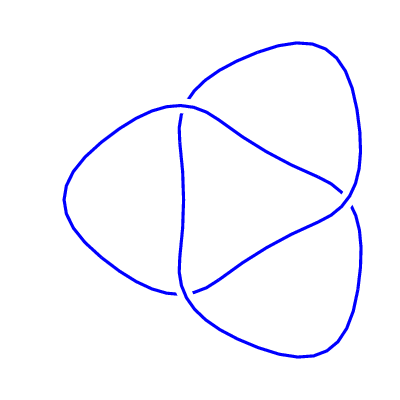
\includegraphics[width=\linewidth]{../data/3_1.png}
        \subcaption{$3_1$}
    \end{minipage}
    \begin{minipage}[b]{.14\linewidth}
        \centering
        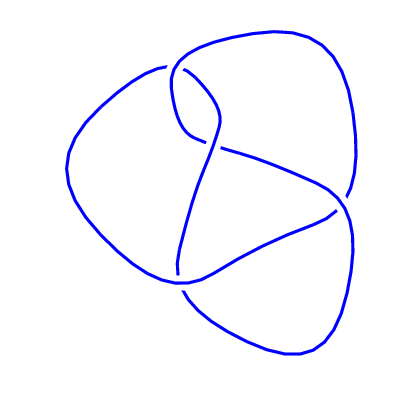
\includegraphics[width=\linewidth]{../data/4_1.png}
        \subcaption{$4_1$}
    \end{minipage}
    \begin{minipage}[b]{.14\linewidth}
        \centering
        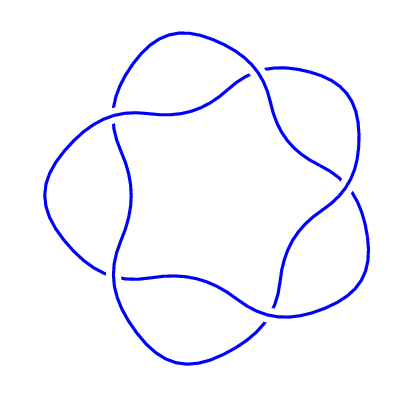
\includegraphics[width=\linewidth]{../data/5_1.png}
        \subcaption{$5_1$}
    \end{minipage}
    \begin{minipage}[b]{.14\linewidth}
        \centering
        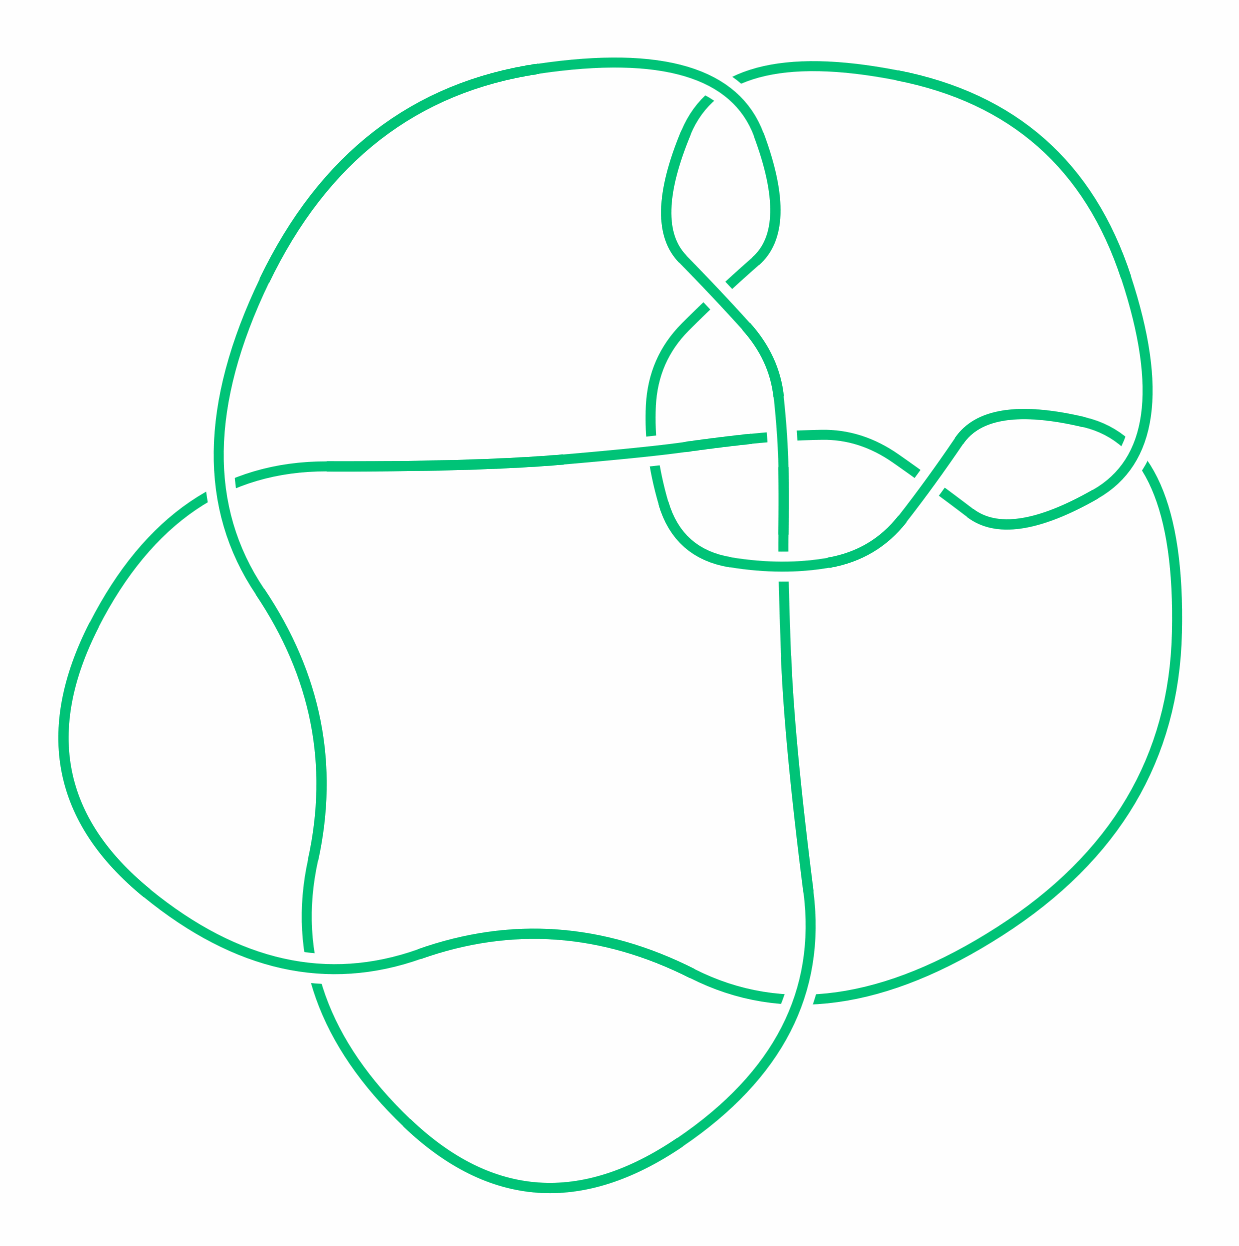
\includegraphics[width=\linewidth]{../data/perko1.png}
        \subcaption{$10_{161}$}
    \end{minipage}
    \begin{minipage}[b]{.14\linewidth}
        \centering
        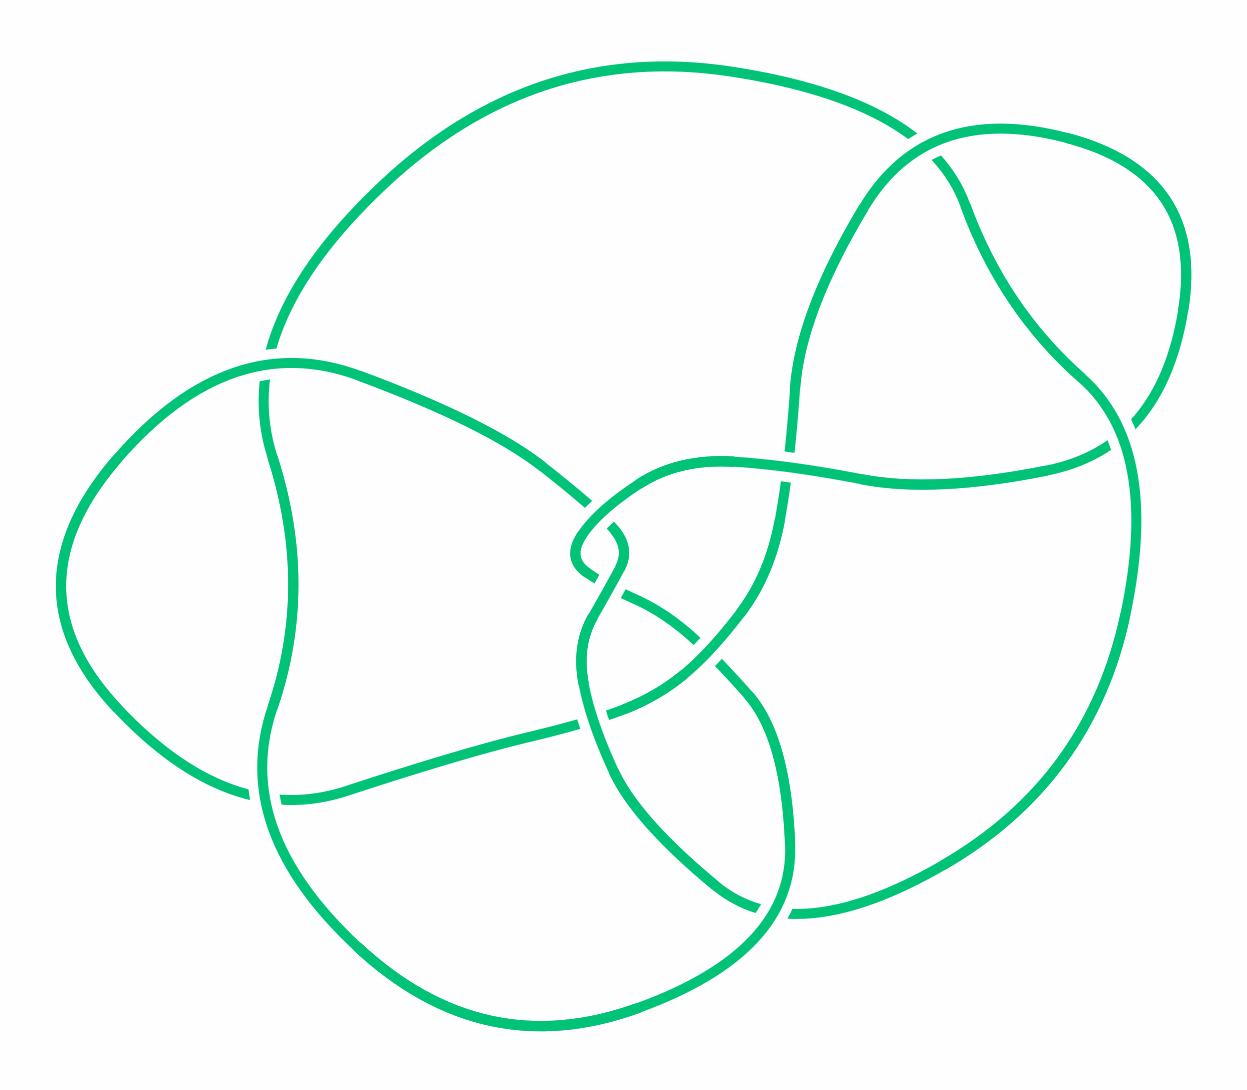
\includegraphics[width=\linewidth]{../data/perko2.png}
        \subcaption{$10_{162}$}
    \end{minipage}
\end{figure}

Początkowo celem teorii węzłów była klasyfikacja wszystkich węzłów.
Od XIX wieku, kiedy teoria węzłów wyodrębniła się jako osobny dział matematyki,
zdążyliśmy skatalogować ponad sześć miliardów tych obiektów.
Pozornie tak samo wyglądające węzły mogą się od siebie różnić.
Do wykrywania tych subtelnych różnic używa się przede wszystkim niezmienników topologicznych takich jak grupy, wielomiany bądź liczby.
Poznamy je w~dalszych rozdziałach.

Matematycy uogólnili pojęcie węzła:
można rozpatrywać je w~wyższych wymiarach albo zastąpić okrąg inną przestrzenią topologiczną.
Będziemy starać się unikać tych uogólnień.

\section{Węzły i~sploty}
Największą różnicą między węzłami matematycznymi oraz tymi z~prawdziwego jest życia jest to, że te pierwsze nie mają luźnych końców.
Można przyjąć nieidealną, naiwną definicję:

\begin{definition}[węzeł?]
    Ciągłe oraz różnowartościowe odwzorowanie $S^1 \to \R^3$ nazywamy węzłem.
\end{definition}

Zastanówmy się, jakim formalizmem opisać manipulowanie fizycznym sznurkiem.
Nie można użyć izotopii
(dwa węzły są izotopijne, jeśli istnieje ciągła funkcja $F \colon S^1 \times [0, 1] \to \R^3$ taka, że $F(-, 0)$ jest pierwszym, zaś $F(-,1)$ drugim węzłem).
Zauważmy, że każde splątanie ściąga się do punktu.
Dowolny węzeł jest równoważny z~trywialnym, zatem istnieje tylko jedna klasa abstrakcji.
Trzeba uwzględnić to, jak węzeł leży w~przestrzeni.
Właściwym narzędziem jest więc izotopia otaczająca.
Intuicyjnie: dwa węzły uznajemy za równoważne,
jeśli można przejść od jednego do drugiego przy użyciu deformacji całej przestrzeni $\R^3$.

\begin{definition}[izotopia otaczająca] \label{def_ambient_isotopy}
    Ciągłe odwzorowanie $F \colon \R^3 \times [0,1] \to \R^3$,
    które staje się homeomorfizmem po ustaleniu drugiego argumentu i~takie,
    że $F(-, 0)$ jest funkcją tożsamościową,
    zaś $F(-, 1)$ złożona z~pierwszym węzłem daje drugi węzeł,
    nazywamy izotopią otaczającą.
\end{definition}

\begin{definition}[węzeł]
    \label{def:knot}
    \index{węzeł}
    Gładkie włożenie $S^1 \to \R^3$ izotopijne otaczająco z~zamkniętą łamaną bez samoprzecięć nazywamy węzłem poskromionym.
\end{definition}

Wykluczamy w~ten sposób patologiczne z~kombinatorycznego punktu widzenia węzły dzikie.
Przez prawie całą książkę interesować nas będą jedynie węzły poskromione,
dlatego jeśli nie zaznaczono inaczej, przez węzeł rozumiemy węzeł poskromiony.

\begin{figure}
    \centering
    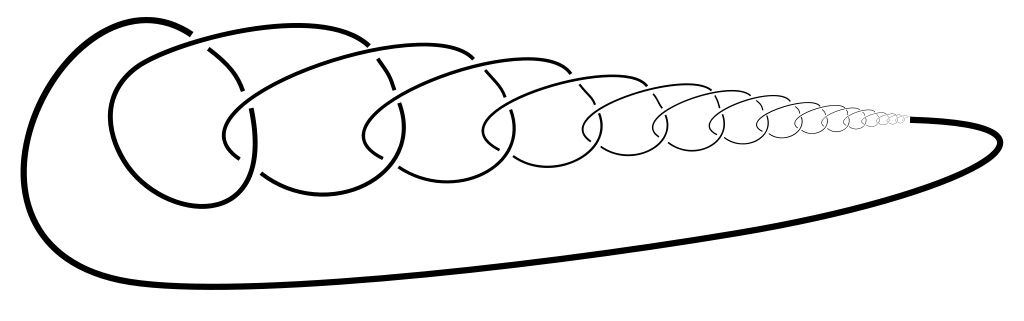
\includegraphics[width=0.5\linewidth]{wild_knot.png}
    \caption{Węzeł dziki}
\end{figure}

Dość często będziemy utożsamiać węzeł z~jego obrazem.

Jednocześnie homeomorfizmy $F(-,t)$ zastępujemy przez dyfeomorfizmy zachowujące orientację.
Chwila namysłu wystarcza do przekonania się, że definicja \ref{def_ambient_isotopy} obejmuje zwykłą izotopię,
a przy tym nie pozwala na rozwiązanie nietrywialnych węzłów przez ściągnięcie zaplątania do punktu.
Istnieje jeszcze jedna, konkurencyjna definicja węzłów równoważnych:

\begin{definition}
    \label{equivalent_knots_2}
    Dwa węzły są równoważne, gdy jeden z~nich jest obrazem drugiego przez zachowujący orientację homeomorfizm $\R^3 \to \R^3$.
\end{definition}

Stwierdzenie to przestaje być prawdziwe po zastąpieniu przestrzeni $\R^m$ przez $S^m$.

\begin{proof}
    Podany niżej dowód pochodzi z~książki ,,Topology from the differentiable viewpoint'' Johna Milnora.
    Musimy pokazać, że dyfeomorfizm $f \colon \R^m \to \R^m$ jest gładko izotopijny z~identycznością.
    Translacje są izotopiami, więc bez straty ogólności zakładamy, że $f(0) = 0$.
    Pochodna $f$ w~zerze jest dana wzorem $\mathrm{d}f_0(x) = \lim_{t \to 0} f(tx) /t$,
    naturalną definicją    izotopii $F \colon \R^m \times [0, 1] \to \R^m$ jest więc
    \[
        F(x, t) = \begin{cases}
            f(tx) / t & 0 < t \le 1 \\
            \mathrm{d}f_0(x) & t = 0
        \end{cases} .
    \]

    Funkcja $F$ jest gładka,
    gdyż na mocy lematu Hadamarda funkcja $f$ zapisuje się jako suma $x_1 g_1(x) + \ldots + x_mg_m(x)$,
    gdzie funkcje $g_i$ są gładkie, co jakoś kończy dowód.
\end{proof}

\begin{definition}[splot]
    \label{def_link}
    \index{splot}
    Sumę rozłączną skończenie wielu węzłów nazywamy splotem.
\end{definition}

Podobnie jak dla węzłów mówimy, że dwa sploty są równoważne, jeśli jeden jest obrazem drugiego przez zachowujący orientację homeomorfizm $\R^3 \to \R^3$.
Wtedy obydwa sploty mają tyle samo składowych.

\begin{example}
    \index{splot!Hopfa}
    Whitehead w~1934 odkrył kontrprzykład do nieudanego dowodu hipotezy Poincarego.
    Był nim splot o~dwóch składowych przedstawiony na poniższym rysunku.
    Splot Hopfa to najprostszy splot nietrywialny, którym w~1931 r. zajmował się Heinz Hopf,
    topolog niemiecki, w~ramach badań nad tzw. rozwłóknieniem (Hopf fibration).

    \begin{figure}[H]
        \begin{minipage}[b]{.48\linewidth}
            \centering
            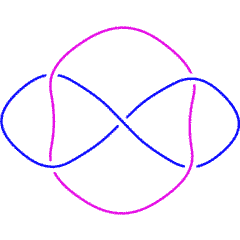
\includegraphics[width=0.5\linewidth]{../data/mixed/L5a1.png}
            \subcaption{splot Whiteheada}
        \end{minipage}
        \begin{minipage}[b]{.48\linewidth}
            \centering
            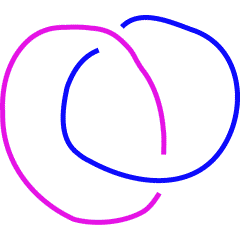
\includegraphics[width=0.5\linewidth]{../data/mixed/L2a1.png}
            \subcaption{splot Hopfa}
        \end{minipage}
    \end{figure}
\end{example}

\begin{definition}[rozszczepialność]
    \index{splot!rozszczepialny}
    Splot, który jest niespójną sumą niepustych splotów, nazywamy rozszczepialnym.
\end{definition}

Jeśli dwa węzły są równoważne, to ich dopełnienia są oczywiście homeomorficzne.
Pytanie o~prawdziwość implikacji odwrotnej jako pierwszy zadał najprawdopodobniej w~1908 roku Tietze (,,Über die topologischen Invarianten mehrdimensionaler Mannigfaltigkeiten'').
Od 1989 roku znamy odpowiedź na nie, jest pozytywna: każdy węzeł jest wyznaczony jednoznacznie przez swoje dopełnienie.
Wcześniej pokazano, że istnieją co najwyżej dwa węzły o~zadanym dopełnieniu.

\begin{theorem}[Gordon, Luecke, 1989] \label{thm_gordon_luecke}
    \index{twierdzenie!Gordona-Lueckego}
    Poskromione węzły o~homeomorficznych (z zachowaniem orientacji) dopełnieniach są wzajemnie izotopijne.
\end{theorem}

Twierdzenie to zamienia problem lokalny (czy dwa węzły w kuli $S^3$ są równoważne?) w~problem globalny (czy dwie przestrzenie topologiczne są homeomorficzne?).

\begin{proof}[Niedowód]
    Wynika to z~ogólniejszego stwierdzenia:
    nietrywialna chirurgia Dehna na węźle w~3-sferze nigdy nie daje 3-sfery.
    Pełny dowód zawiera praca \cite{gordon89}.
\end{proof}

Istnieje nieskończenie wiele (jakich?) kontrprzykładów do odpowiednika twierdzenia Gordona-Lueckego dla splotów,
których nie da się, patrząc na samo dopełnienie, odróżnić od splotu Whiteheada.

\section{Diagramy}
Chociaż w~świetle definicji \ref{def:knot} węzły są pewnymi regularnymi podzbiorami przestrzeni $\R^3$,
z kombinatorycznego punktu widzenia wygodniej jest rysować je na  płaszczyźnie.

\begin{definition} [diagram] \label{def_diagrams}
    \index{diagram}
    Cień to rzut węzła $K \subseteq \R^3$ na płaszczyznę.
    Diagram to cień bez katastrof
    (potrójnych przecięć, stycznych i~dziobów)
    razem z~informacją o~tym, jak przebiegają skrzyżowania.
\end{definition}

\begin{definition} [włókno]
    \index{włókno}
    Fragment diagramu, który biegnie między dwoma kolejnymi tunelami (podskrzyżowaniami) nazywamy włóknem.
\end{definition}

\begin{proposition}
    Każdy splot posiada diagram -- zbiór diagramów jest otwarty i~gęsty w~zbiorze wszystkich.
\end{proposition}

\begin{proof}
    Rzut splotu na równoległe płaszczyzny jest taki sam,
    a te można sparametryzować prostymi przechodzącymi przez początek układu współrzędnych,
    które tworzą przestrzeń rzutową $\R \mathbb P^2$.
    Niech $S$ będzie zbiorem prostych, które dają złe rzuty.
    Wystarczy pokazać jego nigdziegęstość.
    Okazuje się, że $S$ jest też jednowymiarowy.
    (Dowód za \cite{crowell63}).
\end{proof}

\begin{definition}
    \index{węzeł!alternujący}
    Diagram jest alternujący, gdy podczas poruszania się wzdłuż splotu mijamy jego skrzyżowania na zmianę z~góry oraz z~dołu.
    Splot jest alternujący, gdy posiada taki diagram.
\end{definition}

Nierozwiązanym problemem jest podanie definicji węzła alternującego, która nie odnosi się bezpośrednio do diagramów.
Sundberg oraz Thistlethwaite pokazali w 1998 roku, że liczba splotów alternujących rośnie wykładniczo (\cite{sundberg98}):

\begin{proposition}
    Niech $a_n$ oznacza liczbę pierwszych, alternujących supłów o~$n$ skrzyżowaniach.
    Wtedy
    \begin{equation}
        a_n \sim (3c_1/4\sqrt{\pi})n^{-5/2}\lambda^{n-3/2},
    \end{equation}
    gdzie zarówno $c_1$, pierwszy współczynnik rozwinięcia Taylora funkcji $\Phi(\eta)$ zdefiniowanej w \cite{sundberg98}, jak i $\lambda$ są jawnie znanymi stałymi:
    \begin{align}
        c_1 & = \sqrt{\frac{5^7 \cdot (21001 + 371 \sqrt{21001})^3}{2 \cdot 3^{10} \cdot (17 + 3\sqrt{21001})^5}} \\
        \lambda & = \frac {1}{40} (101 + \sqrt{21001})
    \end{align}
    Niech $A_n$ oznacza liczbę pierwszych, alternujących splotów o $n$ skrzyżowaniach.
    Wtedy $A_n \approx \lambda^n$, dokładniej: jeśli $n \ge 3$, to
    \begin{equation}
        \frac{a_{n-1}}{16n - 24} \le A \le \frac{a_n - 1}{2}.
    \end{equation}
\end{proposition}

Poniższy fakt stanowi jedynie szokującą ciekawostkę i także pochodzi z pracy \cite{sundberg98}.

\begin{proposition}
    Niech $a_n$ oznacza liczbę pierwszych, alternujących supłów o~$n$ skrzyżowaniach.
    Wtedy funkcja tworząca $f(z) = \sum_n a_n z^n$ spełnia równanie
    \begin{equation}
    f(1+z) - f(z)^2 - (1+f(z))q(f(z)) -z - \frac{2z^2}{1-z} = 0,
    \end{equation}
    gdzie $q(z)$ jest pomocniczą funkcją
    \begin{equation}
        q(z) = \frac{2z^2 - 10z - 1 + \sqrt{(1-4z)^3}} {2(z+2)^3} - \frac{2}{1+z} -z + 2.
    \end{equation}
\end{proposition}

%Niestety pomimo upływu czasus, nikt nie napisał komputerowego programu realizującego ten algorytm (stan na 1994).
%Może podejmie się tego Czytelnik?
%Inne algorytmy istnieją, jednak wszystkie działają w~wykładniczym czasie.

W 1961 roku W. Haken \cite{haken61} podał niezawodny przepis na wykrycie diagramu niewęzła,
częściowo rozwiązując jeden z~ważniejszych problemów teorii węzłów.
Przez wiele lat nikt nie podjął się implementacji tego algorytmu,
udało się to niedawno Burtonowi, Budneyowi oraz Petterssonowi w~komputerowym programie Regina\footnote{Dostępny pod adresem \url{https://regina-normal.github.io/}.} na przełomie tysiącleci.
Burton, Rubinstein i~Tillman pokazali w~pracy \cite{burton12}, jak sprawdzać,
czy powierzchnia normalna na striangulowanej 3-rozmaitości jest (nie)ściśliwa w~czasie wykładniczym.
To okazało się być wystarczającym do udzielenia negatywnej odpowiedzi na pytanie Thurstona:
,,czy przestrzeń Seiferta-Webera jest rozmaitością Hakena?'',
a zatem wykraczającego poza poziom tej pracy.
Patrz także {\url{http://geometrygames.org/SnapPea/index.html}.

Przykładami trudnych w~rozpoznaniu niewęzłów są: niewęzeł Goritza, Freedmana.

\begin{figure}[H]
    \begin{minipage}[b]{.32\linewidth}
        \centering
        
\includegraphics[width=\linewidth]{../data/missing.jpg}
        \subcaption{normalny}
    \end{minipage}
    \begin{minipage}[b]{.32\linewidth}
        \centering
        
\includegraphics[width=\linewidth]{../data/missing.jpg}
        \subcaption{Goritza}
    \end{minipage}
    \begin{minipage}[b]{.32\linewidth}
        \centering
        
\includegraphics[width=\linewidth]{../data/missing.jpg}
        \subcaption{Freedmana}
    \end{minipage}
\end{figure}

Więcej trudnych niewęzłów zawiera świeża praca
,,Algorithmic simplification of knot diagrams: new moves and experiments'
\footnote{\url{https://arxiv.org/pdf/1508.03226.pdf}}
C. Petronio, A. Zanellatiego.

\subsection{Historia tablic węzłów}
Pierwszą osobą, która podjęła się szukania węzłów, był Peter Guthrie Tait, szkocki fizyk.
Razem z Thomsonem (lordem Kelvinem) wierzyli, że węzły są kluczem do zrozumienia widma spektroskopowego różnych pierwiastków: na przykład atom sodu mógł być splotem Hopfa ze względu na dwie linie emisyjne.
Eksperyment Michelsona-Morleya z 1887 roku zabił ich ,,wirową teorię atomu'', ale nie miało to znaczenia dla teorii węzłów jako działu matematyki.

Używana po dziś dzień strategia, którą przyjął Tait, jest stosunkowa prosta: narysować wszysktie możliwe diagramy o~zadanym indeksie skrzyżowaniowym, po czym połączyć ze sobą te, które przedstawiają jeden węzeł.
Na potrzeby pierwszego etapu Tait wymyślił schemat kodowania diagramów.
Wiele lat wcześniej, Gauss wraz ze swoim uczniem Listingiem badał węzły i~opracował (niezależnie!) podobną notację.
My przytoczymy opis dalszego ulepszenia tej metody, zwanego notacją Dowkera-Thistletwaite’a.

Tait wykorzystując swoją notację podał w~1876 pierwszą tablicę piętnastu węzłów o~mniej niż ośmiu skrzyżowaniach.
Nie należy traktować tego jako skromny wynik: nie miał on do dyspozycji żadnych twierdzeń topologicznych do odróżniania węzłów.
Onieśmielony przez liczbę możliwych ciągów dla kolejnych indeksów skrzyżowaniowych, powstrzymał się przed rozszerzaniem swojej tablicy.
To właśnie grupowanie diagramów przedstawiających ten sam węzeł, a~nie samo szukanie wszystkich możliwych diagramów, sprawia trudność.

Aby sobie pomóc, Tait znalazł lokalną modyfikację diagramu, która nie zmienia indeksu skrzyżowaniowego, znaną obecnie jako flype.

\[
\begin{tikzpicture}[baseline=-0.65ex, scale=0.1]
\begin{knot}[clip width=5, end tolerance=1pt, flip crossing/.list={1}]
    \strand[semithick] (-21, -5) [in=180, out=0] to (-7, 5);
    \strand[semithick] (-21, 5) [in=180, out=0] to (-7, -5);
    \draw (-7, -7) rectangle (7, 7);
    \node at (0, 0) {\Huge {$T$}};
    \draw[semithick] (7, -5) to (21, -5);
    \draw[semithick] (7, 5) to (21, 5);
\end{knot}
\end{tikzpicture}
\quad \cong_{\mathrm{flype}} \quad
\begin{tikzpicture}[baseline=-0.65ex, scale=0.1]
\begin{knot}[clip width=5, end tolerance=1pt]
    \strand[semithick] (21, -5) [in=0, out=180] to (7, 5);
    \strand[semithick] (21, 5) [in=0, out=180] to (7, -5);
    \draw (-7, -7) rectangle (7, 7);
    \node at (0, 0) {\rotatebox[origin=c]{-180}{\Huge $T$}};
    \draw[semithick] (-7, -5) to (-21, -5);
    \draw[semithick] (-7, 5) to (-21, 5);
\end{knot}
\end{tikzpicture}
\]

Inną taktykę szukania węzłów przyjał wielebny Thomas Kirkman: zaczynał od małego zbioru "nieredukowalnych" rzutów, do których systematycznie dokładał skrzyżowania.
Tait przeczytał pracę Kirkmana, po czym w~latach 1884/1885 opracował listę węzłów alternujących o~mniej niż 11 skrzyżowaniach.
Tuż przed oddaniem jej do druku odkrył inny spis węzłów stworzony przez amerykańskiego naukowca Charlesa Little'a.
Znalazł wtedy jeden duplikat u~siebie, natomiast u Little'a jeden duplikat i~jedno pominięcie.

Zachęcony przez Taita, Little zabrał się za alternujące węzły o~11 skrzyżowaniach i~za trudniejsze zadanie, stablicowanie węzłów niealternujących, czyli takich, które nie posiadają alternującego diagramu.
Jak wynika z~pierwszej pracy Taita, początkowo nie wierzono, że takich w~ogóle nie ma.
Dowód istnienia znaleziono dopiero w~1930 roku, niealternujące są $8_{19}$, $8_{20}$, $8_{21}$, ale nie pierwsze węzły o mniejszej liczbie skrzyżowań.
Little pracował przez sześć lat (1893 -- 1899) i~znalazł 43 niealternujące węzły o~10 skrzyżowaniach.
Żadnego nie pominął, ale trafił mu się jeden duplikat.

W kolejnych dziesięcioleciach nie nastąpił znaczący postęp, zarówno w~rozszerzaniu tablic jak i~sprawdzaniu tych już istniejących.
Haseman w~1918 roku znalazł achiralne węzły o~12 i~14 skrzyżowaniach.
W 1927 roku Alexander z~Briggsem przy użyciu pierwszej grupy homologii rozgałęzionego nakrycia cyklicznego (!) potrafili odróżnić od siebie dowolne dwa węzły (z~pominięciem trzech par) o~co najwyżej 9 skrzyżowaniach.
Reidemeister poradził sobie z~tymi wyjątkami w~1932 roku, korzystając z~indeksu zaczepienia i~homomorfizmów z~grupy węzła na grupy diedralne.
% branch curves in irregular covers associated to homomorphisms of the knot group onto dihedral groups

%%%%% Tait, Little wyprodukowali prawie bezbłędną tablicę węzłów o~co najwyżej 11 skrzyżowaniach przy użyciu grafów.

Dopiero Conway w~latach sześćdziesiątych minionego wieku znalazł pierwsze węzły o~mniej niż 12 skrzyżowaniach oraz wszystkie sploty o~mniej niż 11 skrzyżowaniach w~oparciu o~pomysły Kirkmana.
% An enumeration of knots and links, 1970.
Zajęło mu to jedynie kilka godzin!
Conway znalazł 1 duplikat oraz 11 pominięć w~tablicach Little'a, ale sam popełnił 4 pominięcia.
Przeoczył między innymi słynny duplikat w~niealternującej tablicy Little'a, parę Perko.
% 1974?
Przyczyną było prawdopodobnie to, że dwa diagramy miały różny spin:
Little błędnie twierdził, że spin minimalnego diagramu jest niezmiennikiem, gdyż błędnie założył, że flype oraz 2-przejścia wystarczają do zmiany jednego minimalnego diagramu w~inny.

Pominęcia w~tablicy Conwaya znalazł Caudron w~1980 roku.
Nieopublikowany manuskrypt Bonahona, Siebenmanna klasyfikuje węzły algebraiczne.
Z~nielicznymi niealgebraicznymi węzłami do 11 skrzyżowań poradził sobie Perko około 1980 roku (,,Invariants of 11-crossing knots'').
To był kres ery ręcznych obliczeń.

Na początku lat osiemdziesiątych Dowker i~Thistlethwaite stabularyzowali z~pomocą komputera węzły do 13 skrzyżowań.
Przez blisko dekadę nic się nie działo, aż grupa studentów wygrała dostęp do superkomputera Cray.
Razem z~Hoste znaleźli alternujące węzły do 14 skrzyżowań, jednocześnie sprawdzając istniejące tabele Thistlethwaite'a.
Około roku 1998 Hoste z~Weeksem (oraz niezależnie Thistlethwaite) znaleźli 1701936 pierwszych węzłów do 16 skrzyżowań.
Spośród nich, tylko 32 nie jest węzłami hiperbolicznymi, wszystkie pozostałe poddają się maszynerii geometrii hiperbolicznej.

\subsection{Hipotezy Taita}
\begin{conjecture}[I hipoteza Taita]
    \label{conj_tait_i}
    \index{hipoteza!Taita}
    Zredukowany alternujący diagram splotu ma minimalny indeks skrzyżowaniowy.
\end{conjecture}
% To bardzo ważny rezultat, którego prawdziwość przypuszczał już P. G. Tait w~XIX wieku.
% Nikt nie był w~stanie podać dowodu przed pojawieniem się wielomianu Jonesa.

\begin{conjecture}[II hipoteza Taita]
    \label{conj_tait_ii}
    Achiralny splot alternujący ma zerowy spin.
\end{conjecture}

\begin{conjecture}[III hipoteza Taita]
    \label{conj_tait_iii}
    Niech $D_1, D_2$ będą zredukowanymi alternującymi diagramami zorientowanego pierwszego splotu.
    Wtedy diagram $D_2$ można otrzymać z~$D_1$ korzystając jedynie z~ruchu \emph{flype}.
\end{conjecture}

Z III hipotezy Taita wynika, że dwa zredukowane diagramy alternujące tego samego węzła mają ten sam spin: ruch flype nie zmienia spinu.
Bezpośredni dowód przeprowadzili Murasugi (1987) i Thistlethwaite (1988).
My pokażemy nieco później, czyli po poznaniu wielomianu Jonesa, że wszystkie trzy hipotezy są prawdziwe.

\subsection{Metody kodowania}
\subsubsection{Notacja Dowkera--Thistlethwaite'a}
Poprawia notację Taita.
Przypisuje ona (niejednocznacznie) każdemu węzłowi permutację znakowanych liczb parzystych $\pm 2, \pm 4, \ldots, \pm 2N$.

\subsubsection{Notacja Alexandera-Briggsa}
Najbardziej tradycyjna, wprowadzona w~1927 roku, rozszerzona później przez Rolfsena.

\subsubsection{Notacja Conwaya}
Wprowadzona przez Conwaya w~pracy \cite{conway70}.

% A pictorial enumeration of prime knots of up to 10 crossings appears in Rolfsen (1976, Appendix C).
% Note, however, that in this table, the Perko pair 10-161 and 10-162 are actually identical, and the uppermost crossing in 10-144 should be changed (Jones 1987).

% Rolfsen's last four 10 crossing knots have been renumbered, to avoid the Perko duplication.
% A further mistake in Rolfsen's tables is that therein 1083 and 1086 were swopped: the Conway notation and Alexander polynomial for each one referred to the diagram of the other.
% We exchange not diagrams, but Alexander polynomial and Conway notation to fix the mistake (like the table in the new 2003 edition of the Rolfsen book, Dror Bar-Natan's Knot Atlas, and Chuck Livingston's Table of Knot Invariants, and unlike in Kawauchi's book!).
% http://stoimenov.net/stoimeno/homepage/ptab/

\section{Ruchy Reidemeistera}
\label{sec:reidemeister_moves}
W kombinatorycznej teorii węzłów diagramy są dużo ważniejsze od gładkich włożeń okręgu w~przestrzeń $\R^3$,
dlatego przytoczymy proste kryterium decydujące o~tym,
kiedy dwa diagramy przedstawiają jeden węzeł.
Najpierw zdefiniujmy trzy lokalne operacje na diagramach.

\begin{definition}
    \index{ruchy Reidemeistera}
    Trzy ruchy Reidemeistera, $R_1$, $R_2$, oraz $R_3$, to następujące deformacje diagramu:
    \[
        \underbrace{\begin{tikzpicture}[baseline=-0.65ex,scale=0.1]
        \begin{knot}[clip width=5]
            \strand[thick] (-5, 10) to [in=left, out=down] (2, -5);
            \strand[thick] (5, 0) to [in=right, out=down] (2, -5);
            \strand[thick] (5, 0) to [in=right, out=up] (2, 5);
            \strand[thick] (-5, -10) to [in=left, out=up] (2, 5);
        \end{knot}
        \end{tikzpicture}
        \, \cong \,
        \begin{tikzpicture}[baseline=-0.65ex,scale=0.1]
        \begin{knot}[clip width=5]
            \strand[thick] (0,10) to (0,-10);
        \end{knot}
        \end{tikzpicture}}_{R_1}
        %%%
        \quad \quad \quad
        \underbrace{\begin{tikzpicture}[baseline=-0.65ex,scale=0.1]
        \begin{knot}[clip width=5]
            \strand[thick] (-5, 10) to [in=up, out=down] (5, 0);
            \strand[thick] (-5, -10) to [in=down, out=up] (5, 0);
            \strand[thick] (5, 10) to [in=up, out=down] (-5, 0);
            \strand[thick] (5, -10) to [in=down, out=up] (-5, 0);
        \end{knot}
        \end{tikzpicture}
        \, \cong \,
        \begin{tikzpicture}[baseline=-0.65ex,scale=0.1]
        \begin{knot}[clip width=5]
            \strand[thick] (-5, 10) to [in=up, out=down] (-2, 0);
            \strand[thick] (-5, -10) to [in=down, out=up] (-2, 0);
            \strand[thick] (5, 10) to [in=up, out=down] (2, 0);
            \strand[thick] (5, -10) to [in=down, out=up] (2, 0);
        \end{knot}
        \end{tikzpicture}}_{R_2}
        %%%
        \quad \quad \quad
        \underbrace{\begin{tikzpicture}[baseline=-0.65ex,scale=0.1]
        \begin{knot}[clip width=5, flip crossing/.list={1,2,3}]
            \strand[thick] (-10, -10) -- (10, 10);
            \strand[thick] (-10, 10) -- (10, -10);
            \strand[thick] (-10, 0) to [in=left, out=right] (0, 10);
            \strand[thick] (10, 0) to [in=right, out=left] (0, 10);
        \end{knot}
        \end{tikzpicture}
        \, \cong \,
        \begin{tikzpicture}[baseline=-0.65ex,scale=0.1]
        \begin{knot}[clip width=5, flip crossing/.list={1,2,3}]
            \strand[thick] (-10, -10) -- (10, 10);
            \strand[thick] (-10, 10) -- (10, -10);
            \strand[thick] (-10, 0) to [in=left, out=right] (0, -10);
            \strand[thick] (10, 0) to [in=right, out=left] (0, -10);
        \end{knot}
        \end{tikzpicture}}_{R_3}
    \]
\end{definition}

Ruch $R_i$ operuje więc na $i$ łukach diagramu.
Reidemeister w~swojej pierwszej pracy przyjął inną kolejność,
jego drugi ruch jest naszym pierwszym.

\begin{theorem}[Reidemeister, 1927]
    Każdy splot posiada diagram.
    Dwa diagramy przedstawiają równoważne sploty,
    wtedy i~tylko wtedy gdy pierwszy można otrzymać z~drugiego
    wykonując skończenie wiele ruchów Reidemeistera
    oraz gładko deformując łuki bez zmiany biegu skrzyżowań.
\end{theorem}

\begin{proof}
    Szkielet dowodu można znaleźć w~książce Burdego i~Zieschanga.
    Kluczowe pomysły zawiera ,,Knots, links, braids and $3$-manifolds''
    Prasołowa i~Sosińskiego.
    Innym przystępnym źródłem jest podręcznik \cite{murasugi96} Murasugiego ,,Knot theory and its applications''.
\end{proof}

Twierdzenie Reidemeistera jest użytecznym narzędziem,
z którego będziemy korzystać podczas definiowania większości niezmienników,
obiektów, które pozwalają odróżniać od siebie węzły.
Rzadko stosuje się je do przechodzenia między dwoma diagramami.
Istotnie, Coward i~Lackenby udowodnili w~\cite{coward11},
że jeśli dwa diagramy o~$n$ skrzyżowaniach przedstawiają jeden węzeł, wystarcza
\[
    R(n) = 2^{2^{\ldots^{2^n}}}
\]
(gdzie piętrowa potęga ma $10^{1000000n}$ warstw) ruchów Reidemeistera, by przejść między nimi.
Jeśli jeden z~diagramów jest pozbawiony skrzyżowań, wystarcza $(236n)^{11}$ ruchów.
Zapewne lepsze ograniczenia istnieją, ale ich nie znamy.
Ważne jest to, że wielkość $R(n)$ jest skończona.

\begin{definition}
    \index{węzeł!zorientowany}
    Węzeł zorientowany to taki, w~którym wybrano kierunek, w~którym należy się po nim poruszać.
\end{definition}

Twierdzenie Reidemeistera pozostaje prawdziwe dla węzłów zorientowanych.

% koniec sekcji Ruchy Reidemeistera

\section{Operacje na węzłach} % (fold)
\label{sec:knot_operations}
W tej sekcji poznamy sposoby otrzymywania nowych obiektów z~już istniejących (rewers i~lustro splotu).
Rodzina węzłów wyposażona w~sumę spójną tworzy przemienny monoid z~jednoznacznością rozkładu.
Znacznie później (w sekcji \ref{sec:tangle}) określimy jeszcze sumę oraz iloczyn supłów.

\subsection{Lustro i~rewers} % (fold)
\label{sub:single_operations}
\begin{definition}
    \index{lustro}
    \index{rewers}
    Niech $L$ będzie zorientowanym splotem.
    Przez \textbf{rewers} $L$, $rL$,
    rozumiemy ten sam splot z~przeciwną orientacją.
    \textbf{Lustrem} $L$, $mL$,
    będziemy nazywać odbicia $L$ względem płaszczyzny.
    \begin{figure}[H]
        \begin{minipage}[b]{.32\linewidth}
            \centering
            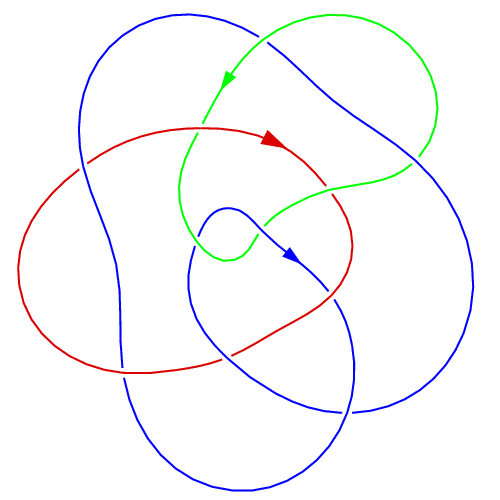
\includegraphics[width=\linewidth]{../data/link_mirror.png}
            \subcaption{lustro $mL$}
        \end{minipage}
        \begin{minipage}[b]{.32\linewidth}
            \centering
            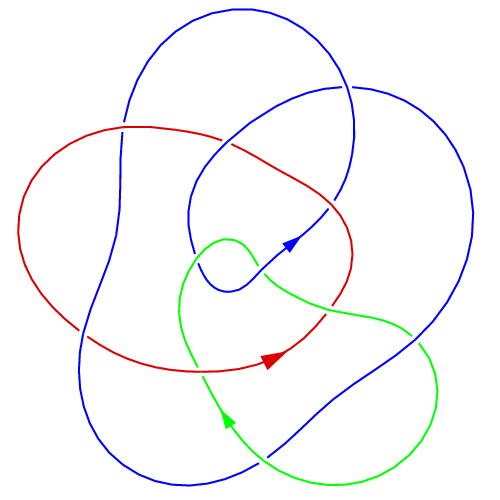
\includegraphics[width=\linewidth]{../data/link.png}
            \subcaption{przykładowy splot $L$}
        \end{minipage}
        \begin{minipage}[b]{.32\linewidth}
            \centering
            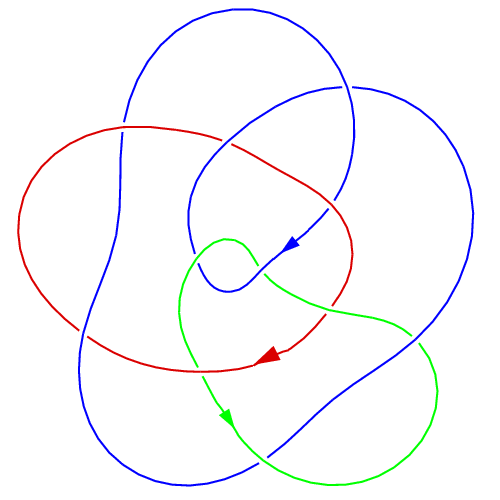
\includegraphics[width=\linewidth]{../data/link_reverse.png}
            \subcaption{rewers $rL$}
        \end{minipage}
    \end{figure}
\end{definition}

Na lewym obrazku odbiliśmy diagram względem poziomej prostej,
ale równie dobrze można po prostu zamienić każde nadskrzyżowanie na podskrzyżowanie.
Zauważmy, że wykonując powyższe operacje na węźle możemy otrzymać mniej niż czterech różne obiekty
($L$, $mL$, $rL$, $mrL$) -- na przykład trójlistnik jest własnym rewersem, ale nie lustrem.

\begin{definition}
    \index{węzeł!chiralny}
    \index{węzeł!odwracalny}
    \index{węzeł!zwierciadlany}
    Istnieje pięć typów symetrii węzłów:
    całkowicie chiralny albo skrętny (węzły $K$, $rK$, $mK$ są parami nierównoważne),
    odwracalny ($K \cong rK$),
    zwierciadlany ujemnie ($K \cong mrK$),
    zwierciadlany dodatnio ($K \cong mK$) oraz
    całkowicie zwierciadlany ($rK \cong K \cong mK$).
\end{definition}

Węzeł $9_{32}$ jest całkowicie skrętny.
Ósemka jest zwierciadlana, trójlistnik jest odwracalny,
zaś $8_{17}$ to najprostszy przykład węzła nieodwracalnego.
Ten ostatni fakt jest jednak daleki od oczywistego --
sześćdziesiąt lat temu nie było pewne,
czy węzły nieodwracalne w~ogóle istnieją.
W roku 1962 Ralph Fox wskazał kilku kandydatów do tego tytułu.
Hale Trotter odkrył rok później nieskończoną rodzinę nieodwracalnych precli (patrz \ref{def:pretzel}).
Obecnie wiadomo, że prawie wszystkie węzły są nieodwracalne (\cite[s.~46]{murasugi96}).
Wszystkie węzły torusowe są skrętne.

\begin{proposition}[Trotter, 1963] \label{trotter}
    Precel $(p, q, r)$, gdzie $p, q, r$ są parami różnymi liczbami całkowitymi, nie jest odwracalny.
\end{proposition}

\begin{proof}
    Praca \cite{trotter63} sprowadza w~elementarny sposób problem do pytania, czy pewna grupa posiada inwersję.
\end{proof}

Tait odnosił wrażenie, że zwierciadlane węzły mają parzysty indeks skrzyżowań,
ale Hoste (Thistlethwaite?) znalazł w~1998 kontrprzykład o~piętnastu skrzyżowaniach.
Jest on jedynym znanym nam dzisiaj.
Hipoteza Taita jest prawdziwa dla węzłów pierwszych, alternujących.

Poniższa tabela oparta jest (kolejno) o~ciągi
\href{https://oeis.org/A051766}{51766},
\href{https://oeis.org/A051769}{51769},
\href{https://oeis.org/A051768}{51768},
\href{https://oeis.org/A051767}{51767},
\href{https://oeis.org/A052400}{52400},
z bazy danych ``The On-Line Encyclopedia of Integer Sequences'' (OEIS).

\begin{table}[h]
    \centering
    \begin{tabular}{@{}*{20}l@{}} \toprule
        skrzyżowania & 3 & 4 & 5 & 6 & 7 & 8 & 9 & 10 & 11 & 12 & 13 & 14 \\ \midrule
        całkowicie skrętne & 0 & 0 & 0 & 0 & 0 & 0 & 2 & 27 & 187 & 1103 & 6919 & 37885 \\
        odwracalne & 1 & 0 & 2 & 2 & 7 & 16 & 47 & 125 & 365 & 1015 & 3069 & 8813 \\
        $-$ zwierciadlane & 0 & 0 & 0 & 0 & 0 & 1 & 0 & 6 & 0 & 40 & 0 & 227 \\
        $+$ zwierciadlane & 0 & 0 & 0 & 0 & 0 & 0 & 0 & 0 & 0 & 1 & 0 & 6 \\
        zwierciadlane & 0 & 1 & 0 & 1 & 0 & 4 & 0 & 7 & 0 & 17 & 0 & 41 \\
        \bottomrule
        \hline
    \end{tabular}
    \caption{Liczba węzłów o~poszczególnych typach symetrii}
    \label{tablica_wezlow}
\end{table}

Można wyróżnić jeszcze jeden rodzaj symetrii.

\begin{definition} \label{def_period}
    \index{węzeł!okresowy}
    Węzeł $K$ nazywamy $n$-okresowym, jeśli istnieje obrót $f \colon \R^3 \to \R^3$ o~kąt $2\pi/n$ wokół pewnej prostej $l$, rozłącznej z~węzłem, taki że $f(K) = K$.
\end{definition}

Trójlistnik jest 3-okresowy, węzeł $5_1$ 5-okresowy (widać to na standardowym diagramie) i~2-okresowy.
Tę drugą symetrię można dostrzec na diagramie realizującym indeks mostowy.

\begin{proposition}
    Zbiór wszystkich okresów jest niezmiennikiem węzłów.
\end{proposition}

Z~każdym węzłem okresowym związany jest inny, prostszy węzeł.
Niech $f$ będzie obrotem z definicji \ref{def_period}, zaś $p \colon \R^3 \to \R^3/f \simeq \R^3$ rzutem na przestrzeń ilorazową.
\index{węzeł!ilorazowy}
Wtedy $p(K)$ nazywamy \emph{węzłem ilorazowym}, zaś $K$ to jego $n$-krotne nakrycie.

Murasugi podał dwa warunki, które musi spełniać węzeł o~okresie $n = p^r$, gdzie $r$ jest liczbą pierwszą.
Do ich zrozumienia potrzebujemy prostej definicji.
Ustalmy półprostą, która nie jest styczna do węzła $K$, po czym zorientujmy ją oraz węzeł.
Indeksem zaczepienia $\lambda$ węzła $p(K)$ jest różnica między liczbą skrzyżowań dodatnich oraz ujemnych wzdłuż półprostej (bez znaku).

\begin{proposition}[warunek Murasugiego]
    \index{warunek Murasugiego}
    Niech $K$ będzie węzłem o~okresie $n = p^r$, gdzie $p$ jest liczbą pierwszą.
    Niech $J$ będzie jego węzłem ilorazowym, z~indeksem zaczepienia $\lambda$.
    Wtedy wielomian $\Delta_J$ jest dzielnikiem wielomianu $\Delta_K$ oraz istnieje pewna całkowita liczba $k$, taka że
    \[
        \Delta_K = \pm \Delta_J^n \left(1 + t + t^2 + \ldots + t^{\lambda - 1}\right)^{n-1} \mod p.
    \]
\end{proposition}

Dowód to, jak zwykle, mozolne operacje na macierzach.

% Koniec podsekcji Lustro i~rewers

\subsection{Suma niespójna i~suma spójna} % (fold)
\label{sub:knot_sum}
Suma spójna węzłów to szczególny przypadek sklejenia dwóch rozmaitości wzdłuż brzegu.

\begin{definition}
    \index{suma!niespójna}
    Niech $L_1, L_2$ będą splotami.
    Ich \textbf{sumą niespójną}, $L_1 \sqcup L_2$,
    jest teoriomnogościowa suma rozłączna splotów
    $L_1$ i~$L_2$ leżących po różnych stronach pewnej płaszczyzny.
\end{definition}

\begin{definition}
    \index{suma!spójna}
    Nacinając dwa zorientowane węzły w~dwóch bliskich punktach i
    ponownie zszywając je dwoma łukami nieprzecinającymi już
    istniejących otrzymujemy \textbf{sumę spójną}, $K_1 \shrap K_2$.
    \[
        \begin{tikzpicture}[baseline=-0.65ex,scale=0.1]
        \begin{knot}[clip width=5, flip crossing/.list={5}, ignore endpoint intersections=false,]
            \strand[thick] (-3.5, -3.5) [in=down, out=up] to (3.5, 3.5);
            \strand[thick] (3.5, 3.5) [in=right, out=up] to (-4.5, 10);
            \strand[thick] (-4.5, 10) [in=up, out=left] to (-10, 3.5);
            \strand[thick] (-10, 3.5) to (-10, -3.5);
            \strand[thick] (-10, -3.5) [in=left, out=down] to (-4.5, -10);
            \strand[thick] (-4.5, -10) [in=down, out=right] to (3.5, -3.5);
            \strand[thick] (3.5, -3.5) [in=down, out=up] to (-3.5, 3.5);
            \strand[thick] (-3.5, 3.5) [in=left, out=up] to (4.5, 10);
            \strand[thick] (4.5, 10) [in=up, out=right] to (10, 3.5);
            \strand[thick, -Latex] (10, 3.5) to (10, -3.5);
            \strand[thick] (10, -3.5) [in=right, out=down] to (4.5, -10);
            \strand[thick] (4.5, -10) [in=down, out=left] to (-3.5, -3.5);
            \node at (0, -15) {$K_1$};
        \end{knot}
        \end{tikzpicture}
        \shrap
        \begin{tikzpicture}[baseline=-0.65ex,scale=0.1]
        \begin{knot}[clip width=5, flip crossing/.list={6}, ignore endpoint intersections=false,]
            \strand[thick] (-3.5, -3.5) [in=down, out=up] to (3.5, 3.5);
            %\strand[thick] (3.5, 3.5) [in=right, out=up] to (-4.5, 10);
            %\strand[thick] (-4.5, 10) [in=up, out=left] to (-10, 3.5);
            \strand[thick] (-10, -3.5) [in=left, out=up] to (0, 6.5);
            \strand[thick, Latex-] (-10, -3.5) [in=left, out=down] to (-4.5, -10);
            \strand[thick] (-4.5, -10) [in=down, out=right] to (3.5, -3.5);
            \strand[thick] (3.5, -3.5) [in=down, out=up] to (-3.5, 3.5);
            %\strand[thick] (-3.5, 3.5) [in=left, out=up] to (4.5, 10);
            %\strand[thick] (4.5, 10) [in=up, out=right] to (10, 3.5);
            \strand[thick] (10, -3.5) [in=right, out=up] to (0, 6.5);
            \strand[thick] (10, -3.5) [in=right, out=down] to (4.5, -10);
            \strand[thick] (4.5, -10) [in=down, out=left] to (-3.5, -3.5);
            %
            \strand[thick] (-3.5, 3.5) [in=left, out=up] to (0, 10);
            \strand[thick] (3.5, 3.5) [in=right, out=up] to (0, 10);
            \node at (0, -15) {$K_2$};
        \end{knot}
        \end{tikzpicture}
        =
        \begin{tikzpicture}[baseline=-0.65ex,scale=0.1]
        \begin{knot}[clip width=5, flip crossing/.list={5, 22, 23}, ignore endpoint intersections=false,]
            \strand[thick] (-18.5, -3.5) [in=down, out=up] to (-11.5, 3.5);
            \strand[thick] (-11.5, 3.5) [in=right, out=up] to (-19.5, 10);
            \strand[thick] (-19.5, 10) [in=up, out=left] to (-25, 3.5);
            \strand[thick] (-25, 3.5) to (-25, -3.5);
            \strand[thick] (-25, -3.5) [in=left, out=down] to (-19.5, -10);
            \strand[thick] (-19.5, -10) [in=down, out=right] to (-11.5, -3.5);
            \strand[thick] (-11.5, -3.5) [in=down, out=up] to (-18.5, 3.5);
            \strand[thick] (-18.5, 3.5) [in=left, out=up] to (-10.5, 10);
            \strand[thick] (-10.5, 10) [in=left, out=right] to (-5, 2);
            \strand[thick, -Latex] (-5, 2) to (-5+6, 2);
            \strand[thick] (5, 2) to (-5+6, 2);
            \strand[thick] (3, -2) to [in=left, out=right] (10.5, -10);
            \strand[thick, -Latex] (3, -2) to (0, -2);
            \strand[thick] (-5, -2) to (0, -2);
            \strand[thick] (-5, -2) [in=right, out=left] to (-10.5, -10);
            \strand[thick] (-10.5, -10) [in=down, out=left] to (-18.5, -3.5);
            %%%
            \strand[thick] (11.5, -3.5) [in=down, out=up] to (18.5, 3.5);
            \strand[thick] (-10 +15, 2) [in=left, out=right] to (15, 6.5);
            \strand[thick] (10.5, -10) [in=down, out=right] to (18.5, -3.5);
            \strand[thick] (18.5, -3.5) [in=down, out=up] to (11.5, 3.5);
            \strand[thick] (25, -3.5) [in=right, out=up] to (15, 6.5);
            \strand[thick] (25, -3.5) [in=right, out=down] to (19.5, -10);
            \strand[thick] (19.5, -10) [in=down, out=left] to (11.5, -3.5);
            \strand[thick] (11.5, 3.5) [in=left, out=up] to (15, 10);
            \strand[thick] (18.5, 3.5) [in=right, out=up] to (15, 10);
            %%%
            \node at (0, -15) {$K_1 \shrap K_2$};
        \end{knot}
        \end{tikzpicture}
        \]
\end{definition}

Uogólnieniem tego działania oraz
(nieopisanej w~naszej pracy) operacji \emph{plumbing}
jest suma Murasugiego, dobrze wyjaśniona w~czwartym rozdziale \cite{kawauchi96}.

Ważna jest orientacja składników:
suma dwóch trójlistników może być,
w zależności od ich orientacji,
węzłem babskim\footnote{Nazewnictwo pochodzi od żeglarzy, nie matematyków. Z angielskiego \emph{granny knot}, \emph{square knot}.} lub prostym.
Fox pokazał w~1952 roku,
że dopełnienia tych dwóch węzłów nie są homeomorficzne.
Suma przeciwnie skręconych trójlistników jest plastrowa
(definicja \ref{def:slice_knot}),
natomiast tak samo skręconych -- nie.

\begin{proposition}
    Suma spójna jest dobrze określonym działaniem.
\end{proposition}

Suma spójna nie jest dobrze określona dla splotów:
nie istnieje kanoniczny wybór, które składowe łączyć ze sobą.

\begin{proof}
    Niech dane będą węzły $K_1$ oraz $K_2$
    oraz dwa różne łuki $\gamma_1$, $\gamma_2$,
    których można użyć do konstrukcji sumy spójnej.
    Skurczmy $K_1$, przeciągnijmy najpierw przez łuk $\gamma_1$, a~następnie wzdłuż węzła $K_2$.
    Teraz wystarczy odwrócić ten proces z~$\gamma_2$ w~miejscu $\gamma_1$.
\end{proof}

\begin{proposition}
    Suma spójna zorientowanych węzłów posiada następujące własności:
    \begin{enumerate}[leftmargin=*]
    \itemsep0em
        \item jest łączna:
        $(K_1 \shrap K_2) \shrap K_3 \simeq K_1 \shrap (K_2 \shrap K_3)$,
        \item jest przemienna:
        $K_1 \shrap K_2 \simeq K_2 \shrap K_1$,
        \item posiada element neutralny:
        $K_1 \shrap \LittleUnknot \simeq \LittleUnknot \shrap K_1 \simeq K_1$.
    \end{enumerate}
\end{proposition}

Prosty dowód tego faktu pozostawiamy Czytelnikowi.
Pokażemy za to, iż węzły z~sumą spójną nie tworzą grupy -- brakuje elementów przeciwnych.

\begin{proposition}
    Jeśli $K \shrap L = \Unknot$, to $K = L = \Unknot$.
\end{proposition}

\begin{proof}[Niedowód]
    Technika ta zwana jest szwindlem Mazura.
    Załóżmy, że $K \shrap L = \Unknot$ i~dopuśćmy wyjątkowo węzły dzikie.
    Skonstruujmy sumę $K \shrap L \shrap K \shrap \ldots$,
    przy czym kolejne składniki powinny zmniejszać się,
    aby ich suma nadal była węzłem.
    Wtedy
    \begin{align*}
        K & \simeq K \shrap [(L \shrap K) \shrap (L \shrap K) \ldots] \\
         & \simeq (K \shrap L) \shrap (K \shrap L) \shrap \ldots
         \simeq \Unknot \shrap \Unknot \shrap \ldots
         \simeq \Unknot.
    \end{align*}
    Analogicznie pokazujemy, że $L \simeq \Unknot$.
\end{proof}

Później poznamy prawdziwy, oparty na topologii algebraicznej, dowód.
Połączymy fakty \ref{genus_one} oraz \ref{genus_sum}.

Półgrupę węzłów z~operacją sumy spójnej można ulepszyć do grupy na dwa sposoby:
albo poprzez zmianę działania, w~jakie jest wyposażona,
albo osłabiając definicję węzłów równoważnych.
Drugi pomysł jest dużo lepszy niż pierwszy.
Na początku lat pięćdziesiątych J. Milnor wprowadził do matematyki pojęcie zgodności
(z angielskiego \emph{concordance}), które zastąpiło zwykłą równoważność.
Element neutralny nowej grupy to węzły plastrowe, ich opis leży w~sekcji \ref{sec:slice}.
Zagadnienia te zakorzenione są w~czterowymiarowej topologii.

% Koniec podsekcji Suma niespójna i~suma spójna

% Koniec sekcji Operacje na węzłach

\section{Węzły pierwsze}
\label{sec:prime_knots}
Istnieje węzłowy odpowiednik liczb pierwszych.
Jest on ściśle związany z podaną wyżej operacją sumy spójnej.
Do jego dostatecznie dobrego zrozumienia wymagana jest znajomość powierzchni Seiferta (opisanych w sekcji \ref{sec:genus}).

\begin{definition} \label{primeknot}
    Nietrywialny węzeł nazywamy \textbf{pierwszym},
    kiedy nie można przedstawić go jako sumy spójnej $K_1 \shrap K_2$
    dwóch nietrywialnych węzłów $K_1, K_2$ (nie jest złożony).
\end{definition}

Okazuje się, że jeśli alternujący \todo{definicja splotów alternujących} splot nie jest pierwszy,
to każdy jego alternujący diagram jest złożony.
Jako pierwszy fakt ten został wykazany przez Menasco w \cite{menasco84}.
Dowód opiera się na multiplikatywności wielomianu BLM/Ho (opisuje go definicja \ref{def:blm_ho}).

Czy węzłów pierwszych jest nieskończenie wiele?
Tak (patrz fakt \ref{infty_primes}), potrafimy nawet oszacować ich liczbę.
W roku 1987 C. Ernst, D. Sumners w oparciu o wyniki Thistlethwaite'a, Kauffmana, oraz Murasugiego dotyczące węzłów alternujących pokazali w \cite{ernst87},
że różnych węzłów pierwszych o $n$ skrzyżowaniach jest co najmniej $\frac 1 3 (2^{n- 2} - 1)$ dla $n \ge 4$,
przy czym węzły lustrzane traktowane są jako różne.
Welsh znalazł ograniczenie
\[
    \limsup_{n \to \infty} \sqrt[n]{N(n)} \le 13.5,
\]
gdzie $N(n)$ jest ilością pierwszych węzłów o $n$ skrzyżowaniach.

Czy niewęzeł nie daje się zapisać jako suma dwóch innych węzłów?
Byłoby to skrajnie niepożądane, gdyż każdy węzeł jest naturalnie spójną sumą siebie oraz niewęzła.
Na szczęście przy pomocy powierzchni Seiferta można pokazać, że tak się nie dzieje (jest to wniosek \ref{no_inverses}).
Prawdziwe jest dużo mocniejsze stwierdzenie,
którego nie udowodnimy ze względu na niedostatecznie rozwinięty aparat matematyczny.
Należy o nim myśleć jak o analogonie zasadniczego twierdzenia arytmetyki.

\begin{theorem}[Schubert, 1949]
    Każdy różny od niewęzła węzeł rozkłada się jednoznacznie na węzły pierwsze
    (jeśli tylko pominąć kolejność składników).
\end{theorem}

Pomimo to uda się nam pokazać samo istnienie rozkładu, jest to fakt \ref{genus_sum}.
% koniec sekcji Węzły pierwsze

\section{Niezmienniki liczbowe}
Jak wspomnieliśmy na początku rozdziału, sprawdzenie,
czy dwa diagramy przedstawiają sploty równoważne,
jest uciążliwym i czasochłonnym zadaniem.
Aby je uprościć, podamy opis kilku prostych niezmienników o całkowitych wartościach.
Zachodzą implikacje:
sploty równoważne $\Rightarrow$ ta sama wartość niezmiennika
oraz różne wartości niezmiennika $\Rightarrow$ różne sploty.

\subsection{Indeks skrzyżowaniowy} % (fold)
\label{sub:crossing_number}
Z angielskiego \emph{crossing number}.

\begin{definition}
    Indeks skrzyżowaniowy $\operatorname{cr}(L)$ splotu $L$ to
    minimalna liczba skrzyżowań widocznych na diagramie,
    który przedstawia splot $L$.
\end{definition}

Wciąż nie jest wiadome, czy indeks skrzyżowaniowy jest addytywny względem sumy spójnej.
Potrafimy to jednak udowodnić dla niektórych węzłów: alternujących, adekwatnych czy torusowych.
Lackenby w pracy \cite{lackenby09} pokazał, że dla pewnej stałej $N > 1$ zachodzi
\[
    \operatorname{cr} L_1 + \operatorname{cr} L_2 \le N \cdot \operatorname{cr} (L_1 \# L_2).
\]
Jego podejście (przez powierzchnie normalne) nie jest w stanie poprawić stałej do $N = 1$.

% Koniec podsekcji Indeks skrzyżowaniowy

\subsection{Liczba gordyjska} % (fold)
\label{sub:unknotting_number}
Z angielskiego \emph{unknotting number}.

\begin{definition}
    Liczba gordyjska $\operatorname{u}(K)$ węzła $K$ to minimalna liczba skrzyżowań,
    które trzeba odwrócić na pewnym jego diagramie, by dostać niewęzeł.
    Liczba $u$ nie musi być osiągana przez diagram o minimalnej liczbie skrzyżowań.
\end{definition}

Dotychczas wyznaczono liczbę gordyjską dla prawie wszystkich węzłów pierwszych o co najwyżej dziesięciu skrzyżowaniach,
Cha i Livingston podają następującą listę wyjątków: 
$10_{11}$, $10_{47}$, $10_{51}$, $10_{54}$, $10_{61}$, $10_{76}$, $10_{77}$, $10_{79}$, $10_{100}$ (stan na rok 2008).
S. Bleiler odkrył w \cite{bleiler84} fascynujący przykład wymiernego węzła $2$-gordyjskiego,
czego świadkiem nie może być diagram o minimalnej liczbie skrzyżowań
(ponieważ, co jeszcze bardziej fascynujące, węzeł ten posiada tylko jeden diagram o dziesięciu skrzyżowaniach z trzema do odwrócenia).
Koduje go liczba $29/6$, w tabeli węzłów figuruje jako $10_8$.
Stoimenow w \cite{stoimenow01} pokazuje, że jeden węzeł może mieć kilka diagramów minimalnych,
z których tylko niektóre są świadkiem $1$-gordyjskości (są to między innymi $14_{36750}$ oraz $14_{36760}$.)

Jeśli odwrócenie pewnych skrzyżowań daje niewęzeł, to odwrócenie pozostałych także.
To daje proste, choć niezbyt pomocne oszacowanie liczby gordyjskiej: $2 \operatorname{u} (K) \le \operatorname{cr} (K)$. 
Borodzik oraz Friedl podali niedawno całkiem mocne ograniczenia na liczbę gordyjską w pracach \cite{borodzik14} i \cite{borodzik15} opierając się o parowanie Blanchfielda
(poprawiając ograniczenia z sygnatury Levine'a-Tristrama, indeksu Nakanishiego oraz przeszkodą Lickorisha).
Dwadzieścia pięć węzłów o co najwyżej dwunastu skrzyżowaniach ma liczbę gordyjską równą co najmniej trzy, co trudno pokazać innymi metodami.

Dla każdego nietrywialnego splotu istnieje diagram wymagający odwrócenia  dowolnie wielu skrzyżowań (dowód zawiera praca \cite{taniyama09} Taniyamy).
Pokazany jest tam jeszcze jeden godny uwagi fakt.
Jeśli liczba gordyjska diagramu $D$ wynosi $\frac 12 (c(D) - 1)$,
co jest maksymalną możliwą wartością zgodnie z naszym prostym ograniczeniem,
to węzeł jest $(2,p)$-torusowy albo wygląda jak diagram niewęzła po pierwszym ruchu Reidemeistera.

% Liczba gordyjska nietrywialnego węzła skręconego (definicja \ref{twist_knots}) to jeden, wystarczy bowiem rozwiązać jego splecione końce.
Patrz także stwierdzenie \ref{torus_unknotting}.

Od początku teorii węzłów podejrzewano, że liczba gordyjska jest addytywna, to znaczy $u(K \shrap J) = u(K) + u(J)$.
Z tej nieudowodnionej do dzisiaj hipotezy można wyciągnąć wniosek,
że jeśli do rozwiązania węzła wystarcza odwrócenie skrzyżowania, to jest pierwszy.
Podejrzewał to H. Wendt w 1937 roku,
kiedy policzył liczbę gordyjską węzła babskiego używając homologii rozgałęzionego nakrycia cyklicznego.

\begin{proposition}
    Węzły $1$-gordyjskie są pierwsze.
\end{proposition}

\begin{proof}[Niedowód]
    W pracy \cite{scharleman85} z 1985 roku M. Scharleman podał dość zawiłe uzasadnienie, w które zamieszane były grafy planarne.
\end{proof}

W pracy \cite{shimizu14} Ayaka Shimizu pokazuje przykład innej operacji rozwiązującej węzły, ale nie sploty:
zmianę skrzyżowań wokół obszaru na diagramie.

Przestrzeń gordyjska
(wszystkich węzłów wyposażona w metrykę pochodzącą od liczby gordyjskiej)
bywa sprzeczna z intuicją.
W pracy ,,Braids and signatures'' J. Gambaudo, E. Ghys (twierdzenie C) pokazali,
że przestrzeń węzłów zawiera prawie idalną kopię przestrzeni euklidesowej dowolnego wymiaru.
Dokładniej:

\begin{proposition}
    Dla każdej liczby całkowitej $d \ge 1$ istnieje funkcja $\xi: \Z^d \to \mathcal{K}$, która dla pewnych stałych $A, B, C \ge 0$ i pewnej normy $\|\cdot\|$ spełnia podwójną nierówność
    \[
        A\|x-y\|  - B \le d(\xi(x), \xi(y)) \le C\|x-y\|.
    \]
\end{proposition}

% Koniec podsekcji Liczba gordyjska

\subsection{Liczba mostowa} % (fold)
\label{sub:bridge_index}
Z angielskiego \emph{bridge number}.
Wprowadzona w 1954 przez Schuberta.
\begin{definition}
    Liczba mostowa $\operatorname{br}(K)$ to minimalna liczba mostów:
    długich łuków, które biegną przez nadskrzyżowania.
\end{definition}

Można pokazać, że $n$-mostowe węzły rozkładają się na sumę dwóch trywialnych $n$-supłów.

\begin{proposition}
    Niech $K_1, K_2$ będą węzłami.
    Wtedy $\operatorname{br} (K_1) + \operatorname{br}(K_2) = \operatorname{br}(K_1 \# K_2) + 1$.
\end{proposition}

\begin{proof}
    Schultens w artykule \cite{schultens03} dowodzi (przy użyciu foliacji na brzegu węzła towarzysza w satelitarnym) jeszcze raz tego, co pokazał Schubert w \cite{schubert54}.
    Z tego względu nie możemy tutaj opowiedzieć o szczegółach technicznych dowodu.
\end{proof}

Tylko jeden węzeł jest jednomostowy, to niewęzęł.
Kolejne w hierarchi skomplikowania, czyli dwumostowe,
to domknięcia wymiernych supłów, patrz fakt \ref{two_bridge_tangle}.
Węzły trójmostowe pozostają nie do końca zbadane.

\todo[inline]{Hipoteza mówi, że $c \ge 3 br - 3$, z równością dla inewęzła i sum trójlistników.}

% Koniec podsekcji Liczba mostowa

\subsection{Liczba warkoczowa} % (fold)
\label{sub:braid_number}
Z angielskiego \emph{braid number}.
Do jej określenia potrzebna jest definicja \ref{braid_def}.

\begin{definition}
    Liczba warkoczowa to minimalna liczba pasm, na których można zbudować warkocz, którego domknięciem jest wyjściowy węzeł.
\end{definition}

\begin{proposition}
    Węzeł o $n$ skrzyżowaniach można zapleść na $n - 1$ pasmach.
\end{proposition}

Indeks warkoczowy zależy od orientacji ogniw i trudno się go wyznacza w ogólnym przypadku.
Poniższy dowód zakłada znajomość warkoczy (rozdział piąty).

\begin{proposition}
    Indeksem warkoczowym węzła torusowego $K(q, r)$, $rq \neq 0$, jest $\min\{|q|, |r|\}$.
\end{proposition}

\begin{proof}
Niech $K$ będzie węzłem torusowym typu $(q,r)$ z minimalnym przedstawieniem jako warkocz $\beta$.
Z konstrukcji domknięcia (czyli dołączenia rozłącznych półokręgów) wynika, 
że diagram $K$ ma dokładnie $b(K)$ lokalnych maksimów.
Definicja indeksu mostowego orzeka, iż $br(K) \le b(K)$.
Bez straty ogólności niech $q > r > 0$.
Skoro węzeł $K$ powstaje z $r$-warkocza $(\sigma_{r-1} \ldots \sigma_2\sigma_1)^q$, 
indeks $b(K)$ nie przekracza $r = br(K)$.

Skorzystaliśmy z faktu \ref{torus_bridge}.
\end{proof} 

% Koniec podsekcji Liczba warkoczowa

\subsection{Indeks zaczepienia} % (fold)
\label{sub:linking_number}
\begin{definition} \label{sign_def}
    Na diagramie zorientowanego splotu, każdemu skrzyżowaniu przypisujemy \textbf{znak} równy $\pm 1$.
    Skrzyżowania dodatnie nazywamy praworęcznymi, ujemne zaś: leworęcznymi.
    \[
        \sign \Bigl(\,\,\begin{tikzpicture}[baseline=-0.65ex,scale=0.07]
        \begin{knot}[clip width=5]
        \strand[semithick,-Latex] (-5,-5) -- (5,5);
        \strand[semithick,Latex-] (-5,5) -- (5,-5);
        \end{knot}\end{tikzpicture}\,\,\Bigr) = +1 \quad
        \sign \Bigl(\,\,\begin{tikzpicture}[baseline=-0.65ex,scale=0.07]
        \begin{knot}[clip width=5, flip crossing/.list={1}]
        \strand[semithick,-Latex] (-5,-5) -- (5,5);
        \strand[semithick,Latex-] (-5,5) -- (5,-5);
        \end{knot}\end{tikzpicture}\,\,\Bigr) = -1
    \]
    \textbf{Indeks zaczepienia} splotu zorientowanego $L$ o diagramie $D$ to $\frac 12 \sum_c \sign (c)$,
    gdzie $c$ przebiega każde skrzyżowanie, przy którym spotykają się \emph{różne} składowe.
    Oznaczenie: $\operatorname{lk}(L)$.
\end{definition}

Zauważmy, że indeks zaczepienia splotu Hopfa wynosi $1$, natomiast splotu Whiteheada $0$.
Są więc istotnie różne.

\begin{proposition}
    Indeks zaczepienia jest dobrze określonym niezmiennikiem zorientowanych węzłów.
\end{proposition}

\begin{proof}
    Sprawdźmy wpływ ruchów Reidemeistera na wartość
    $\operatorname{lk}(L)$:

    \[
        \fbox{
        \begin{tikzpicture}[baseline=-0.65ex,scale=0.07]
        \begin{knot}[clip width=5]
        \strand[semithick] (-10,10) .. controls (-10,2) and (-10,2) .. (-6,-2);
        \strand[semithick] (-10,-10) .. controls (-10,-2) and (-10,-1) .. (-9,0);
        \strand[semithick] (-7,1) -- (-6,2);
        \strand[semithick] (-6,2) .. controls (2,9) and (2,-9) .. (-6,-2);
        \end{knot}
        \end{tikzpicture}
        $\stackrel{R_1}{\cong} \,\,$
        \begin{tikzpicture}[baseline=-0.65ex,scale=0.07]
        \begin{knot}[clip width=5]
        \strand[semithick] (0,10) -- (0,-10);
        \end{knot}
        \end{tikzpicture}}
        %%%
        \quad \fbox{
        \begin{tikzpicture}[baseline=-0.65ex,scale=0.07]
        \begin{knot}[clip width=5]
        \strand[semithick] (4,-10) .. controls (4,-4) and (-4,-4) .. (-4,0);
        \strand[semithick] (4,10) .. controls (4, 4) and (-4, 4) .. (-4,0);
        \strand[semithick] (-4,-10) .. controls (-4,-4) and (4,-4) .. (4,0);
        \strand[semithick] (-4,10) .. controls (-4, 4) and (4,4) .. (4,0);
        \node[blue] at (-4,4)[left] {$a$};
        \node[blue] at (-4,-4)[left] {$-a$};
        \end{knot}
        \end{tikzpicture}
        $\stackrel{R_2}{\cong} \,\,$
        \begin{tikzpicture}[baseline=-0.65ex,scale=0.07]
        \begin{knot}[clip width=5]
        \strand[semithick] (4,-10) .. controls (4,-4) and (1,-4) .. (1,0);
        \strand[semithick] (4,10) .. controls (4, 4) and (1, 4) .. (1,0);
        \strand[semithick] (-4,-10) .. controls (-4,-4) and (-1,-4) .. (-1,0);
        \strand[semithick] (-4,10) .. controls (-4, 4) and (-1,4) .. (-1,0);
        \end{knot}
        \end{tikzpicture}}
        %%%
        \quad \fbox{
        \begin{tikzpicture}[baseline=-0.65ex,scale=0.07]
        \begin{knot}[clip width=5, flip crossing/.list={1,2,3}]
        \strand[semithick] (-10,-10) -- (10,10);
        \strand[semithick] (-10,10) -- (10,-10);
        \strand[semithick] (-10,-2) .. controls (-4, -2) and (-4,8) .. (0,8);
        \strand[semithick] (10,-2) .. controls (4, -2) and (4,8) .. (0,8);
        \node[blue] at (-6,4)[left] {$a$};
        \node[blue] at (6,4)[right] {$b$};
        \node[blue] at (0,-2)[below] {$c$};
        \end{knot}
        \end{tikzpicture}
        $\stackrel{R_3}{\cong} \,\,$
        \begin{tikzpicture}[baseline=-0.65ex,scale=0.07]
        \begin{knot}[clip width=5, flip crossing/.list={1,2,3}]
        \strand[semithick] (-10,-10) -- (10,10);
        \strand[semithick] (-10,10) -- (10,-10);
        \strand[semithick] (-10,2) .. controls (-4, 2) and (-4,-8) .. (0,-8);
        \strand[semithick] (10,2) .. controls (4, 2) and (4,-8) .. (0,-8);
        \node[blue] at (-6,-4)[left] {$a$};
        \node[blue] at (6,-4)[right] {$b$};
        \node[blue] at (0,2)[above] {$c$};
        \end{knot}
        \end{tikzpicture}}
    \]
    Na mocy twierdzenia Reidemeistera dowód został zakończony.
\end{proof}

\todo[inline]{Linking number jest zawsze całkowita (tw. Jordana)}

% Koniec podsekcji Indeks zaczepienia

\subsection{Sygnatura} % (fold)
\label{sub:signature}
Sygnatura pojawia się w fakcie \ref{slice_signature}.

\begin{definition}
    Sygnatura to niezmiennik topologiczny zadany (kłębiastą) relacją rekurencyjną:
    \begin{itemize}[leftmargin=*]
    \itemsep0em
        \item $\sigma (\MalyNieWezel) = 0$,
        \item $\sigma (K_+) - \sigma (K_-) \in \{0, 2\}$,
        \item $4 \mid \sigma (K)$ wtedy i tylko wtedy, gdy $\nabla(2i) > 0$ (wielomian Conwaya).
    \end{itemize}
\end{definition}

Sygnatura pozwala uzyskać proste oszacowanie liczby gordyjskiej od dołu:

\begin{proposition}
    Mamy $2 u(K) \ge |\sigma(K)|$.
\end{proposition}

Nie istnieje bezpośredni związek między sygnaturą i liczbą mostową.
Węzeł torusowy $T_{2,n}$ jest dwumostowy, jego sygnatura wynosi $n - 1$.
Suma spójna węzłów prostych ma zerową sygnaturę i nieograniczoną liczbę mostową.

% Koniec podsekcji Sygnatura

% Koniec sekcji Niezmienniki liczbowe


\chapter{Niezmienniki kolorowe}
Sklasyfikowanie wszystkich węzłów jest nie jest jeszcze możliwe, dlatego w tym rozdziale wyróżnimy pewne rodziny i ograniczymy rozważania do nich.

\section{Macierz i~wyznacznik} % (fold)
\label{sec:colour_matrix}
Zajmiemy się teraz wyznacznikiem, pierwszym nieoczywistym niezmiennikiem splotów, który przypisuje każdemu pewną liczbę całkowitą.
Jest on blisko związany z~kolorowaniem.
Zauważmy, że pierwszy ruch Reidemeistera usuwa zamknięte krzywe, czyli pojedyncze łuki bez skrzyżowań.
Diagram bez takich krzywych ma tyle samo skrzyżowań, co łuków.

\begin{definition}[macierz kolorująca]
    \index{macierz!kolorująca}
    Ustalmy diagram bez zamkniętych krzywych dla splotu $L$ z~łukami $x_0, \ldots, x_m$ oraz skrzyżowaniami $0, \ldots, m$.
    Definiujemy macierz $A$, której wyraz $a_{lj}$ jest współczynnikiem przy $x_j$ w~$l$-tym równaniu kolorującym: $x_j+x_k - 2x_i \equiv 0 \mod n$.
    Macierz kolorująca $A_+$ powstaje z~macierzy $A$ przez skreślenie dowolnego wiersza i~kolumny.
    \[\begin{tikzpicture}[baseline=-0.65ex, scale=0.12]
    \useasboundingbox (-5, -5) rectangle (5,5);
    \begin{knot}[clip width=5, end tolerance=1pt, flip crossing/.list={1}]
        \strand[semithick] (-5,5) to (5,-5);
        \strand[semithick] (-5,-5) to (5,5);
        \node[darkblue] at (5, 5)[below right] {$x_i$};
        \node[darkblue] at (5, -5)[above right] {$x_j$};
        \node[darkblue] at (-5, 5)[below left] {$x_k$};
    \end{knot}
    \end{tikzpicture}\]
\end{definition}

Taka macierz jest kwadratowa, ponieważ z~każdego skrzyżowania wychodzą (tunelem) dwa włókna mające dwa końce.
Wykreślenie wiersza i~kolumny jest konieczne.
Gdybyśmy tego zaniechali, otrzymana macierz nie byłaby odwracalna, bowiem wiersze sumują się do zera.
Dla alternujących diagramów możemy żądać, by górą $i$-tego skrzyżowania biegło $i$-te włókno, wtedy na diagonali macierzy $A$ znajdą się same minus dwójki.

\begin{definition}[wyznacznik]
    \index{wyznacznik}
    \label{def:determinant}
    Wyznacznik splotu różnego od niewęzła to wyznacznik jego macierzy kolorującej bez znaku.
    Wyznacznikiem niewęzła jest $1$.
\end{definition}

\begin{definition}[defekt]
    Defekt (wymiar jądra) macierzy kolorującej modulo $p$ nazywamy defektem węzła.
\end{definition}

Defekty modulo różne liczby pierwsze są niezależne od siebie.
Na przykład suma spójna $k$ trójlistników i~$j$ węzłów $T_{2,5}$ posiada defekt $k$ modulo $3$ oraz $j$ modulo $5$.
Podobne przykłady istnieją dla innych zbiorów liczb pierwszych.

Pokażemy później (po poznaniu grupy kolorującej, czyli we wniosku \ref{det_invariant}) lub jeszcze później (po wprowadzeniu wielomianu Alexandera, w~dowodzie faktu \ref{alexander_invariance}), że wyznacznik splotu jest dobrze określony: nie zależy on od wyboru etykietowania, minora macierzy oraz diagramu i~że jest niezmiennikiem.
Teraz ograniczymy się do jego kilku własności.

Defekt także jest niezmiennikiem, choć rzadziej używanym.
Węzeł o~defekcie $n$ modulo $p$ posiada $p(p^n-1)$ kolorowań $p$ kolorami.
Węzły $8_{18}$ oraz $9_{24}$ mają ten sam wyznacznik, $45$.
Ich defekty modulo $3$ to $1$ i~$2$, zatem są różne.

% Każde $p$-kolorowanie węzła $n$-mostowego jest wyznaczone przez kolory $n$ mostów
% % To brzmi podejrzanie: więc przestrzeń kolorowań ma wymiar co najwyżej $n$ i~defekt modulo $p$ nie przekracza $\operatorname{br} - 1$.
% Wnioskujemy stąd, że $(3,3,3)$-precel nie jest dwumostowy.

% \begin{proof}
%     \emph{Krok pierwszy}.
%     Pokażemy, że żaden ruch Reidemeistera nie zmienia wyznacznika.
%     \begin{enumerate}
%         \item \emph{Ruch $R_1$}. Diagram przed lub po ruchu zawiera co najmniej jedno włókno, które łączy tunel z~mostem pewnego skrzyżowania.
%         \item \emph{Ruch $R_2$}.
%         \item \emph{Ruch $R_3$}.
%     \end{enumerate}

%     \emph{Krok drugi}.
%     Niech $A_{i,j}$ oznacza minor powstały przez skreślenie $i$-tego wiersza oraz $j$-tej kolumny.
%     Pokażemy, że wartość wyznacznika nie zależy od wyboru $i$ oraz $j$.

%     Niech $X$ będzie macierzą $k \times k$ złożoną z~samych jedynek.
%     Suma elementów w~każdej kolumnie oraz każdym wierszu macierzy $A + X$ wynosi $k$, ponieważ znaki równań zostały dobrze wybrane.
%     Wykonujemy kolejno operacje:
%     \begin{enumerate}
%         \item Dodajemy do $i$-tego wiersza sumę pozostałych.
%         \item Dodajemy do $j$-tej kolumny sumę pozostałych.
%         Teraz $i$-ty wiersz oraz $j$-ta kolumna zawierają wyrazy $k$ z~wyjątkiem $a_{ij}$, który wynosi $k^2$.
%         \item Wyciągamy $k$ z~$i$-tego wiersza przed wyznacznik.
%         \item Odejmujemy $i$-ty wiersz od pozostałych.
%     \end{enumerate}
%     Rozwinięcie Laplace'a względem $j$-tej kolumny mówi, że $|\det (A+X)| = k^2 |(-1)^{i+j} \det A_{i,j}|$, co kończy dowód drugiego kroku.

%     \emph{Krok trzeci}.
%     Pokażemy, że zmiana etykietowania nie zmienia wyznacznika.
% \end{proof}

\begin{proposition}
    \label{prp:colour_det}
    Splot $L$ koloruje się modulo $n$ wtedy i~tylko wtedy, gdy liczby $\det L$ oraz $n$ nie są względnie pierwsze.
\end{proposition}

\begin{proof}
    Bez straty ogólności ograniczmy się do tych kolorowań, gdzie $x_0 = 0$.
    Kolorowanie modulo $n$ istnieje dokładnie wtedy, gdy istnieje niezerowy wektor $(x_1, x_2, \ldots, x_m)$ taki, że $Ax \equiv 0 \mod n$.
    Ale z~algebry liniowej wiemy, że dla pewnych całkowitoliczbowych macierzy $C, R$ macierz $RAC = diag(y_1, \ldots, y_m)$ jest diagonalna.
    Warunek z~faktu tłumaczy się wtedy na istnienie rozwiązania dla przynajmniej jednego z~równań $x_iy_i \equiv 0 \mod n$.
\end{proof}

\begin{corollary}
    Niech $L$ będzie splotem.
    Jeśli $\det L = 1$, to splot $L$ jest niewidzialny (nie kolorouje się module $n$ dla każdego naturalnego $n$).
    Jeśli $\det L = 0$, to splot $L$ koloruje się modulo $n$ dla każdego naturalnego $n$.
\end{corollary}

\begin{corollary}
    Jeśli splot $L$ jest rozszczepialny, to jego wyznacznik wynosi $0$.
\end{corollary}

Poniższy problem pochodzi od Stojmenowa.

\begin{conjecture}
    Niech $n$ będzie nieparzystą sumą dwóch kwadratów różną od $1, 9, 49$.
    Czy istnieje pierwszy, alternujący, achiralny węzeł o~wyznaczniku $n$?
\end{conjecture}

Oto, co już wiemy.
Wyznacznik węzła achiralnego jest nieparzystą sumą dwóch kwadratów.
Implikacja odwrotna także jest prawdziwa, od węzła można dodatkowo żądać bycia pierwszym albo achiralnym (ale nie jednocześnie).
Jeśli węzeł z~hipotezy istnieje, to $n > 2000$ nie jest kwadratem.

Istnieje jeszcze jedna kombinatoryczna metoda badania węzłów, która prowadzi między innymi do pojęcia wyznacznika.
W latach 30. ubiegłego wieku L. Goeritz pokazał, jak diagram węzła wyznacza specjalną formę kwadratowej.
Nieco później H. F. Trotter zmodyfikował jego pomysł, by sygnatura formy stanowiła niezmiennik splotów.
Gordon, Litherland ujednolicili dwa wyżej wymienione podejścia w~pracy \cite{litherland81}.
My opiszemy krótko macierz Goeritza, gdyż jej wyznaczenie wymaga mniejszej ilości rachunków (niż macierz kolorująca).

Diagram węzła wyznacza swoimi łukami rozbicie płaszczyzny na rozłączne obszary.
Jeśli każdemu z nich przypisano kolor, czarny lub biały, by sąsiadujące obszary były różnobarwne, to diagram nazywamy uszachowionym.

Ustalmy szachowiony diagram $D$ dla splotu $L$.
Oznaczmy białe obszary $0, 1, \ldots, m$, przy czym $0$ jest obszarem nieograniczonym.
Przydzielmy skrzyżowaniom znaki:
    \[\begin{tikzpicture}[baseline=-0.65ex, scale=0.12]
    \useasboundingbox (-5, -5) rectangle (5,5);
    \begin{knot}[clip width=5, end tolerance=1pt, flip crossing/.list={1}]
        \strand[semithick] (-5,5) to (5,-5);
        \strand[semithick] (-5,-5) to (5,5);
        \fill[blue!20!white] (-4, 5) to (0, 1) to (4, 5);
        \fill[blue!20!white] (-4, -5) to (0, -1) to (4, -5);
        \node[darkblue] at (-5, 0) {$+1$};
    \end{knot}
    \end{tikzpicture}
    \quad\quad\quad
    \quad\quad\quad
    \begin{tikzpicture}[baseline=-0.65ex, scale=0.12]
    \useasboundingbox (-5, -5) rectangle (5,5);
    \begin{knot}[clip width=5, end tolerance=1pt]
        \strand[semithick] (-5,5) to (5,-5);
        \strand[semithick] (-5,-5) to (5,5);
        \fill[blue!20!white] (-4, 5) to (0, 1) to (4, 5);
        \fill[blue!20!white] (-4, -5) to (0, -1) to (4, -5);
        \node[darkblue] at (-5, 0) {$-1$};
    \end{knot}
    \end{tikzpicture}\]

\begin{definition}
    \index{macierz!Goeritza}
    Macierz Goeritza powstaje przez skreślenie z~macierzy $G_+$ jednego wiersza oraz jednej kolumny:
    \[
        G_+=\begin{pmatrix}
        G_{00} & \cdots & G_{0m} \\
        \vdots & \ddots & \vdots \\
        G_{m0} & \cdots & G_{mm}
        \end{pmatrix},
    \]
    gdzie jeśli $i\neq j$, to $G_{ij}$ jest sumą znaków skrzyżowań przyległych do $i$ oraz $j$.
    Dla $i = j$, $G_{ii}$ jest minus sumą znaków skrzyżowań wokół $j$-tego obszaru.
\end{definition}

Macierz $G_+$ posiada dwie własności pozwalające wykryć proste błędy rachunkowe: jest symetryczna, a~jej kolumny i~wiersze sumują się do zera.

\begin{proposition}
    Macierz Goeritza oraz kolorująca mają ten sam wyznacznik (bez znaku).
\end{proposition}

Nie możemy niestety podać dowodu tego faktu, wymaga bowiem znajomości topologii algebraicznej, której wolelibyśmy nie zakładać.
Macierz Goeritza nie jest niezmiennikiem splotów.
Jeśli jednak równoważnym diagramom $D_1, D_2$ odpowiadają macierze $G_1, G_2$, to można między nimi przejść skończoną liczbą dwóch ruchów:
\begin{enumerate}[leftmargin=*]
\itemsep0em
    \item zamiany macierzy $G$ na $PGP^{-1}$, gdzie $P$ i~$P^{-1}$ mają całkowite wyrazy
    \item dopisania lub skreślenia $\pm 1$ na przekątnej (dla węzłów) albo $-1, 0, 1$ (dla splotów).
\end{enumerate}

% \begin{proposition}
%     Wyznacznik jest niezmiennikiem splotów.
%     Jeśli diagramy $D_1, D_2$ przedstawiają ten sam splot, to od macierzy Goeritza $G_1$ pierwszego do macierzy $G_2$ drugiego można dojść, wykonując trzy rodzaje ruchów:
%     \begin{enumerate}
%         \item zamieniając $G$ z~$P^t G P$, gdzie macierz $P$ jest całkowitoliczbowa i~$\det P = \pm 1$.
%         \item zamieniając $G$ z
%         \[
%             \begin{pmatrix}
%             G & 0 \\
%             0 & k
%             \end{pmatrix},
%         \]
%         gdzie $k \in \{-1, 0, 1\}$.
%         Dla węzłów można ograniczyć się do $k = \pm 1$.
%     \end{enumerate}
% \end{proposition}

% Dowód opiera się na prostych rachunkach i~ruchach Reidemeistera.

% Z macierzy Goeritza można otrzymać sygnaturę: $\sigma(G) - \mu$, gdzie $\mu$ to to suma znaków skrzyżowań o~odpowiednio dobranej orientacji.

% Koniec sekcji Macierz i~wyznacznik

\section{Grupa} % (fold)
\label{sec:section_name}
\begin{definition} \label{colgrp_def}
    Niech $L$ będzie splotem.
    Grupa kolorująca $L$, oznaczana $\operatorname{Col}(L)$, to abelowa grupa generowana przez łuki diagramu przedstawiającego $L$ z równaniami skrzyżowań tegoż diagramu jako relacjami.
    Oprócz tego mamy jeszcze jedną relację, $a = 0$, gdzie $a$ jest ustalonym łukiem.
\end{definition}

\begin{proposition} \label{morphism_colour}
    Splot $L$ koloruje się modulo $n$, wtedy i tylko wtedy gdy istnieje nietrywialny homomorfizm $\operatorname{Col}(L) \to \Z/n\Z$.
\end{proposition}

\begin{proposition}
    Grupa kolorująca (z dokładnością do izomorfizmu) jest niezmiennikiem węzłów.
\end{proposition}

\begin{corollary} \label{det_invariant}
    Wyznacznik jest niezmiennikiem splotów.
\end{corollary}

Oto metoda pozwalająca na znalezienie grupy kolorującej splotu $L$.
Wybierzmy diagram dla $L$ bez zamkniętych krzywych, etykietowanie $x_0, \ldots, x_m$ dla łuków oraz $0, \ldots, m$ dla skrzyżowań.
Utwórzmy macierz kolorującą $A$.
Grupy abelowe $\operatorname{Col}(L)$ oraz $\Z^m / A^t \Z^m$ są izomorficzne.
Następnie znajdźmy macierz diagonalną $D = \operatorname{diag}(d_1, \ldots, d_m)$, taką że $D = RAC$, gdzie całkowite macierze $R, C$ mają wyznacznik $1$ (to tak zwana postać normalna Smitha).

Wtedy funkcja $f(x) = C^tx$ jest izomorfizmem $\Z^m/A^t \Z^m \to \Z^m / D\Z^m$, a skoro $D$ jest macierzą diagonalną, to $\Z^m/D\Z^m \cong \bigoplus_{k=1}^m \Z/{|d_k|} \Z$.
Macierz $A$ można zastąpić przez macierz Goeritza $G$.

\begin{proposition}
    Grupa kolorująca splotu jest skończona, wtedy i tylko wtedy gdy wyznacznik splotu jest niezerowy.
\end{proposition}

Podamy teraz za S. Cyganem przykład nieskończonej rodziny węzłów, 
której elementy rozróżnia właśnie wyznacznik.
Rozpatrzmy węzeł $K_k$ dla $k \ge 4$:
\[
\begin{tikzpicture}[baseline=-0.65ex, scale=0.1]
%\useasboundingbox (-5, -5) rectangle (5,5);
\begin{knot}[clip width=5, end tolerance=1pt, flip crossing/.list={1,2,3,6}] 
    \strand[semithick] (-10, +3) .. controls (-4, +3) and (-4, -3) .. (0, -3);
    \strand[semithick] (-10, -3) .. controls (-4, -3) and (-4, +3) .. (0, +3);
    \node at (5, 0) {$\ldots$};
    \strand[semithick] (10+10, +3) .. controls (10+ 4, +3) and (10+ 4, -3) .. (10+0, -3);
    \strand[semithick] (10+ 10, -3) .. controls (10+ 4, -3) and (10+4, +3) .. (10+0, +3);   
    \strand[semithick] (20+10, +3) .. controls (20+ 4, +3) and (20+ 4, -3) .. (20+0, -3);
\strand[semithick] (20+ 10, -3) .. controls (20+ 4, -3) and (20+4, +3) .. (20+0, +3);   
    \strand[semithick] (30, 3) [in=up, out=right] to (35, -3);
    \strand[semithick,  ] (30, -3) [in=down, out=right] to (35, 3); 
    \strand[semithick] (35, 3) [in=right, out=up] to (0, 10);   
    \strand[semithick] (35, -3) [in=right, out=down] to (0, -10);
    \strand[semithick] (-10, -3) [in=down, out=left] to (-20, 0) to [in=left, out=up] (-10, 3);
    \strand[semithick] (-15, 5) [in=left, out=up] to (0, 10);
    \strand[semithick] (-15, 5) to (-15, -5) [in=left, out=down] to (0, -10);
    \node at (-5, -5) {$c_3$};
    \node at (15, -5) {$c_{k-2}$};
    \node at (25, -5) {$c_{k-1}$};
\end{knot}
\end{tikzpicture}\]

Niech $W_n$ będzie macierzą $n \times n$, na przekątnej której znajdują się $2$, zaś bezpośrednio nad i pod nią -- wyrazy $-1$.
W macierzy kolorującej (ze skreślonym wierszem ,,$c_k$'' oraz kolumną ,,$a_k$'') zamieńmy miejscami dwie pierwsze kolumny, dodajmy do drugiej dwa razy pierwszą, zaś do drugiego wiersza -- dwa razy pierwszy wiersz.
Otrzymamy macierz
\[\begin{pmatrix}
    -1 & 0 & 0 \\
    0 & 3 & -1 \\
    0 & -1 & W_{k-3}
\end{pmatrix}\]

Powtarzając operacje: zamiana miejscami skrajnie lewych kolumn, dodanie do drugiej $2m+1$ razy pierwszej, odjęcie pierwszego wiersza od trzeciego, czyli sprowadzając naszą macierz do postaci normalnej Smitha przekonamy się, że na jej przekątnej znajdują się wyrazy $-1, -1, \ldots, -1, 2k-3$.
To oznacza, że $\det K_k = 2k-3$.

\begin{proposition}
    Niech $k \ge 9$ będzie takie, że wyznacznik węzła $K_k$ jest pewną potęgą $3$.
    Wtedy $K_k$ nie jest splotem trójlistników.
\end{proposition}

\begin{proof}
    Macierz diagonalna otrzymana po wniosku \ref{det_invariant} także jest niezmiennikiem węzłów.

    Macierzą dla splotu trójlistników $(3_1)^{\# n}$ trójlistników jest $\operatorname{diag}(1, \ldots, 1, 3, \ldots, 3)$, zaś dla węzła $K_k$: $\operatorname{diag} (1, \ldots, 1, 3^?)$.
\end{proof}
% koniec sekcji grupa


\chapter{Niezmienniki wielomianowe}
Sklasyfikowanie wszystkich węzłów jest nie jest jeszcze możliwe, dlatego w tym rozdziale wyróżnimy pewne rodziny i ograniczymy rozważania do nich.

\section{Wielomian Alexandera} % (fold)
\label{sec:alexander}

Wielomian Alexandera został odkryty w 1923 roku i aż do roku 1984 pozostał jedynym znanym niezmiennikiem wielomianowym węzłów zorientowanych.
Przytoczymy jego opis oparty nie o teorię homologii, a równania kolorujące -- głównym powodem jest elementarność takiego podejścia.
Uogólnijmy najpierw równania kolorujące.

\begin{definition}
\label{def:polynomial_colouring}
	Wielomianowe równanie kolorujące związane z poniższym skrzyżowaniem splotu zorientowanego to $a + tc - ta - b = 0$.
	Tylko orientacja górnej wiązki ma znaczenie.
	\[\begin{tikzpicture}[baseline=-0.65ex, scale=0.12]
	\useasboundingbox (-5, -5) rectangle (5,5);
	\begin{knot}[clip width=5, end tolerance=1pt, flip crossing/.list={1}]
		\strand[semithick] (-5,5) to (5,-5);
		\strand[semithick,-Latex] (-5,-5) to (5,5);
		\node[darkblue] at (5, 5)[below right] {$a$};
		\node[darkblue] at (5, -5)[above right] {$b$};
		\node[darkblue] at (-5, 5)[below left] {$c$};
	\end{knot}
	\end{tikzpicture}\]
\end{definition}

Istotnie, wystarczy podstawić tutaj $t = 1$, by otrzymać mniej ogólną definicję \ref{coleqn-definition}.

\begin{definition}
	\label{def:alexander_polynomial}
	\index{wielomian!Alexandera}
	Niech $L$ będzie zorientowanym splotem z diagramem bez krzywych zamkniętych.
	Przypiszmy etykiety $x_0, \ldots, x_m$ do włókien oraz $0, \ldots, m$ do skrzyżowań.
	Z macierzy $P$, której wyraz $P_{ij}$ określony jest jako współczynnik przy $x_j$ w wielomianowym równaniu kolorującym nad $i$-tym wierzchołkiem, wykreślmy jedną kolumnę i jeden wiersz.
	Wyznacznik tak otrzymanej macierzy nazywamy wielomianem Alexandera $\Delta_L(t)$.
\end{definition}

Nasz nowy niezmiennik nie jest zwykłym wielomianem, tylko wielomianem Laurenta jednej zmiennej, czyli elementem pierścienia $\Z[t, t^{-1}]$.

\begin{proposition} \label{alexander_invariance}
	Wielomian Alexandera z dokładnością do relacji równoważności
	\[
		f(t) \equiv g(t) \iff f(t) = \pm t^m g(t) \mbox{ dla pewnego } m \in \Z
	\]
	jest niezmiennikiem zorientowanych splotów.
\end{proposition}

W dowodzie niezmienniczości wyznacznika węzła skorzystaliśmy z relacji między nim a grupą kolorującą.
Poprzednie wydanie książki zawierało sugestię, że elementarny (czyli taki, który nie korzysta z teorii modułów) dowód niezmienniczości wielomianu Alexandera nie istnieje.
Sugestia ta była błędna, wystarczy użyć alternatywnej definicji.

\begin{proof}[Szkic dowodu]
	Ustalmy diagram o $k$ skrzyżowaniach, który rozcina płaszczyznę na $k+2$ obszarów i utwórzmy macierz o wymiarach $k \times k$, której kolumny odpowiadają obszarom, wiersze zaś skrzyżowaniom -- pomijając przy tym dwa sąsiadujące ze sobą obszary -- o wyrazach ze współczynników równań kolorujących.
	Jej wyznacznik jest wielomianem Alexandera.

	Sąsiadującym ze sobą obszarom przypiszmy kolejne liczby całkowite tak, by obszar leżący po prawej stronie włókna miał niższy indeks.
	Pokażemy najpierw, że skasowanie kolumny indeksu $n$ oraz $n+1$ sprawia, że wyznacznik zmienia się co najwyżej o czynnik $\pm t^m$ dla pewnego $m$.
	Niech $S_n$ oznacza sumę kolumn indeksu $n$.
	Każdy wiersz macierzy zawiera cztery niezerowe wyrazy: $\pm 1, \pm t$, zatem $\sum_n S_n = 0$.
	Równość ta zachodzi nawet po przemnożeniu kolumny indeksu $n$ przez $t^{-n}$: $\sum_n t^{-n}S_n = 0$, co prowadzi do relacji $\sum_n (t^{-n}-1) S_n = 0$.
	Jeśli więc indeks kolumny $v_j$ wynosi $n$, to $(t^{-n}-1)v_j$ jest kombinacją liniową innych kolumn niezerowego indeksu (ponieważ $t^0 - 1 = 0$).

	Rozpatrzmy macierze $M_{0,j}, M_{0,k}$, gdzie indeksy $j$-tej i $k$-tej kolumny to odpowiednio $p$ i $q$.
	Z powyższych rozważań wynika, że $(t^{-q}-1) \Delta_{0,j} = \pm (t^{-p}-1)\Delta_{0,k}$, ale indeksy obszarów są wyznaczone z dokładnością do stałej addytywnej.
	Biorąc $i$-tą oraz $l$-tą kolumnę, indeksów $r$ oraz $s$, dostaniemy zależności
	$$(t^{r-q}-1) \Delta_{l,j} = \pm (t^{r-p} - 1)\Delta_{l,i}$$
	$$(t^{q-s}-1) \Delta_{k,l} = \pm (t^{q-r} - 1)\Delta_{k,i}$$
	co prowadzi do
	$$\Delta_{l,j} = \pm \frac{t^{q-r}(t^{r-p}-1)}{t^{q-s}-1} \Delta_{k,i}$$
	Położenie $p = r +1$, $s =q+1$ pokazuje, że różny wybór kolumn do skreślenia zmienia wyznacznik macierzy co najwyżej o czynnik $\pm t^m$.

	Wprowadźmy jeszcze jedną techniczną definicję.
	Dwie kwadratowe macierze będą dla nas równoważne, jeśli można przejść od jednej do drugiej przy użyciu pięciu operacji:
	\begin{enumerate}[leftmargin=*]
	\itemsep0em
		\item przemnożenie wiersza lub kolumny przez $-1$;
		\item zamiana dwóch wierszy lub kolumn miejscami;
		\item dodanie jednego wiersza do innego (lub kolumny do innej);
		\item przemnożenie lub podzielenie kolumny przez $t$;
		\item rozszerzenie lub zmniejszenie macierzy o $1$ na przekątnej i zera w innych miejscach.
	\end{enumerate}

	Ruchy Reidemeistera prowadzą do macierzy równoważnych wyjściowym.
	Każda z tych operacji zmienia wyznacznik macierzy o czynnik $\pm t^{-m}$, co kończy dowód.
\end{proof}

Dla wygody można przeprowadzić normalizację wielomianu przez wzięcie reprezentanta, który jest symetryczny w zmiennych $t$ oraz $t^{-1}$ i przyjmuje w punkcie $1$ wartość $\Delta(1) = 1$.
Odwrotnie, każdy wielomian Laurenta z całkowitymi współczynnikami o takich własnościach jest wielomianem Alexandera pewnego węzła.
% Kawauchi 1996

Wielomian nie odróżnia luster i odwrotności od wyjściowych węzłów.
Znane są przykłady nietrywialnych węzłów o trywialnym wielomianie Alexandera ($1$), chociaż żaden z nich nie ma dziesięciu lub mniej skrzyżowań.
Takim węzłem jest między innymi  $(-3, 5, 7)$-precel (patrz \cite{adams94}, strona 167) lub cztery inne z 167 strony książki \cite{rolfsen76} Rolfsena.

\begin{proposition}
	Tylko skończenie wiele węzłów alternujących może mieć ten sam wielomian Alexandera.
\end{proposition}

\begin{proof}
	Przeprowadzimy rozumowanie nie wprost.
	Załóżmy, że istnieje ciąg $K_n$ węzłów alternujących o tym samym wielomianie Alexandera $\Delta_K(t)$.
	Wszystkie jego wyrazy mają ten sam wyznacznik, ponieważ $\det K_n = |\Delta_K(-1)|$.
	Z twierdzenia Bankwitza (\ref{thm:bankwitz}) wynika, że indeks skrzyżowaniowy węzłów $K_n$ jest wspólnie ograniczony.

	To prowadzi do sprzeczności: węzłów o danym indeksie skrzyżowaniowym jest tylko skończenie wiele.
\end{proof}

\begin{proposition}
	Niech $L$ będzie zorientowanym splotem.
	Wtedy:
	\begin{enumerate}
		\item $\Delta_L(-1) = \pm \det L$,
		\item $\Delta_{mL}(t) = \Delta_L(1/t)$,
		\item $\Delta_{rL}(t) = \Delta_L(1/t)$.
	\end{enumerate}
\end{proposition}

\begin{proof}
	(1) Wystarczy porównać definicje $\Delta_L$ oraz $\det L$.

	(2) Po odbiciu diagramu względem pionowej prostej skrzyżowanie z definicji \ref{def:colour_equation} również się odbija.
	Równanie związane z nim zmienia się z $a + tc - ta - b = 0$ w $a + tb - ta - c = 0$.
	Zauważmy, że pierwsze równanie z $t$ zamienionym na $1/t$ staje się drugim równaniem przemnożonym przez $-1/t$.

	(3) Analogicznie.
\end{proof}

\begin{proposition}
	Jeśli $J, K$ są zorientowanymi węzłami, to $\Delta_{J \shrap K}(t) \equiv \Delta_J(t) \Delta_K(t)$.
\end{proposition}

\begin{proof}
	Wybierzmy poniższe diagramy dla węzłów $J$ oraz $K$:
	\[\begin{tikzpicture}[baseline=-0.65ex, scale=0.07]
	%\useasboundingbox (-5, -5) rectangle (5,5);
	\begin{knot}[clip width=5, end tolerance=1pt]
		\strand[semithick] (-70, -10) rectangle (-30, 10);
		\strand[semithick] ( 30, -10) rectangle ( 70, 10);
		\strand[semithick,Latex-] (-30, 5) .. controls (-22, 5) and (-18, -5) .. (-10, -5);
		\strand[semithick] (-30,-5) .. controls (-22, -5) and (-18, 5) .. (-10,  5);
		\strand[semithick] (-10, 5) [in=up, out=right] to (-5, 0) [in=right, out=down] to (-10, -5);

		% prawe strzalki
		\strand[semithick,-Latex] (30, 5) .. controls (22, 5) and (18, -5) .. (10, -5);
		\strand[semithick] (30,-5) .. controls (22, -5) and (18, 5) .. (10,  5);
		\strand[semithick] (10, 5) [in=up, out=left] to (5, 0) [in=left, out=down] to (10, -5);

		\node[darkblue] at (-50,5) {$x_1,\ldots,x_{m-1}$};
		\node[red] at (-50,-5) {$1,\ldots,m$};

		\node[darkblue] at (50,5) {$y_1,\ldots,y_{n-1}$};
		\node[red] at (50,-5) {$1,\ldots,n$};

		\node[darkblue] at (-30,-5)[below right] {$x_m$};
		\node[darkblue] at (-15,-5)[below] {$x_0$};
		\node[darkblue] at (30,-5)[below left] {$y_n$};
		\node[darkblue] at (15,-5)[below] {$y_0$};
		\node[red] at ( 19.5,  1)[above]{$0$};
		\node[red] at (-19.5,  1)[above]{$0$};
	\end{knot}
	\end{tikzpicture}
\]
	Niech $A$ oraz $B$ oznaczają macierze otrzymane z wielomianowych równań kolorujących dla $J$ oraz $K$ przez skreślenie skrajnie lewej kolumny i górnego wiersza.
	Wtedy $\Delta_J(t) = \det A$ oraz $\Delta_K(t) = \det B$.
	Poniższy diagram przedstawia sumę $J \shrap K$:

\[\begin{tikzpicture}[baseline=-0.65ex, scale=0.07]
	%\useasboundingbox (-5, -5) rectangle (5,5);
	\begin{knot}[clip width=5, end tolerance=1pt]
		\strand[semithick] (-70, -10) rectangle (-30, 10);
		\strand[semithick] ( 30, -10) rectangle ( 70, 10);
		\strand[semithick,Latex-] (-30, 5) .. controls (-22, 5) and (-18, -5) .. (-10, -5);
		\strand[semithick] (-30,-5) .. controls (-22, -5) and (-18, 5) .. (-10,  5);

		% prawe strzalki
		\strand[semithick] (30, 5) .. controls (22, 5) and (18, -5) .. (10, -5);
		\strand[semithick] (30,-5) .. controls (22, -5) and (18, 5) .. (10,  5);
		\strand[semithick] (10, 5) to (-10, 5);
		\strand[semithick,-Latex] (10, -5) to (-10, -5);

		\node[darkblue] at (-50,5) {$x_1,\ldots,x_{m-1}$};
		\node[red] at (-50,-5) {$1,\ldots,m$};

		\node[darkblue] at (50,5) {$y_1,\ldots,y_{n-1}$};
		\node[red] at (50,-5) {$1,\ldots,n$};

		\node[darkblue] at (-30,-5)[below right] {$x_m$};
		\node[darkblue] at (0,-5)[below] {$x_0 = y_0$};
		\node[darkblue] at (0, 5)[above] {$z$};
		\node[darkblue] at (30,-5)[below left] {$y_n$};
		\node[red] at ( 19.5,  1)[above]{$\zeta$};
		\node[red] at (-19.5,  1)[above]{$0$};
	\end{knot}
	\end{tikzpicture}\]

	Uporządkujmy łuki na diagramie jako $x_0 = y_0$, $x_1, \ldots, x_m$, $y_1, \ldots, y_n$, $z$; skrzyżowania: $0, 1, \ldots, m$ (z $J$), $1, \ldots, n$ (z $K$), $\zeta$.
	Wielomianowe równanie kolorujące dla $J \shrap K$ nad skrzyżowaniami $1, \ldots, m$ ($1, \ldots, n$) są takie same, jak przed dodaniem do siebie węzłów.
	Nad skrzyżowaniem $\zeta$ równanie orzeka, że $(1-t)y_0+t z-y_n=0$.

	Wynika stąd, że $\Delta_{J \shrap K}(t)$ jest wyznacznikiem macierzy
	\begin{align*}
		M &= \left(\begin{array}{cc|cc|c}
			& & & & \\
			\multicolumn{2}{c|}{\smash{\raisebox{.5\normalbaselineskip}{$A$}}} & & \\
			\hline \\[-\normalbaselineskip]
			& & & & \\
			& & \multicolumn{2}{c|}{\smash{\raisebox{.5\normalbaselineskip}{$B$}}}\\ \hline
			& & & -1 & t
	\end{array}\right)
	\end{align*}

	Skreśliliśmy lewą kolumnę oraz górny wiersz.
	Zatem $\Delta_{J \shrap K}(t) = t^?\Delta_J(t) \Delta_K(t)$, jeśli nie pomyliliśmy się w obliczeniach.
\end{proof}

\begin{proposition}
	Wielomian Alexandera zadaje ograniczenie na indeks skrzyżowaniowy $c$:
	\[
		\deg \Delta_K(t) < c(K).
	\]
\end{proposition}

Przedstawimy teraz kilka innych definicji, które prowadzą do tego samego niezmiennika.

\begin{definition}
	Wielomian Alexandera $\Delta_L(t) \in \Z[t^{-1/2}, t^{1/2}]$ zorientowanego splotu $L$ to taki wielomian Laurenta, który spełnia relację kłębiastą (przy oznaczeniach z twierdzenia \ref{tracheotomia}):
	\begin{enumerate}
		\item $\Delta_{\LittleUnknot}(t) = 1$
		\item $\Delta_{L_+}(t) - \Delta_{L_-}(t) - (t^{1/2} - t^{-1/2}) \Delta_{L_0}(t) = 0$.
	\end{enumerate}
\end{definition}

Relacja kłębiasta wystarcza do wyznaczenia $\Delta_L$ dla każdego splotu na mocy następującego lematu:

\begin{lemma}
	Dowolny diagram węzła można przekształcić do diagramu niewęzła przez odwrócenie pewnej liczby skrzyżowań.
\end{lemma}

\begin{proof}
	Wystarczy ograniczyć się do diagramu węzła.
	Wybierzmy jakiś początkowy punkt na nim, różny od skrzyżowania wraz z kierunkiem, wzdłuż którego będziemy przemierzać węzeł.
	Za każdym razem, kiedy odwiedzamy nowe skrzyżowanie, zmieniamy je w razie potrzeby na takie, przez które przemieszczamy się górnym łukiem.
	Skrzyżowań już odwiedzonych nie zmieniamy wcale. Po powrocie do punktu wybranego na początku uzyskamy diagram niewęzła.
\end{proof}

Conway chcąc szybko liczyć wielomian Alexandera zaproponował, by reparametryzować go wzorem $\Delta(x^2) = \nabla(x - 1/x)$.
Wzór ten był znany Alexanderowi, nie wiedzieć jednak czemu nie zyskał uwagi.
Spełniona jest wtedy inna relacja kłębiasta:
\[
	\nabla_{L_+}(x)- \nabla_{L_-}(x) = x \nabla_{L_0}(x).
\]

Wielomian Jonesa (zdefiniowany w kolejnej sekcji) spełnia podobną równość.
Ich istnienie może nasunąć przypuszczenie, że dają się wspólnie uogólnić.
Tak jest w rzeczywistości -- mocniejszym niezmiennikiem okazał się wielomian HOMFLY-PT.

Poniższa hipoteza pochodzi od Stojmenowa.

\begin{conjecture}
	Niech $\nabla_k$ będzie współczynnikiem przy $z^k$ w wielomianie Conwaya, zaś $c$ indeksem skrzyżowaniowym splotu $L$.
	Wtedy spełniona jest nierówność
	\[
		|\nabla_k(L)| \le \underbrace{\frac{1}{2^kk!}}_{C_k} \cdot c^k.
	\]
\end{conjecture}

Nierówność jest nietrywialna tylko dla splotu $L$ z $k+1, k-1, \ldots$ składowymi; trywialna dla $k = 0$, łatwa dla $k=1$ (wtedy $\nabla_1$ jest indeksem zaczepienia splotów o dwóch składowych) oraz udowodniona dla węzłów i $k=2$ przez Polyaka, Viro w 2001 (,,On the Casson knot invariant'').
Istnienie stałej $C_k$ wynika z dowodu hipotezy Lin-Wanga, patrz prace:
,,Polynomial invariants are polynomial'' (Bar-Natan dla splotów) i ,,On finiteness of Vassiliev invariants and a proof of the Lin-Wang conjecture via braiding polynomials'' (Stojmenow dla splotów), ale trudno obliczyć jej wartość.

\todo{Użyć prawdziwych referencji bibliograficznych.}

\begin{proposition}
	Wielomianem Alexandera splotu rozszczepialnego jest $1$.
\end{proposition}

Za to wielomian Jonesa, zgodnie z faktem \ref{prp:jones_trivial_link}, rozróżnia sploty trywialne.

Macierz Seiferta -- wymaga definicji.
\begin{proposition}
	Spełniona jest relacja $\Delta(t)=\det(V^T-tV)$, gdzie $V$ to macierz Seiferta.
\end{proposition}

Można scharakteryzować możliwe postacie wielomianu Alexandera.

\begin{proposition}[Hosokowa, 1958]
	Każdy wielomian Laurenta $p(t)$ o całkowitych współczynnikach taki, że $p(1/t) = p(t)$ i $p(1) = \pm 1$ może być wielomianem Alexandera jakiegoś węzła.
\end{proposition}

Murasugi podejrzewał, że w przypadku węzłów alternujących ciąg współczynników jest unimodalny.
Dowód podano dla węzłów algebraicznych (Murasugi, MR0802722) oraz genusu dwa (Ozsvath i Szabo w arXiv:0209149).
Hipoteza w ogólnym przypadku pozostaje otwarta.

Na sam koniec pozostawiliśmy najstarszą definicję wielomianu Alexandera.
Niech $K$ będzie węzłem w 3-sferze, zaś $X$ nieskończonym nakryciem cyklicznym jego dopełnienia.
Można je otrzymać rozcinając dopełnienie wzdłuż powierzchni Seiferta.
Na $X$, a przez to także na grupie homologii $H_1(X)$, działa automorfizm $t$, który czyni z niej moduł nad pierścieniem $\Z[t, t^{-1}]$, i to skończenie prezentowalny.
Jeśli posiada przedstawienie z $r$ generatorami i $s$ relacjami, gdzie $r \le s$, rozpatrzmy ideał generowany przez minory $r \times r$ macierzy prezentacji (jeśli nie, weźmy ideał zerowy).
Alexander pokazał, że ideał ten zawsze jest niezerowy i główny.

% Koniec sekcji Wielomian Alexandera

\section{Wielomian Jonesa} % (fold)
\label{sec:jones}

Znamy już jeden wielomianowy niezmiennik splotów, odkryty przez Alexandera w~latach dwudziestych ubiegłego wieku.
Blisko czterdzieści lat później John Conway znalazł prosty sposób na wyznaczenie wielomianu
Alexandera dla każdego splotu przy użyciu tak zwanej relacji kłębiastej (\emph{,,skein relation''}):
jest ona prostym równaniem wiążącym wielomian splotu oraz wielomiany
splotów o~zmodyfikowanych pojedynczych skrzyżowaniach (na diagramie).
Narzędzie to okazało się być kluczem do sukcesu.

Vaughan Jones, matematyk nowozelandzki, zaprezentował w~roku 1984 nowy niezmiennik splotów
jako produkt uboczny podczas pracy nad algebrami operatorowymi, które nas nie interesują.
Był to przełomowy rezultat, a~już cztery miesiące później ogłoszono znalezienie
jeszcze bardziej wyrafinowanego niezmiennika, któremu przyjrzymy się w~kolejnej sekcji.

Aby lepiej zrozumieć wielomian Jonesa, zbadamy najpierw nieco prostszy obiekt, nawias Kauffmana.
Później zajmiemy się węzłami alternującymi.

\subsection{Nawias Kauffmana} % (fold)
\label{sub:kauffman_bracket}
Zaczniemy od zdefiniowania nawiasu Kauffmana.
Przypomnijmy, wielomian Laurenta zmiennej $X$ to formalny symbol $f=a_r X^r + \ldots + a_s X^s$,
gdzie $r, s, a_r, \ldots, a_s$ są całkowite i $r \le s$.

Poszukujemy niezmiennika dla splotów o kilku prostych własnościach.
Przede wszystkim żądamy,
by niewęzłowi przypisany był wielomian $1$: $\bracket{\LittleUnknot} = 1$.
Po drugie chcemy wyznaczać nawiasy znając je dla prostszych splotów,
co zapiszemy symbolicznie $\bracket{\LittleRightCrossing} = A \bracket{\LittleRightSmoothing} + B \bracket{\LittleLeftSmoothing}$.
Zależy nam wreszcie na tym, by móc dodać do splotu trywialną składową:
$\langle L \cup \LittleUnknot \rangle = C \langle L \rangle$.

Prosty rachunek pokazuje wpływ drugiego ruchu Reidemeistera na nawias:
\[
    \bracket{\reidemeisterIIaa}
    = (A^2 + ABC + B^2) \bracket{\LittleLeftSmoothing} + BA \bracket{\LittleRightSmoothing}
    \stackrel{?}{=} \bracket{\LittleRightSmoothing}.
\]

Aby zachodziła ostatnia równość wystarczy (chociaż wcale nie trzeba) przyjąć
$B = A^{-1}$, co wymusza na nas $C = -A^2 - A^{-2}$.
W ten sposób odkryliśmy następującą definicję.

\begin{definition}[nawias Kauffmana]
    \index{nawias!Kauffmana}
    Wielomian Laurenta $\bracket{D}$ dla diagramu splotu $D$ zmiennej $A$,
    który jest niezmienniczy ze względu na gładkie deformacje diagramu,
    a przy tym spełnia trzy poniższe aksjomaty, to nawias Kauffmana.
    \begin{align}
        \bracket{\LittleUnknot} & = 1 \\
        \bracket{D \sqcup \LittleUnknot} & = (-A^{-2} - A^2) \bracket{D} \\
        \bracket{\LittleRightCrossing} & = A \bracket{\LittleRightSmoothing} + A^{-1} \bracket{\LittleLeftSmoothing}
    \end{align}
\end{definition}

Tutaj $\LittleUnknot$ oznacza standardowy diagram dla niewęzła,
zaś trzy symbole $\LittleRightCrossing$, $\LittleRightSmoothing$ oraz $\LittleLeftSmoothing$ odnoszą się do diagramów,
które są identyczne wszędzie poza małym obszarem (tak jak w relacji kłębiastej).

Diagramy $\LittleRightSmoothing$ oraz $\LittleLeftSmoothing$ nazywa się odpowiednio
dodatnim (prawym) i ujemnym (lewym) wygładzeniem $\LittleRightCrossing$.

\begin{lemma}
    Nawias Kauffmana każdego diagramu wyznacza się w skończenie wielu krokach.
\end{lemma}

\begin{proof}
    Jeżeli diagram $D$ ma $n$ skrzyżowań, to nieustanne stosowanie aksjomatu trzeciego pozwala na zapisanie $\bracket{D}$ jako sumy $2^n$ składników,
    z których każdy jest po prostu zamkniętą krzywą i ma trywialny nawias ($\bracket{\LittleUnknot} = 1$).
    Nawias sumy wyznacza się korzystając z drugiego aksjomatu.
\end{proof}

Przedstawimy teraz wpływ ruchów Reidemeistera na nawias Kauffmana.

\begin{lemma}
    Drugi i trzeci ruch Reidemeistera nie ma wpływu na klamrę Kauffmana,
    pierwszy ruch zmienia ją zgodnie z regułą:
    \[
        \bracket{\reidemeisterIa} = -A^{-3} \bracket{\,\reidemeisterIb\,}.
    \]
\end{lemma}

\begin{proof}
Pierwszy ruch Reidemeistera:
\[
    \bracket{\reidemeisterIa} \stackrel{K3}{=} A \bracket{
    \begin{tikzpicture}[baseline=-0.65ex,scale=0.07]
    \useasboundingbox (-4, -5) rectangle (3, 5);
    \begin{knot}[clip width=5, end tolerance=1pt]
        \strand[semithick]
            (-3, 5) [in=left, out=down] to (-1,1) [in=left, out=right]
                                        to (1,3)
                                        to [in=up, out=right] (3,0);
        \strand[semithick]
            (-3, -5) [in=left, out=up] to (-1,-1) [in=left, out=right]
                                       to (1, -3)
                                       to [in=down, out=right] (3,0);
    \end{knot}
    \end{tikzpicture}}
    + A^{-1} \bracket{\,
    \begin{tikzpicture}[baseline=-0.65ex,scale=0.07]
    \begin{knot}[clip width=5]
        \strand[semithick] (0,-5) [in=down, out=up] to (1, -2) to (1, 2) to (0, 5);
        \strand[semithick] (4,0) circle (1.5);
    \end{knot}
    \end{tikzpicture}}
    \stackrel{K2}{=} A \bracket{\,\reidemeisterIb\,} + A^{-1}(-A^{-2}-A^2) \bracket{\,\reidemeisterIb\,}
    = -A^{-3}\bracket{\,\reidemeisterIb\,}
\]

Pierwsza równość wynika z $K3$, druga z $K2$, trzecia jest oczywista.
Dla drugiego ruchu:
\begin{align*}
    \bracket{\reidemeisterIIa} &\stackrel{K3}{=} A
    \bracket{\reidemeisterIab}
    + A^{-1} \bracket{\begin{tikzpicture}[baseline=-0.65ex,scale=0.07]
    \useasboundingbox (-5, -6) rectangle (5, 6);
    \begin{knot}[clip width=5, end tolerance=1pt]
        \strand[semithick] (4,-5) .. controls (4,-2) and (-4,-2) .. (-4,0);
        \strand[semithick] (4,5) to (4,0);
        \strand[semithick] (-4,-5) .. controls (-4,-2) and (4,-2) .. (4,0);
        \strand[semithick] (-4,5) to (-4,0);
    \end{knot}
    \end{tikzpicture}}
    \stackrel{K1}{=} -A^{-2} \bracket{\LittleLeftSmoothing} + A^{-1}
    \bracket{\begin{tikzpicture}[baseline=-0.65ex,scale=0.07]
    \useasboundingbox (-5, -6) rectangle (5, 6);
    \begin{knot}[clip width=5, end tolerance=1pt]
        \strand[semithick] (4,-5) .. controls (4,-2) and (-4,-2) .. (-4,0);
        \strand[semithick] (4,5) to (4,0);
        \strand[semithick] (-4,-5) .. controls (-4,-2) and (4,-2) .. (4,0);
        \strand[semithick] (-4,5) to (-4,0);
    \end{knot}
    \end{tikzpicture}}
    \\ & \stackrel{K3}{=} -A^{-2} \bracket{\LittleLeftSmoothing}
    + A^{-1}A \bracket{\LittleRightSmoothing} + A^{-1}A^{-1} \bracket{\LittleLeftSmoothing}
    = \bracket{\LittleRightSmoothing}
\end{align*}

Dla trzeciego ruchu:
\begin{align*}
\bracket{\,\reidemeisterIIIa\,} &\stackrel{K3}{=} A
\bracket{\,\begin{tikzpicture}[baseline=-0.65ex,yscale=0.07, xscale=0.1]
    \useasboundingbox (-5, -6) rectangle (5, 6);
    \begin{knot}[clip width=5, flip crossing/.list={1,2,3}, end tolerance=1pt]
        \strand[semithick] (-5, 5) [in=-135, out=-45] to (5,5);
        \strand[semithick] (-5, -5) [in=135, out=45] to (5,-5);
        \strand[semithick] (-5, 0) .. controls (-2, 0) and (-2,5) .. (0,5) .. controls (2, 5) and (2, 0) .. (5, 0);
    \end{knot}
    \end{tikzpicture}\,}
+A^{-1} \bracket{\RightCrossSmoothing} \\
%\stackrel{R2}{=} A \bracket{\,\LeftCrossSmoothing\,} +A^{-1} \bracket{\RightCrossSmoothing} \\
& \stackrel{R2}{=} A \bracket{\,\LeftCrossSmoothing\,} +A^{-1} \bracket{\RightCrossSmoothing}
\stackrel{K3}{=} \bracket{\,\reidemeisterIIIb\,}
\end{align*}
korzystaliśmy tu z własności drugiego ruchu.
\end{proof}

Zaniechamy ratowania niezmienniczości nawiasu Kauffmana na ruchy Reidemeistera, zamiast tego przejdziemy do kolejnego składnika w przepisie na wielomian Jonesa.
Prostym wnioskiem z lematu jest niezmienniczość rozpiętości (różnicy pomiędzy najwyższym oraz najniższym wykładnikiem) nawiasu.

Gregor Schaumann w notatkach \cite{schaumann16} wprowadza rachunek schematyczny,
który pozwala spojrzeć na nawias Kauffmana z nowej perspektywy.
Definiuje kwantowe niezmienniki oraz plątaniny (równoważne wtedy,
kiedy związane są przez ciąg tożsamości wężowych, ruchów Turaewa oraz Reidemeistera).
Wspomniane są też dokonania Wasiljewa.
% Koniec podsekcji Nawias Kauffmana


\subsection{Hipotezy Taita} % (fold)
\label{sub:span}
Przytoczmy raz jeszcze treść pierwszej hipotezy Taita (\ref{conj_tait_i}).

\begin{conjecture}[Tait]
    \label{taitjones}
    Jeśli zorientowany splot $L$ posiada zredukowany, spójny, alternujący diagram o~$n$ skrzyżowaniach, to każdy jego diagram składa się z co najmniej $n$ skrzyżowań.
\end{conjecture}

Zanim przejdziemy do dowodu, wyjaśnimy użyte w tym stwierdzeniu przymiotniki.

\begin{definition}
    \index{diagram!zredukowany}
    Wąskie skrzyżowanie między dwiema rozłącznymi częśćmi diagramu nazywamy przesmykiem (\emph{isthmus}).
    \[
        \begin{tikzpicture}[baseline=-0.65ex,scale=0.07]
        \begin{knot}[clip width=5]
            \strand[semithick] (-5,-5) rectangle (5,5);
            \strand[semithick] (-5, -3) [in=right, out=left] to (-15, 3);
            \strand[semithick] (-5, 3) [in=right, out=left] to (-15, -3);

            \node at (-20, -3) {$\ldots$};
            \node at (-20,  3) {$\ldots$};
        \end{knot}
        \end{tikzpicture}
    \]
    Diagram jest zredukowany, gdy nie zawiera przesmyków.
\end{definition}

Słowo przesmyk pochodzi z teorii grafów, skrzyżowanie jest przesmykiem dokładnie wtedy, gdy odpowiadająca mu krawędź w grafie węzła jest przesmykiem, czyli jej usunięcie zwiększa liczbę składowych spójności.
Tam używa się także określenia most, które u~nas ma już inne znaczenie.

\begin{definition}
    Diagram jest spójny, gdy nie można go podzielić na dwie niepuste części, które nie spotykają się na żadnym skrzyżowaniu.
\end{definition}

Jeżeli diagram nie jest spójny, możemy przesunąć rozłączne ogniwa na siebie przy użyciu II ruchu Reidemeistera.
W~dowodzie hipotezy Taita użyjemy rozpiętości wielomianu Jonesa, która stanowi uogólnienie stopnia wielomianu.

\begin{definition}
    Rozpiętością wielomianu Laurenta $f$ jednej zmiennej $X$ nazywamy różnicę między najwyższym oraz najmniejszym wykładnikiem pojawiającym się w~$f$: $\operatorname{span} f = M_f - m_f$.
\end{definition}

Zajmiemy się teraz wzorem pozwalającym na wyznaczenie nawiasu Kauffmana dowolnego splotu o~$n$ skrzyżowaniach przez dodanie $2^n$ wyrazów (które odpowiadają digramom bez skrzyżowań).
Wzór ten okaże się użyteczny przy dowodzeniu późniejszych twierdzeń.

\begin{definition}[stan]
    Niech $D$ będzie diagramem splotu.
    Każdą funkcję $s$ ze zbioru skrzyżowań diagramu $D$ o wartościach $\pm 1$ nazywamy stanem.
    Sumę wszystkich wartości $s$ oznaczamy $|s|$.
\end{definition}

\begin{definition}
    Niech $D$ będzie diagramem splotu, zaś $s$ jego stanem.
    Diagram powstały przez wygładzenie wszystkich skrzyżowań zgodnie z~ich stanem oznaczamy $sD$.
    Przez $|sD|$ rozumiemy liczbę zamkniętych, nieprzecinających się krzywych, z których składa się nowy diagram.
\end{definition}

\begin{proposition}[o sumowaniu stanów]
    Niech $D$ będzie diagramem splotu.
    Wtedy
    \begin{equation}
        \langle D\rangle = \sum_s \underbrace{(-A^2-A^{-2})^{|sD|-1} A^{|s|}}_{\langle D \mid s \rangle},
    \end{equation}
    gdzie sumujemy po wszystkich stanach $s$ dla diagramu $D$.
\end{proposition}

Dla wygody wprowadźmy skrót $\langle D \mid s \rangle := (-A^{-2}-A^2)^{|sD|-1}A^{|s|}$.

\begin{proof}
    Oznaczmy prawą stronę dowodzonej równości przez $[D]$.
    Pokażemy, że spełnia ona aksjomaty Kauffmana z~definicji \ref{def:kauffman_bracket}, stąd wynika już, że $[D] = \bracket{D}$.
    % ona $[\LittleUnknot]=1$, $[D\sqcup\LittleUnknot]=(-A^{-2}-A^2) [D]$ oraz $[\LittleRightCrossing] = A [\LittleRightSmoothing] + A^{-1}[\LittleLeftSmoothing]$.
    S

    Pierwszy aksjomat mówi o niewęźle $\LittleUnknot$.
    Posiada on tylko jeden stan $s$ dany wzorem $|s| = 0$, zatem $|s\,\LittleUnknot| = 1$ oraz $[D] = (-A^2 - A^{-2})^0 \cdot A^0 = 1$.

    By pokazać, że funkcja $[\cdot]$ spełnia drugi aksjomat zauważmy, że diagramy $D \sqcup \LittleUnknot$ i~$D$ mają te same skrzyżowania,
    więc możemy utożsamiać stany $s$ dla $D$ ze stanami $u$ dla $D \sqcup \LittleUnknot$.
    Wtedy $|u| = |s|$ oraz $|u(D \sqcup \LittleUnknot)| = |sD| + 1$.
    Zatem
    \begin{align}
        \left[D \sqcup \LittleUnknot\right]
        & = \sum_u (-A^2-A^{-2})^{|u(D\sqcup\LittleUnknot)|-1} A^{|u|} \\
        & = \sum_s (-A^2-A^{-2})^{|sD|} A^{|s|} \\
        & = (-A^2-A^{-2}) [D].
    \end{align}

    Pozostała trzecia własność.
    Bezpośrednio z definicji mamy
    \begin{equation}
       A[\LittleRightSmoothing]
       = \sum_u(-A^2-A^{-2})^{|u\LittleRightSmoothing|-1}A^{|u|+1},
    \end{equation}
    gdzie $u$ przebiega wszystkie stany $\LittleRightSmoothing$.
    Ale $\LittleRightSmoothing$ to $\LittleRightCrossing$ z ustalonym skrzyżowaniem $c$ wygładzonym dodatnio, co daje bijekcję między stanami $u$ dla $\LittleRightSmoothing$ i~$s$ dla $\LittleRightCrossing$, dla których $s(c) = + 1$.
    Wtedy $|s\LittleRightCrossing|=|u\LittleRightSmoothing|$, $|s|=|u|+1$ oraz
    \begin{align}
        A\left[\LittleRightSmoothing\right]
        & = \sum_u (-A^2-A^{-2})^{|u\,\LittleRightSmoothing|-1}A^{|u|+1} \\
        & = \sum_{s(c)=1}(-A^2-A^{-2})^{|s\,\LittleRightCrossing|-1}A^{|s|},
    \end{align}
    podobne rozumowanie pokazuje, że $A^{-1}[\LittleLeftSmoothing] = \sum_{s(c)=-1}(-A^2-A^{-2})^{|s\,\LittleRightCrossing|-1}A^{|s|}$.
    Teraz wystarczy dodać do siebie dwa ostatnie równania. %: $A[\PrawyGladki]+A^{-1}[\LewyGladki] = \sum_s(-A^2-A^{-2})^{|s\,\LittleRightCrossing|-1}A^{|s|} = [\RightCrossing]$.
\end{proof}

Zbadamy teraz dwa najprostsze stany dowolnego diagramu.

\begin{definition}
    Stan przypisujący znak $+1$ każdemu skrzyżowaniu nazywamy $s_+$.
    Analogicznie definiujemy $s_-$ jako stan przypisujący wszystkim skrzyżowaniom znak $-1$.
\end{definition}

Niech $D$ będzie alternującym, zredukowanym diagramem spójnym.
Wtedy wszystkie jego skrzyżowania mają ten sam znak.
Wybierzmy dla niego uszachowienie.
\[
    \begin{tikzpicture}[baseline=-0.65ex,scale=0.15]
    \begin{knot}[clip width=5]
        \strand[semithick] (-25, 0) to (25, 0);
        \strand[semithick] (10*0-15, -5) to (10*0-15, 5);
        \strand[semithick] (10*1-15, -5) to (10*1-15, 5);
        \strand[semithick] (10*2-15, -5) to (10*2-15, 5);
        \strand[semithick] (10*3-15, -5) to (10*3-15, 5);
        \draw[fill=blue!10!white,draw=none] (-25, 0) rectangle (-15, -5);
        \draw[fill=blue!10!white,draw=none] (-15, 0) rectangle (-5, 5);
        \draw[fill=blue!10!white,draw=none] (-5, 0) rectangle (5, -5);
        \draw[fill=blue!10!white,draw=none] (5, 0) rectangle (15, 5);
        \draw[fill=blue!10!white,draw=none] (15, 0) rectangle (25, -5);
        \node[above left] at (-15, 0) {$+1$};
        \node[above left] at (5, 0) {$+1$};
        \node[below left] at (-5, 0) {$+1$};
        \node[below left] at (15, 0) {$+1$};
    \end{knot}
    \end{tikzpicture}
\]

Zamieniając biały i~czarny w~razie potrzeby możemy założyć, że wszystkie skrzyżowania są dodatnie ($+1$).
Takie uszachowienie nazywamy \emph{standardowym}.
Porównajmy wygładzenie $s_+D$ z~$s_-D$:
\[
    \begin{tikzpicture}[baseline=-0.65ex,scale=0.10]
        \node at (0, 8) {$s_+D$};
        \draw[fill=blue!10!white,draw=none] (-25, -5) rectangle (25, 5);
        \draw[fill=white, draw=none] (-15, -5) [in=left, out=up] to (-12, 0) -- (-8, 0) [in=up, out=right] to (-5, -5);
        \draw[fill=white, draw=none] (5, -5) [in=left, out=up] to (8, 0) -- (12, 0) [in=up, out=right] to (15, -5);
        \draw[fill=white, draw=none] (-5, 5) [in=left, out=down] to (-2, 0) -- (2, 0) [in=down, out=right] to (5, 5);
        \draw[fill=white, draw=none] (-25, 0) -- (-18, 0) [in=down, out=right] to (-15, 5) -- (-25, 5);
        \draw[fill=white, draw=none] ( 25, 0) -- ( 18, 0) [in=down, out=left] to ( 15, 5) -- ( 25, 5);
    \end{tikzpicture}
    \quad
    \begin{tikzpicture}[baseline=-0.65ex,scale=0.10]
        \node at (0, 8) {$s_-D$};
        \draw[fill=blue!10!white, draw=none] (-15, 5) [in=left, out=up] to (-12, 0) -- (-8, 0) [in=up, out=right] to (-5, 5);
        \draw[fill=blue!10!white, draw=none] (5, 5) [in=left, out=up] to (8, 0) -- (12, 0) [in=up, out=right] to (15, 5);
        \draw[fill=blue!10!white, draw=none] (-5, -5) [in=left, out=down] to (-2, 0) -- (2, 0) [in=down, out=right] to (5, -5);
        \draw[fill=blue!10!white, draw=none] (-25, 0) -- (-18, 0) [in=down, out=right] to (-15, -5) -- (-25, -5);
        \draw[fill=blue!10!white, draw=none] ( 25, 0) -- ( 18, 0) [in=down, out=left] to ( 15, -5) -- ( 25, -5);
    \end{tikzpicture}
\]

Zamknięte krzywe tworzące $s_+D$ są brzegami białych obszarów uszachowienia,
podczas gdy te tworzące $s_-D$ stanowią brzeg czarnych obszarów.
Zauważmy jeszcze, że na każdym skrzyżowaniu są cztery różne czarne i~białe obszary
(nie mogą się spotkać w~innych miejscach), gdyż diagram był zredukowany.

\begin{lemma}
    \label{lem:pretait_lemma_1}
    Niech $D$ będzie spójnym diagramem splotu o~$n$ skrzyżowaniach.
    Wtedy
    \begin{equation}
        |s_+D| + |s_-D| \le n+2,
    \end{equation}
    z~równością gdy diagram $D$ jest alternujący i~zredukowany.
\end{lemma}

\begin{proof}
    Skorzystamy z~indukcji względem $n$.
    Łatwo widać prawdziwość lematu dla $n = 0$.
    Załóżmy, że jest on prawdziwy dla wszystkich diagramów o~$n - 1$ skrzyżowaniach, następnie ustalmy diagram $D$ o~$n$ skrzyżowaniach.

    Wybierzmy skrzyżowanie z~$D$. Można je wygładzić na dwa sposoby, jeden z~nich daje spójny diagram $D'$.
    Bez straty ogólności przyjmijmy, że jest to dodatnie wygładzenie.
    Wtedy zachodzi $|s_+D'| = |s_+D|$, ale $|s_-D'|=|s_-D|\pm 1$, ponieważ $s_-D'$ powstaje z~$s_-D$ przez zastąpienie pewnej części
    $\LittleRightSmoothing$ z~$\LittleLeftSmoothing$.
    To rozrywa jedną krzywą na dwa kawałki lub scala dwie krzywe w~jedną.
    Teraz z założenia indukcyjnego wynika
    \begin{align}
        |s_+D| + |s_-D|
        & = |s_+D'| + |s_-D'| \pm 1 \\
        & \le (n - 1) + 2 \pm 1 \\
        & \le n + 2.
    \end{align}

    Załóżmy, że $D$ jest spójny, alternujący oraz zredukowany.
    Musimy pokazać, że ostatnie dwie nierówności tak naprawdę są równościami.
    Pierwsza wynika z~tego, że $D'$ jest spójny, alternujący i~zredukowany.
    Z drugiej strony $|s_-D'|=|s_-D|-1$, ponieważ przejście od $s_-D$ do $s_-D'$ skleja dwa czarne obszary, jak na poniższym rysunku:
    \[
        \begin{tikzpicture}[baseline=-0.65ex,scale=0.20]
        \begin{knot}[clip width=5]
            \strand[semithick] (-5, 0) to (5, 0);
            \strand[semithick] (0, -5) to (0, 5);
            \draw[fill=blue!10!white,draw=none] (-5, -5) rectangle (0, 0);
            \draw[fill=blue!10!white,draw=none] ( 5,  5) rectangle (0, 0);
            \node at (0, -8) {$D$};
        \end{knot}
        \end{tikzpicture}
        \quad
        \begin{tikzpicture}[baseline=-0.65ex,scale=0.20]
            \draw[fill=blue!10!white, draw=none] (-5, 0) -- (-2, 0) [in=up, out=right] to (0, -2) -- (0, -5) -- (-5, -5);
            \draw[fill=blue!10!white, draw=none] (5, 0) -- (2, 0) [in=down, out=left] to (0, 2) -- (0, 5) -- (5, 5);
            \draw[semithick] (-5, 0) -- (-2, 0) [in=up, out=right] to (0, -2) -- (0, -5);
            \draw[semithick] (5, 0) -- (2, 0) [in=down, out=left] to (0, 2) -- (0, 5);
            \node at (0, -8) {$s_-D$};
        \end{tikzpicture}
        \quad
        \begin{tikzpicture}[baseline=-0.65ex,scale=0.20]
            \draw[fill=blue!10!white, draw=none] (-5, -5) rectangle (5, 5);
            \draw[fill=white, draw=none] (5, 0) -- (2, 0) [in=up, out=left] to (0, -2) -- (0, -5) -- (5, -5);
            \draw[fill=white, draw=none] (-5, 0) -- (-2, 0) [in=down, out=right] to (0, 2) -- (0, 5) -- (-5, 5);
            \draw[semithick] (5, 0) -- (2, 0) [in=up, out=left] to (0, -2) -- (0, -5);
            \draw[semithick] (-5, 0) -- (-2, 0) [in=down, out=right] to (0, 2) -- (0, 5);
            \node at (0, -8) {$s_-D'$};
        \end{tikzpicture}
        \qedhere
    \]
    To kończy dowód.
    \end{proof}

 \begin{lemma}
    \label{lem:pretait_lemma_2}
    Niech $D$ będzie diagramem splotu o~$n$ skrzyżowaniach.
    Wtedy
    \begin{align}
        M \langle D & \rangle \le n + 2|s_+D| - 2 \\
        m \langle D & \rangle \ge -n - 2|s_-D| + 2
    \end{align}
    z równością, jeżeli $D$ jest alternujący, zredukowany i~spójny.
\end{lemma}

\begin{proof}
    Udowodnimy tylko pierwszą część, druga jest do niej podobna.

    Niech $s$ będzie dowolnym stanem.
    Zauważmy, że $M \langle D|s\rangle = 2|sD| + |s| - 2$, a więc w~szczególności $M \langle D|s_+\rangle = 2|s_+D| + n - 2$.
    Gdyby udało się nam pokazać nierówność $M\langle D|s\rangle \le M\langle D|s_+\rangle$
    dla wszystkich innych stanów $s$, dowód lematu byłby zakończony.

    Kolejną ważną obserwacją jest to, że istnieje ciąg stanów $s_+ = s_0$, $s_1$, \ldots, $s_r=s$, w którym $s_{i+1}$ powstaje z~$s_i$ przez pojedynczą zmianę $+1$ na $-1$.
    Diagram $s_{i+1}D$ uzyskujemy z~$s_{i}D$ przez połączenie dwóch zamkniętych krzywych lub podział jednej zamkniętej krzywej na dwie części.
    Wynikają stąd równości $|s_{i+1}| = |s_i| - 2$ oraz $|s_{i+1}D| = |s_iD| \pm 1$.
    To kończy dowód nierówności z lematu, ponieważ
    \begin{align}
        M \langle D \mid s_{i+1} \rangle
        & = 2|s_{i+1}D| + |s_{i+1}|-2 \\
        & = (2|s_iD| + |s_i| -2 ) + (\pm 2-2) \\
        & \le M \langle D|s_i\rangle.
    \end{align}
    Powtarzając odpowiednio wiele razy dostajemy łańcuch nierówności
    \begin{equation}
        \langle D \mid s\rangle =M\langle D \mid s_r\rangle \le\ldots\le M\langle D \mid s_0\rangle=M\langle D \mid s_+\rangle
    \end{equation}

    Pokażemy teraz, że jeśli $D$ jest zredukowany, alternujący i~spójny, to nierówność zamienia się w~równość.
    Będzie to wynikało z ostrej nierówności
    \begin{equation}
        M\langle D|s\rangle < M\langle D| s_+\rangle
    \end{equation}
    dla $s\neq s_+$, jeżeli tylko powołamy się na powyższy argument.
    Wystarczy ograniczyć się do tych $s$, które powstają z~$s_+$ przez zmianę pojedynczego stanu $+1$ na $-1$.
    Ale to już jest oczywiste, gdyż $sD$ otrzymujemy przez sklejenie dwóch białych obszarów $s_+ D$.
\end{proof}

Możemy wreszcie zająć się rozpiętością wielomianu Jonesa.

\begin{proposition}
    Niech $L$ będzie zorientowanym splotem o~spójnym diagramie $D$ z~$n$ skrzyżowaniami.
    Wtedy $\operatorname{span} \jones(L) \le n$, z~równością dla zredukowanego i~alternującego $D$.
\end{proposition}

\begin{proof}
    Pokażemy prawdziwość innego, równoważnego stwierdzenia: $\operatorname{span} \langle D\rangle\le 4n$.
    Dwa poprzednie lematy \ref{lem:pretait_lemma_1} oraz \ref{lem:pretait_lemma_2} raze, mówią, że
    \begin{align}
        \operatorname{span}\langle D\rangle
        & = M\langle D\rangle - m\langle D\rangle \\
        & \le (2|s_+D|+n-2)+(2|s_-D|+n-2) \\
        & = 2(|s_+D|+|s_- D|)+2n-4 \\
        & \le 2(n+2)+2n-4 \\
        & = 4n. \qedhere
    \end{align}
\end{proof}

Jesteśmy już w~stanie podać dowód twierdzenia \ref{taitjones} wspomnianego na początku sekcji.

\begin{proof}
    Założenia mówią nam, że $\operatorname{span} (\jones(L)) = n$.
    Gdyby istniał diagram o~mniejszej liczbie skrzyżowań,
    mielibyśmy $\operatorname{span} (\jones(L)) < n$, co prowadzi do sprzeczności.
\end{proof}

Szukanie wielomianu Jonesa splotu bywa uciążliwe,
jednak czasami możemy oszacować jego rozpiętość korzystając z~następujących nierówności:

\begin{corollary}
    Niech $L$ będzie zorientowanym splotem ze spójnym diagramem $D$ o~$n$ skrzyżowaniach.
    Wtedy
    \begin{align}
        3w(D)-2|s_+D|+2-n & \le 4 m(\jones(L) \\
        3w(D)+2|s_-D|+n-2 & \ge 4 M(\jones(L)),
    \end{align}
    z~równością dla zredukowanego i~alternującego $D$.
\end{corollary}

\begin{proof}
    Wystarczy powołać się na definicję \ref{def:jones_polynomial} oraz lemat \ref{lem:pretait_lemma_2}.
\end{proof}

% Koniec podsekcji Rozpiętość i~wielomian Jonesa


\subsection{Definicja algebraiczna -- algebra Temperleya-Lieba} % (fold)
\label{sub:jones_paper}
Jones otrzymał swój wielomian jako efekt uboczny badań nad algebrami operatorowymi: wziął ślad pewnej reprezentacji warkoczy w~algebrę, która miała ważne znaczenie w~mechanice statystycznej.
Dalszy opis pochodzi z Wikipedii.
Zaletą tego podejścia jest możliwość wyboru algebry, która reprezentuje grupę warkoczy.

\begin{definition}[algebra Temperleya-Lieba]
    Niech $R$ będzie przemiennym pierścieniem, w~którym ustalono element $\delta \in R$.
    Wtedy $R$-algebrę $TL_n(\delta)$ generowaną przez elementy $e_1, \ldots, e_{n-1}$, które związane są relacjami
    \begin{align}
        e_i^2 & = \delta e_i, \\
        e_i e_{i \pm 1} e_i & = e_i, \\
        e_i e_j & = e_j e_i
    \end{align}
    dla $|i-j| \ge 2$, nazywamy algebrą Temperleya-Lieba.
    % Algebra Temperleya-Lieba $A_n$ to wolna addytywna algebra na multiplikatywnych generatorach $e_1, \ldots, e_{n-1}$ traktowana jako $\C[\tau, \tau^{-1}]$-moduł.
    % Zmienna $\tau$ komutuje ze wszystkimi generatorami, generatory zaś spełniają relacje ($j$ jest różne od $i - 1, i, i+1$):
\end{definition}

$TL_n(\delta)$ można przedstawić przy użyciu diagramów: prostokątów, których przeciwległe boki zawierają po $n$ punktów połączonych w~pary tak, by uniknąć samoprzecięć. Mnożenie elementów algebry odpowiada sklejaniu dwóch diagramów, przy czym każdą zamkniętą pętlę zamieniamy na dodatkowy czynnik $\delta$.
To w~gruncie rzeczy są warkocze.

\begin{definition}[ślad Markowa]
    Niech $K \in TL_n(\delta)$ będzie elementem algebry Temperleya-Lieba będącym iloczynem generatorów\footnote{Czyli element $K$ utożsamia się z~pewnym warkoczem o~$n$ pasmach.} $e_1, \ldots, e_{n-1}$, którego domknięcie rozpada się na $m$ składowych spójności.
    Śladem Markowa elementu $K$ nazywamy wielkość $\operatorname{tr} K = \delta^{m-n}$.
\end{definition}

Na mocy twierdzenia Alexandera, każdy splot $L$ jest domknięciem warkocza zaplecionego na pewnej liczbie pasm.
Zdefiniujmy reprezentację $\rho \colon B_n \to TL_n$ grupy warkoczy w~algebrę Temperleya-Lieba związaną z pierścieniem $R = \Z[A, 1/A]$ oraz elementem $\delta = -A^2 - A^{-2}$ wzorem
\begin{equation}
    \rho(\sigma_i) = A \cdot e_i + \frac{1}{A} \cdot 1.
\end{equation}
Wtedy $\langle K \rangle = \delta^{n-1} \operatorname{tr} \rho (\sigma)$ jest klamrą Kauffmana.
Pozostaje sprawdzić wpływ ruchów Markowa na złożenie $\operatorname{tr} \circ \rho$, ponieważ sploty nie przedstawiają się jako domknięcia warkoczy jednoznacznie.

% Koniec podsekcji Oryginalna praca Jonesa


% Koniec sekcji Wielomian Jonesa
\section{Niezmiennik Cahita Arfa} % (fold)
\label{sub:arf}
Niezmiennik Arfa dla węzłów można zdefiniować na kilka sposobów, z~których żaden jest istotnie lepszy od pozostałych.
Pierwszy był Robertello:

\begin{proposition}[Robertello, 1965]
    Niech
    \begin{equation}
        \alexander (t)=c_{0}+c_{1}t+\cdots +c_{n}t^{n}+\cdots +c_{0}t^{2n}
    \end{equation}
    będzie wielomianem Alexandera.
    Wtedy niezmiennik Arfa to $c_{n-1}+c_{n-3}+\cdots +c_{r}\mod 2$, gdzie $r = 0$ dla nieparzystych $n$, $r = 1$ w~przeciwnym razie.
\end{proposition}

Nieco później Murasugi zauważył, że warunek można uprościć:

\begin{proposition}[Murasugi, 1969]
    \label{arf_murasugi}
    $\operatorname{Arf}(K) = 0$ wtedy i~tylko wtedy, gdy $\alexander_K(-1) \equiv \pm 1 \mod 8$.
\end{proposition}

Louis Kauffman zaproponował inne podejście w~1983 roku, z wykorzystaniem diagramów.
Dwa węzły nazwiemy równoważnymi przez przejścia, jeśli są związane skończenie wieloma ,,przejściami'':
\begin{comment}
\[
    \begin{tikzpicture}[baseline=-0.65ex,scale=0.35]
    \begin{knot}[clip width=7]
        \strand[-latex, thick] (-2.5,-1.0) to (2.5,-1.0);
        \strand[-latex, thick] (2.5,1.0) to (-2.5,1.0);
        \strand[-latex, thick] (-1.0,-2.5) to (-1.0,2.5);
        \strand[-latex, thick] (1.0,2.5) to (1.0,-2.5);
    \end{knot}
    \end{tikzpicture}
    \cong
    \begin{tikzpicture}[baseline=-0.65ex,scale=0.35]
    \begin{knot}[clip width=7, flip crossing/.list={1,2,3,4}]
        \strand[-latex, thick] (-2.5,-1.0) to (2.5,-1.0);
        \strand[-latex, thick] (2.5,1.0) to (-2.5,1.0);
        \strand[-latex, thick] (-1.0,-2.5) to (-1.0,2.5);
        \strand[-latex, thick] (1.0,2.5) to (1.0,-2.5);
    \end{knot}
    \end{tikzpicture}
    \quad\mbox{albo}\quad
    \begin{tikzpicture}[baseline=-0.65ex,scale=0.35]
    \begin{knot}[clip width=7]
        \strand[-latex, thick] (-2.5,-1.0) to (2.5,-1.0);
        \strand[-latex, thick] (2.5,1.0) to (-2.5,1.0);
        \strand[latex-, thick] (-1.0,-2.5) to (-1.0,2.5);
        \strand[latex-, thick] (1.0,2.5) to (1.0,-2.5);
    \end{knot}
    \end{tikzpicture}
    \cong
    \begin{tikzpicture}[baseline=-0.65ex,scale=0.35]
    \begin{knot}[clip width=7, flip crossing/.list={1,2,3,4}]
        \strand[-latex, thick] (-2.5,-1.0) to (2.5,-1.0);
        \strand[-latex, thick] (2.5,1.0) to (-2.5,1.0);
        \strand[latex-, thick] (-1.0,-2.5) to (-1.0,2.5);
        \strand[latex-, thick] (1.0,2.5) to (1.0,-2.5);
    \end{knot}
    \end{tikzpicture}
\]
\end{comment}

\begin{definition}[Kauffman, 1983]
    \index{niezmiennik!Arfa}
    Niech $K$ będzie węzłem.
    Jeśli jest równoważny przez przejścia z niewęzłem, to mówimy że jego niezmiennik Arfa znika: $\operatorname{Arf} K = 0$.
    W przeciwnym razie węzeł $K$ jest równoważny z trójlistnikiem, wtedy kładziemy $\operatorname{Arf} K = 1$.
\end{definition}

Wreszcie Jones zauważył, że jego wielomian także pozwala na określenie niezmiennika Arfa, dzięki zespolonym algebrom Clifforda oraz pracy \cite{lannes85}.
Jest to jedyna definicja, którą łatwo rozszerzyć do splotów.

\begin{proposition}[Jones, 1985]
    $\operatorname{Arf}(K) = \jones_K(i)$.
\end{proposition}

Na zakończenie zostawiliśmy definicję zakorzenioną w topologii algebraicznej.

\begin{proposition}
    Niech $(v_{ij})$ będzie macierzą Seiferta powstałą z~krzywych genusu $g$, które reprezentują bazę pierwszej grupy homologii powierzchni.
    To oznacza, że macierz $V$ wymiaru $2g \times 2g$ ma następującą własność: różnica $V - V^t$ jest symplektyczna.
    Niezmiennik Arfa to
    \begin{equation}
        \sum^g_{i=1}v_{2i-1,2i-1}v_{2i,2i} \pmod 2.
    \end{equation}
\end{proposition}

\begin{proposition}
    Niezmiennik Arfa jest $\shrap$-addytywny.
\end{proposition}

O niezmienniku Arfa usłyszymy jeszcze poznając węzły plastrowe, w~sekcji \ref{sec:slice}.

\begin{tobedone}
https://macsphere.mcmaster.ca/handle/11375/25082 Definition 2.20. Let F be a Seifert surface of a classical knot K. The homology group H 1 (F,Z/2) has a quadratic form q represented by 1 2 (V + V T ) (mod 2). The Arf invariant of K is the Arf invariant of q. The geometric interpretation of ...
% q : H 1 (F,Z/2) → Z/2
is that q(a) measures the number of full twists modulo 2 of the band in a neighborhood of a. For example, the knot in Figure 2.9 has Arf invariant equal to 1. Note that the Arf invariant does not change if we choose a different basis. The Arf invariant has not been extended to virtual knots; see [Chr17] and [FIKM14, Sec.8.2.3]. But it is known not to extend to welded knots, and in Section 4.2 we will see that two knots are p-move equivalent if and only if they have the same Arf invariant.
\end{tobedone}


% OEIS http://oeis.org/A131433, ...1434
% Koniec sekcji Niezmiennik Cahita Arfa

\section{Wielomian HOMFLY} % (fold)
\label{sec:homfly}
Po tym, jak Jones przedstawił światu swój wielomian w~1984 roku, matematycy
zaczęli szukać jego uogólnienia zależnego nie od jednej, lecz dwóch zmiennych.
Pierwszym takim węzłowym niezmiennikiem okazał się wielomian (Laurenta) HOMFLY.
Jego nazwa pochodzi od sześciu odkrywców -- Hoste, Ocneanu, Millett, Freyd, Lickorish, Yetter z~pracy \cite{homfly85}.

Dwa lata później i~niezależnie od nich, Przytycki z~Traczykiem otrzymał ten sam obiekt w~\cite{przytycki87}.
Ich nazwiska czasami są pomijane, gdyż polska poczta była spowolniona w tamtym czasie przez ruch solidarnościowy (pisze o tym Michael McDaniel w artykule ,,Knots to You'').

\begin{definition}
    \label{homflydef}
    \index{wielomian!HOMFLY}
    Wielomian HOMFLY zorientowanego splotu $L$ to niezmienniczy na izotopie wielomian Laurenta dwóch zmiennych $m, l$ taki, że $P(\LittleUnknot) = 1$ oraz
    \begin{equation}
        l P(L_+) +  \frac 1l P(L_-) + mP(L_0) = 0,
    \end{equation}
    przy oznaczeniach ze stwierdzenia \ref{tracheotomia}.
\end{definition}
\todo[inline]{Ta postać bierze się z~jednorodnej (każdy jednomian tego samego stopnia) i~podstawienia $z = 1$}


Relacja kłębiasta pozwala wywnioskować własności wielomianu sumy spójnej i~prostej.
Potrzebować będziemy lematu:

\begin{lemma}
    \label{links_homfly}
    Wielomianem HOMFLY dla niesplotu o~$n$ składowych jest
    \begin{equation}
        P(U_n) = \left(-\frac{l+1/l}{m}\right)^{n-1}.
    \end{equation}
\end{lemma}

%\begin{proof}
    % Dla dowodu tej równości nie trzeba powoływać się na fakt \ref{homfly_sums}.
Można potraktować to jako proste ćwiczenie z~indukcji matematycznej, pozostawiam je uwadze Czytelnika.
%\end{proof}

\begin{proposition}
    \label{homfly_sums}
    Dla splotów $L_1, L_2$ zachodzą równości:
    \begin{align*}
        P(L_1 \sqcup L_2) & = - \frac{l + 1/l}{m} \cdot P(L_1) P(L_2) \\
        P(L_1 \shrap L_2) & = P(L_1) P(L_2)
    \end{align*}
\end{proposition}

\begin{proof}
    Dowód analogiczny do ,,multiplikatywności'' wielomianu Jonesa/Alexandera.

    Każdy splot $L$ jest kombinacją liniową (o współczynnikach będących wielomianami w~$m$ oraz $l$) niesplotów $U_k$ o~różnej liczbie składowych $k$.
    Mamy więc
    \begin{equation}
        L_1 = \sum_{k=1}^n a_k U_k, \quad
        L_2 = \sum_{k=1}^n b_k U_k.
    \end{equation}

    Skorzystamy w~tym miejscu z~lematu \ref{links_homfly}.
    Wynika z~niego, że $P(U_i)P(U_j) = P(U_{i+j-1})$ i~bezpośrednio
    \begin{equation}
        P(L_1)P(L_2) = \sum_{k=1}^{2n} \sum_{i=1}^{k-1} a_i b_{k-i}P(U_{k-1}).
    \end{equation}

    Pozostało spojrzeć na sumę spójną diagramów  $L_1 \shrap L_2$.
    Jeśli usuniemy teraz wszystkie skrzyżowania z~diagramu $L_1$ relacją kłębiastą, dostaniemy $L_1 \# L_2 = \sum_{k=1}^n a_k (U_{k-1} \cup L_2)$, gdyż jedna z~niezawęźlonych składowych zostanie wchłonięta do diagramu diagramu $L_2$.
    Rozwijamy dalej i~otrzymujemy
    \begin{align*}
        L_1 \# L_2 & = \sum_{k=1}^n a_k \left(U_{k-1} \cup \sum_{k=1}^n b_k U_k\right) \\
                   & = \sum_{k=1}^{2n} \sum_{i=1}^{k-1} a_i b_{k-i} U_{i-1} \cup U_{k-i} \\
                   & = \sum_{k=1}^{2n} \sum_{i=1}^{k-1} a_i b_{k-i} U_{k-1},
    \end{align*}
    co kończy dowód.
\end{proof}

Nie wiemy jeszcze, czy definicja \ref{homflydef} pozwala wyliczyć wielomian w~skończenie wielu krokach, ani czy wynik jest jednoznaczny.
Przejdę do pokazania, że tak istotnie jest.

\begin{lemma}
    W dowolnym rzucie splotu można odwrócić pewne skrzyżowania tak, by uzyskać diagram niesplotu.
\end{lemma}

Zauważmy, że wyznaczenie nawiasu Kauffmana było prostsze, ponieważ w~każdym kroku liczba skrzyżowań ulegała zmniejszeniu.

\begin{proof}
Bez straty ogólności założę, że diagram przedstawia węzeł.
Ustalmy zatem diagram węzła i~wybierzmy jakiś początkowy punkt na nim, różny od skrzyżowania wraz z~kierunkiem, wzdłuż którego będziemy przemierzać węzeł.
Za każdym razem, kiedy odwiedzamy nowe skrzyżowanie, zmieniamy je w~razie potrzeby na takie, przez które przemieszczamy się górnym łukiem.
Skrzyżowań już odwiedzonych nie zmieniamy wcale.
Po powrocie do punktu wybranego na początku uzyskamy diagram niewęzła.

Teraz wyobraźmy sobie nasz węzeł w~trójwymiarowej przestrzeni $\mathbb R^3$, przy czym oś $z$ skierowana jest z~płaszczyzny, w~której leży diagram, w~naszą stronę.
Umieśćmy początkowy punkt tak, by jego trzecią współrzędną była $z = 1$.

Przemierzając węzeł, zmniejszamy stopniowo tę współrzędną, aż osiągniemy wartość $0$ tuż przed punktem, z~którego wyruszyliśmy.
Połączmy obydwa punkty (początkowy oraz ten, w~którym osiągamy współrzędną $z = 0$) pionowym odcinkiem.
Zauważmy, że kiedy patrzymy na węzeł w~kierunku osi $z$, nie widzimy żadnych skrzyżowań.

Oznacza to, że dostaliśmy niewęzeł.
\end{proof}

\begin{proposition}
    Wielomian HOMFLY z~definicji \ref{homflydef} dla zorientowanych splotów można wyznaczyć w~skończenie wielu krokach.
\end{proposition}

\begin{proof}
    Niech $L$ będzie splotem, którego wielomian HOMFLY próbujemy wyznaczyć.
    Ustalmy jego dowolny diagram i~wybierzmy jedno ze skrzyżowań, które należy odwrócić, by uzyskać niesplot.

    Początkowy diagram odpowiada $L_+$ lub $L_-$, relacja kłębiasta pozwala na uzyskanie wielomianu wyjściowego splotu zależnego od wielomianu splotu z
    diagramem, na którym jest mniej skrzyżowań oraz splotu, który jest ,,jedno skrzyżowanie bliżej'' niesplotu.

    Powtarzając tę procedurę dojdziemy w~pewnym momencie do splotów trywialnych, gdzie powołujemy się na wniosek \ref{links_homfly}.
\end{proof}

Wielomian HOMFLY jest dużo mocniejszy od wielomianów Jonesa czy Alexandera -- są one jego szczególnymi przypadkami.
Warto pamiętać, że żaden z~nich nie jest mocniejszy od drugiego, gdyż istnieją pary węzłów, które są rozróżnialne przez dokładnie jeden z~nich.

\begin{proposition}
    Dla dowolnego zorientowanego węzła zachodzą równości:
    \begin{align*}
        V(t) & = P(l = i/t, m = i(t^{-1/2} - t^{1/2})) \\
        \Delta(t) & = P(l = i, m = i(t^{-1/2} - t^{1/2}))
    \end{align*}
\end{proposition}

Zaletą wielomianu HOMFLY jest to, że często wykrywa chiralność (węzeł chiralny nie jest równoważny swemu lustrzanemu odbiciu), ale nie odróżnia enancjomerów węzłów $9_{42}$, $10_{48}$, $10_{71}$, $10_{91}$, $10_{104}$, oraz $10_{125}$.
Wśród węzłów do dziesięciu skrzyżowań dokładnie dwa opierają się testom chiralności opartym na niezmiennikach Jonesa, HOMFLY oraz Kauffmana: $9_{42}$ oraz $10_{71}$.
Do jej wykrycia potrzebna jest na przykład $SU(2)$-teoria Cherna-Simonsa, wyjaśniona w~kolejnej wersji tego skryptu.

M. B. Thistlethwaite wyznaczył wielomiany HOMFLY dla wszystkich 12966 węzłów, które mają mniej niż 14 skrzyżowań.
Wśród nich 30 posiada wielomian Conwaya $1 + 2z^2 + 2z^4$, ale pary rozróżniane wielomianem HOMFLY mają także różne wielomiany Jonesa.
Wielomian HOMFLY odróżnia $11_{388}$ od swojego odbicia, wielomiany Jonesa i~Conwaya nie -- jest więc od nich istotnie mocniejszy.

Pomimo swej mocy nie jest jednak niezmiennikiem zupełnym, nie odróżnia od siebie mutantów (patrz definicja \ref{def:mutant}).
Konkretne przykłady kolizji to $5_1$ oraz $10_{132}$, $8_{8}$ oraz $10_{129}$, $8_{16}$ oraz $10_{156}$ albo $10_{25}$ oraz $10_{56}$.
Co bardziej dramatyczne, Kanenobu wskazał (przy użyciu elementarnych metod!) w~pracy \cite{kanenobu86} z~1986 roku przeliczalnie wiele węzłów, które są jednocześnie hiperboliczne, włókniste\footnote{fibered}, taśmowe\footnote{ribbon}, 3-mostowe, o~genusie 2.
Żadnych dwóch spośród nich nie można rozróżnić wielomianem HOMFLY, ale posiadają nieizomorficzne moduły Alexandera, więc są (parami) różne.

% A POLYNOMIAL INVARIANT OF ORIENTED LINKS W. B. R. LICKORISH and KENNETH C. MILLET
% Example 16 - książka

Dla każdego splotu $L$ o~$k$ składowych, $P_L(x,y) - 1$ jest krotnością $x+y-1$, zaś $P_L(x,y) + (-1)^K$ jest krotnością $x +y + 1$, zatem wielomian HOMFLY nigdy nie jest zerem.
Uwaga: to jest inna parametryzacja!

Podstawiając $x = a/z$ i~$y = -1/az$ mamy $a = l$, $z = -m$
% Koniec sekcji Wielomian HOMFLY

\section{Wielomian BLM/Ho} % (fold)
\label{sec:blm_ho}
Na przełomie grudnia i~stycznia 1984 i~1985 roku, K. Nowiński sugerował uwzględnienie czwartego diagramu w~relacji kłębiastej, poza $L_+$, $L_-$, $L_0$.
Nie udało się uzyskać niezmiennika splotów.
Sukces odnieśli, dla niezorientowanych splotów, mniej więcej rok później Brandt, Lickorish, Millett oraz Ho (w pracy \cite{brandt86}).

\begin{definition}
    \label{def:blm_ho}
    \index{wielomian!BLM/Ho}
    Wielomian BLM/Ho to niezmiennik zdefiniowany relacją kłębiastą,
    \begin{equation}
        Q_{L_+}(x) + Q_{L_-}(x) = x (Q_{L_0}(x) + Q_{L_\infty}(x)),
    \end{equation}
    z warunkiem początkowym $Q_{\LittleUnknot} = 1$.
\end{definition}

Jest multiplikatywny.
Nie odróżnia luster ani mutantów (patrz definicja \ref{def:mutant}) i~potrafi liczyć składowe:
jeśli jest ich $c$, to najmniejszą potęgą $x$ występującą w~wielomianie $Q_L$ jest $x^{1-c}$.
Jego stopień nie przekracza indeksu skrzyżowaniowego.

W tej samej pracy (\cite{brandt86}) podano jawne wzory na wartości wielomianu BLM/Ho w~czterech punktach:

\begin{proposition}
    Niech $L$ będzie splotem.
    Wtedy $Q_L(1) = 1$.
\end{proposition}

\begin{proposition}
    Niech $L$ będzie splotem.
    Wtedy $Q_L(2) = (\det L)^2$.
\end{proposition}

\begin{proposition}
    Niech $L$ będzie splotem o $c$ ogniwach.
    Wtedy $Q_L(-2) = (-1)^{c-1}$.
\end{proposition}

\begin{proposition}
    Niech $L$ będzie splotem z $d$-wymiarową homologią modulo $3$ dla jego dwukrotnego nakrycia.
    Wtedy $Q_L(-1) = 3^d$.
\end{proposition}

Kanenobu w~pracy \cite{kanenobu89} podał prosty test potrafiący czasem wykrywać, które węzły nie są dwumostowe.
Jak pisze Stojmenow w~\cite{stoimenow00}: \emph{,,The converse of this criterion turns out not to be true; (...) these examples have been suggested by empirical calculations (...), which nevertheless reveal \ref{kanenobu_rationality_test} to be a surprisingly powerful test''}.

\begin{proposition}
    \label{prop:blmho_twobridge}
    Jeśli $L$ jest węzłem dwumostowym, to
    \begin{equation}
        \label{kanenobu_rationality_test}
        z Q_L(z) = 2 \jones_L(t) \jones_L (1-2z^{-1}+t^{-1}),
    \end{equation}
    gdzie $z = -t - t^{-1}$.
\end{proposition}

% Koniec sekcji Wielomian BLM/Ho

\section{Wielomian Kauffmana} % (fold)
\label{sec:kauffman_polynomial}
Mniej więcej w~tym samym czasie, gdy odkryto wielomian BLM/Ho, Kauffman zaproponował sposób, dzięki któremu ten wielomian można uogólnić do odróżniającego lustra.
Dopuszczał stosowanie tylko drugiego i~trzeciego ruchu Reidemeistera.

\index{wielomian!Kauffmana}
Wielomianu Kauffmana nie należy mylić z~nawiasem Kauffmana!
Jest to półzorientowany wielomian dwóch zmiennych dany wzorem
\begin{equation}
	F_L(a, z) = a^{-w(L)} \langle |L| \rangle,
\end{equation}
\todo[inline]{Co oznacza $z$?}
gdzie $w$ to writhe zorientowanego diagramu splotu, zaś $|L|$ to $L$ bez orientacji.
Stanowi uogólnienie wielomianu BLM/Ho: $F(1, x) = Q(x)$ oraz wielomianu Jonesa:
\begin{equation}
	V(t)=F(-t^{-3/4},t^{-1/4}+t^{1/4}).
\end{equation}

Jego związki z~wielomianem HOMFLY pozostają nieznane.
% Koniec sekcji Wielomian Kauffmana


\chapter{Topologia algebraiczna}
\section{Grupa} % (fold)
\label{sec:section_name}
\begin{definition} \label{colgrp_def}
    Niech $L$ będzie splotem.
    Grupa kolorująca $L$, oznaczana $\operatorname{Col}(L)$, to abelowa grupa generowana przez łuki diagramu przedstawiającego $L$ z równaniami skrzyżowań tegoż diagramu jako relacjami.
    Oprócz tego mamy jeszcze jedną relację, $a = 0$, gdzie $a$ jest ustalonym łukiem.
\end{definition}

\begin{proposition} \label{morphism_colour}
    Splot $L$ koloruje się modulo $n$, wtedy i tylko wtedy gdy istnieje nietrywialny homomorfizm $\operatorname{Col}(L) \to \Z/n\Z$.
\end{proposition}

\begin{proposition}
    Grupa kolorująca (z dokładnością do izomorfizmu) jest niezmiennikiem węzłów.
\end{proposition}

\begin{corollary} \label{det_invariant}
    Wyznacznik jest niezmiennikiem splotów.
\end{corollary}

Oto metoda pozwalająca na znalezienie grupy kolorującej splotu $L$.
Wybierzmy diagram dla $L$ bez zamkniętych krzywych, etykietowanie $x_0, \ldots, x_m$ dla łuków oraz $0, \ldots, m$ dla skrzyżowań.
Utwórzmy macierz kolorującą $A$.
Grupy abelowe $\operatorname{Col}(L)$ oraz $\Z^m / A^t \Z^m$ są izomorficzne.
Następnie znajdźmy macierz diagonalną $D = \operatorname{diag}(d_1, \ldots, d_m)$, taką że $D = RAC$, gdzie całkowite macierze $R, C$ mają wyznacznik $1$ (to tak zwana postać normalna Smitha).

Wtedy funkcja $f(x) = C^tx$ jest izomorfizmem $\Z^m/A^t \Z^m \to \Z^m / D\Z^m$, a skoro $D$ jest macierzą diagonalną, to $\Z^m/D\Z^m \cong \bigoplus_{k=1}^m \Z/{|d_k|} \Z$.
Macierz $A$ można zastąpić przez macierz Goeritza $G$.

\begin{proposition}
    Grupa kolorująca splotu jest skończona, wtedy i tylko wtedy gdy wyznacznik splotu jest niezerowy.
\end{proposition}

Podamy teraz za S. Cyganem przykład nieskończonej rodziny węzłów, 
której elementy rozróżnia właśnie wyznacznik.
Rozpatrzmy węzeł $K_k$ dla $k \ge 4$:
\[
\begin{tikzpicture}[baseline=-0.65ex, scale=0.1]
%\useasboundingbox (-5, -5) rectangle (5,5);
\begin{knot}[clip width=5, end tolerance=1pt, flip crossing/.list={1,2,3,6}] 
    \strand[semithick] (-10, +3) .. controls (-4, +3) and (-4, -3) .. (0, -3);
    \strand[semithick] (-10, -3) .. controls (-4, -3) and (-4, +3) .. (0, +3);
    \node at (5, 0) {$\ldots$};
    \strand[semithick] (10+10, +3) .. controls (10+ 4, +3) and (10+ 4, -3) .. (10+0, -3);
    \strand[semithick] (10+ 10, -3) .. controls (10+ 4, -3) and (10+4, +3) .. (10+0, +3);   
    \strand[semithick] (20+10, +3) .. controls (20+ 4, +3) and (20+ 4, -3) .. (20+0, -3);
\strand[semithick] (20+ 10, -3) .. controls (20+ 4, -3) and (20+4, +3) .. (20+0, +3);   
    \strand[semithick] (30, 3) [in=up, out=right] to (35, -3);
    \strand[semithick,  ] (30, -3) [in=down, out=right] to (35, 3); 
    \strand[semithick] (35, 3) [in=right, out=up] to (0, 10);   
    \strand[semithick] (35, -3) [in=right, out=down] to (0, -10);
    \strand[semithick] (-10, -3) [in=down, out=left] to (-20, 0) to [in=left, out=up] (-10, 3);
    \strand[semithick] (-15, 5) [in=left, out=up] to (0, 10);
    \strand[semithick] (-15, 5) to (-15, -5) [in=left, out=down] to (0, -10);
    \node at (-5, -5) {$c_3$};
    \node at (15, -5) {$c_{k-2}$};
    \node at (25, -5) {$c_{k-1}$};
\end{knot}
\end{tikzpicture}\]

Niech $W_n$ będzie macierzą $n \times n$, na przekątnej której znajdują się $2$, zaś bezpośrednio nad i pod nią -- wyrazy $-1$.
W macierzy kolorującej (ze skreślonym wierszem ,,$c_k$'' oraz kolumną ,,$a_k$'') zamieńmy miejscami dwie pierwsze kolumny, dodajmy do drugiej dwa razy pierwszą, zaś do drugiego wiersza -- dwa razy pierwszy wiersz.
Otrzymamy macierz
\[\begin{pmatrix}
    -1 & 0 & 0 \\
    0 & 3 & -1 \\
    0 & -1 & W_{k-3}
\end{pmatrix}\]

Powtarzając operacje: zamiana miejscami skrajnie lewych kolumn, dodanie do drugiej $2m+1$ razy pierwszej, odjęcie pierwszego wiersza od trzeciego, czyli sprowadzając naszą macierz do postaci normalnej Smitha przekonamy się, że na jej przekątnej znajdują się wyrazy $-1, -1, \ldots, -1, 2k-3$.
To oznacza, że $\det K_k = 2k-3$.

\begin{proposition}
    Niech $k \ge 9$ będzie takie, że wyznacznik węzła $K_k$ jest pewną potęgą $3$.
    Wtedy $K_k$ nie jest splotem trójlistników.
\end{proposition}

\begin{proof}
    Macierz diagonalna otrzymana po wniosku \ref{det_invariant} także jest niezmiennikiem węzłów.

    Macierzą dla splotu trójlistników $(3_1)^{\# n}$ trójlistników jest $\operatorname{diag}(1, \ldots, 1, 3, \ldots, 3)$, zaś dla węzła $K_k$: $\operatorname{diag} (1, \ldots, 1, 3^?)$.
\end{proof}
% koniec sekcji grupa

\section{Genus} % (fold)
\label{sec:genus}
W tej sekcji zbadamy bardzo geometryczny niezmiennik węzłów, genus.
Wyznaczenie genusu konkretnego węzła przysparza wiele trudności, jednak jest on potężnym narzędziem podczas dowodzenia twierdzeń.
Zaczniemy jednak od przyjrzenia się powierzchniom.

\begin{definition}
\index{powierzchnia}
    Powierzchnia to dwuwymiarowa podrozmaitość topologiczna $M \subseteq \R^3$, czyli obiekt wyglądający lokalnie jak płaszczyzna: każdy punkt $x \in M$ posiada otwarte otoczenie homeomorficzne z~otwartym dyskiem $\{(x,y) : x^2 + y^2 < 1\}$.
\end{definition}

Przykładami powierzchni są sfera oraz brzeg torusa, ale też koło otwarte albo pierścień $\{(x, y) \in \R^2 : 0 < a < x^2 + y^2 < b\}$.
Dwa ostatnie przykłady mają brzeg, dwa pierwsze są brzegu pozbawione (nazywamy je powierzchniami zamkniętymi).

Rozważane przez nas powierzchnie będą posiadać dodatkowo dwie cechy: ograniczoność oraz orientowalność.
Ta druga własność sprowadza się na mocy klasyfikacji powierzchni (spójna powierzchnia zamknięta jest sferą, sumą spójną torusów lub sumą spójną rzutowych (rzeczywistych) płaszczyzn) do niezawierania homeomorficznej kopii wstęgi Möbiusa.
Podane wcześniej powierzchnie są orientowalne.

\begin{definition}
\index{charakterystyka Eulera}
    Charakterystyka Eulera $\chi(M) \in \Z$ to niezmiennik
    topologiczny powierzchni $M$, którego definicji nie podamy.
    Zamiast tego wymienimy dość reguł,
    by wyznaczyć go w~interesujących nas przypadkach:
    \begin{itemize}
        \item Charakterystyka dysku to $1$.
        \item $\chi(M_1 \sqcup M_2)=\chi(M_1) + \chi(M_2)$ dla każdych powierzchni $M_1, M_2$.
        \item Dołączenie paska zmniejsza charakterystykę powierzchni o~$1$.
        \item Dołączenie dysku do całej składowej spójności brzegu powierzchni zwiększa charakterystykę o~$1$.
    \end{itemize}
\end{definition}

\begin{definition}
\index{genus}
    Genus powierzchni $M$ posiadającej $c$ składowych spójności brzegu to
    \[
        g(M) = 1 - \frac{\chi(M) + c}{2}.
    \]
\end{definition}

\begin{proposition}
    Dwie spójne, zorientowane powierzchnie są homeomorficzne wtedy i~tylko
    wtedy, gdy mają ten sam genus i~tyle samo składowych spójności brzegu.
\end{proposition}

Najważniejsze dla nas są powierzchnie Seiferta:

\begin{definition}
\index{powierzchnia!Seiferta}
    Powierzchnia Seiferta związana z~węzłem $K$ to spójna,
    orientowanlna powierzchnia zanurzona w~$\R^3$, której brzegiem jest $K$.
\end{definition}

% \begin{example}
% Powierzchnia Seiferta dla trójlistnika:
% \begin{center}
% \begin{tikzpicture}
% [scale=0.1]
%   \clip (-17,-15) rectangle (17,15);
%   \foreach \d in {0,180} {
%       \path[OBSZAR    ,rotate=\d] (-1.25,11.5)
%       .. controls (2,14) and (6,13.5) ..  (10,12)
%       .. controls (23,7) and (15,-20)  .. (3,-13)
%       -- (1.25, -11.5)
%       .. controls (4.5,-8) and (4.5,-4) .. (0,0)
%       .. controls (4,4) and (4.5,5.5) .. (-1.25,11.5);}
%   \path[TIKZ_ARCH] (0,10) .. controls (10,0) and (-10,0) .. (0,-10);
%   \foreach \d in {0,180} {
%   \path[TIKZ_ARCH, rotate=\d] (-1.5,1.5) .. controls (-6,6) and (-3,17) .. (10,12)
%   .. controls (23,7) and (15,-20)  .. (3,-13);}
% \end{tikzpicture}
% \end{center}
% \end{example}

Nie każde uszachowienie diagramu węzła prowadzi do powierzchni Seiferta:
widać to po standardowym diagramie trójlistnika.
Pomimo to prawdziwe jest następujące stwierdzenie.

\begin{proposition}[Pontriagin, Frankl 1930]
    Każdy węzeł posiada powierzchnię Seiferta.
\end{proposition}

Dowód tego faktu opiera się na bezpośredniej konstrukcji i~pochodzi od Seiferta.

\begin{proof}
    Wybierzmy diagram $D$ dla węzła oraz orientację,
    a~następnie wyprostujmy wszystkie skrzyżowania zgodnie z~ich orientacją:

    \[
    \begin{tikzpicture}[scale=0.12, baseline=-3]
        \begin{knot}[clip width=15, end tolerance=1pt,flip crossing/.list={1}]
            \strand[semithick,Latex-] (-5,5) to (5,-5);
            \strand[semithick,-Latex] (-5,-5) to (5,5);
        \end{knot}
    \end{tikzpicture}
    \quad\longrightarrow\quad
        \begin{tikzpicture}[baseline=-0.65ex, scale=0.12]
        \useasboundingbox (-5, -6) rectangle (5, 6);
        \draw[semithick,-Latex] (-4, -5) to [out=45, in=-45] (-4, 5);
        \draw[semithick,-Latex] (4, -5) to [out=135, in=-135] (4, 5);
        \end{tikzpicture}
        \quad\longleftarrow\quad
    \begin{tikzpicture}[scale=0.12, baseline=-3]
        \begin{knot}[clip width=15, end tolerance=1pt]
            \strand[semithick,Latex-] (-5,5) to (5,-5);
            \strand[semithick,-Latex] (-5,-5) to (5,5);
        \end{knot}
    \end{tikzpicture}
    \]

    Otrzymany diagram składa się teraz z~pewnej liczby zamkniętych krzywych,
    zwanych okręgami Seiferta, które wypełniamy do dysków.
    Tam, gdzie jeden okrąg leżał wewnątrz drugiego, podnosimy wewnętrzny nad zewnętrzny.
    Przy każdym skrzyżowaniu pierwotnego diagramu doklejamy skręcony pasek do obydwu dysków.

    Dyski są dwustronne, więc ich górnej stronie przypisujemy znak $+$,
    jeśli tylko brzeg jest zorientowany dodatnio i~$-$ w~przeciwnym razie.

    \begin{center}
        %\includegraphics[width=0.75\textwidth]{seifert.png}
        (brakująca grafika)
    \end{center}
\end{proof}

\todo[inline]{graf Seiferta jest dwudzielny i~planarny}

Otrzymana powierzchnia zorientowana, $M_D$,
nie daje się łatwo wyobrazić, ale można policzyć jej genus.
Posiada bowiem dokładnie jedną składową spójności brzegu.

%\todo[inline]{Fałsz, jest to możliwe, ale muszę nauczyć się rysować kręcone paski.}

\begin{proposition}
    Niech $K$ będzie węzłem z~diagramem $D$. Wtedy $\chi(M_D) = s - n$, gdzie $n$ jest liczbą skrzyżowań $D$, zaś $s$ jest liczbą okręgów Seiferta.
\end{proposition}

\begin{proof}
    Powierzchnia $M_d$ powstaje z~sumy rozłącznej dysków (po jednym dla każdego okręgu Seiferta) przez dołączanie pasków do ich brzegów (po jednym dla każdego skrzyżowania).
\end{proof}

Uwaga: sploty też posiadają powierzchnie Seiferta, ale odwrócenie tylko jednej składowej potrafi kompletnie zmienić powierzchnię!

Skupimy się wreszcie na genusie węzła.
Do matematyki wprowadził go Seifert w~1934 roku.

\begin{definition}
    Genusem węzła $K$ nazywamy minimalny genus jego powierzchni Seiferta.
\end{definition}

To daje namiastkę tego, dlaczego wyznaczenie genusu jest trudne.
W rzeczywistości jest jeszcze gorzej: w~1986 Morton pokazał, że genus pewnych węzłów nie jest realizowany przez żaden diagram (do którego stosuje się algorytm Seiferta), choćby $10_{165}$.
Następujący przypadek stanowi wyjątek: algorytm Seiferta zastosowany do alternującego diagramu zawsze daje powierzchnię o~minimalnej powierzchni.
Najprostszy dowód pochodzi od Davida Gabaia.

\begin{example}
    Dubel Whiteheada dowolnego nietrywialnego węzła posiada genus $1$.
\end{example}

Z pracy Mortona wynika, że algorytm Seiferta zastosowany do dubla trójlistnika produkuje powierzchnie o~genusie co najmniej $3$ (to dolne ograniczenie oparte jest o~wielomian HOMFLY).
Patrz \cite{morton86}.

\begin{proposition}
\label{genus_one}
    Dokładnie jeden węzeł posiada zerowy genus: niewęzeł.
\end{proposition}

\begin{proof}
    Oto szkic dowodu.
    Jeżeli genus wynosi zero, to $K$ ma powierzchnię Seiferta o~jednej składowej brzegowej i~genusie zero.
Dysk też ma te własności, więc korzystamy z~klasyfikacji powierzchni (dysk jest powierzchnią).
\end{proof}

\begin{proposition}
\label{genus_sum}
    Jeśli $J, K$ są węzłami, to $g (J \shrap K) = g(J) + g(K)$.
\end{proposition}

\begin{proof}
    Pokażemy najpierw, że $g(J \# K) \le g(J) + g(K)$.
    Wybierzmy powierzchnie Seiferta $M_J$ oraz $M_K$ dla $J$ oraz $K$ o~minimalnym genusie.
    Suma $J \shrap K$ powstaje z~$J$ oraz $K$, podobnie jest z~powierzchniami Seiferta:
    \[
        \begin{tikzpicture}[baseline=-0.65ex,scale=0.12]
        \draw[semithick,-Latex] (-7, -5) to (-5, -5) [in=right, out=right] to (-5, 5) to (-7, 5);
        \draw[semithick,Latex-] ( 7, -5) to ( 5, -5) [in=left, out=left] to ( 5, 5) to ( 7, 5);
        \node at (-5, 0) {$J$};
        \node at (5, 0) {$K$};
        \end{tikzpicture}
        \longrightarrow
        \begin{tikzpicture}[baseline=-0.65ex,scale=0.12]
        \draw[semithick,-Latex] (-7, -5) to (-5, -5) to [out=right, in=left] (-2, -2) -- (2, -2) to [out=right, in=left] (5, -5) to (7, -5);
        \draw[semithick,Latex-] (-7, 5) to (-5,  5) to [out=right, in=left] (-2,  2) -- (2,  2) to [out=right, in=left] (5,  5) to (7, 5);
        \node at (0, -5) {$J \# K$};
        \end{tikzpicture}
        \quad\quad
        \begin{tikzpicture}[baseline=-0.65ex,scale=0.12]
        \draw[semithick,fill=blue!10!white] (-10, -5) to (-5, -5) [in=right, out=right] to (-5, 5) to (-10, 5);
        \draw[semithick,fill=blue!10!white] ( 10, -5) to ( 5, -5) [in=left, out=left] to ( 5, 5) to (10, 5);
        \node at (-6.5, 0) {$M_J$};
        \node at (6.5, 0) {$M_K$};
        \end{tikzpicture}
        \longrightarrow
        \begin{tikzpicture}[baseline=-0.65ex,scale=0.12]
        \fill[blue!10!white] (-7, -5) rectangle (7, 5);
        \draw[semithick,fill=white] (-7, -5) to (-5, -5) to [out=right, in=left] (-2, -2) -- (2, -2) to [out=right, in=left] (5, -5) to (7, -5);
        \draw[semithick,fill=white] (-7, 5) to (-5,  5) to [out=right, in=left] (-2,  2) -- (2,  2) to [out=right, in=left] (5,  5) to (7, 5);
        \node at (0, 0) {$M_{J \# K}$};
        \end{tikzpicture}
    \]

    Skoro $M_{J\#K}$ powstaje z~$M_J \sqcup M_K$ przez dołączenie paska do brzegu, mamy
    \[
        \chi(M_{J\#K}) = \chi(M_J \sqcup M_K) - 1 = \chi(M_J) + \chi(M_K)-1,
    \]
    a~przez to
    \[
        g(M_{J\#K}) = \frac{1-\chi(M_{J\#K})}{2} =
        \frac{1-\chi(M_{J})}{2} + \frac{1-\chi(M_{K})}{2}
        % = %g(M_J)+g(M_K)
        = g(J) + g(K).
    \]
    To kończy dowód pierwszej nierówności.
    Pokażemy jeszcze, że $g(J \# K) \ge g(J)+g(K)$.
    Zaczynamy od powierzchni Seiferta $M_{J\#K}$ dla $J\#K$ o~minimalnym genusie $g(M_{J\#K})$ równym $g(J\#K)$.
    Poprzez wykonanie chirurgii na powierzchni, możemy przyjąć specjalną postać jak w~poprzednim dowodzie:
    \[
        \begin{tikzpicture}[baseline=-0.65ex,scale=0.16]
            \fill[blue!10!white] (-5, -5) rectangle(5, 5);
        \draw[semithick,fill=white] (-5, -5) to [out=right, in=left] (-2, -2) -- (2, -2) to [out=right, in=left] (5, -5);
        \draw[semithick,fill=white] (-5,  5) to [out=right, in=left] (-2,  2) -- (2,  2) to [out=right, in=left] (5,  5);
            \node at (0, 0) {$M_{J \# K}$};
        \end{tikzpicture}
    \]

    Usunięcie paska daje powierzchnie Seiferta dla $M_J$ oraz $M_K$ takie, że
    \[
        g(M_J)+g(M_K)=g(M_{J\#K})=g(J\#K).
    \]
    Oznacza to, że $g(J)+g(K)\leqslant g(M_J)+g(M_K)=g(J\#K)$ i~tak naprawdę mamy równość.
\end{proof}

\begin{corollary}
\label{no_inverses}
    Jeśli suma spójna dwóch węzłów jest niewęzłem, to oba składniki także nim są.
\end{corollary}

Powrócimy teraz do węzłów pierwszych (definicja \ref{primeknot}).

\begin{proposition}
    Jeśli genus węzła wynosi $g(K) = 1$, to sam węzeł jest pierwszy.
\end{proposition}

\begin{proof}
    Załóżmy, że $K=K_1\#K_2$.
    Wtedy $g(K_1)+g(K_2)=g(K)=1$ na mocy faktu  \ref{genus_sum} o~genusie sumy.
    Jedyna możliwość: $K_1$ lub $K_1$ ma genus zero, drugi z~nich ma genus $1$. To oznacza, że jeden z~nich jest trywialny, więc $K$ jest pierwszy.
\end{proof}

\begin{proposition}
    Każdy węzeł można zapisać jako suma spójna pewnej liczby węzłów pierwszych (niewęzeł jest sumą pustej rodziny węzłów).
\end{proposition}

\begin{proof}
    Dowodzimy przez indukcję względem genusu $g(K)$.
    Przypadek bazowy $g(K) = 0$ jest oczywisty, gdyż wtedy $K$ to niewęzeł.
    Załóżmy więc, że fakt zachodzi dla węzłów $J$ genusu co najwyżej $n$.
    Niech $K$ będzie genusu $n + 1$.

    Jeśli $K$ jest pierwszy, nie ma czego dowodzić.
    W przeciwnym razie jest równoważny z~$J_1 \shrap J_2$, gdzie $J_1$ i~$J_2$ są nietrywialne.
    Mamy $g(J_1)+g(J_2)=g(K)$ oraz $g(J_1),g(J_2)\geqslant 1$.
    Zatem $g(J_1),g(J_2)\leqslant n$.
    Na mocy hipotezy indukcyjnej, $J_1$ oraz $J_2$ są równoważne sumom
    \[
        J_1 \cong K_1\#\cdots\# K_s,\qquad
        J_2 \cong K_{s+1}\#\cdots\# K_r,
    \]
    gdzie $K_i$ są pierwsze.
    Zatem $K$ jest równoważny z~$K_1\#\cdots\# K_r$, co kończy dowód.
\end{proof}

Rozkład jest jednoznaczny, ale nie pokażemy tego.

\begin{proposition}
\label{infty_primes}
    Istnieje nieskończenie wiele węzłów pierwszych.
\end{proposition}

\begin{proof}
    Pokażemy, że wszystkie węzły $(2n+2)_1$ są pierwsze, gdzie $n \ge 1$.
    Istotnie, algorytm Seiferta zastosowany do diagramu tego węzła wyprodukuje $2n+1$ okręgów.
    \[
        \begin{tikzpicture}[baseline=-0.65ex,scale=0.055]
        \begin{knot}[clip width=10, flip crossing/.list={1,4,5},end tolerance=1pt]
            \node at (0,10) {$\cdots$};
            \strand[semithick] (-30, -5) -- (-5, -5);
            \strand[semithick,-Latex]  (5, -5) -- (30, -5);
            \strand[semithick,Latex-]  (-30,-15) -- (-5,-15);
            \strand[semithick,Latex-]  (5,-15) -- (30,-15);

            \strand[semithick,domain=-90:90] plot ({7.5*cos(\x)-5}, {5*sin(\x)-10});
            \strand[semithick,domain=90:270] plot ({7.5*cos(\x)+5}, {5*sin(\x)-10});

            % zewnętrzne obręcze -- lewa strona
            \strand[semithick] (-30, 15) to [out=left, in=up]   (-45, 0);
            \strand[semithick] (-30,-15) to [out=left, in=down] (-45, 0);
            \strand[semithick] (-30,  5) to [out=left, in=up]   (-35, 0);
            \strand[semithick] (-30, -5) to [out=left, in=down] (-35, 0);

            % zewnętrzne obręcze -- prawastrona
            \strand[semithick] (30, 15) to [out=right, in=up]   (45,0);
            \strand[semithick] (30,-15) to [out=right, in=down] (45,0);
            \strand[semithick] (30,  5) to [out=right, in=up]   (35,0);
            \strand[semithick] (30, -5) to [out=right, in=down] (35,0);

            % jak w~drugim ruchu Reidemeistera - lewe
            \strand[semithick] (-30, 15) .. controls (-24, 15) and (-24,  5) .. (-20,  5);
            \strand[semithick] (-30,  5) .. controls (-24,  5) and (-24, 15) .. (-20, 15);
            \strand[semithick] (-10, 15) .. controls (-16, 15) and (-16,  5) .. (-20,  5);
            \strand[semithick] (-10,  5) .. controls (-16,  5) and (-16, 15) .. (-20, 15);

            % jak w~drugim ruchu Reidemeistera - prawe
            \strand[semithick] (30, 15) .. controls (24, 15) and (24,  5) .. (20,  5);
            \strand[semithick] (10, 15) .. controls (16, 15) and (16,  5) .. (20,  5);
            \strand[semithick] (30,  5) .. controls (24,  5) and (24, 15) .. (20, 15);
            \strand[semithick] (10,  5) .. controls (16,  5) and (16, 15) .. (20, 15);
        \end{knot}
        \end{tikzpicture}
        \longrightarrow
        \begin{tikzpicture}[baseline=-0.65ex,scale=0.055]
            \node at (0,10) {$\cdots$};
            \draw[semithick] (-30,  -5) -- (30, -5);
            \draw[semithick] (-30, -15) -- (30,-15);

            \draw[semithick] (0,-10) circle (3);

                % zewnętrzne obręcze -- lewa strona
            \draw[semithick] (-30, 15) to [out=left, in=up]   (-45, 0);
            \draw[semithick] (-30,-15) to [out=left, in=down] (-45, 0);
            \draw[semithick] (-30,  5) to [out=left, in=up]   (-35, 0);
            \draw[semithick] (-30, -5) to [out=left, in=down] (-35, 0);

                % zewnętrzne obręcze -- prawastrona
            \draw[semithick] (30, 15) to [out=right, in=up]   (45,0);
            \draw[semithick] (30,-15) to [out=right, in=down] (45,0);
            \draw[semithick] (30,  5) to [out=right, in=up]   (35,0);
            \draw[semithick] (30, -5) to [out=right, in=down] (35,0);

            \draw[semithick] (-30, 15) to [out=right, in=up] (-20,10);
            \draw[semithick] (-30,  5) to [out=right, in=down] (-20,10);

            \draw[semithick] (30, 15) to [out=left, in=up] (20,10);
            \draw[semithick] (30,  5) to [out=left, in=down] (20,10);

            \draw[semithick] (-10, 10) circle (5);
            \draw[semithick] (10,  10) circle (5);
        \end{tikzpicture}
    \]
    Wynika stąd, że genus wynosi $\frac 12 (1 - (1+2n) + (2+2n)) = 1$, ponieważ wyznacznik ma wartość $4n+1$,
    węzły $2n+2)_1$ nie są trywialne i~są parami różne.
\end{proof}

\begin{proposition}
    Genus węzła $K$ jest związany z~wielomianem Alexandera oraz liczbą skrzyżowań:
    \[
        c(K) \ge 2 g(K) \ge \operatorname{Span}(\Delta_K(t)),
    \]
    przy czym (między innymi) dla węzłów o~co najwyżej 10 skrzyżowaniach mamy nawet równość po prawej stronie.
\end{proposition}

\index{homologia!Floera}
Wielomian Alexandera uogólnia się do (skomplikowanej) homologii Floera, pozwala ona dokładniej szacować genus węzła.

\index{węzeł!rozwłókniony}
Wspomnijmy jeszcze krótko o~specjalnym rodzaju węzłów.
Mówimy, że węzeł $K \subseteq S^3$ jest rozwłókniony\footnote{fibered}, jeśli istnieje rodzina $F_t$ powierzchni Seiferta dla $K$ sparametryzowana przez $t \in S^1$ taka, że $F_t \cap F_s = K$ dla $t \neq s$.
Dawniej nazywano je węzłami Neuwirtha.

Niewęzeł, trójlistnik i~ósemka są rozwłóknione.
Pierwszy i~ostatni współczynnik wielomianu Alexandera węzła rozwłóknionego to $\pm 1$.
Wielomianem węzła skręconego z~$q$ półskrętami jest $\Delta_q = qt - (2q+1)+q/t$, więc nie jest on rozwłókniony (dla $q \neq 1$).

% Węzeł jest rozwłókniony dokładnie wtedy, gdy stanowi grzbiet pewnego 'open book decomposition' $S^3$.

% Koniec sekcji Genus

\section{Macierz Seiferta} % (fold)
\todo[inline]{Podręcznik Murasugiego, strona 84}

\todo[inline]{$\sigma K$ to sygnatura $M + M^t$}

\todo[inline]{$\det K = |\det (M+M^t)|$}

\todo[inline]{$1 = \det (M-M^t)$}

\todo[inline]{Wielomian Alexandera: $\det (M-tM^t)$ po przemnożeniu przez $t^{-k/2}$, gdzie $k$ to rząd $M$}

\todo[inline]{$M_{-K} \approx_S M_K^t$}

\todo[inline]{$-M_{K} \approx_S M_{K*}$}

\todo[inline]{Trotter, 1962, Homology...: macierz Seiferta i~S-równoważność jest niezmiennikiem węzłów}

\section{Kwandle i wraki} % (fold)
% TODO: Problems  on invariants of knots and 3-manifolds, rozdział 3
\label{sec:quandle}
Sekcja ta powstała częściowo w~oparciu o~notatki autorstwa Andrew Bergera, Chrisa Geriga\footnote{dostępne pod adresem \url{https://math.berkeley.edu/~cgerig/notes}} oraz Andrew Bergera, Brandona Flannery'ego i~Chrisa Sumnichta\footnote{dostępne pod adresem \url{https://github.com/thyrgle/191_Final_Project/blob/master/paper.pdf}}.
Kwandle, z~angielskiego \emph{quandle}, są strukturami algebraicznymi przypominającymi grupy.
Aksjomaty grupy stanowią uogólnienie symetrii -- symetrie są odwracalne, można je składać, identyczność jest symetrią.
Aksjomaty kwandli będą odzwierciedlać ruchy Reidemeistera.

Niech $X$ będzie skończonym zbiorów, zaś $K$ węzłem.
Elementy $x \in X$ będą dla nas kolorami, którymi oznaczymy długie łuki na diagramie węzła $K$.
Gdy trzy kolory spotykają się przy jednym skrzyżowaniu, definiujemy funkcję $\triangleright \colon X \times X \to X$, jak na rysunku.
To znaczy: kiedy łuk o kolorze $x$ przechodzi pod łukiem koloru $y$, staje się łukiem w kolorze $x \triangleright y$.

\[
    \begin{tikzpicture}[scale=0.18, baseline=0]
        \path[TIKZ_ARCH,Latex-] (-4,0) -- (4,8);
        \path[TIKZ_ARCH] (4,0) -- (1,3);
        \path[TIKZ_ARCH] (-1,5) -- (-4,8);
        \node[darkblue] at (-4, 0)[above left] {$y$};
        \node[darkblue] at (4, 0)[above right] {$x \triangleright y$};
        \node[darkblue] at (-4, 8)[below left] {$x$};
    \end{tikzpicture}
\]

Teraz możemy przetłumaczyć ruchy Reidemeistera w aksjomaty kwandli.

\begin{definition}[kwandl]
    \index{quandle}
    Zbiór $X$ wyposażony w dwuargumentowe działanie $\triangleright$ taki, że dla wszystkich elementów $x, y, z \in X$ zachodzi:
    \begin{enumerate}
        \item $x \triangleright x = x$,
        \item odwzorowanie $\beta_y \colon X \to X$ dane wzorem $\beta_y(x) = x \triangleright y$ jest odwracalne,
        \item $(x \triangleright y) \triangleright z = (x \triangleright z) \triangleright (y \triangleright z)$
    \end{enumerate}
    nazywamy kwandlem.
\end{definition}

Ta definicja pochodzi z~nieopublikowanej korespondencji między Johnem Conwayem i~Gavenem Wraithem, którzy w 1959 byli studentami I stopnia na uniwersytecie w Cambridge.
Ponownie odkryto ją w latach 80. XX wieku: Joyce w 1982 po raz pierwszy nazwał te obiekty kwandlami, Matwiejow w tym samym roku jako grupoidy rozdzielne, Brieskorn w 1986 jako zbiory automorficzne.

Drugi aksjomat nazywa się czasem odwracalnością z prawej strony: znając $x \triangleright y$ oraz $y$ możemy odtworzyć element $x$, jednak znając $x$ być może nie jesteśmy w stanie odtworzyć elementu $y$.
Jedyny element $x$ taki, że $x \triangleright y = z$ nazwijmy $y \triangleleft z$.
To pozwala podać trochę inną definicję kwandli, my nie będziemy jej używać.

\begin{definition}
    Zbiór $X$ z dwuargumentowymi działaniami $\triangleright, \triangleleft$ taki, że dla wszystkich $x, y, z \in X$ zachodzi:
    \begin{align*}
    x \triangleright x = x \triangleleft x & = x \\
    (x \triangleleft y) \triangleright x & = y \\
    x \triangleleft (y \triangleright x) & = y \\
     (x \triangleright z) \triangleright (y \triangleright z) & = (x \triangleright y) \triangleright z \\
    (x \triangleleft y) \triangleleft (x \triangleleft z) & = x \triangleleft (y \triangleright z)
    \end{align*}
    nazywamy kwandlem.
\end{definition}

Homomorfizmy definiujemy standardowo, przez analogię do grup:

\begin{definition}
    Niech $Q_1, Q_2$ będą kwandlami.
    Odwzorowanie $f \colon Q_1 \to Q_2$, które dla waszystkich $x,y \in Q_1$ spełnia warunek $f(x \triangleright y) = f(x) \triangleright f(y)$, nazywamy homomorfizmem.
\end{definition}

Wiele znanych struktur algebraicznych okazuje się być źródłem kwandli.

\begin{example}[kwandl cykliczny/diedralny]
    Grupa abelowa z działaniem $x \triangleright y = 2y - x$.
\end{example}

\begin{example}[kwandle sprzężone]
    Grupa z działaniem $x \triangleright y = y^{-n} x y^n$.
\end{example}

\begin{example}[kwandl Alexandera]
    Moduł nad pierścieniem $\Z[t, 1/t]$ wielomianów Laurenta z~działaniem $x \triangleright y =tx + (1-t) y$.
\end{example}

\begin{example}[kwandl symplektyczny]
    Przestrzeń liniowa i antysymetryczna forma dwuliniowa $\langle \cdot | \cdot \rangle$ z działaniem $x \triangleright y = x + \langle x | y \rangle y$.
\end{example}

Z każdym węzłem związany jest specjalny kwandl.

\begin{definition}
%Wspomnieć o~związku z~prezentacją Wirtingera (i zajrzeć do hiszpańskiego skryptu).
%   Niech $K \subseteq S^3$ będzie węzłem, natomiast $X_K = S^3 \setminus \operatorname{int} N(K)$ dopełnieniem jego regularnego otoczenia.
%   Wybierzmy $x_0 \in \partial X_K$.
%   Zdefiniujmy $Q(K) = \pi_1(C(K), \partial C(K), x_0)$ z~dobrze określonym działaniem
%   \[
%       [\gamma_1] \triangleright [\gamma_2] = [\gamma_2 \circ m \circ \gamma_2^{-1} \circ \gamma_1],
%   \]
%   gdzie $m$ to południk wzdłuż $\gamma_2(1)$.
    Zbiór $Q(K)$ nazywamy kwandlem fundamentalnym (podstawowym?).
\end{definition}

Kwandl $Q(K)$ został wprowadzony do matematyki w 1980 roku przez Davida Joyce'a.
Pokazał on, że $Q(K)$ wyznacza węzeł $K$ jednoznacznie z dokładnością do orientacji.

\begin{proposition}
    Niech $X$ będzie ustalonym kwandlem.
    Wtedy liczba homomorfizmów $Q(K) \to X$ stanowi niezmiennik węzłów.
\end{proposition}

Aksjomaty grupy można wzmacniać (grupy abelowe) lub osłabiać (monoidy).
Podobnie czyni się z aksjomatami kwandli.
Kwandle inwolutywne odpowiadają węzłom bez orientacji, wraki dobrze opisują węzły obramowane (\emph{framed}), i tak dalej.

\begin{definition}[kwandl inwolutywny]
    Kwandl $Q$, w którym dla wszystkich $x, y \in Q$ zachodzi $x \triangleleft (x \triangleleft y) = y$, nazywamy inwolutywnym (albo kei).
\end{definition}

Kwandle inwolutywne badał jako pierwszy Mituhisa Takasaki (1943).
Szukał niełącznej struktury, która dobrze opisywałaby odbicia w skończonej geometrii.

\begin{definition}[półka]
    \index{shelf}
    Zbiór $X$ z dwuargumentowym działaniem $\triangleright$ taki, że dla wszystkich elementów $x, y, z \in X$ zachodzi $(x \triangleright y) \triangleright z = (x \triangleright z) \triangleright (y \triangleright z)$ nazywamy półką (z angielskiego \emph{shelf}).
\end{definition}

Półkę można uogólnić na dwa sposoby:

\begin{definition}[wrak]
    \index{wrack}
    Zbiór $X$ z dwuargumentowym działaniem $\triangleright$ taki, że dla wszystkich elementów $x, y, z \in X$ zachodzi:
    \begin{enumerate}
        \item odwzorowanie $\beta_y \colon X \to X$ dane wzorem $\beta_y(x) = x \triangleright y$ jest odwracalne,
        \item $(x \triangleright y) \triangleright z = (x \triangleright z) \triangleright (y \triangleright z)$
    \end{enumerate}
    nazywamy wrakiem (z angielskiego \emph{wrack}).
\end{definition}

\begin{definition}[wrzeciono]
    \index{spindle}
    Zbiór $X$ z dwuargumentowym działaniem $\triangleright$ taki, że dla wszystkich elementów $x, y, z \in X$ zachodzi:
    \begin{enumerate}
        \item $x \triangleright x = x$,
        \item $(x \triangleright y) \triangleright z = (x \triangleright z) \triangleright (y \triangleright z)$
    \end{enumerate}
    nazywamy wrzecionem (z angielskiego \emph{spindle}).
\end{definition}

Zatem kwandle to wraki, które są też wrzecionami.
Muszę w~tym miejscu wtrącić uwagę językową.
Conway nazwał wraki wrakami (\emph{wracks}), by częściowo zażartować z~nazwiska jego kolegi Gavina Wraitha, a częściowo by zaznaczyć, że są one tym, co zostaje z~grupy, w~której zapomniano o~mnożeniu, ale nie sprzęganiu (w~języku angielskim co najmniej od XVI wieku funkcjonuje zwrot ,,wrack and ruin'' oznaczający zniszczenie).
Obecnie dominuje określenie \emph{racks}.

%Pokażemy, że kwandle uogólniają kolorowania.
%Niech $X$ będzie zbiorem kolorów z~operacją $\triangleright$, które spełnia aksjomaty z~definicji kwandli.
%Wtedy przy każdym skrzyżowaniu występują trzy kolory: $x$, $y$ oraz $x \triangleright y$.

%Przypomnijmy, że 3-kolorowanie diagramu polegało na przypisaniu każdemu włóknu pewnego koloru (z trzech) tak, by każdy został użyty, a~żadne skrzyżowanie nie stało się dwubarwne.
%Ogólniej, jeśli kolorami były liczby $0, \ldots, n - 1$, żądaliśmy od skrzyżowań, by kolor $y$ po przejściu pod kolorem $x$ stawał się $z$, gdzie $z \equiv 2x - y$ modulo $n$.
%Można to uogólnić jeszcze bardziej, właśnie do quandli: $\Z/n$-kolorowanie węzła to quandle związany z~pierścieniem $\Z/n$ operacją $x \triangleright y =  2y - x$}

% Koniec sekcji Wraki i~kwandle
\section{Homologie} % (fold)
\label{sec:homology}
Z powodu naszego ograniczonego rozumienia topologii algebraicznej oraz teorii kategorii
wyłożony poniżej materiał jest tak naprawdę tylko przytoczeniem podstawowych definicji i faktów.
Prezentowane podejście do homologii Chowanowa pochodzi od Oleg Viro (praca \cite{viro04}.

Kompleks łańcuchowy to ciąg grup abelowych $C_n$ indeksowanych liczbami całkowitymi
wraz z różniczkami, morfizmami $\partial_n \colon C_n \to C_{n-1}$ takimi,
że złożenie $\partial_{n-1} \circ \partial_n = 0$ jest trywialne.
Iloraz $\ker \partial_n / \operatorname{im} \partial_{n+1}$ nazywamy $n$-tą grupą homologii, $H_n$.

% Przykładem takiego obiektu jest kompleks symplicjalny
% Kompleks symplicjalny: para $K = (V, P)$, gdzie $P \subseteq \mathfrak P(V)$ jest
% taką rodziną skończonych podzbiorów zamkniętą na branie podzbiorów, że $v \in V \implies \{v\} \in P$.
% $V$ zbiór wierzchołków, $P$ sympleksów.

\begin{definition}
	Niech $D$ będzie diagram splotu.
	Niezredukowanym nawiasem Kauffmanaa nazywamy wielomian
	\[
		[D] = (-A^2 - A^{-2}) \langle D \rangle = \sum_s A^{\sigma(s)} (-A^2 - A^{-2})^{|D_s|}.
	\]
\end{definition}

\begin{definition}
	Rozszerzonym stanem Kauffmana nazywamy parę uporządkowaną $S = (s, r)$,
	gdzie $s$ to stan Kauffmana,
	zaś $r$ to odwzorowanie $D_s \to \{\pm 1\}$ ze zbioru składowych diagramu.
\end{definition}

\begin{definition}
	Zbiór rozszerzonych stanów Kauffmana $\mathcal S(D)$:
	rozbija się na podzbiory indeksowane przez pary liczb całkowitych:
	$\mathcal S_{i, j} = \{S : \sigma(s) = i, \sigma(s) + 2 \tau(s) = j\}$.
\end{definition}

Tutaj lokalnie $\sigma(s) = |s|$, oraz $\tau(s) = |r^{-1}[1]| - |r^{-1}[-1]|$.

%%% Zauważmy, że $|D_s| \equiv r(s) \mod 2$. DLACZEGO?

\begin{definition}
	Niech $C_{i, j}$ będzie wolną grupą abelową generowaną przez zbiór $\mathcal S_{i, j}$.
	Ponumerujmy skrzyżowania diagramu $D$ liczbami $1, 2, \ldots, n$.
	Homologie Chowanowa splotu o diagramie $D$ to homologie kompleksu
	\[
		C(D) = \bigoplus_{i, j \in \Z} C_{i, j}(D),
	\]
	z różniczkami $\partial_{i, j} \colon C_{i,j} \to C_{i-2, j}$ danymi wzorem
	\[
		\partial_{i, j}(S) = \sum_{S'} (-1)^{t(S, S')}  S'.
	\]
	Sumowanie odbywa się po tych $S' \in \mathcal S_{i-2, j}$,
	które różnią się od $S$ na dokładnie jednym skrzyżowaniu $v$:
	$S(v) = 1$, $S'(v) = -1$ oraz $\tau(S') = 1 + \tau (S)$.

	Liczba $t(S, S')$ to liczba skrzyżowań $D$ mniejszych od $v$, dla których $S$ przyjmuje wartość $-1$.
\end{definition}

Chowanow w pracy \cite{khovanov00} przypisał każdemu rozszerzonemu stanowi Kauffmana
element w bialgebrze $A^{\otimes |D_s|}$, gdzie $A = \Z[X]/(X^2)$.
Różniczka wyraża się w terminach mnożenia i komnożenia,
gdy okręgi dodatnie (z $r^{-1}[1]$) zamienimy na $X$, zaś pozostałe na $1$.

% Patrz ,,system Frobeniusa''.

% Koniec sekcji Homologie


\chapter{Wybrane rodziny węzłów}
Sklasyfikowanie wszystkich węzłów jest nie jest jeszcze możliwe, dlatego w tym rozdziale wyróżnimy pewne rodziny i ograniczymy rozważania do nich.

\section{Węzły torusowe} % (fold)
\label{sec:torus}
W tej sekcji przyjrzymy się węzłom o specjalnym ułożeniu w przestrzeni $\R^3$.
Do ich określenia potrzebny jest torus trywialny,
powierzchnia otrzymana przez obrót okręgu $(x-2)^2 + y^2 = 1$ wokół osi $y$.
Można go także uzyskać przez sklejenie podstaw walca tak, by go przy tym nie zapętlić.
Oczywiście istnieją też nietrywialne torusy, na przykład rurowe otoczenie trójlistnika.

\begin{definition}
    \index{węzeł!torusowy}
    Węzeł (splot) torusowy to taki, który leży na powierzchni niezaplątanego torusa.
\end{definition}

Na walcu $S^2 \times [0,1]$, którego podstawa leży w płaszczyźnie $xy$, rozpatrzmy $r$ skierowanych odcinkach (dla $k = 0, 1, \ldots, r - 1$) o końcach w punktach
\begin{align*}
    \left(\cos \frac{2k \pi}{r}, \sin \frac{2k\pi}{r}, 0 \right), \quad
    \left(\cos \frac{2k \pi}{r}, \sin \frac{2k\pi}{r}, 1 \right).
\end{align*}
Przekręćmy górną podstawę walca wokół osi $z$ o skierowany kąt $2\pi q / r$ oraz utożsammy ze sobą pary punktów $(x, y, 0) \sim (x, y, 1)$,
Uzyskaliśmy splot torusowy $K_{q, r}$: okrąża on $q$ razy rdzeń torusa i $p$ razy jego oś symetrii obrotowej.
Określimy jeszcze kilka splotów torusowych.
Węzeł $K_{0, 0}$ leży na powierzchni torusa i jest ściągalny do punktu, zaś $K_{1, 0}$ to nawinięta toroidalnie pętla.
Węzeł $K_{p, q}$ posiada następującą parametryzację:
\[
    x = (2+\cos q \phi) \cos p \phi, \quad
    y = (2+\cos q \phi) \sin p \phi, \quad
    z = - \sin q \phi, \quad
    0 \le \phi \le 2\pi.
\]
Poniżej przedstawiamy trzy węzły torusowe.

\begin{figure}[H]
    \begin{minipage}[b]{.3\linewidth}
        \centering
        
\includegraphics[width=\linewidth]{../data/torus-p2-q3.pdf}
        \subcaption{trójlistnik: $p = 2, q = 3$}
    \end{minipage}
    \begin{minipage}[b]{.3\linewidth}
        \centering
        
\includegraphics[width=\linewidth]{../data/torus-p2-q11.pdf}
        \subcaption{$p = 2, q = 11$}
    \end{minipage}
    \begin{minipage}[b]{.3\linewidth}
        \centering
        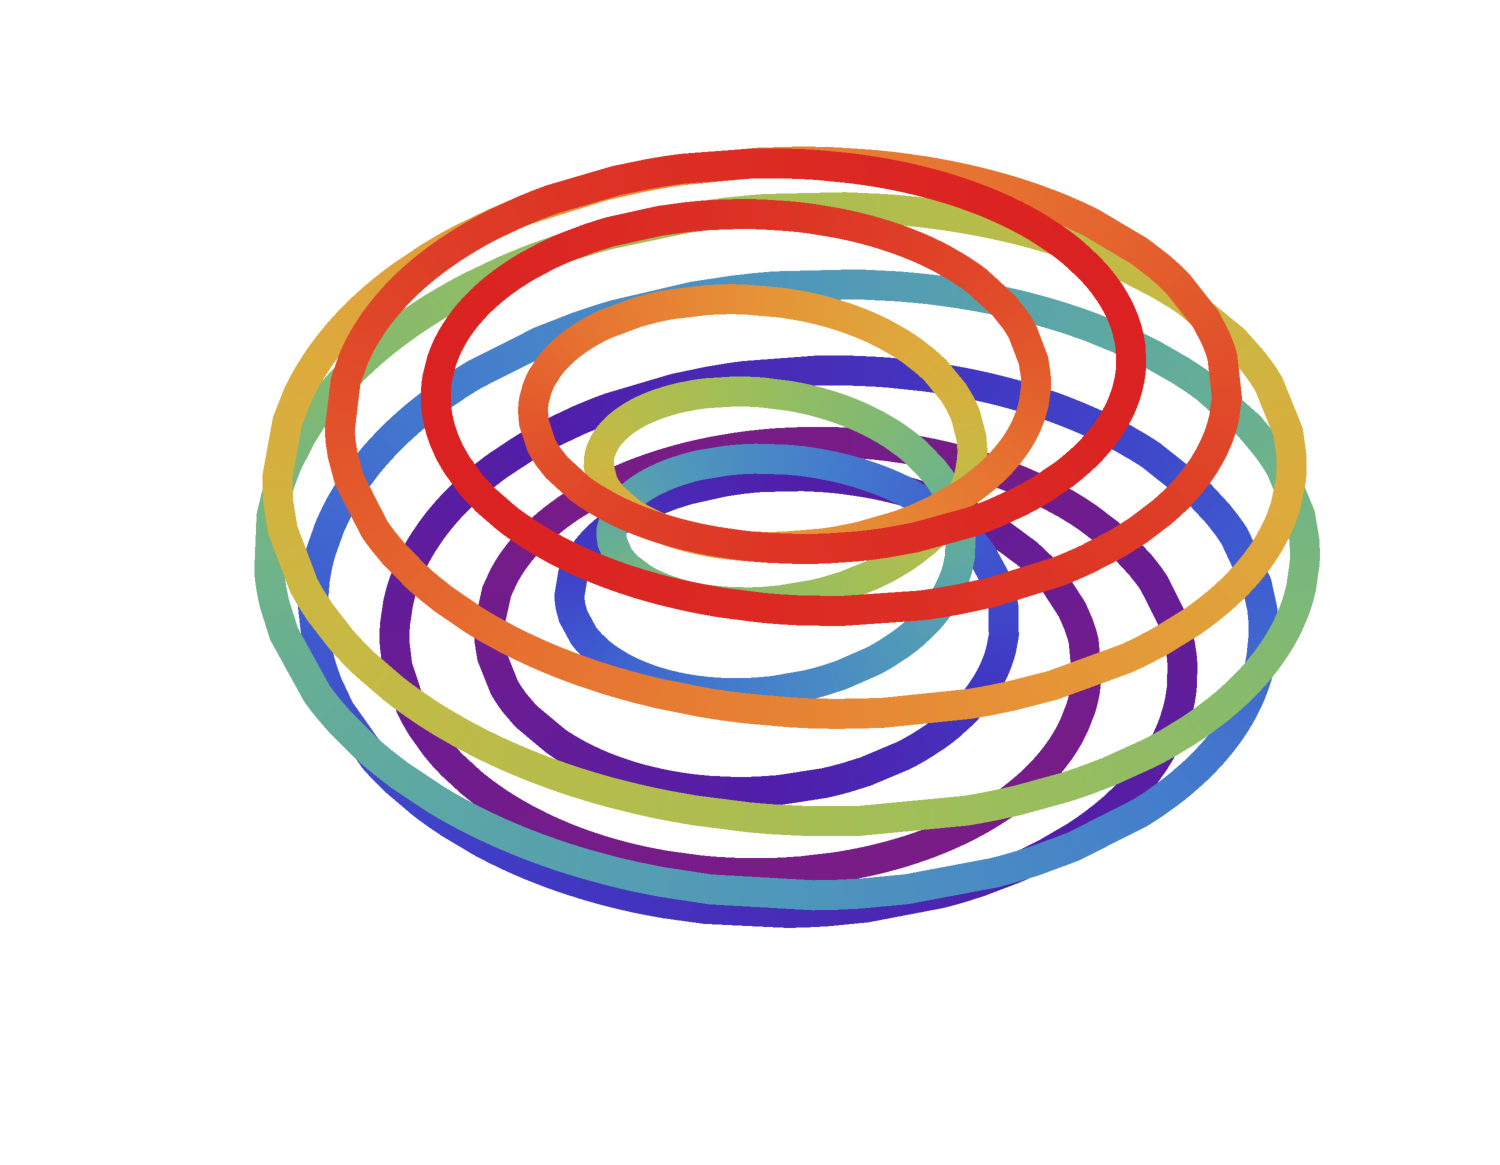
\includegraphics[width=\linewidth]{../data/torus-p11-q2.pdf}
        \subcaption{$p = 11, q = 2$}
    \end{minipage}
\end{figure}

Okazuje się, że innych obiektów już nie ma.

\begin{proposition}
    Jeśli żadna ze składowych splotu torusowego nie jest postaci $K_{0, 0}$ lub $K_{1, 0}$, to splot ten jest równoważny ze splotem $K_{q, r}$ dla pewnych $q, r$.
    Największy wspólny dzielnik indeksów $q, r$ jest jednocześnie liczbą składowych splotu.
\end{proposition}

%Węzeł ten leży na torusie $(r - 2)^2 + z^2 = 1$.
% p = 5;
% q = 3;
% ParametricPlot3D[
% {
% Cos [2 Pi p t] (2 + Cos[2 Pi q t]),
% (2 + Cos[2 Pi q t]) Sin[2 Pi p t],
% -Sin[2 Pi q t]},
% {t, 0, 1},
% ColorFunction -> "Rainbow",
% PlotStyle -> Thickness[0.02],
% Boxed -> False,
% Axes -> False
% ]

Nietrywialne węzły torusowe są pierwsze i odwracalne, ale nie achiralne (mają niezerową sygnaturę).

\begin{proposition}
    Dla $q, r > 0$ zdefiniujmy wielkość $\sigma(q, r) = - \sigma(K_{q, r})$.
    Wtedy, jeśli
    \begin{itemize}[leftmargin=*]
    \itemsep0em
        \item $2r < q$ i $r$ jest parzyste, to $\sigma(q, r) = \sigma(q-2r, r) + r^2$.
        \item $2r < q$ i $r$ jest nieparzyste, to $\sigma(q, r) = \sigma(q-2r, r) + r^2 - 1$.
        \item $\sigma(2r, r) = r^2 - 1$.
        \item jeśli $r \le q < 2r$ i $r$ jest parzyste, to $\sigma(q, r) + \sigma(2r-q, r) = r^2-1$.
        \item jeśli $r \le q < 2r$ i $r$ jest nieparzyste, to $\sigma(q, r) + \sigma(2r-q, r) = r^2-2$.
    \end{itemize}
    Co więcej, $\sigma(q, r) = \sigma(r, q)$, $\sigma(q, 1) = 0$, $\sigma(q, 2) = q-1$.
\end{proposition}

Dowód zawiera praca \cite{litherland81}.

\begin{proposition}
    Ustalmy względnie pierwsze $q, r$ takie, że $|q|, |r| \ge 2$.
    Splot $K(q, r)$ jest równoważny z odwrotnym do niego splotem $K(-q, -r)$.
\end{proposition}

Sploty $K(q, r)$ oraz $K(r, q)$ również są równoważne.
Murasugi prezentuje w książce \cite{murasugi96} przyjemny dowód opierający się na następującym lemacie:
Sfera $S^3$ powstaje z powierzchni dwóch węzłów trywialnych z wnętrzem ($D^2 \times S^1$) przez wzajemne sklejenie południka i równoleżnika z równoleżnikiem i południkiem.

% {\color{red} Longitude, meridian -- ustalić słownictwo}

Macierze Seiferta $M$ mają nieskomplikowaną blokową budowę, która może posłużyć do znalezienia wielomianu Alexandera (wzorem $\Delta = \det (M - tM^t)$).
Rachunki są nieco uciążliwe, oto ich wynik:

\begin{proposition}
    Wielomianem Alexandera splotu torusowego $K(q, r) \neq K(0,0)$ o $d$ składowych jest
    \[
        \Delta_{q, r}(t) = (-1)^{d-1} \frac{(1-t)(1 - t^{qr/d})^d}{(1-t^q)(1-t^r)} \left/t^{(q-1)(r-1)/2}\right. .
    \]
\end{proposition}

Znajomość wielomianu Alexandera wystarcza na szczęście do podania pełnej klasyfikacji węzłów torusowych bez uciążliwego dowodu.

\begin{proposition}
    Węzły torusowe $K(q, r)$, $K(p, s)$ są równoważne wtedy i tylko wtedy, gdy $\{q, r\} = \{p, s\}$ lub $\{q, r\} = \{-p, -s\}$.
\end{proposition}

\begin{proof}
    Ograniczymy się do przypadku, gdy $p, q, r, s \ge 2$.
    Tylko jedna implikacja wymaga dowodu, w prawo.
    Bez straty ogólności załóżmy więc, że $q > r$, $p > s$.
    Skoro węzły $K(q, r)$ i $K(p,s)$ są równoważne, to porównanie najwyższych współczynników w ich wielomianach Alexandera daje równość $(q-1)(r-1) = (p-1)(s-1)$.
    Wymnożenie wszystkiego prowadzi do czterech przypadków: $s = r$, $s = ps$, $qr = r$, $qr = ps$, z których dwa środkowe nie mogą zachodzić (gdyż $p, q > 1$).
    Z czwartego wynika, że $qr \le s < ps$, czyli sprzeczność.
\end{proof}

Podamy teraz wartości całkowitoliczbowych niezmienników dla węzłów torusowych przy założeniu, że $q$ lub $r$ nie jest zerem.

\begin{proposition}[Murasugi, 1991]
    Mamy $cr(K_{q,r}) = \min\{|q|(|r| -1), |r|(|q|-1)\}$.
\end{proposition}

Wyznaczenie indeksu rozwiązującego było dużo trudniejsze.
Murasugi pisze w książce \cite{murasugi96}, że mamy nierówność
\[
    u(K(q, r)) \le \frac 12 (q-1)(r-1),
\]
z równością dla względnie pierwszych $q, r > 0$.
Hipoteza Milnora głosiła, że w rzeczywistości równość zachodzi zawsze.
Dowód został odnaleziony w latach 1993-1995 przy użyciu tzw. \emph{gauge theory} (działu teorii pola, gdzie lagranżjan jest niezmienniczy względem grup Liego lokalnych transformacji...).
Patrz prace \cite{kronheimer93} oraz \cite{kronheimer95}.

\begin{proposition}[Kronheimer, Mrówka] \label{torus_unknotting}
    Dla względnie pierwszych $q, r > 0$ mamy
    \[
        u(K(q, r)) = \frac 12 (q-1)(r-1),
    \]
\end{proposition}

Genus pokrywa się z liczbą gordyjską dla węzłów (czyli względnie pierwszych $q, r$).

\begin{proposition} \label{torus_bridge}
    Indeksem mostowym węzła $K_{q,r}$ jest mniejsza z liczb $|q|, |r|$.
\end{proposition}

\begin{proposition}
    Mamy $\bracket{K_{2, n}} = A \bracket{K_{2,n-1}} + (-1)^{n-1} A^{2-3n}$
    oraz $\bracket{K_{2,1}} = -A^3$.
\end{proposition}

\begin{proposition}
    Wielomianem Jonesa węzła $(m, n)$-torusowego jest
    \[
        V(t) = \frac {t^{(m-1)(n-1):2}}{1-t^2} \cdot (1 - t^{m+1} - t^{n+1} + t^{m+n}).
    \]
\end{proposition}

Murasugi i Neuwirth w 1961 dla węzłów alternujących,
zaś Burde z Zieschangiem w 1965 pokazali, że nietrywialny węzeł,
którego grupa ma nietrywialne centrum, jest torusowy.

\begin{proposition}
    Wielomianem Alexandera węzła $(p,q)$-torusowego jest
    \[
         \Delta(T_{p,q}) = \frac{(t^{pq}-1)(t-1)}{(t^p-1)(t^q-1)}.
    \]
\end{proposition}

\begin{proof}
    Przypadek $p = 2$ wymaga prostego rozumowania indukcyjnego.
    Samo ćwiczenie pojawia się w wielu podręcznikach topologii.
    Pełny dowód można znaleźć w przykładzie 9.15 książki ,,Knots'' Burdego oraz Zieschanga.
    Inne podejście, tak zwaną formułę Seiferta-Torresa, prezentuje przeglądowa praca Turaewa ,,Reidemeister torsion in knot theory'', 119-182.
\end{proof}

\begin{corollary}
    Wielomian Alexandera odróżnia od siebie węzły $(2,n)$-torusowe.
\end{corollary}

\begin{proof}
    Mamy $\Delta(T_{2,n}) = (t^n+1) / (t+1)$, więc $\deg \Delta (T_{2,n}) = n - 1$.
\end{proof}

% Koniec sekcji Węzły torusowe


\section{Węzły satelitarne}

% DIKTJONARY;latitude;szerokość geograficzna;geografia
% DIKTJONARY;longitude;długość geograficzna;geografia
% DIKTJONARY;meridian (of longitude);południk;geografia
% DIKTJONARY;parallel (of latitude);równoleżnik;geografia
% DIKTJONARY;---;geografia;-
% to jest powtórzenie np. z pliku 103a
Załóżmy, że w dopełnieniu pewnego splotu został zanurzony torus.
Jeżeli jest ściśliwy, to albo równoleżnikl torusa ogranicza dysk w dopełnieniu splotu~i torus jest niezawęźlony, albo południk ogranicza dysk w dopełnieniu splotu i~splot nie przebiega wzdłuż torusa.
Żadna z~tych sytuacji nie jest ciekawa.
Inny zdegenerowany przypadek występuje, gdy torus stanowi rurowe otoczenie jednego z~ogniw splotu.
W przeciwnym razie splot można zbudować z~prostszych obiektów.

Oto formalny opis konstrukcji.
Niech $W$ będzie pełnym torusem.
Dysk zanurzony w $W$, którego brzeg stanowi nieściągalną pętlę w $\partial W$, nazywamy południkowym.
Mówimy, że zamknięta krzywa $\lambda \subseteq W$ jest właściwa, jeżeli przecina wszystkie dyski południkowe.

\begin{definition}[węzeł satelitarny]
    \index{węzeł!satelitarny}
    Niech $P$ będzie splotem zanurzonym w~niezawęźlonym torusie $W$ tak, by co najmniej jedno z~ogniw stanowiło właściwą pętlę w~$W$.
    Niech $C$ będzie węzłem, zaś $V$ jego rurowym otoczeniem.
    Wybierzmy dowolny homeomorfizm $h \colon W \to V$.
    Wtedy splot $S = h(P)$ nazywamy satelitą o~wzorcu $P$ oraz towarzyszu $C$.
\end{definition}

% \begin{definition}
%     Węzeł nazywamy satelitarnym, jeśli zawiera nieściśliwy, nierównoległy do brzegu torus we własnym dopełnieniu.
% \end{definition}

Hoste i inni podejrzewają w~\cite{thistlethwaite98}, że jeśli satelita owija się $m$-krotnie wokół torusa, zaś indeks skrzyżowaniowy towarzysza wynosi $k$, to satelita nie posiada diagramu o~mniej niż $km^2$ skrzyżowaniach.
\index[persons]{Hoste, Jim}%
\index[persons]{Thistlethwaite, Morwen}%
\index[persons]{Weeks, Jeff}%

Ponieważ dla trójlistnika $k = 3$, napotkali się tylko na satelity owijające się $m = 2$ razy podczas tablicowania pierwszych węzłów do 16 skrzyżowań.
Nie spodziewano się żadnego satelity ósemki, gdyż wtedy $k = 4$, zatem każdy satelita miałby co najmniej $4 \cdot 2^2 + 1 = 17$ skrzyżowań: dodatkowe $+1$ jest potrzebne, by nie dostać splotu o~dwóch ogniwach.

Najprostszy satelita ma 13 skrzyżowań.
Ze strony internetowej programu Regina można dowiedzieć się dokładniej, jak wygląda rozkład satelitów wśród małych węzłów:

\renewcommand*{\arraystretch}{1.4}
\footnotesize
\begin{longtable}{lccccccc}
    \hline
    \textbf{skrzyżowania} & 13 & 14 & 15 & 16 & 17 & 18 & 19 \\ \hline \endhead
    węzły pierwsze, satelitarne & 2 & 2 & 6 & 10 & 29 & 86 & 245 \\
    \hline
\end{longtable}
\normalsize

Razem 380 węzłów.

\begin{example}[torus połykająco-podążający]
\label{swallow_follow_torus}
% DICTIONARY;swallow-follow;połykająco-podążający;torus
% DICTIONARY;torus;torus;-
    Klasa węzłów satelitarnych obejmuje węzły złożone.
    W ich przypadku można wskazać pewien szczególny torus nieściśliwy -- połykający pierwszy składnik, a~potem podążający za drugim:\footnote{Źródło obrazka: \url{https://mcm-www.jwu.ac.jp/~hayashic/semi/07/07i/07i.html}}
    \begin{figure}[H]
        \centering
        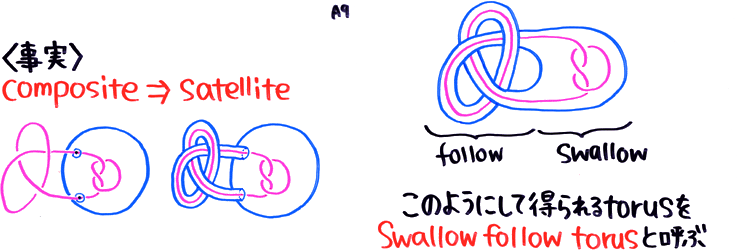
\includegraphics[width=0.75\linewidth]{../data/mixed/follow-swallow.png}
        \caption[something]{Torus połykająco-podążający. Źródło: strona internetowa  C. Hayashiego.}
    \end{figure}
\end{example}

Schubert pokazał, że zorientowane klasy izotopii węzłów w~$S^3$ tworzą wolny przemienny monoid na przeliczalnie wielu generatorach.
\index[persons]{Schubert, Horst}%
Dowód to uważna analiza nieściśliwych torusów obecnych w~dopełnieniu sumy spójnej.
To doprowadziło go do definicji węzłów satelitarnych i~towarzyszących w~przełomowej pracy \cite{schubert53} oraz zunifikowało teorię 3-rozmaitości z teorią węzłów.
Może warto zapoznać się z pracą Motegiego \cite{motegi97}?
Wikipedia mówi, że zapis węzła jako satelity nie jest jednoznaczny, a~tam mogą być przykłady.
%=% https://en.wikipedia.org/wiki/Satellite_knot#cite_ref-7

Na brzegu torusa $V$ można wprowadzić pewien układ współrzędnych: południk to pętla właściwa w $\partial V$, która ogranicza dysk w $V$, natomiast równoleżnik to pętla w $\partial V$, która spotyka południk raz.
Z~dokładnością do izotopii południk jest jeden, ale równoleżnik nie.
Równoleżnik preferowany to taki, którego indeks zaczepienia z~rdzeniem torusa wynosi zero.

\begin{definition}[dubel Whiteheada]
\index{dubel Whiteheada}%
    Jeżeli $P \subseteq W$ jest skręconym jednokrotnie niewęzłem, to węzeł $S$ nazywamy dublem Whiteheada.
\end{definition}

Każdy węzeł posiada nieskończenie wiele dubli Whiteheada: wystarczy rozciąć torus $V$, skręcić jedną końcówkę i~ponownie zszyć, żaden z~nich nie jest odróżniany od niewęzła przez wielomian Alexandera.

Wyróżnia się pewien szczególny homeomorfizm $h$, który przenosi południk i preferowany równoleżnik $W$ na południk i preferowany równoleżnik $V$.
Nazywamy go wiernym.
% DICTIONARY;faithful homeomorphism;homomorfizm wierny;-
O dublu względem wiernego homeomorfizmu mówimy, że jest nieskręcony.
% TODO: skąd powyższe zdanie? jak jest nieskręcony po angielsku?
% Kawauchi około strony 32? (Ten z 1996)

\begin{definition}[węzeł kablowy]
\index{węzeł!kablowy}%
    Niech $h \colon W \to V$ będzie wiernym homeomorfizmem, zaś $P$ węzłem $(p, q)$-torusowym.
    Satelitę $S$ nazywamy węzłem $(p, q)$-kablowym albo krótko kablem.
\end{definition}

\begin{proposition}
    Każdy kabel wyznacza jednoznacznie węzeł, z~którego powstał.
\end{proposition}

\begin{proof}
\index[persons]{Feustel, Charles}%
\index[persons]{Whitten, Wilbur}%
    Wniosek 2 z~pracy \cite{feustel78} Feustela, Whittena pokazuje, że na podstawie kabla można wyznaczyć parametry węzła torusowego $K'_{p,q}$ oraz topologię dopełnienia oryginalnego węzła.
    Wiemy jednak z~twierdzenia Gordona-Lueckego, że różne węzły PIERWSZE mają różne dopełnienia.
\end{proof}

Niewęzeł nie ma nietrywialnych węzłów towarzyszących.

\begin{definition}
    Towarzysza $C$ nietrywialnego splotu nazywamy właściwym, jeśli nie jest niewęzłem i~nie jest ogniwem tego splotu.
\end{definition}

Sploty bez właściwych towarzyszy określa się zazwyczaj terminem ,,atoroidalny''.
\index{splot!atoroidalny}%
Patrz też diagram przedstawiony w \cite{cromwell04} na stronie 83.

Schubert \cite{schubert54} zastanawiał się, czy węzeł może mieć nieskończenie wiele towarzyszy.
Udzielił negatywnej odpowiedzi: satelita $S$ z towarzyszem $C$ oraz wzorcem indeksu $k$ spełnia nierówność $\bridge(S) \ge k \cdot \bridge(C)$; z drugiej strony tylko niewęzeł jest 1-mostowy.
(Patrz też wstęp do \cite{schultens03}).
% wiem to z pracy schultens03

\begin{proposition}
    Duble nietrywialnych węzłów oraz kable są pierwsze.
\end{proposition}

\begin{proof}
    Prosty wniosek z~twierdzenia 4.4.1 w~\cite[s. 84]{cromwell04}: jeżeli wzorzec jest niewęzłem lub węzłem pierwszym, to każdy właściwy satelita jest pierwszy.
\end{proof}

Niektóre węzły przedstawiają się jako satelity w~dokładnie jeden sposób, inne nie.
Rok 1979 przyniósł amerykańską pracę \cite{jaco79} oraz niemiecką książkę\footnote{Według recenzji Hempela, najważniejsze tam jest twierdzenie klasyfikacyjne: niech $M_1, M_2$ będą 3-rozmaitościami Hakena \index{rozmaitość!Hakena} z brzegiem, zaś $V_1, V_2$ ich podrozmaitościami charakterystycznymi, wtedy każda homotopijna równoważność $f \colon M_1 \to M_2$ można zdeformować tak, że jest homeomorfizmem między domknięciami: $M_1 \setminus V_1$ oraz $M_2 \setminus V_2$ i~homotopijną równoważnością między $V_1$ oraz $V_2$.} \cite{johannson79}, gdzie niezależnie od siebie opisano jednoznaczny rozkład (nazywany teraz) Jaco-Shalena-Johannsona:
\index{rozkład Jaco-Shalena-Johannsona}%
\index[persons]{Jaco, William}%
\index[persons]{Shalen, Peter}%
\index[persons]{Johannson, Klaus}%

\begin{proposition}
    Niech $M$ będzie nierozkładalną, orientowalną, domkniętą 3-rozmaitością.
    Istnieje wtedy jedyna z dokładnością do izotopii minimalna rodzina rozłącznie zanurzonych nieściśliwych torusów tak, że każda składowa 3-rozmaitości powstałej przez rozcinanie wzdłuż torusów jest atoroidalna lub włóknistą przestrzenią Seiferta ($S^1$-wiązką nad dwuwymiarowym orbifoldem).
\index{orbifold}%
\index{rozmaitość!atoroidalna}%
\index{przestrzeń!włóknista Seiferta}%
\index{wiązka ($S^1$)}%
\end{proposition}

Jest on związany z operacją złączania (ang. \emph{splicing}), będącej uogólnieniem budowania satelitów, sumy spójnej, dubli Whiteheada i kasowania ogniwa.
\index{złączanie (splicing)}%
% https://arxiv.org/pdf/math/0506523.pdf
% DICTIONARY;splicing;złączanie;-
Hipotezę o jedyności rozkładu wysnuł wcześniej Waldhausen.
\index[persons]{Waldhausen, Friedhelm}%

% Koniec sekcji Węzły satelitarne


\section{Węzły hiperboliczne} % (fold)
\label{sec:hyperbolic}
Jak pisaliśmy w sekcji \ref{mutants_mutation}, słynne węzły Conwaya oraz Kinoshity-Terasakiego odróżnił od siebie po raz pierwszy przez Rileya.
Zbadał paraboliczne reprezentacje ich grup w skończoną grupę prostą $PSL(2, 7)$, co doprowadziło go do odkrycia w dopełnieniu ósemki struktury hiperbolicznej \cite{riley75}.
% https://arxiv.org/pdf/2002.00564.pdf
Zainspirowany tym wynikiem Thurston najpierw rozłożył dopełnienie ósemki na dwa idealne wielościany, a potem znacznie uogólnił swój przykład.

Reszta sekcji powstała na podstawie przeglądowej pracy \cite{purcell19} Futera, Kalfagianniego, Purcell i innych oraz notatek z~wykładów, które były prowadzone przez samą Purcell.
Wiedzę o~węzłach hiperbolicznych można czerpać także z~artykułu: \cite{weeks05} Weeksa.
Poprawiona wersja dostępna w~serwisie arXiv.

% Badając sploty nie ograniczamy się tylko do diagramów, ale korzystamy też z ich dopełnień, to znaczy 3-rozmaitości $S^3 \setminus L$.
% Jest ona homeomorficzna z wnętrzem zwartej rozmaitości $X(L) = S^3 \setminus N(K)$, zwanej zewnętrzem splotu, gdzie $N(L)$ stanowi rurowe otoczenie splotu.
% Dalej możemy stosować maszynierę topologii 3-rozmaitości.

% \begin{definition}[ściśliwy]
%     Niech orientowalna powierzchnia $S$ będzie właściwie\footnote{properly} zanurzona w zwartej, orientowalnej 3-rozmaitości $M$.
%     Załóżmy, że dla każdego dysku $E \subseteq M$ z brzegiem $\partial E \subseteq S$ istnieje dysk $E' \subseteq S$ taki, że $\partial E = \partial E'$.
%     Mówimy wtedy, że powierzchnia $S$ jest nieściśliwa.
% \end{definition}

% $\partial$-ściśliwość

% essential

% Haken

% monodromy of fibration

% Węzły i sploty, które będziemy rozpatrywać dalej, mają szczególną strukturą geometryczną.

\begin{definition}[hiperboliczny]
    \index{węzeł!hiperboliczny}
    Splot $L$, na dopełnieniu którego można zadać zupełną metrykę o stałej krzywiźnie $-1$ nazywamy hiperbolicznym.
\end{definition}

\begin{proposition}
    Splot $L$ jest hiperboliczny wtedy i tylko wtedy, gdy $S^3 \setminus L = \mathbb H^3 / \Gamma$, gdzie $\mathbb H^3$ to hiperboliczna 3-przestrzeń, zaś $\Gamma$ jest dyskretną, beztorsyjną grupą izometrii, izomorficzną z $\pi_1(S^3 \setminus L)$.
\end{proposition}

Thurston podejrzewał, że każda 3-rozmaitość rozkłada się wzdłuż sfer i nieściśliwych torusów na części wyposażone w jedną z ośmiu kanonicznych geometrii:
\begin{itemize}
\item sferyczną $S^3$,
\item euklidesową $E^3$,
\item hiperboliczną $H^3$,
\item $S^2 \times \R$,
\item $H^2 \times \R$,
\item uniwersalne nakrycie $SL(2, \R)$,
\item geometrię Sol albo
\item geometrię Nil.
\end{itemize}
Nie umiał podać pełnego uzasadnienia, w 1982 roku udowodnił swoje przypuszczenie dla rozmaitości Hakena.
Dowód hipotezy geometryzacyjnej dostarczył mniej więcej dwie dekady później Perelman, nie to jest jednak dla nas najważniejsze.

Thurston pokazał też, że dopełnienie węzła jest rozmaitością włóknistą Seiferta, toroidalną albo hiperboliczną.
Innymi słowy, przedstawił trychotomię:
\begin{theorem}
    \index{twierdzenie!Thurstona}
    Każdy węzeł jest satelitarny, torusowy albo hiperboliczny.
\end{theorem}

Węzły hiperboliczne stanowią najliczniejszą i najmniej zrozumianą rodzinę węzłów.

\begin{proof}
    Thurston w \cite{thurston82}.
\end{proof}

Dwa lata później Menasco \cite{menasco84} pokazał, że każdy pierwszy, alternujący splot jest albo 2-warkoczem (a zatem, torusowy) albo hiperboliczny.

\begin{corollary}
    Każdy węzeł hiperboliczny jest pierwszy.
\end{corollary}

Prawie każdy węzeł pierwszy o~mniej niż 17 skrzyżowaniach jest hiperboliczny, na 32 wyjątki składa się 12 węzłów torusowych oraz 20 satelitów trójlistnika.
Te ostatnie mają co najmniej 11 skrzyżowań.
Baza ciągów liczb całkowitych OEIS zawiera informacje na temat liczności poszczególnych typów węzłów.
Analizując ciągi A051764, A051765 oraz A052408 można dojść do wniosku, że wraz ze wzrostem liczby skrzyżowań, stosunek liczby węzłów hiperbolicznych do wszystkich węzłów dąży do $1$:

\begin{figure}[H]
\renewcommand*{\arraystretch}{1.4}
\footnotesize
\begin{longtable}{lcccccccccccccc}
\hline
    \textbf{rodzaj} & 3 & 4 & 5 & 6 & 7 & 8  & 9  & 10  & 11  & 12   & 13   & 14    & 15     \\ \hline \endhead
    torusowe        & 1 & 0 & 1 & 0 & 1 & 1  & 1  & 1   & 1   & 0    & 1    & 1     & 2      \\
    satelitarne     & 0 & 0 & 0 & 0 & 0 & 0  & 0  & 0   & 0   & 0    & 2    & 2     & 6      \\
    hiperboliczne   & 0 & 1 & 1 & 3 & 6 & 20 & 48 & 164 & 551 & 2176 & 9985 & 46969 & 253285 \\
    \hline
\end{longtable}
\normalsize
\end{figure}

W pracy \cite{malyutin16} A. Malyutin pokazał jednak, że to przypuszczenie jest sprzeczne z~wieloma innymi starymi hipotezami teorii węzłów: \ref{malyutin1} -- \ref{malyutin4}.

\begin{conjecture}
    \label{malyutin1}
    Indeks skrzyżowaniowy jest addytywny względem sumy spójnej.
\end{conjecture}

(To jest powtórzenie hipotezy \ref{cnj:crossing_additive}).
Murasugi dowiódł prawdziwości hipotezy dla węzłów alternujących, w~pracy \cite{murasugi87} jest to wniosek z~dowodu hipotezy Taita.
Krótko po tym Lickorish, Thistlethwaite powtórzyli to dla węzłów adekwatnych w \cite{lickorish88}.
Na początku XX wieku Diao \cite{diao04} oraz Gruber \cite{gruber03} niezależnie udowodnili hipotezę \ref{malyutin1} dla pewnej szerokiej klasy węzłów, obejmującej wszystkie węzły torusowe oraz wiele węzłów alternujących oraz pewne inne obiekty, których nie chcemy opisywać.

\begin{conjecture}
    Satelita ma większy (w słabszej wersji: nie mniejszy) indeks skrzyżowaniowy niż jego towarzysze.
\end{conjecture}

Lackenby pokazał w~\cite{lackenby14}, że jeśli $K$ jest satelitą z towarzyszem $L$, to $\operatorname{cr} K \ge 10^{-13} \operatorname{cr} L$.

\begin{conjecture}
    Węzeł złożony ma większy (w słabszej wersji: nie mniejszy) indeks skrzyżowaniowy niż jego faktory.
\end{conjecture}

Mówimy, że węzeł pierwszy $P$ jest $\lambda$-regularny, jeśli $cr K \ge \lambda \cdot cr P$ za każdym razem, gdy węzeł $P$ jest faktorem węzła $K$.
Zatem hipotezę można wysłowić krótko ,,węzły pierwsze są $1$-regularne''.
Na podstawie prac Murasugiego, Kauffmana i~Thistlethwaite'a z~końca lat 80. wiemy, że zachodzi dla węzłów alternujących.
Diao pokazał w \cite[tw. 3.8]{diao04}, że węzły torusowe także są $1$-regularne, natomiast Lackenby przedstawił w~\cite{lackenby09} rozumowanie, dlaczego wszystkie węzły są $1/152$-regularne.
Pisaliśmy o tym w podsekcji \ref{sub:crossing_number}.

\begin{conjecture}
    \label{malyutin4}
    Węzły pierwsze są $2/3$-regularne.
\end{conjecture}

Rozwiązanie zagadki przyniosła praca samego Malyutina \cite{malyutin19} opublikowana latem 2019 roku, przynajmniej dla splotów.
Pokazał w~niej, że jeśli oznaczymy liczbę splotów pierwszych i~nierozszczepialnych o~$n$ lub mniej skrzyżowaniach przez $P_n$, zaś liczbę hiperbolicznych splotów, także o~$n$ lub mniej skrzyżowaniach, przez $H_n$, prawdziwe będzie oszacowanie
\begin{equation}
    \liminf_{n \to \infty} \frac{H_n}{P_n} < 1 - 10^{-13}.
\end{equation}

% Every non-split, prime, alternating link that is not a~torus link is hyperbolic by a~result of William Menasco.

% https://arxiv.org/abs/math/0309466
% https://arxiv.org/abs/math/0311380

Czwarty rozdział książki \cite{purcell2020} zawiera ćwiczenie, by znaleźć dwuparametrową rodzinę zupełnych struktur hiperbolicznych na dziurawym torusie oraz czterokrotnie dziurawej sferze.
Elastyczność tego rodzaju nie występuje w przestrzeniach wyższych wymiarów.
Z twierdzenia o sztywności, w wersji algebraicznej:

\begin{theorem}[Mostow-Prasad]
    \index{twierdzenie!o sztywności}
    Niech $\Gamma_1, \Gamma_2$ będą dyskretnymi podgrupami grupy izometrii $\mathbb H^n$ dla $n \ge 3$ takimi, że ilorazy $\mathbb H^n$ mają skończone objętości.
    Załóżmy też, że istnieje izomorfizm grup $\varphi \colon \Gamma_1 \to \Gamma_2$.
    Wtedy podgrupy $\Gamma_1, \Gamma_2$ są sprzężone.
\end{theorem}

albo geometrycznej:

\begin{theorem}[Mostow-Prasad]
    Niech $M_1, M_2$ będą zupełnymi, hiperbolicznymi rozmaitościami o skończonych objętościach.
    Wtedy każdy izomorfizm grup podstawowych $\varphi \colon \pi_1(M_1) \to \pi_1(M_2)$ realizowany jest jednoznacznie przez izometrię.
\end{theorem}

wynika, że jeśli znaleźliśmy jakąś zupełną strukturę hiperboliczną na dopełnieniu splotu, to innych już nie ma. 
Dzięki temu niezmienniki mające korzenie w geometrii hiperbolicznej mają przyjemne własności.
Patrz także oryginalne prace: Mostowa \cite{mostow73}, Prasada \cite{prasad73}.

\begin{proof}
    Thurston przedstawił szkic rozumowania w sekcji 5.9 swoich notatek, na bazie których powstała później książka \cite{thurston97}.
    Inne szczegółowe rozumowanie można znaleźć w rozdziale C podręcznika \cite{benedetti92}.
\end{proof}

% luźno związane: http://www.deltami.edu.pl/temat/matematyka/topologia/2012/12/27/%William_Thurston_i_hipoteza_geometryzacyjna/

\begin{tobedone}[kryterium Thurstona]
    Niech $L$ będzie splotem z dopełnieniem $X$ i grupą podstawową $\pi = \pi_1(X)$.
    Jeżeli spełnione są następujące warunki:
    \begin{enumerate}
    \item $L$ nie rozszczepia się,
    \item $L$ nie jest niewęzłem,
    \item żadna składowa $L$ nie jest niezakłóconym węzłem satelitarnym (?),
    \item $L$ nie jest węzłem torusowym,
    \end{enumerate}
    to $L$ jest splotem hiperbolicznym.
    Warunki podane wyżej mają swoje odpowiedniki dla przestrzeni $X$ ($X$ nie zawiera właściwej 2-sfery, właściwego dysku, właściwego torusa, właściwego pierścienia) oraz grupy $\pi$ ($\pi$ nie jest wolnym produktem, nie jest cykliczna oraz nie zawiera kopii $\Z^2$).
\end{tobedone}

\begin{proposition}
    Grupa symetrii węzła hiperbolicznego jest skończona: cykliczna lub diedralna.
\end{proposition}

Uwaga -- nie chodzi tutaj ani o grupę węzła, ani grupę kolorującą, ale prawdopodobnie grupę automorfizmów zewnętrznych grupy $\pi_1(S^3 \setminus K)$.

\begin{proof}
    Pierwszy był Riley w artykule \cite{riley75}, można też zapoznać się z późniejszą pracą \cite{kodama92} Kodamy.
\end{proof}

% objętość

Twierdzenie Mostowa-Prasada pozwala nam na wprowadzenie nowych niezmienników splotów hiperbolicznych: wystarczy wziąć dowolny geometryczny niezmiennik dopełnienia węzła.
Najważniejszym z nich wydaje się być objętość.

\begin{definition}[objętość]
    Niech $L$ będzie splotem hiperbolicznym.
    Objętość dopełnienia $L$ względem zupełnej metryki hiperbolicznej nazywamy objętością splotu $L$ i oznaczamy $\volume L$.
\end{definition}

Objętość jest zawsze skończoną liczbą rzeczywistą.
Dla wygody przyjmuje się czasami, że objętość węzłów torusowych oraz satelitarnych wynosi $0$.
Komputerowy program SnapPea napisany przez J. Weeksa pozwala na wyznaczenie objętości dowolnego splotu o rozsądnej ilości skrzyżowań.

\begin{example}
    $\volume 4_1 \approx 2.0298832$.
\end{example}

Patrz też ciąg A091518 w bazie danych OEIS.

\begin{proposition}
    \label{least_volume}
    Żaden węzeł nie ma mniejszej objętości hiperbolicznej od ósemki.
\end{proposition}

\begin{proof}
    Cao, Meyerhoff w \cite{cao01} przeanalizowali pakowania horokul w uniwersalnym nakryciu związanym z rozmaitościami.
    Doszli do wniosku, że nie ma tam dostatecznieo wolnego miejsca, jeżeli ostrze (cusp) nie jest odpowiedniego rozmiaru.
    Trzykrotnie wspierają się przy tym pomocą komputera, by sprawdzić, że określone warunki są spełnione we wszystkich punktach danej przestrzeni parametrów.
\end{proof}

\begin{example}
    $\volume 5_2 \approx 2.82812$.
\end{example}

W encyklopedii Wolfram Mathworld znajduje się informacja, że $5_2$ oraz pewien węzeł o~dwunastu skrzyżowaniach mają tę samą objętość, prawdopodobnie chodzi tu o~$12n_{242}$, który znany jest także jako $(-2, 3, 7)$-precel. 

\begin{example}
    $\volume 6_1 \approx 3.16396$.
\end{example}

\begin{example}
    $\volume 6_2 \approx 4.40083$.
\end{example}

\begin{example}
    $\volume 6_3 \approx 5.69302$.
\end{example}

\begin{example}
    $\volume 7_4 \approx 5.13794$.
\end{example}

\begin{example}
    Niech $K$ będzie jednym z dwóch węzłów w parze Perko.
    Wtedy $\volume K \approx 5.63877$.
\end{example}

Praca \cite{purcell19} wspomina kilka przyjemnych ograniczeń, jakie musi spełniać objętość.
Aby je przytoczyć, musimy najpierw zdefiniować dwie stałe: $v_4$ oraz $v_8$, objętość idealnego czworościanu (odpowiednio: ośmiościanu) foremnego w $\mathbb H^3$.
Mamy
\begin{align}
    v_4 & = 1.0149\ldots \\
    v_8 & = 3.6638\ldots
\end{align}

I tak najpierw Adams pokazał:

\begin{proposition}
    Niech $D$ będzie diagramem hiperbolicznego splotu o $\operatorname{cr} L \ge 5$ skrzyżowaniach.
    Wtedy
    \begin{equation}
        \volume (S^3 \setminus K) \le 4 (\operatorname{cr} D - 4) v_4.
    \end{equation} 
\end{proposition}

A później poprawił wswój wynik:

\begin{proposition}
    Niech $D$ będzie diagramem hiperbolicznego splotu o $\operatorname{cr} L \ge 5$ skrzyżowaniach.
    Wtedy
    \begin{equation}
        \volume (S^3 \setminus K) \le 4 (\operatorname{cr} D - 5) v_8 + 4v_4.
    \end{equation} 
\end{proposition}

Jego metoda polega na podzieleniu dopełnienia splotu na czterościany i ośmiościany oraz policzeniu ich.
To, w połączeniu ze znanymi ograniczeniam na objętość ,,cegiełek'', wystarcza.
Podział na ośmiościany zaproponował Dylan Thurston (nie mylić z Williamem!).

% Wiki

Thurston zauważył, że tylko skończenie wiele hiperbolicznych 3-rozmaitości może mieć tę samą objętość -- wynika to z prac Gromova i Jørgensena.
Następnie Wielenberg przedstawił w~\cite{wielenberg81} przykłady pokazujące, że istnieją dowolnie duże kolizje wśród węzłów hiperbolicznych: pewne podgrupy klasycznej grupy Picarda działają  na półprzestrzeni hiperbolicznej wymiaru 3 i mają przy tym fundamentalne wielościany identyczne jako zbiory, ale znacząco różne w~sposobie, w jaki zidentyfikowano ich ściany.

Na przykład mutacja węzła hiperbolicznego nigdy nie zmienia objętości \cite{ruberman87}, \cite[s. 124]{adams94}.
Praktyka pokazuje jednak, że niezmiennik dobrze wspomaga proces tablicowania węzłów.

\begin{proposition}
    Objętości hiperboliczne 3-rozmaitości tworzą dobrze uporządkowany podzbiór $\R$, typu $\omega^\omega$.
\end{proposition}

\begin{proof}
    Wikipedia twierdzi, że dowód jest gdzieś w \cite{neumann85}, ja tego nie widzę.
\end{proof}

W dowolnej rodzinie węzłów istnieje element o najmniejszej objętości.
Dla orientowalnych, niezwartych hiperbolicznych 3-rozmaitości, klasy obejmującej dopełnienia hiperbolicznych węzłów, najmniejszą objętość posiada dopełnienie ósemki oraz jej bliźniak, otrzymany przez $(5, 1)$-chirurgię jednego z ogniw splotu Whiteheada.
To jest fakt \ref{least_volume}.
Natomiast wśród orientowalnych 3-rozmaitości o dwóch ostrzach najmniejszą objętość, ma $(-2, 3, 8)$-precel oraz splot Whiteheada: Agol pokazał to w \cite{agol10}.
Ich objętość wynosi
\begin{equation}
    v_8 = 4 \sum_{n=0}^\infty \frac{(-1)^n}{(2n+1)^2} = \approx 3.6638623767. % ... 08876060218414059729536443096597497126688537065 ...
\end{equation}
Yoshida \cite{yoshida13} znalazł splot z najmniejszą objętością równą $2v_8$ wśród tych o 4 ogniwach, sploty o 3 ogniwach nie są zbyt dobrze zrozumiane.

% Koniec sekcji Węzły hiperboliczne

\section{Węzły plastrowe} % (fold)
\label{sec:slice}
% Na podstawie podręcznika Murasugiego
Rozpatrzmy węzeł $K$ w~sferze $S^3$ jako brzegu czterowymiarowej kuli $B^4$.
Punkt wewnętrzny $P$ dysku $D$ w~tej kuli nazywamy osobliwym, jeśli nie można wskazać dla niego żadnego otoczenia $U$, homeomorficznego z~$B^4$, takiego że $\partial U \cap D$ jest węzłem trywialnym w~$\partial U$, 3-sferze.
Jeśli $K$ jest brzegiem dysku $D$ pozbawionego punktów osobliwych, to jest on węzłem plastrowym.

W tej sekcji opiszemy pewną czterowymiarową własność węzłów.
Węzły plastrowe na sferze $S^3$ to takie, które są brzegiem ładnie zanurzonego dysku $D$ w~4-kuli.
Co dokładnie znaczy wyrażenie ,,ładnie zanurzony'' zależy od kontekstu: istnieją węzły gładko albo też topologicznie plastrowe.
Precyzuje to pochodząca najwyraźniej od Foxa (1962) definicja:

\begin{definition}
    \index{węzeł!plastrowy}
    Węzeł $K \subseteq S^3$ nazywamy plastrowym, jeśli istnieje płaski dysk $D$ zawarty w~$B^4$ taki, że $K = \partial D = D \cap S^3$.
    Płaski, czyli: dysk $D$ posiada otoczenie $N$ będące kopią zbioru $D \times I^2$, która spotyka sferę $S^3$ dokładnie w~$\partial D \times I^2$.
\end{definition}

Następujące węzły o~mniej niż jedenastu skrzyżowaniach są plastrowe: $6_1$, $8_{20}$, $8_{8}$, $8_{9}$, $9_{27}$, $9_{41}$, $9_{46}$, $10_{22}$, $10_{35}$, $10_{3}$, $10_{42}$, $10_{48}$, $10_{75}$, $10_{87}$, $10_{99}$, $10_{123}$, $10_{129}$, $10_{137}$, $10_{140}$, $10_{153}$, $10_{155}$, $10_{155}$.
Lista ta powstała na podstawie portalu KnotAtlas.

\begin{proposition} \label{slice_square_det}
    Wyznacznik węzła plastrowego jest kwadratem (Rolfsen 1976, strona 224).
\end{proposition}

Węzły plastrowe (slice), skręcone (twist).

\begin{definition} \label{twist_knots}
    \index{węzeł!skręcony}
    Węzeł powstały przez $n$-krotne półskręcanie domkniętej pętli oraz splecienie końców nazywamy węzłem skręconym.
\end{definition}

Węzły skręcone to dokładnie towarzyszące niewęzłowi w~węzłach satelitarnych, tak zwane whiteheadowskie duble niewęzła.
Wszystkie są odwracalne (ale tylko niewęzeł oraz ósemka są amfichiralne) i~mają liczbę gordyjską $1$, ponieważ wystarczy rozwiązać skrzyżowanie, które plotło końce.
Każdy jest $2$-mostowy i~posiada zerową sygnaturę.
Dalsze własności węzłów skręconych zależą od $n$, ilości półskrętów.
Indeks skrzyżowaniowy wynosi $n + 2$.

\begin{proposition}
    Wielomianowymi niezmiennikami węzłów skręconych są:
    \begin{align*}
    (q+1)\jones(q) & = \begin{cases}
        1+q^{-2}+q^{-n}-q^{-n-3} & n \mbox{ nieparzyste} \\
        q^{3}+q-q^{3-n}+q^{-n} & n \mbox{ parzyste}
    \end{cases} \\
    2 \conway (z) & = \begin{cases}
        (n+1) z^{2} + 2 & n \mbox{ nieparzyste} \\
        2 - nz^2 & n \mbox{ parzyste}
    \end{cases}
    \end{align*}
\end{proposition}

%\begin{definition}
    %Węzeł $K$ w~$S^3 = \partial D^4$ jest plastrowy, jeśli ogranicza dysk $\alexander^2$ w~$D^4$, który ma rurowe otoczenie $\alexander^2 \times D^2$, którego przekrojem z~$S^3$ jest rurowe otoczenie $K \times D^2$ dla $K$. \index{Węzeł!plastrowy}
%\end{definition}

Istnieje konkurencyjna definicja węzłów plastrowych.
Dwa sploty $K, L \subseteq S^n$ nazywamy zgodnymi (\emph{concordant}), jeśli istnieje włożenie $f \colon K \times [0,1] \to S^n \times [0,1]$ spełniające dwa warunki: $f(K \times 0) = K \times 0$ oraz $f(K \times 1) = L \times 1$.

\begin{definition} \label{def:slice_knot}
    Węzeł zgodny z~niewęzłem nazywamy plastrowym.
\end{definition}

Zgodność jest relacją równoważności, słabszą od izotopii, ale mocniejszą od homotopii.
W zbiorze jej klas abstrakcji, oznaczanym przez $C^1$, można zadać strukturę grupy abelowej izomorficznej z~$\Z^\infty \oplus (\Z/2)^\infty \oplus (\Z/4)^\infty$.
\index{grupa!zgodności}
Działanie dane jest wzorem $[K] + [L] = [K \shrap L]$; niewęzeł stanowi element neutralny.
Elementem odwrotnym do $[K]$ jest $[-K^*]$.

\begin{proposition}
    Albo wszystkie trzy węzły $K, L, K \shrap L$ są plastrowe, albo co najwyżej jeden z~nich.
\end{proposition}

\index{warunek Foxa-Milnora}
Poniższa własność znana jest w~literaturze jako warunek Foxa-Milnora.

\begin{proposition}
    Wielomian Alexandera węzła plastrowego $K$ jest postaci $f(t) f(1/t)$, gdzie $f(t)$ jest pewnym wielomianem Laurenta nad pierścieniem $\Z$.
\end{proposition}

\begin{theorem}[Casson, Gordon, 1975]
    Niewęzeł oraz węzeł dokerski ($6_1$) są jedynymi skręconymi węzłami plastrowymi.
\end{theorem}

\begin{proof}
    Casson, Gordon: ,,Cobordism of classical knots'', Orsay, 1976.
\end{proof}

\begin{definition}
    \index{węzeł!taśmowy}
    Węzeł $K = f(S^1)$ będący brzegiem singularnego dysku $f \colon D \to S^3$ posiadającego następującą własność: każda przecinająca siebie składowa jest łukiem $A \subseteq f(D^2)$, dla którego $f^{-1}(A)$ składa się z~dwóch łuków w~$D^2$ (jeden z~nich jest wewnętrzny), nazywamy taśmowym.
\end{definition}

Suma spójna dowolnego węzła $K$ oraz jego lustra $mK$ jest taśmowa.
Dowód plastrowatości można znaleźć w~Kawauchi, A Survey of knot theory, strona 155.

\begin{proposition}
    Każdy węzeł taśmowy jest plastrowy.
\end{proposition}

Dawno temu Fox zapytał, czy implikacja odwrotna także jest prawdziwa.

\begin{conjecture}[Fox, 1958]
    Każdy węzeł plastrowy jest taśmowy.
\end{conjecture}

W latach sześćdziesiątych podano kryteria na to, by węzeł nie był węzłem plastrowym (Fox-Milnor 1966, Murasugi 1965).
W szczególności, spośród tych o~co najwyżej siedmiu skrzyżowaniach, tylko $6_1$ jest plastrowy.

% http://citeseerx.ist.psu.edu/viewdoc/download?rep=rep1&type=pdf&doi=10.1.1.212.2610
% http://people.brandeis.edu/~ruberman/drslides/wesleyan.pdf

\begin{proposition}
    Niech $K$ będzie węzłem plastrowym.
    Wtedy $\operatorname{Arf} K = 0$.
\end{proposition}

\begin{proof}
    Z kryterium Foxa-Milnora wynika, że wyznacznik węzła
    \begin{equation}
        \det K = |\alexander(-1)| = f(-1)\cdot f(-1)
    \end{equation}
    to kwadrat.
    Fakt \ref{odd_determinant} mówi nam, iż wyznacznik jest jednocześnie liczbą nieparzystą.
    Wynika stąd przystawanie $\det K \equiv 1 \mod 8$, które w~połączeniu z warunkiem Murasugiego (fakt \ref{arf_murasugi}) daje $\operatorname{Arf} K = 0$.
\end{proof}

\begin{proposition} \label{slice_signature}
    Plastrowe węzły mają zerową sygnaturę.
\end{proposition}

\begin{proof}[Szkic dowodu]
    Ustalmy odwzorowanie $f$, które jest niesingularne, symetryczne i~dwuliniowe, z~przestrzeni $V$ o~wymiarze $2n$ oraz wyznaczoną przez nie formę kwadratową.
    Jeśli znika ona na podprzestrzeni wymiaru $n$, to ma zerową sygnaturę.
    %Praca "Infinite Order Amphicheiral Knots". (Charles Livingston, 2001) -- chyba nie?
    (dowód znaleziony w~podręczniku Lickorisha).
    Patrz też twierdzenie 8.8 z~artykułu \cite{murasugi65}.
\end{proof}

Własności opisane w~faktach \ref{slice_square_det} i~\ref{slice_signature} pozwalają stwierdzić, że 223 spośród 249 węzłów pierwszych o~dziesięciu lub mniej skrzyżowaniach nie jest plastrowych.

Każda macierz Seiferta $V$ (całkowitoliczbowa, kwadratowa, taka że $\det (V - V^t) = 1$), która jest unimodularnie sprzężona: istnieje całkowitoliczbowa macierz $P$ o~wyznaczniku równym $\pm 1$, że
\[
    V = P () P^{-1}
\]
stanowi macierz Seiferta pewnego węzła plastrowego.
Takie węzły nazywamy plastrowymi algebraicznie.
Węzeł $K$ w~$S^3$ jest algebraicznie plastrowy dokładnie wtedy, gdy ogranicza izotropiczną powierzchnię w~kuli $B^4$.
Wytłumaczenie w~podręczniku Kawauchiego.

% Koniec sekcji Węzły plastrowe

\section{Warkocze} % (fold)
\label{sec:braid}
Podam teraz opis grupy warkoczy, rozważanej po raz pierwszy niejawnie przez A. Hurwitza w~1885 roku i~jawnie przez E. Artina czterdzieści lat później.
O dwóch punktach $(d_1, t_1)$, $(d_2, t_2)$ w~$B^2 \times [0, 1] \subseteq \R^3$ powiemy, że łączący je odcinek jest malejący, jeśli $t_1 > t_2$.
Łamana malejąca to taka, która jest złożona z~malejących odcinków.

\begin{definition}[warkocz]
    \label{braid_def}
    \index{warkocz}
    Teoriomnogościową sumę parami rozłącznych łamanych malejących, które łączą zbiory $\{x_1, \ldots, x_n\} \times \{1\}$ oraz $\{x_1, \ldots, x_n\} \times \{0\}$, nazywamy warkoczem o~$n$ pasmach.
\end{definition}

Poszczególne pasma warkocza możemy utożsamiać z~wykresami pewnych (gładkich) funkcji $f_i \colon [0, 1] \to \R^2$, jeśli zbiory $\{f_i(0) : 1 \le i \le n\} = \{f_i(1) : 1 \le i \le n\}$ są równe.
Wtedy dwa warkocze uznajemy za równoważne, jeśli istnieje między nimi izotopia: funkcje ciągłe dwóch zmiennych $F_i(t, s)$ określone na zbiorze $[0,1] \times [0,1]$ takie, że $F_i(t,0)= f_i(t)$ oraz $F_i(t, 1) = g_i(t)$.
Przez analogię do węzłów można zdefiniować diagramy warkoczy jako cienie bez katastrof.
Najczęściej rzutujemy prostopadle do odcinka $\{0\} \times [0, 1]$.

\begin{definition}
    \index{grupa!warkoczy}
    Określmy pomocniczo dwie kontrakcje $B^2 \times [0,1] \to B^2 \times [0,1]$:
    \begin{align*}
        \psi_1(d, t)&  = (d, t/2) \\
        \psi_2(d, t)&  = (d, \frac12 (t+1))
    \end{align*}
    Klasy abstrakcji warkoczy z~mnożeniem danym wzorem $z_1z_2 = \psi_1(z_1) \cup \psi_2(z_2)$ tworzą grupę warkoczy $B_n$.
    Jej elementem neutralnym jest warkocz $1_n = \bigcup_{i = 1}^n \{x_1\} \times [0,1]$.
\end{definition}

Sprawdzenie aksjomatów grupy pozostawiamy Czytelnikowi,
pozostawiając mu małą wskazówkę graficzną:
\[
    \begin{tikzpicture}[baseline=-0.65ex, scale=0.2]
    \begin{knot}[clip width=5, end tolerance=1pt]
        \strand[semithick] (-6, 0) .. controls (-4, 0) and (-5, 2) .. (-3, 2);
        \strand[semithick] (-6, 2) .. controls (-4, 2) and (-5, 0) .. (-3, 0);
        \strand[semithick] (-6, -2) to (-3, -2);
        \strand[semithick] (-3, 0) .. controls (-1, 0) and (-2, -2) .. (0, -2);
        \strand[semithick] (-3, -2) .. controls (-1, -2) and (-2, 0) .. (0, 0);
        \strand[semithick] (-3, 2) to (0, 2);
        \strand[semithick] (+6, 0) .. controls (+4, 0) and (+5, 2) .. (+3, 2);
        \strand[semithick] (+6, 2) .. controls (+4, 2) and (+5, 0) .. (+3, 0);
        \strand[semithick] (+6, -2) to (+3, -2);
        \strand[semithick] (+3, 0) .. controls (+1, 0) and (+2, -2) .. (0, -2);
        \strand[semithick] (+3, -2) .. controls (+1, -2) and (+2, 0) .. (0, 0);
        \strand[semithick] (+3, 2) to (0, 2);
        \draw (+6, -3) rectangle (0, 3);
        \draw (-6, -3) rectangle (0, 3);
        \draw[semithick, decoration={brace,mirror,raise=3pt},decorate]  (-5.75, -3) -- node[below=6pt] {$\beta$} (-0.25, -3);
        \draw[semithick, decoration={brace,mirror,raise=3pt},decorate]  (0.25, -3) -- node[below=6pt] {$\beta^{-1}$} (5.75, -3);
    \end{knot}
    \end{tikzpicture}
    \cong
    \begin{tikzpicture}[baseline=-0.65ex, scale=0.2]
        \draw[semithick] (-3, -2) to (3, -2);
        \draw[semithick] (-3, 0) to (3, 0);
        \draw[semithick] (-3, 2) to (3, 2);
        \draw (-3, -3) rectangle (3, 3);
        \draw[semithick, decoration={brace,mirror,raise=3pt},decorate]  (-2.75, -3) -- node[below=6pt] {$1_3$} (2.75, -3);
    \end{tikzpicture}
    \quad\quad\quad
    \begin{tikzpicture}[baseline=-0.65ex, scale=0.2]
        \useasboundingbox (-6, -3) rectangle (12, 5);
\begin{knot}[clip width=5, end tolerance=1pt]
        \strand[semithick] (-6, 0) .. controls (-4, 0) and (-5, 2) .. (-3, 2);
        \strand[semithick] (-6, 2) .. controls (-4, 2) and (-5, 0) .. (-3, 0);
        \strand[semithick] (-6, -2) to (-3, -2);
        \strand[semithick] (-3, 0) .. controls (-1, 0) and (-2, -2) .. (0, -2);
        \strand[semithick] (-3, -2) .. controls (-1, -2) and (-2, 0) .. (0, 0);
        \strand[semithick] (-3, 2) to (0, 2);
        \draw (-6, -3) rectangle (0, 3);
        \draw[semithick, decoration={brace,mirror,raise=3pt},decorate]  (-5.75, -3) -- node[below=6pt] {$\beta_1$} (-0.25, -3);
        \strand[semithick] (+6, 0) .. controls (+4, 0) and (+5, 2) .. (+3, 2);
        \strand[semithick] (+6, 2) .. controls (+4, 2) and (+5, 0) .. (+3, 0);
        \strand[semithick] (+6, -2) to (+3, -2);
        \strand[semithick] (+3, 0) .. controls (+1, 0) and (+2, -2) .. (0, -2);
        \strand[semithick] (+3, -2) .. controls (+1, -2) and (+2, 0) .. (0, 0);
        \strand[semithick] (+3, 2) to (0, 2);
        \draw (+6, -3) rectangle (0, 3);
        \strand[semithick] (6+6, 0) .. controls (6+4, 0) and (6+5, 2) .. (6+3, 2);
        \strand[semithick] (6+6, 2) .. controls (6+4, 2) and (6+5, 0) .. (6+3, 0);
        \strand[semithick] (6+6, -2) to (6+3, -2);
        \strand[semithick] (6+3, 0) .. controls (6+1, 0) and (6+2, -2) .. (6+0, -2);
        \strand[semithick] (6+3, -2) .. controls (6+1, -2) and (6+2, 0) .. (6+0, 0);
        \strand[semithick] (6+3, 2) to (6+0, 2);
        \draw (6+6, -3) rectangle (6+0, 3);
        \draw[semithick, decoration={brace,mirror,raise=3pt},decorate]  (0.25, -3) -- node[below=6pt] {$\beta_2\beta_3$} (11.75, -3);
        \draw[semithick, decoration={brace,raise=3pt},decorate]  (6.25, 3) -- node[above=6pt] {$\beta_3$} (11.75, 3);
        \draw[semithick, decoration={brace,raise=3pt},decorate]  (-5.75, 3) -- node[above=6pt] {$\beta_1\beta_2$} (5.75, 3);
    \end{knot}
    \end{tikzpicture}
\]

\begin{proposition}
    Grupa warkoczy jest izomorficzna z~grupę prezentowaną przez generatory $\sigma_1, \ldots, \sigma_{n-1}$ oraz relacje:
    $\sigma_i \sigma_j = \sigma_j \sigma_i$ dla $|i - j| \neq 1$,
    $\sigma_i\sigma_{i+1} \sigma_i = \sigma_{i+1} \sigma_i \sigma_{i+1}$ dla $1 \le i \le n-2$.
\end{proposition}

Generatory $\sigma_i$ posiadają prostą interpretację graficzną:
\[
    \begin{tikzpicture}[baseline=-0.65ex, scale=0.05]
    \useasboundingbox (-15, -10) rectangle (15, 15);
    \begin{knot}[clip width=5, end tolerance=1pt]
        \strand[semithick] (-15, -10) to (-15, 10);
        \strand[semithick] ( 15, -10) to ( 15, 10);
        \strand[semithick] (-5, -10) to (-5, -5) .. controls (-5, 1) and (5, -1) .. (5, 5) to (5, 10);
        \strand[semithick] (-5, 10) to (-5, 5) .. controls (-5, -1) and (5, 1) .. (5, -5) to (5, -10);
        \node  at (-10, 0) {\ldots};
        \node at ( 10, 0) {\ldots};
        \node [above] at (-15, 12) {$1$};
        \node [above] at ( -5, 12) {$i$};
        \node [above] at (  5, 12) {$i+1$};
        \node [above] at ( 15, 12) {$n$};
    \end{knot}
    \end{tikzpicture}
\]

\begin{proposition}
    Grupa warkoczy $B_n$ jest nieprzemienna wtedy i tylko wtedy, gdy $n \ge 3$.
\end{proposition}

\begin{proof}
    Dla $n = 1$ grupa warkoczowa jest trywialna, dla $n = 2$ mamy $B_2 \cong \Z$.

    Jeśli zapomnimy, jak poszczególne pasma krzyżują się, każdy warkocz staje się permutacją zbioru $n$-elementowego.
    To odwzorowanie jest ,,na'' i zgodne ze składaniem warkoczy, dlatego wyznacza homomorfizm $B_n \to S_n$.
    Grupa $S_n$ dla $n \ge 2$ jest nieprzemienna, zatem grupa $B_n$ także taka jest.
\end{proof}

Obrazem generatora $\sigma_i \in B_n$ jest transpozycja $(i, i+1) \in S_n$, co pozwala przepisać prezentację Artina grupy $B_n$ do prezentacji Coxetera grupy symetrii:
\begin{equation}
    S_n = \langle s_1, \ldots, s_{n-1} \mid s_{i}s_{i+1}s_{i} = s_{i+1}s_{i}s_{i+1}, s_i^2 = 1, s_is_j=s_js_i \mbox { dla } |i-j| \ge 2\rangle.
\end{equation}

Jądrem homomorfizmu $B_n \to S_n$ jest podgrupa warkoczy czystych.
Początek i~koniec każdego pasma czystego warkocza znajduje się w tej samej pozycji.

\begin{proposition}
    Jeśli $n \ge 3$, to centrum grupy $B_n$ jest generowane
    przez warkocz $(\prod_{i = 1}^{n-1} \sigma_i)^n$.
\end{proposition}

Grupa $B_1$ jest trywialna, $B_2$ cykliczna, zaś $B_3$ to grupa podstawowa trójlistnika.
Nie istnieje węzeł, którego grupą podstawową byłaby jednak $B_n$ dla $n \ge 4$: tam elementy $\sigma_1$, $\sigma_n$ oraz generator centrum rozpinają grupę izomorficzną z~$\Z^3$.
Natomiast asferyczna, niezwarta 3-rozmaitość nie może mieć grupy podstawowej $\Z^3$.
Musimy pominąć czysto kohomologiczny dowód faktu, ale zaiste prowadzi to do sprzeczności.

Każdy warkocz można domknąć do węzła, łącząc punkty $(x_i, 1)$ oraz $(x_i, 0)$
łamanymi, których rzuty do płaszczyzny diagramu nie przecinają się.
Jeden węzeł może być przy tym domknięciem różnych warkoczy.
Żaden węzeł nie jest pomijany.
Co ciekawe, domknięcia warkoczy były rozważane przed samymi warkoczami!

\begin{theorem}[Alexander, 1923] \label{alex_thm}
     Każdy splot powstaje przez domknięcie pewnego warkocza.
     \index{twierdzenie!Alexandera}
\end{theorem}

Niech $b \in B_n$ będzie słowem zapisanym na standardowych generatorach.
Oznaczmy przez $b_+$, $b_-$ nieznakowaną sumę dodatnich, ujemnych wykładników.
Jeśli $b_+ - 3b_- \ge n$, to domknięcie warkocza $b$ nie jest achiralne (twierdzenie 5 z~\cite{jones85}).

\begin{theorem}[Markow, 1936]
    % Każdy splot jest domknięciem pewnego warkocza. -- Alexander
    Dwa domknięte warkocze są równoważne jako sploty wtedy i~tylko wtedy,
    gdy jeden powstaje z~drugiego przez ciąg
    sprzężeń: $z_1 \mapsto z_2 z_1 z_2^{-1}$ oraz procesów Markowa,
    które zastępują $n$-warkocz $\beta$ przez $(n+1)$-warkocz $\beta\sigma_n^{\pm 1}$.
\end{theorem}

\begin{proof}
    Kompletny i~godny naśladowania dowód znajduje się w~książce \cite{birman74} Birman.
    Jest ona trudno dostępna, więc warto sprawdzić też \cite{birman02}, artykuł napisany przez Birman i~Menasco.
\end{proof}

Problem słowa (czy dane słowo przedstawia element neutralny?) oraz sprzężoności (czy dwa słowa są sprzeżone?) są rozwiązalne w~grupach warkoczowych.
Problem, czy dwa słowa prezentują równoważne węzły -- nie.

\index{reprezentacja Burau}
Na zakończenie sekcji wspomnijmy o~macierzowej reprezentacji Burau.
Wyznaczona jest ona przez obrazy generatorów:
\[
    \varphi(\sigma_i) = I_{i-1} \oplus \begin{pmatrix}
        1-t & t \\
        1   & 0
    \end{pmatrix} \oplus I_{n-i-1}
\]
Reprezentacja $\varphi$ jest wierna dla $n = 2, 3$ i~niewierna dla $n \ge 5$.
Czy reprezentacja Burau dla $B_4$ jest wierna?
Negatywna odpowiedź na to pytanie prawie na pewno prowadziłaby do
nietrywialnego węzła, którego wielomianem HOMFLY jest $1$,
natomiast odpowiedź pozytywna raczej nie ma aż tak dramatycznych następstw.
Bigelow w~1999 roku znalazł nietrywialne elementy jądra zadane komutatorem $[\psi_1^{{-1}}\sigma_4\psi_1,\psi_2^{{-1}}\sigma_4\sigma_3\sigma_2\sigma_1^2\sigma_2\sigma_3\sigma_4\psi_2]$, gdzie
    \begin{align*}
        \psi_1 & = \sigma_3^{{-1}}\sigma_2\sigma_1^2\sigma_2\sigma_4^3\sigma_3\sigma_2, \\
\psi_2 & = \sigma_4^{{-1}}\sigma_3\sigma_2\sigma_1^{{-2}}\sigma_2\sigma_1^2\sigma_2^2\sigma_1\sigma_4^5.
    \end{align*}

Grupy $B_n$ mogą być obiektem badań algebry bez związku z~teorią węzłów.

\begin{proposition}
    Grupa warkoczy $B_n$ jest beztorsyjna dla każdego $n \ge 1$.
\end{proposition}

Istnieje wiele dowodów tego faktu: pierwszy korzystał z~krótkich ciągów dokładnych (Fadell, Neuwirth 1965), później podano oparty o~struktury Garside'a (Garside 1969), czysto teoriogrupowy pochodzi od Dyera (1980).
My przedstawimy inne rozumowanie, opisując przy tym ciekawy sam w sobie porządek Dehornoya.

\begin{proof}
    Mówimy, że grupa $G$ jest lewo-porządkowalna, jeśli można wyposażyć ją w~zupełny porządek $<$, niezmienniczy na mnożenie z lewej strony.
    To znaczy, dla każdych $a, b, c \in G$, z~nierówności $a < b$ wynika $ca < cb$.
    Wtedy zbiór $P = \{g \in G \mid e < g\}$ nazywamy półgrupą elementów dodatnich.
    Łatwo widać, że $G$ jest sumą rozłączną $P \sqcup \{e\} \sqcup P^{-1}$.
    Odwrotnie, każde takie rozbicie wyznacza porządek: wystarczy zdefiniować $a < b \iff a^{-1}b \in P$.

    Dehornoy znalazł taki porządek dla grupy warkoczowej $B_n$ w~\cite{dehornoy94}.
    Za zbiór $P$ elementów dodatnich wziął te słowa na standardowych generatorach, które dla pewnego $i$ zawierają $\sigma_i$, ale nie $\sigma_i^{-1}$ ani $\sigma_j^{\pm 1}$ dla $j < i$.
    Pokazanie, że $P$ jest półgrupą nie sprawia trudności, ale tego, że jest dobrze określonym zbiorem stanowi bardzo nietrywialne zadanie.

    Lewo-porządkowalna grupa jest beztorsyjna.
    Istotnie, ustalmy element $g \in G$ różny od elementu neutralnego.
    Bez straty ogólności niech $e < g$, przemnóżmy tę nierówność stronami przez $g$.
    Dostaniemy tak nową nierówność $g < g^2$.
    Powtarzając proces otrzymujemy łańcuch $e < g < g^2 < g^3 < \ldots$.
    Skoro $<$ jest porządkiem, nie jest możliwe by któryś z elementów $g^n$ był neutralny.
\end{proof}

\begin{proposition}
    Grupa warkoczy $B_n$ jest grupą Hopfa dla każdego $n \ge 1$: nie jest izomorficzna z żadnym ze swoich właściwych ilorazów.
\end{proposition}

\begin{proof}
    Podręcznik \cite{magnus66} dobrze wyjaśnia różne idee stojące za dowodem, który podamy.

    Mówimy, że grupa $G$ jest rezydualnie skończona, jeśli przekrój jej podgrup skończonego indeksu jest trywialny.
    Łatwo widać, że własność ta przenosi się na wszystkie podgrupy grupy $G$.
    Baumslag zauważył, że jeśli grupa $G$ jest skończenie generowana i~rezydualnie skończona, to grupa jej automorfizmów $\operatorname{Aut} G$ jest rezydualnie skończona.
    Grupa $G = \Z^2$ spełnia te założenia.
    Wolna grupa $F_2$ jest podgrupą grupy automorfizmów $\Z^2$, na przykład
    \begin{equation}
        F_2 \simeq \left\langle
        \begin{pmatrix}
            1 & 2 \\
            0 & 1
        \end{pmatrix},
        \begin{pmatrix}
            1 & 0 \\
            2 & 1
        \end{pmatrix}
        \right\rangle \subseteq \operatorname{Aut} \Z^2.
    \end{equation}
    Wszystkie grupy wolne $F_n$, $n \in \N$, są podgrupami grupy $F_2$, dlatego także są rezydualnie skończone, a z nimi grupa warkoczy, gdyż $B_n \subseteq \operatorname{Aut} F_n$.

    Malcew pokazał, że skończenie generowana i~rezydualnie skończona grupa jest grupą Hopfa.
    Krótki dowód tego faktu można znaleźć w~sekcji 6.5 książki \cite{magnus66}.
\end{proof}

\subsection{Liczba warkoczowa} % (fold)
\label{sub:braid_number}
\index{liczba!warkoczowa}
Z angielskiego \emph{braid number}.

\begin{definition}
    Liczba warkoczowa to minimalna liczba pasm, na których można zbudować warkocz, którego domknięciem jest wyjściowy splot.
\end{definition}

Tylko jeden węzeł ma liczbę warkoczową $1$, jest to niewęzeł.
Dwuwarkoczowe są dokładnie węzły torusowe typu $(2, n)$ dla $|n| \ge 3$.
Węzły spełniające $\operatorname{br} (K) = 3$ nie zostały jeszcze sklasyfikowane.
Liczba warkoczowa splotu zależy od orientacji ogniw i~trudno wyznacza się w~ogólnym przypadku.

\begin{proposition}
    Węzeł o~$n$ skrzyżowaniach można zapleść na $n - 1$ pasmach.
\end{proposition}

Powyższe ograniczenie ($\operatorname{b} \le \operatorname{cr} - 1$) nie jest zbyt użyteczne, równość mamy jedynie dla trójlistnika i ósemki.
Dokładną wartość liczby warkoczowej znamy między innymi dla węzłów torusowych (fakt \ref{braid-for-forus}).

Wielomian Alexandera wykrywa czasami węzły, których nie otrzyma się przez domykanie ,,małych'' warkoczy.
Przytoczone tu wyniki pochodzą z pracy \cite{jones85} Jonesa, gdzie nie ma jednak ich dowodów.
Jeśli $|\alexander(i)| > 3$, to węzeł nie jest domknięciem 3-warkocza (wniosek 23).
Ta implikacja jest skuteczna przy 43 z 59 węzłów o mniej niż 10 skrzyżowaniach.
Jeśli zaś spełniona jest nierówność $\alexander (\exp (2\pi i / 5)) > 13/2$, nie jest on domknięciem 4-warkocza (wniosek 24).
Prawdopodobnie nie istnieją podobne warunki dla 5-warkoczy.

% Koniec podsekcji Liczba warkoczowa

% Koniec sekcji warkocze
\section{Supły} % (fold)
\label{sec:tangle}

Na przełomie lat sześćdziesiątych i~siedemdziesiątych Conway szukał sposobu na zbudowanie kompletnej tablicy węzłów.
Niezmienniki znane w~tym czasie nie były dostatecznie mocne, by sprostać temu wyzwaniu.
Conway wprowadził pojęcie supła i~chociaż wszystkich węzłów nie można z~nich uzyskać, teoria została pchnięta do przodu.
Supły stanowią budulec splotów takich jak na przykład precle z~definicji \ref{def:pretzel}.

Sekcja oparta jest na podręczniku Murasugiego \cite{murasugi96} i~pracach \cite{conway70}, \cite{kauffman97}, \cite{kauffman04}, a~także \cite{schubert56}.
Supły występują także w polskojęzycznym artykule \cite{janiak04}, ten zawiera jednak nieprzyjemną pułapkę: wprowadza konwencję sprzeczną z~powszechnie akceptowaną notacją.

% DICTIONARY;tangle;supeł
\begin{definition}[supeł]
    \label{def:tangle}
    \index{supeł}
    Zawarty w~kole fragment diagramu splotu o~dwóch łukach wyjściowych oraz dwóch wejściowych, nazywamy supłem.
\end{definition}

Istnieją dwa rodzaje supłów -- naprzemienne i~sąsiadujące.
\begin{center}
    \begin{tikzpicture}[baseline=-0.65ex, scale=0.1]
    \useasboundingbox (-5, -9) rectangle (5, 5);
        \node [left] at (-5, -5) {SW};
        \draw[semithick,latex-] (-3, -3) to (-5,-5);
        \draw[semithick] (-3, -3) to (-1,-1);
        \node [right] at (5, 5) {NE};
        \draw[semithick,latex-] (3, 3) to (5,5);
        \draw[semithick] (3, 3) to (1,1);
        \node [right] at (5, -5) {SE};
        \draw[semithick,-latex] (3, -3) to (5,-5);
        \draw[semithick] (3, -3) to (1,-1);
        \node [left] at (-5, 5) {NW};
        \draw[semithick,-latex] (-3, 3) to (-5,5);
        \draw[semithick] (-3, 3) to (-1,1);
        \draw[semithick, densely dotted] (-0, 0) circle (3);
        \node at (0, -5) [below] {\small naprzemienny};
    \end{tikzpicture}
    \quad\quad\quad\quad\quad\quad
    \begin{tikzpicture}[baseline=-0.65ex, scale=0.1]
    \useasboundingbox (-5, -9) rectangle (5, 5);
        \node [left] at (-5, -5) {SW};
        \draw[semithick,latex-] (-3, -3) to (-5,-5);
        \draw[semithick] (-3, -3) to (-1,-1);
        \node [right] at (5, 5) {NE};
        \draw[semithick,-latex] (3, 3) to (5,5);
        \draw[semithick] (3, 3) to (1,1);
        \node [right] at (5, -5) {SE};
        \draw[semithick,latex-] (3, -3) to (5,-5);
        \draw[semithick] (3, -3) to (1,-1);
        \node [left] at (-5, 5) {NW};
        \draw[semithick,-latex] (-3, 3) to (-5,5);
        \draw[semithick] (-3, 3) to (-1,1);
        \draw[semithick, densely dotted] (-0, 0) circle (3);
        \node at (0, -5) [below] {\small sąsiadujący};
    \end{tikzpicture}
\end{center}

Podobnie jak dla węzłów, pojawia się naturalne pytanie o~równoważność dwóch supłów.
Jest tak wtedy, gdy istnieje homeomorfizm kuli na siebie, który przekształca jeden supeł na drugi, ale nie rusza sfery otaczającej.
Dla diagramów odpowiada to ruchom Reidemeistera, nie mamy jednak prawa opuszczać kuli zawierającej supeł.

Wszystkich supłów jest bardzo dużo, więc ograniczymy się do końca rozdziału do pewnej ich regularnej rodziny.
Oto cztery podstawowe supły:
\begin{comment}
\[
    \begin{tikzpicture}[baseline=-0.65ex, scale=0.1]
    \useasboundingbox (-5, -9) rectangle (5, 5);
        \draw[semithick] (-5 / 1.4142, -5 / 1.4142) [in=135, out=45] to (5 / 1.4142, -5 / 1.4142);
        \draw[semithick] (-5 / 1.4142, 5 / 1.4142) [in=-135, out=-45] to (5 / 1.4142, 5 / 1.4142);
        \draw[semithick, densely dotted] (-0, 0) circle (5);
        \node at (0, -5) [below] {$(0)$};
    \end{tikzpicture}
    \quad\quad\quad
    \begin{tikzpicture}[baseline=-0.65ex, scale=0.1]
    \useasboundingbox (-5, -9) rectangle (5, 5);
        \draw[semithick] (-5 / 1.4142, -5 / 1.4142) [in=-45, out=45] to (-5 / 1.4142, 5 / 1.4142);
        \draw[semithick] (5 / 1.4142, -5 / 1.4142) [in=-135, out=135]  to (5 / 1.4142, 5 / 1.4142);
        \draw[semithick, densely dotted] (-0, 0) circle (5);
        \node at (0, -5) [below] {$(\infty) = (0, 0)$};
    \end{tikzpicture}
    \quad\quad\quad
    \begin{tikzpicture}[baseline=-0.65ex, scale=0.1]
    \useasboundingbox (-5, -9) rectangle (5, 5);
    \begin{knot}[clip width=5, end tolerance=1pt]
        \strand[semithick] (-5 / 1.4142, -5 / 1.4142) to (5 / 1.4142, 5 / 1.4142);
        \strand[semithick] (5 / 1.4142, -5 / 1.4142) to (-5 / 1.4142, 5 / 1.4142);
        \strand[semithick, densely dotted] (-0, 0) circle (5);
        \node at (0, -5) [below] {$(-1)$};
    \end{knot}
    \end{tikzpicture}
    \quad\quad\quad
    \begin{tikzpicture}[baseline=-0.65ex, scale=0.1]
    \useasboundingbox (-5, -9) rectangle (5, 5);
    \begin{knot}[clip width=5, end tolerance=1pt, flip crossing/.list={1}]
        \strand[semithick] (-5 / 1.4142, -5 / 1.4142) to (5 / 1.4142, 5 / 1.4142);
        \strand[semithick] (-5 / 1.4142, 5 / 1.4142) to (5 / 1.4142, -5 / 1.4142);
        \strand[semithick, densely dotted] (-0, 0) circle (5);
        \node at (0, -5) [below] {$(1)$};
    \end{knot}
    \end{tikzpicture}
\]
\end{comment}

\begin{definition}
    \label{def:rational_tangle}
    Supły powstające z~$(0)$ lub $(\infty)$ przez homeomorfizm kuli na siebie permutujący wejścia i~wyjścia nazywamy wymiernymi.
\end{definition}

Pokażemy teraz, jak zamienić dowolny skończony ciąg liczb całkowitych w~supeł, jako że jest to prostsze od procesu odwrotnego.
Nazwijmy jednak najpierw dwa rodzaje skrętów:
\begin{comment}
\[
    \begin{tikzpicture}[baseline=-0.65ex, scale=0.1]
    \useasboundingbox (-10, -10) rectangle (10, 5);
    \begin{knot}[clip width=5, end tolerance=1pt, flip crossing/.list={2}]
        \strand[semithick] (-10, -5) [out=right, in=left] to (0, 5) to (10, -5);
        \strand[semithick] (-10, 5) [out=right, in=left] to (0, -5);
        \strand[semithick] (0, -5) [out=right, in=left] to (10, 5);
        \node at (0, -9) {prawy skręt};
    \end{knot}
    \end{tikzpicture}
    \quad\quad\quad
    \begin{tikzpicture}[baseline=-0.65ex, scale=0.1]
    \useasboundingbox (-10, -10) rectangle (10, 5);
    \begin{knot}[clip width=5, end tolerance=1pt, flip crossing/.list={1}]
        \strand[semithick] (-10, -5) [out=right, in=left] to (0, 5) to (10, -5);
        \strand[semithick] (-10, 5) [out=right, in=left] to (0, -5);
        \strand[semithick] (0, -5) [out=right, in=left] to (10, 5);
        \node at (0, -9) {lewy skręt};
    \end{knot}
    \end{tikzpicture}
\]
\end{comment}

Mając ciąg $(a_1, a_2, \ldots, a_n)$ wykonujemy naprzemiennie obroty półsferą dolną (SW--SE, takie nazywamy pionowymi) oraz prawą (SW--NW, a takie poziomymi) tak, by ostatni był obrót poziomy.
Oto reguła zgodnie z którą wybieramy kierunek obrotów.
Podczas pionowych obrotów, prawy skręt jest dodatni, zaś lewy ujemny.
Podczas poziomych, zamieniamy znaki: prawy odpowiada ujemnym wyrazom ciągu, lewy dodatnim.
Wreszcie, jeżeli $n$ jest nieparzyste, zaczynamy od supła $T(0)$, w przeciwnym razie od supła $T(0, 0)$.

Różnym ciągom mogą odpowiadać te same supły, na przykład $T(-2, 3, 3) = T(3, -2)$, więc notacja nie jest jednoznaczna, ale to nic złego.
Każdemu supłowi przypiszmy pewną liczbę wymierną, według przepisu:
\begin{equation}
    T(a_1, a_2, \ldots, a_n) \mapsto a_n + \frac{1}{\ldots + 1/a_1} = \frac \alpha \beta.
\end{equation}

\begin{proposition}
\label{prp:continued_fractions}
    Istnieje bijekcja między typami supłów wymiernych oraz ułamkami łańcuchowymi.
\end{proposition}

\begin{proof}[Niedowód]
    Praca \cite{conway70} Conwaya, strony 331-332.
\end{proof}

\begin{proposition}[ćwiczenie 9.2.6 w \cite{murasugi96}]
\label{prp:continued_fractions_2}
    Niech $T(a_1, a_2, \ldots, a_n)$ będzie supłem różnym od $0$ oraz $\infty$.
    Wtedy bez straty ogólności można założyć, że wszystkie liczby $a_i$ są tego samego znaku.
\end{proposition}

Z każdym supłem $T$ związane jest jego odbicie $\overline T$, obraz wyjściowego przez symetrię względem prostej $y = -x$.
Mając dwa supły obok siebie, można dokonać ich sklejenia wzdłuż połówek kul, w~których leżą:
\[
	\begin{tikzpicture}[baseline=-0.65ex, scale=0.1]
	\useasboundingbox (-5, -9) rectangle (5, 5);
		\draw[semithick] (-2, -2) to (-5,-5);
		\draw[semithick] (2, 2) to (5,5);
		\draw[semithick] (2, -2) to (5,-5);
		\draw[semithick] (-2, 2) to (-5,5);		%
		\draw[semithick, densely dotted] (-0, 0) circle (5);
		\node at (0, 0) {$T_1$};
		\node [below] at (0, -5) {supeł};
	\end{tikzpicture}
	\quad \quad
	\begin{tikzpicture}[baseline=-0.65ex, scale=0.1]
	\useasboundingbox (-5, -9) rectangle (5, 5);
		\draw[semithick] (-2, -2) to (-5,-5);
		\draw[semithick] (2, 2) to (5,5);
		\draw[semithick] (2, -2) to (5,-5);
		\draw[semithick] (-2, 2) to (-5,5);		%
		\draw[semithick, densely dotted] (-0, 0) circle (5);
		\node at (0, 0) {$T_2$};
		\node [below] at (0, -5) {supeł};
	\end{tikzpicture}
	\quad \quad
	% \begin{tikzpicture}[baseline=-0.65ex, scale=0.1]
	% \useasboundingbox (-15, -9) rectangle (15, 5);
	% 	\draw[semithick] (-12, -2) to (-15,-5);
	% 	\draw[semithick] (-12, 2) to (-15,5);		%
	% 	\draw[semithick, densely dotted] (-10, 0) circle (5);
	% 	\node at (-10, 0) {$T_1$};
	% 	\draw[semithick] (12, -2) to (15,-5);
	% 	\draw[semithick] (12, 2) to (15,5);		%
	% 	\draw[semithick, densely dotted] (10, 0) circle (5);
	% 	\node at (10, 0) {$T_2$};
	% 	\draw[semithick] (-8, 2) [in=135, out=45] to (8, 2);
	% 	\draw[semithick] (-8, -2) [in=-135, out=-45] to (8, -2);
	% 	\node [below] at (0, -5) {produkt};
	% \end{tikzpicture}
	% \quad \quad
	\begin{tikzpicture}[baseline=-0.65ex, scale=0.1]
	\useasboundingbox (-15, -9) rectangle (15, 5);
		\draw[semithick] (-12, -2) to (-15,-5);
		\draw[semithick] (-12, 2) to (-15,5);		%
		\draw[semithick, densely dotted] (-10, 0) circle (5);
		\node at (-10, 0) {$T_1$};
		\draw[semithick] (12, -2) to (15,-5);
		\draw[semithick] (12, 2) to (15,5);		%
		\draw[semithick, densely dotted] (10, 0) circle (5);
		\node at (10, 0) {$T_2$};
		\draw[semithick] (-8, 2) [in=135, out=45] to (8, 2);
		\draw[semithick] (-8, -2) [in=-135, out=-45] to (8, -2);
		\node [below] at (0, -5) {suma};
	\end{tikzpicture}
\]

Oznaczmy tak otrzymany węzeł przez $T_1 + T_2$.
Niektórzy definiują dalsze działania, jak produkt: $T_1 \cdot T_2 = \overline T_1 + T_2$ czy rozgałęzienie, $\overline T_1 + \overline T_2$.
Rodzina supłów wymiernych jest zamknięta na branie produktów, ale nie sum.
Wprowadzamy więc następującą, ogólniejszą definicję.
Supeł będący skończoną sumą supłów wymiernych, ich luster, odbić lub odbić luster nazywamy algebraicznym.

\begin{tobedone}[notacja Conwaya]
    \label{conway_notation}
    ???
\end{tobedone}

Przez zszycie par łuków wejściowych (lub wyjściowych) zamieniamy supły w~węzły:
\begin{comment}
\[
    \begin{tikzpicture}[baseline=-0.65ex, scale=0.1]
    \useasboundingbox (-5, -11) rectangle (5, 7);
        \draw[semithick] (-2, -2) to (-5,-5);
        \draw[semithick] (2, 2) to (5,5);
        \draw[semithick] (2, -2) to (5,-5);
        \draw[semithick] (-2, 2) to (-5,5);        %
        \draw[semithick, densely dotted] (-0, 0) circle (5);
        \node at (0, 0) {$T$};
        \node [below] at (0, -8) {$N(T)$};
        \draw[semithick] (-5, -5) [in=-45, out=-135] to (5, -5);        %
        \draw[semithick] (-5,    5) [in=45, out=135] to (5, 5);        %
    \end{tikzpicture}
    \quad \quad
    \begin{tikzpicture}[baseline=-0.65ex, scale=0.1]
    \useasboundingbox (-5, -11) rectangle (5, 7);
        \draw[semithick] (-2, -2) to (-5,-5);
        \draw[semithick] (2, 2) to (5,5);
        \draw[semithick] (2, -2) to (5,-5);
        \draw[semithick] (-2, 2) to (-5,5);        %
        \draw[semithick, densely dotted] (-0, 0) circle (5);
        \node at (0, 0) {$T$};
        \node [below] at (0, -8) {supeł $T$};
    \end{tikzpicture}
    \quad \quad
    \begin{tikzpicture}[baseline=-0.65ex, scale=0.1]
    \useasboundingbox (-5, -11) rectangle (5, 7);
        \draw[semithick] (-2, -2) to (-5,-5);
        \draw[semithick] (2, 2) to (5,5);
        \draw[semithick] (2, -2) to (5,-5);
        \draw[semithick] (-2, 2) to (-5,5);        %
        \draw[semithick, densely dotted] (-0, 0) circle (5);
        \node at (0, 0) {$T$};
        \node [below] at (0, -8) {$D(T)$};
        \draw[semithick] (-5, -5) [in=135, out=-135] to (-5, 5);        %
        \draw[semithick] (5, -5) [in=45, out=-45] to (5, 5);        %
    \end{tikzpicture}
    \quad \quad
\]
\end{comment}

Oznaczenia $N(T)$ oraz $D(T)$ pochodzą od angielskich słów \emph{numerator}, \emph{denominator}.
Być może nie jest jasne, dlaczego terminy stosowane zazwyczaj do opisu ułamków stosujemy wobec diagramów splotów.
Nazewnictwo nie jest przypadkowe. %, wrócimy do tego tematu wkrótce.
\begin{proposition}
\label{prp:knot_fraction}
    Ułamek supła zadany wzorem
    \[
        F(A) = \frac{\conway_{N(A)}(z)}{\conway_{D(A)}(z)}
    \]
    spełnia zależność $F(A+B) = F(A) + F(B)$.
\end{proposition}

\begin{proof}
    Praca \cite{conway70} Conwaya.
\end{proof}

% Istnieją supły $T_1$, $T_2$ takie, że węzły $N(T_i)$ są nietrywialne, ale $N(T_1 + T_2)$ to niewęzeł.
% Co gorsza, dla każdego wymiernego supła $A$ istnieje taki supeł $B$, że $N(A+B)$ jest niewęzłem.

\begin{tobedone}
    Praca \cite{conway70} zawiera jeszcze jeden ciekawy rezultat, uogólniony przez Lickorisha i~Milletta w~\cite{lickorish87}.
    Przyjmijmy następujące skróty: niech $A_n = P_{N(A)}(x,y)$, $A_d = P_{D(A)}(x,y)$.
    Dla dowolnych supłów $A, B$ mamy
    \[
    (1 - (x+y)^2)(A+B)_n = (A_nB_d + A_dB_n) - (x+y)(A_nB_n+  A_dB_d)
    \]
    oraz
    \[
        (A+B)_d = A_dB_d.
    \]
    Uwaga, zastosowano tu nieco inną parametryzację wielomianu HOMFLY.
\end{tobedone}


\subsection{Sploty o~dwóch mostach}
\label{sub:twobridge}%
\index{węzeł!wymierny|see {węzeł dwumostowy}}%
\index{węzeł!dwumostowy|(}%
Zajmiemy się teraz związkiem supłów z liczbą mostową.
Wiemy, że węzeł trywialny jest jednomostowy, następne w hierarchii są sploty dwumostowe.
Nazywa się je także wymiernymi, po angielsku czasami \emph{4-plats}.
Jako pierwszy studiował je Bankwitz z~Schumannem w~1934 roku.
% Kawauchi: as 4-plat presentations, which is just Conway's normal form.
Mają co najwyżej dwie składowe i~są odwracalne \cite[s. 211]{burde14}.

\begin{proposition}
    Sploty dwumostowe są pierwsze.
\end{proposition}

\begin{proof}
    Prosty wniosek z~tego, że liczba mostowa prawie jest addytywna (fakt \ref{prp:bridge_additive}).
\end{proof}

\begin{corollary}
    Pierwsze węzły dwu- lub trzymostowe są albo torusowe, albo hiperboliczne.
\end{corollary}

\begin{proof}
    Kawauchi \cite[s. 130]{kawauchi96} wnioskuje to z twierdzenia, którego nie znamy.
\end{proof}

%\todo[inline]{Murasugi Theorem 9.3.3 (138) lub Janiak-Osajca, Pogoda (34).}
% Aus der unten stehenden Klassifikation ergibt sich, dass man jede Verschlingung mit 2 Brücken wie im Bild rechts darstellen kann, wobei {\displaystyle a_{i}\in \mathbb {Z} } a_{i}\in \mathbb{Z }  die Anzahl der Halbtwists in der jeweiligen Box bezeichnet und für gerade bzw. ungerade {\displaystyle i} i~positive {\displaystyle a_{i}} a_{i} links- bzw. rechtshändigen Halbtwists entsprechen.
% Diese Darstellung wird als Conway-Normalform bezeichnet.
% Man kann stets erreichen, dass alle {\displaystyle a_{i}} a_{i} dasselbe Vorzeichen haben.[1] Insbesondere gibt die Conway-Normalform dann ein alternierendes Knotendiagramm.[2]
%Insbesondere ist ein 2-Brücken-Knoten genau dann amphichiral, wenn {\displaystyle q^{2}\equiv -1\ mod\ p} q^{2}\equiv -1\ mod\ p ist.

\begin{proposition}
    Sploty z~dwoma mostami to dokładnie sploty typu $D(T)$ dla pewnego supła wymiernego $T$.
\end{proposition}

Dowód tego stwierdzenia znaleźć można na przykład w książce \cite{murasugi96}, strony 183-187.
Wynika z niego, że każdy splot dwumostowy można przedstawić następującym diagramem:
\begin{comment}
\[
    \begin{tikzpicture}[baseline=-0.65ex, xscale=0.14, yscale=0.07]
    \useasboundingbox (-40, -20) rectangle (40, 20);
        %%% A1
        \draw[semithick] (-36, -5) .. controls (-34,-5) and (-35, 5) .. (-33, 5);
        \draw[semithick] (-36,  5) .. controls (-34, 5) and (-35,-5) .. (-33,-5);
        \node at (-31.5, 0) {$\ldots$};
        \draw[semithick] (-30, -5) .. controls (-28,-5) and (-29, 5) .. (-27, 5);
        \draw[semithick] (-30,  5) .. controls (-28, 5) and (-29,-5) .. (-27,-5);
        %%% A2
        \draw[semithick] (-24,  5) .. controls (-22,  5) and (-23, 15) .. (-21, 15);
        \draw[semithick] (-24, 15) .. controls (-22, 15) and (-23,  5) .. (-21,  5);
        \node at (-19.5, 10) {$\ldots$};
        \draw[semithick] (-18,   5) .. controls (-16,  5) and (-17, 15) .. (-15, 15);
        \draw[semithick] (-18,  15) .. controls (-16, 15) and (-17,  5) .. (-15,  5);
        %%% A3
        \draw[semithick] (-12, -5) .. controls (-10,-5) and (-11, 5) .. (-9, 5);
        \draw[semithick] (-12,  5) .. controls (-10, 5) and (-11,-5) .. (-9,-5);
        \node at (-7.5, 0) {$\ldots$};
        \draw[semithick] (-6, -5) .. controls (-4,-5) and (-5, 5) .. (-3, 5);
        \draw[semithick] (-6,  5) .. controls (-4, 5) and (-5,-5) .. (-3,-5);
        %%% A4
        \draw[semithick] (0,  5) .. controls (2,  5) and (1, 15) .. (3, 15);
        \draw[semithick] (0, 15) .. controls (2, 15) and (1,  5) .. (3,  5);
        \node at (4.5, 10) {$\ldots$};
        \draw[semithick] (6,   5) .. controls (8,  5) and (7, 15) .. (9, 15);
        \draw[semithick] (6,  15) .. controls (8, 15) and (7,  5) .. (9,  5);
        %%% A 2k+1
        \draw[semithick] (27,  -5) .. controls (29,  -5) and (28, 5) .. (30, 5);
        \draw[semithick] (27, 5) .. controls (29, 5) and (28,  -5) .. (30,  -5);
        \node at (31.5, 0) {$\ldots$};
        \draw[semithick] (33,   -5) .. controls (35,  -5) and (34, 5) .. (36, 5);
        \draw[semithick] (33,  5) .. controls (35, 5) and (34,  -5) .. (36,  -5);
        %%%    - A3
        \draw[semithick] (-36, 15) to (-24, 15);
        %%% A1 - A3
        \draw[semithick] (-27, -5) to (-12, -5);
        %%% A1 - A2
        \draw[semithick] (-27,  5) to (-24,  5);
        %%% A2 - A3
        \draw[semithick] (-15,  5) to (-12,  5);
        %%% A2 - A4
        \draw[semithick] (-15, 15) to (0, 15);
        %%% A3 - A4
        \draw[semithick] (-3, 5) to (0, 5);
        %%%
        \draw[semithick] ( 9, 15) to (14, 15);
        \draw[semithick] ( 9,  5) to (14,  5);
        \draw[semithick] (-3, -5) to (14, -5);
        \node at (18,  15) {$\ldots$};
        \node at (18,   5) {$\ldots$};
        \node at (18,  -5) {$\ldots$};
        \node at (18, -15) {$\ldots$};
        \draw[semithick] (22, 15) to (36, 15);
        \draw[semithick] (22,  5) to (27,  5);
        \draw[semithick] (22, -5) to (27, -5);
        \draw[semithick] (-36, -15) to (36, -15);
        \draw[semithick] (-36, -15) [in=left,  out=left]  to (-36, -5);
        \draw[semithick] (-36,   5) [in=left,  out=left]  to (-36, 15);
        \draw[semithick] ( 36, -15) [in=right, out=right] to ( 36, -5);
        \draw[semithick] ( 36,   5) [in=right, out=right] to ( 36, 15);
        %
        \draw[semithick, decoration={brace,mirror,raise=3pt},decorate]  (-36, -5) -- node[below=4pt] {$a_1$}      (-27, -5);
        \draw[semithick, decoration={brace,mirror,raise=3pt},decorate]  (-24,  5) -- node[below=4pt] {$a_2$}      (-15,  5);
        \draw[semithick, decoration={brace,mirror,raise=3pt},decorate]  (-12, -5) -- node[below=4pt] {$a_3$}      ( -3, -5);
        \draw[semithick, decoration={brace,mirror,raise=3pt},decorate]  (  0,  5) -- node[below=4pt] {$a_4$}      (  9,  5);
        \draw[semithick, decoration={brace,mirror,raise=3pt},decorate]  ( 27, -5) -- node[below=4pt] {$a_{2k+1}$} ( 36, -5);
    \end{tikzpicture}
\]
\end{comment}

Oto reguła, zgodnie z~którą wybieramy znaki liczb $a_i$:
jeśli $i$ jest nieparzyste, prawy skręt jest dodatni, jeśli parzyste -- lewy jest dodatni.
Sam diagram oznaczamy $C(a_1, \ldots, a_{2k+1})$ i~nazywamy postacią normalną Conwaya.

\begin{proposition}
    % Murasugi proposition 9.3.2
    Sploty dwumostowe są alternujące.
\end{proposition}

\begin{proof}
    Goodrick w~\cite{goodrick72} podał diagramatyczny dowód, gdzie ciąg ruchów zmienia diagram splotu dwumostowego w~alternujący.
    Wynika to też z faktu \ref{prp:continued_fractions}.
    % Burde, Zieschang 2013, strona 217, nazywają to twierdzeniem Bankwitza-Schumanna.
\end{proof}

Przez analogię do supłów, definiujemy ułamek łańcuchowy
\begin{equation}
    C(a_1, \ldots, a_{2k+1}) \mapsto a_1 + \frac{1}{a_2 + 1/\ldots} = \frac \alpha \beta.
\end{equation}

\begin{tobedone}
\index{postać normalna!Conwaya}%
\index{postać normalna!Schuberta}%
    To jest postać normalna Conwaya, ale mamy jeszcze postać Schuberta - \cite[s. 21]{kawauchi96}.
\end{tobedone}

Zauważmy, że wartość bezwzględna ułamka $\alpha/\beta$ zawsze przekracza $1$ i~odwrotnie, każdy taki ułamek pochodzi od pewnego węzła dwumostowego.
Parę względnie pierwszych liczb $(\alpha, \beta)$ nazywamy typem węzła dwumostowego.

\begin{proposition}
    \label{prp:tangle_equivalence}
    Dwumostowe sploty typów $(\alpha, \beta)$ oraz $(\alpha', \beta')$ są, pomijając orientację, równoważne wtedy i~tylko wtedy, gdy spełniony jest jeden z warunków:
    \begin{itemize}
        \item $\alpha = \alpha'$ oraz $\beta \equiv \beta' \pmod \alpha$,
        \item $\alpha = \alpha'$ oraz $\beta \beta' \equiv 1 \pmod \alpha$.
    \end{itemize}
\end{proposition}

% Burde, Zieschang 2013: strona 212, dowód tego.

\begin{tobedone}
    \cite[s. 23]{kawauchi96}: czasem $2\alpha$ zamiast $\alpha$.
\end{tobedone}

\begin{proof}
    Dowód opiera się na tym, że podwójnie cykliczna przestrzeń nakrywająca rozcięta wzdłuż splotu jest przestrzenią soczewkową typu $(\alpha, \beta)$.
    Nie definiowaliśmy nawet tych przestrzeni, szczegóły można znaleźć w~podręczniku \cite{murasugi96} albo \cite{schubert56}.
\end{proof}

\begin{proposition}
    Dwumostowy splot typu $(\alpha, \beta)$ jest achiralny dokładnie wtedy i tylko wtedy, gdy
    \begin{equation}
        \beta^2 \equiv -1 \mod \alpha.
    \end{equation}
\end{proposition}

\begin{proof}
    Wynika to z tego, że lustrem splotu typu $(\alpha, \beta)$ jest splot typu $(\alpha, -\beta)$ oraz faktu \ref{prp:tangle_equivalence}.
\end{proof}

\begin{proposition}
    Niech $b$ będzie dowolną liczbą całkowitą.
    Wtedy następujące sploty są tego samego typu:
    \begin{align}
        N(T(a_1, a_2, \ldots, a_{2k+1})) & \approx N(T(a_1, a_2, \ldots, a_{2k+1}, b, 0)) \\
                                         & \approx D(T(-a_1, -a_2, \ldots, -a_{2k+1}, b)) \\
                                         & \approx C(a_1, a_2, \ldots, a_{2k}-1, 1). \\
        N(T(a_1, a_2, \ldots, a_{2k}))   & \approx D(T(-a_1, -a_2, \ldots, -a_{2k}, b)) \\
                                         & \approx C(a_1, a_2, \ldots, a_{2k}-1, 1). \\
        D(T(a_1, a_2, \ldots, a_{2k+1})) & \approx D(T(a_1, a_2, \ldots, a_{2k}, 0)) \\
                                         & \approx C(1, a_1-1, a_2, \ldots, a_{2k}). \\
        D(T(a_1, a_2, \ldots, a_{2k}))   & \approx D(T(a_1, a_2, \ldots, a_{2k-1}, 0)) \\
                                         & \approx C(a_1, a_2, \ldots, a_{2k-1}).
    \end{align}
\end{proposition}

\begin{proof}
    \cite[fakt 9.3.4]{murasugi96}
\end{proof}

\begin{proposition}
    Niech $L$ będzie dwumostowym splotem typu $(\alpha, \beta)$.
    Wtedy $\det L = \alpha$.
\end{proposition}

Wynika stąd, że wyznacznik nie wystarcza do odróżniania splotów dwumostowych.

\begin{proof}
    % Chcąc oszczędzić niektórym Czytelnikom cierpień odsyłamy po prostu do \cite{schubert56}.
    \url{https://math.stackexchange.com/questions/3327846/}.
\end{proof}

Niech $A, B$ będą supłami.
Wiemy, że suma $A+B$ nie musi być supłem, zaś $D(A+B)$ niekoniecznie jest splotem dwumostowym.
Pomimo to, splot $N(A+B)$ jest dwumostowy, potrafimy nawet powiedzieć, jaki ma wyznacznik:

\begin{proposition}
    % Theorem 9.3.5 Murasugi

    Niech $A, B$ będą supłami, którym odpowiadają skrócone ułamki $p/q$ oraz $r/s$.
    Wtedy splot $L = N(A+B)$ jest dwumostowy, typu $(\alpha, \beta)$ i ma wyznacznik $\alpha = |ps + qr|$.
\end{proposition}

Murasugi (twierdzenie 9.3.5) twierdzi, że dowód znajduje się u Ernsta, Sumnersa \cite{ernst90}.
\index[persons]{Ernst, Claus}%
\index[persons]{Sumners, De Witt}%

\begin{proposition}
    Rozpatrzmy węzeł dwumostowy typu $(\alpha, \beta)$, gdzie $0 < \beta < \alpha$ i~$\beta$ jest nieparzyste.
    Niech $r_k$ będzie resztą z~dzielenia $k\beta$ przez $2\alpha$ leżącą w~przedziale $(-\alpha, \alpha)$ dla $k = 0, 1, \ldots, \alpha - 1$.
    Różnica między ilością dodatnich reszt i~ujemnych reszt to sygnatura węzła.
\end{proposition}

Wygląda na to, że jedynym niewyznaczonym do końca klasycznym niezmiennikiem jest liczba gordyjska.

\index{węzeł!dwumostowy|)}%

% Koniec podsekcji Sploty o~dwóch mostach




\subsection{Mutanty i mutacje}
\index{mutant|(}%
\index{mutacja|see {mutant}}%
\label{sec:mutant}%
Na zakończenie wspomnimy o~mutacjach.

\begin{definition}[mutacja]
    % \labelnotinuse{def:mutacja}
    Półobrót supła względem osi poziomej, pionowej albo też prostopadłej do płaszczyzny, w~jakiej leży diagram, nazywamy mutacją.
    W razie potrzeby zmieniamy orientację supła na przeciwną.
\end{definition}

\begin{definition}[mutant]
\label{def:mutant}%
    Niech $K$ będzie węzłem.
    Węzeł, który powstaje przez ciąg mutacji na węźle $K$, nazywamy mutantem węzła $K$.
\end{definition}

Mutacja węzła o~co najwyżej dziesięciu skrzyżowaniach nie zmienia jego klasy abstrakcji.
Najprostszą, a zarazem najsłynniejszą parą różnych od siebie mutantów stanowią węzeł Conwaya $11n_{34}$ oraz Kinoshity-Terasakiego $11n_{42}$.
\index{węzeł!Conwaya}%
\index{węzeł!Kinoshity-Terasakiego}%

Conway zauważył podczas klasyfikacji niealternujących węzłów, że tylko one posiadają trywialny wielomian Alexandera.
Mają też taki sam wielomian Jonesa,
\begin{equation}
    \jones(t) = t^{6} -2t^5 +2t^4 -2t^3 +t^2 +2t^{-1} -2t^{-2} +2t^{-3} -t^{-4}.
\end{equation}

Kinoshita, Terasaki \cite{kinoshita1957} zdefiniowali nieskończoną rodzinę węzłów, której pierwszym wyrazem jest węzeł $11n_{42}$ (i wszystkie mają trywialny wielomian Alexandera).
\index[persons]{Kinoshita, Shinichi}%
\index[persons]{Terasaka, Hidetaka}%
Dowód tego, że $11n_{34}$ oraz $11n_{42}$ są różne, jako pierwszy podał prawdopodobnie Riley w~1971 roku \cite{riley1971}: wykorzystał on homomorfizmy z~grupy węzła w~$PSL(2, 7)$.
\index[persons]{Riley, Robert}%
%=% "The inequivalence of these knots was first observed by [Riley 1971]." - Kawauchi, strona 44
Genusy, odpowiednio: $3$ i~$2$, wyznaczył Gabai piętnaście lat później w~\cite{gabai1986}, używał foliacji.
\index[persons]{Gabai, David}%


\begin{figure}[H]
    \centering
    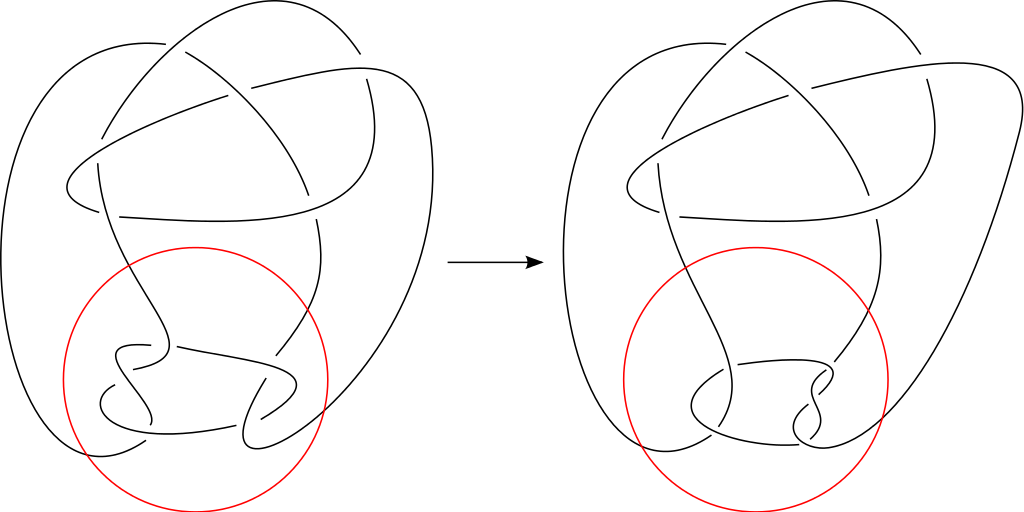
\includegraphics[width=0.601\linewidth]{../data/mixed/knudemutation.png}
    \caption{Węzły $11n_{42}$ oraz $11n_{34}$. Grafika Sørena Jørgensena, dostępna na licencji \href{https://creativecommons.org/licenses/by-sa/3.0/deed.en}{CC BY-SA 3.0} pod adresem \url{https://en.wikipedia.org/wiki/File:Knudemutation.svg}.}
\end{figure}
    
Niedawno Stojmenow podjął się systematycznie szukania mutantów wśród węzłów o~mniej niż 19 skrzyżowaniach (praca \cite{stoimenow2010} z~2010 roku).
\index[persons]{Stojmenow, Aleksander}%
Początkowo pracował sam, badając pewne subtelne przykłady postanowił uwikłać w swój projekt Toshifumiego Tanakę, a później także Daniela Mateię.
\index[persons]{Tanaka, Toshifumi}%
\index[persons]{Daniel, Matei}%
Praca \cite{stoimenow2010} jest kontynuacją artykułu, który napisali wspólnymi siłami.

I tak na stronie 531 można przeczytać, że ,,niezmienniki Wasiljewa co najwyżej 8. stopnia nie rozróżniają mutantów węzłów \cite{chmutov1994}'', ja tego nie widzę.
\index{niezmiennik!Wasiljewa}%
Mniej więcej sześć lat później wynik poprawił J. Murakami (nie mylić z H. Murakamim!) do 10. stopnia w~niezindeksowanej pracy \cite{murakami1999}.
\index[persons]{Murakami, Jun}
W międzyczasie Cromwell, Morton znaleźli niezmiennik stopnia 11., który odróżnia węzły Conwaya oraz Kinoshity-Terasakiego; patrz \cite{cromwell1996}.
\index[persons]{Cromwell, Peter}%
\index[persons]{Morton, Hugh}%
% czy Murakami potwierdził wynik Cromwella, Mortona?

Mutant węzła złożonego także jest złożony, co więcej istnieje bijekcja między czynnikami w ich rozkładach na węzły pierwsze Ruberman -- \cite{ruberman1987}.
\index[persons]{Ruberman, Daniel}%
Dzięki temu możemy bez straty ogólności założyć, że badamy tylko węzły pierwsze, niestety wciąż nie jest znana ogólna procedura pozwalająca wyliczyć wszystkie mutanty danego węzła.

Zaraz po rewolucji, jaką w latach 80. wywołała relacja kłębiasta, Ewing napisał z~Millettem komputerowy program w~języku C, który wyjątkowo szybko znajdował wielomiany HOMFLY oraz Kauffmana zadanego węzła.
\index[persons]{Ewing, Bruce}%
\index[persons]{Millett, Kenneth}%
Nawet dziś program ten jest w stanie uporać się z węzłami, z którymi nie radzą sobie inne narzędzia.
Autorzy nie wiedzieli wtedy, że ktoś jeszcze będzie z nich korzystać w przyszłości, dlatego poczynili w kodzie liczne optymalizacje dla stacji roboczej Sun, jaką wtedy dysponowali.
Dzisiaj okazuje się, że dla węzłów o większej liczbie skrzyżowań program często kończy swoje działanie zrzutem pamięci, wpada w pętlę bez wyjścia albo zwraca niepoprawny wynik (składniki wielomianu Kauffmana są postaci $a^m z^n$, gdzie $m + n$ jest nieparzyste).
Stojmenow korzystał z tych programów podczas tablicowania mutantów.
Jak postępował?
\begin{enumerate}
    \item podzielił węzły na grupy o tej samej objętości, wielomianie Jonesa oraz Alexandera;
    \item w każdej z grup szukał ciągu mutacji pomiędzy diagramami minimalnymi;
    \item tam, gdzie nie udało się znaleźć mutantów, liczył 2-kablowy wielomian HOMFLY;
    \item jeśli wielomian był taki sam, szukał ciągu mutacji między nieminimalnymi diagramami do 18 skrzyżowań;
    \item wreszcie pozostałe grupy zostały potraktowane reprezentacjami grupy podstawowej dwukrotnego nakrycia.
\end{enumerate}

Podsumowanie jego pracy zawiera tabela:

\begin{table}[H]
    \centering
    \begin{tabular}{lccccc} \toprule
        skrzyżowania & 11 & 12 & 13  & 14   & 15    \\ \midrule
        pary         & 16 & 70 & 703 & 3917 & 24884 \\
        trójki       &    & 5  & 38  & 233  & 1000  \\
        czwórki      &    &    & 32  & 262  & 2909  \\
        szóstki      &    &    & 1   & 17   & 172   \\
        ósemki       &    &    &     & 6    & 84    \\
        łącznie      & 16 & 75 & 774 & 4435 & 29049 \\
        \bottomrule
        \hline
    \end{tabular}
    \caption{Liczba grup mutantów wśród pierwszych węzłów do 15 skrzyżowań}
\end{table}

\subsubsection{Rozróżnianie mutantów}
Żaden wielomianowy niezmiennik opisany w~tej książce nie potrafi odróżnić od siebie węzłów $11n_{34}$ oraz $11n_{42}$.
Okazuje się, że niewielomianowe niezmienniki też często są bezradne.

\begin{proposition}
    Mutacja węzła nie zmienia jego wielomianu Alexandera.
\index{wielomian!Alexandera}%
\end{proposition}

% w commicie 1fe48ad183cb592e897f4151f9c18439baa84274 wymieniam:
% +    kablowego wielomianu Jonesa, % menasco91
% +    2-kablowego wielomianu HOMFLY, % przytycki89
% +    kablowego wielomianu Kauffmana, % lipson87
% +    sygnatury Tristrama-Levine'a, % cooper99
% +    symplicjalnEj objętości Gromowa, % ruberman87
% +    instanton homologii Floera, % ruberman99
% +    niezmienników Wittena % rong94
% +    ani Cassona. % kirk89
% ale teraz nie potrafię sobie przypomnieć, jak znalazłem te niezmienniki/prace. :(
% wydaje mi się, że źródłem nie jest stoimenow10, może Math Overflow?

\begin{proof}
    Stojmenow, Tanaka \cite[s. 1]{tanaka2009} piszą, że to proste ćwiczenie teorii kłębiastej, oraz że rozumowanie łatwo przenosi się na odkryte później wielomiany Jonesa, HOMFLY, BLM/Ho, Kauffmana.
\end{proof}

Warto przytoczyć teraz obserwację 3.8.2 z \cite[s. 43]{kawauchi1996} pochodzącą tak naprawdę z pracy Viro \cite{viro1973}: niech sploty $L_1, L_2$ będą mutantami, wtedy podwójne przestrzenie nakryciowe nad $S^3$ rozgałęzione wzdłuż $L_1$ albo $L_2$ są homeomorficzne z zachowaniem orientacji.
Cooper \cite{cooper1982} zauważył, że macierze Seiferta mutantów są $S$-równoważne.
\index{macierz!Seiferta}%
To tłumaczy czemu większość niezmienników nie radzi sobie z odróżnianiem mutantów.
% Viro: Two-fold branched coverings of three-sphere

% z tanaka09
Wzór kablowy\footnote{Niech $T$ będzie trywialnym torusem, zawierającym węzeł $K$, zaś $e \colon T \to S^3$ włożeniem $T$ na otoczenie węzła $C$ tak, że $e$ przenosi równoleżnik $T$ na równoleżnik $C$. Wtedy $\alexander_{eK} (t) = \alexander_K(t)\alexander_C(t^n)$.} \cite[tw. 6.15]{lickorish1997} pokazuje, że wielomian Alexandera nie odróżnia satelitów zmutowanych węzłów.
Wielomian Jonesa nie spełnia żadnego wzoru kablowego (gdyż czasami odróżnia kable węzłów o~tym samym wielomianie), ale…
\index{wzór!kablowy}%

\begin{proposition}
    Mutacja węzła nie zmienia jego kablowego wielomianu Jonesa.
\index{wielomian!Jonesa}%
\end{proposition}

\begin{proof}
\index[persons]{Morton, Hugh}%
\index[persons]{Traczyk, Paweł}%
    Morton, Traczyk \cite{traczyk1988}.
    % kiedyś tu było niezdefiniowane menasco91 = Menasco, Thistlethwaite: The Tait flyping conjecture, ale w 2022 roku przeczytałem Stoimenow: Tabulating and distinguishing mutants zmieniłem zdanie: "nonetheless Morton and Traczyk [36] showed that..."
\end{proof}

Praca \cite{traczyk1988} wspomina jeszcze, że to samo jest prawdą także dla ,,wielomianu Jonesa dwóch zmiennych'' (HOMFLY) i 2-kabli, ale nie dla dowolnych satelitów.
Fakt, że wielomian HOMFLY (a także Kauffmana) nie odróżniają 2-satelitów mutantów, odkryto rok wcześniej:

\begin{proposition}
\label{mutants_and_homfly}%
\index{wielomian!HOMFLY}%
    Mutacja węzła nie zmienia jego 2-kablowego wielomianu HOMFLY.
\end{proposition}

\begin{proof}
\index[persons]{Lickorish, William}%
\index[persons]{Lipson, Andrew}%
\index[persons]{Przytycki, Józef}%
    Lickorish, Lipson \cite{lipson1987}, później też Przytycki \cite{przytycki1989}.
    % TODO: skąd to o Przytyckim???
\end{proof}

Lepiej jest z~3-kablami: wielomian HOMFLY odróżnia tak węzły Kinoshity-Terasakiego i~Conwaya, ale wymaga takiej ilości rachunków, że mało komu chce się je przeprowadzać dla innych węzłów.
\index{węzeł!Conwaya}%
\index{węzeł!Kinoshity-Terasakiego}%

\begin{proposition}
    Mutacja węzła nie zmienia jego (2-?)kablowego wielomianu Kauffmana.
\index{wielomian!kablowy}%
\index{wielomian!Kauffmana}%
\end{proposition}

\begin{proof}
\index[persons]{Lickorish, William}%
\index[persons]{Lipson, Andrew}%
    Lickorish, Lipson \cite{lipson1987}.
\end{proof}

Morton w recenzji pracy Lickorisha, Lipsona wspomina, że dla satelitów owijających się więcej niż $2$ razy to nie jest prawda, jak później odkryto.

\begin{proposition}
\index{wielomian!BLM/Ho}%
    Mutacja węzła nie zmienia jego wielomianu BLM/Ho.
\end{proposition}

\begin{proof}
    \cite{tanaka2009}, choć nie wiemy, gdzie dokładnie.
\end{proof}

\begin{proposition}
\index{sygnatura!Levine'a-Tristrama}%
    Mutacja węzła nie zmienia jego sygnatury Levine'a-Tristrama.
\end{proposition}

\begin{proof}
\index[persons]{Cooper, Daryl}%
\index[persons]{Lickorish, William}%
    Cooper, Lickorish w~\cite{cooper1999} podają klasyczny dowód, że mutacja zachowuje wielomian Alexandera, oparty o~macierz Seiferta.
    Wiedząc, jak wygląda ta macierz, autorzy wyciągają wniosek, że sygnatura splotów (!) w~homologicznej 3-sferze też jest zachowywana.
\end{proof}

\begin{proposition}
\index{objętość!symplicjalna Gromowa}%
\label{mutants_the_same_volume}%
    Mutacja węzła nie zmienia jego symplicjalnej objętości Gromowa.
\end{proposition}

\begin{proof}
\index[persons]{Ruberman, Daniel}%
    Ruberman \cite{ruberman1987}.
    % Ruberman [42] showed that mutants have equal volume in all hyperbolic pieces of the JSJ decomposition.
\end{proof}

\begin{proposition}
\index{homologia!Floera}%
    Mutacja węzła nie zmienia jego instanton homologii Floera.
\end{proposition}

\begin{proof}
\index[persons]{Ruberman, Daniel}%
    Jeszcze raz Ruberman \cite{ruberman1999}.
\end{proof}

\begin{proposition}
\index{niezmiennik!Wittena}%
    Mutacja węzła nie zmienia jego niezmienników Wittena.
\end{proposition}

\begin{proof}[Niedowód]
    Rong \cite{rong1994}: niech $L$ będzie obramowanym splotem w~3-rozmaitości $M$, zaś $F \subseteq M$ dwustronną powierzchnią, tnącą splot w 0, 1 lub 4 (transwersalnie) punktach, o genusie $g = 0$, $1$ lub $2$, wtedy rozcięcie $M$ wzdłuż $F$ i sklejenie po obrocie o 180 stopni daje parę $(M^\tau, K^\tau)$, która ma ten sam niezmiennik Wittena w $\mathrm{SU}(2)$ jak wyjściowa para $(M, K)$.
    % TODO: dla wybranych mutacji
\end{proof}

\begin{proposition}
\index{niezmiennik!Cassona}%
    Mutacja węzła nie zmienia jego niezmienników Cassona.
\end{proposition}

Celowo nie podajemy definicji tego niezmiennika.
Nieformalnie, zlicza on co drugą klasę sprzężoności reprezentacji grupy podstawowej homologicznej 3-sfery w grupie $SU(2)$.

\begin{proof}
\index[persons]{Kirk, Paul}%
    Kirk \cite{kirk1989}.
\end{proof}

\begin{conjecture}
    Mutacja węzła nie zmienia jego liczby gordyjskiej.
\end{conjecture}

Jak czytamy w \cite[problem 1.69]{kirby1978}, przypuszczenie to jest bardzo trudne do udowodnienia, bo wynikałaby z niego bardzo stara hipoteza \ref{conjecture_unknotting_additive}, że liczba gordyjska splotów jest addytywna.
\index{hipoteza!o liczbie gordyjskiej}%
Przytoczymy dwa częściowe wyniki.
Najpierw Rolfsen \cite{rolfsen1993} zauważył, że jedynym mutantem niewęzła jest sam niewęzeł.
\index[persons]{Rolfsen, Dale}%
Dekadę później Gordon, Luecke \cite{gordon2006} pokazali, iż klasa węzłów $1$-gordyjskich jest zamknięta na przeprowadzanie mutacji.
\index[persons]{Gordon, Cameron}%
\index[persons]{Luecke, John}%
(Ohtsuki \cite[problem 12.15]{ohtsuki2002} powtarza hipotezę.)
\index[persons]{Ohtsuki, Tomotada}%

% to NIE jest z stoimenow10
\begin{proposition}
    Niech $D$ będzie alternującym diagramem.
    Wtedy każdy mutant $D$ też jest alternujący.
\end{proposition}

Wśród niezmienników, które mutacja czasami zmienia, znajduje się genus plastrowy:

\begin{proposition}
\index{genus!plastrowy}%
    Niech $m, n$ będą nieujemnymi liczbami całkowitymi.
    Wtedy istnieje węzeł $K$ o genusie plastrowym równym $m$, którego pewien mutant ma genus plastrowy równy $n$.
\end{proposition}

Stanowi to uogólnienie obserwacji Livingstona \cite{livingston1983}, że istnieją mutanty o~różnym genusie plastrowym.
\index[persons]{Livingston, Charles}%

\begin{proof}
    Kim, Livingston w \cite{kim2005}.
\end{proof}

Zbiór problemów niskowymiarowej topologii opublikowany przez Kirby'ego \cite{kirby1978} zawiera następujące pytanie:
\index[persons]{Kirby, Rob}%

\begin{conjecture}[problem 1.91]
\index{węzeł!satelitarny}
    Niech $K$ będzie prostym węzłem bez orientacji (w jego dopełnieniu nie ma nierównoległych do brzegu, nieściśliwych pierścieni).
\index{nieściśliwy}%
    Czy istnieją węzły niebędące mutantami $K$, których nie można odróżnić od $K$ wielomianem Jonesa oraz wszystkimi jego satelitami?
\end{conjecture}

Stojmenow pisze, że tak: pierwszą chronologicznie parą jest $14_{41721}$, $14_{42125}$, dowód opiera się na wzorze fuzyjnym Masbauma-Vogela z~pracy \cite{masbaum1994}.
\index[persons]{Stojmenow, Aleksander}
\index[persons]{Masbaum, Gregor}%
\index[persons]{Vogel, Pierre}%
\index{wzór!fuzyjny Masbauma-Vogela}%
Patrz \cite[przykład 3.3]{tanaka2009} oraz \cite[przykład 3.2]{stoimenow2010}.

Choć wzór ten zastosowany do konkretnej pary węzłów sprawia zazwyczaj trudności rachunkowe, to jest wystarczającym narzędziem, by rozszerzyć konstrukcję do ogólnego wyniku:

\begin{proposition}
    Istnieje nieskończenie wiele par prostych węzłów hiperbolicznych o tych samych kolorowych wielomianach Jonesa, które nie są swoimi mutantami.
\end{proposition}

\begin{proof}
    Stojmenow, Tanaka \cite[tw. 1.1]{tanaka2009}.
\end{proof}

\index{mutant|)}




\section{Precle}
\index{węzeł!preclowy|see {precel}}%
\index{precel|(}%
Precle to sploty ze standardowym diagramem, na którym wyróżnić można co najmniej trzy warkocze na dokładnie dwóch pasmach.
Warkocze te ułożone są w sposób cykliczny.
Pojawiły się po raz pierwszy w~książce Reidemeistera z~1932 roku jako przykład węzła o~trywialnym wielomianie Alexandera.
Zanim podamy formalną definicję, wygodnie będzie przyjrzyć się ogólniejszej rodzinie splotów Montesinosa, nazwanych tak na cześć José Marii Montesinosa Amilibii, topologa hiszpańskiego.
\index[persons]{Montesinos, José}%
Wprowadził je do matematyki w~1973 roku \cite{montesinos73}.

Kawauchi \cite[s. 29]{kawauchi96} pisze, że Montesinos uogólnił precle, bo dwukrotne nakrycie nad $S^3$ rozgałęzione wzdłuż precla jest rozmaitością Seiferta.
\index{rozmaitość Seiferta}%

\index{splot!Montesinosa|(}%
\begin{definition}[splot Montesinosa]
    Splotem Montesinosa nazywamy splot o~poniższym diagramie, gdzie wymierne liczby $\alpha_i/\beta_i$ oraz całkowita $e \in \Z$ odpowiadają supłom.
\begin{comment}
    \[
    \begin{tikzpicture}[baseline=-0.65ex, scale=0.1]
    %\useasboundingbox (-5, -9) rectangle (5, 5);
        \draw[semithick] (-5, 5) rectangle (5, 15);
        \foreach \x in {0,1,3,4} {
            \draw[semithick] (15*\x-35, -15) rectangle (15*\x-25, -5);
        }
        \foreach \x in {0,1,2,3,4,5} {
            \draw[semithick] (15*\x-35, -8) to (15*\x-40, -8);
            \draw[semithick] (15*\x-35, -12) to (15*\x-40, -12);
        }
        \draw[semithick] (-40, -8) [in=down, out=left] to (-45, -3);
        \draw[semithick] (-40, -12) [in=down, out=left] to (-49, -3);

        \draw[semithick] (-40, 8) [in=up, out=left] to (-45, 3);
        \draw[semithick] (-40, 12) [in=up, out=left] to (-49, 3);

        \draw[semithick] (40, 8) [in=up, out=right] to (45, 3);
        \draw[semithick] (40, 12) [in=up, out=right] to (49, 3);

        \draw[semithick] (40, -8) [in=down, out=right] to (45, -3);
        \draw[semithick] (40, -12) [in=down, out=right] to (49, -3);

        \draw[semithick] (-45, -3)  to (-45, 3);
        \draw[semithick] (-49, -3)  to (-49, 3);
        \draw[semithick] (45, -3)  to (45, 3);
        \draw[semithick] (49, -3)  to (49, 3);

        \draw[semithick] (-5, 8)  to (-40, 8);
        \draw[semithick] ( 5, 8)  to ( 40, 8);
        \draw[semithick] (-5, 12)  to (-40, 12);
        \draw[semithick] ( 5, 12)  to ( 40, 12);

        \node at (0, 10) {e};
        \node at (0, -10) {\ldots};
        \node at (-15, -10) {$\displaystyle \frac{\alpha_2}{\beta_2}$};
        \node at (-30, -10) {$\displaystyle \frac{\alpha_1}{\beta_1}$};
        \node at (15, -10) {$\displaystyle \frac{\alpha_{n-1}}{\beta_{n-1}}$};
        \node at (30, -10) {$\displaystyle \frac{\alpha_n}{\beta_n}$};
    \end{tikzpicture}
    \]
\end{comment}
\end{definition}

Cały dwunasty rozdział podręcznika Burdego i~Zieschanga \cite{burde14} jest poświęcony splotom Montesinosa.
Można tam znaleźć ich klasyfikację, zawiera jednak pułapkę: autorzy używają innej notacji dla supłów dwumostowych.
Podają przykład węzła $43/105 = [0, 2, 2, 3, 1, 4]$, dla nas to jest $105/22 = [4, 1, 3, 2, 2]$.

\begin{proposition}
    Sploty Montesinosa o $r \ge 3$ supłach $\beta_1/\alpha_1, \beta_2/\alpha_2, \ldots$ takich, że
    \begin{equation}
        \sum_{j=1}^r \frac{1}{\alpha_j} \le r - 2
    \end{equation}
    są sklasyfikowane (z dokładnością do cyklicznych permutacji oraz odwracania) przez uporządkowany zbior ułamków $\{\beta_i/\alpha_i \mod 1 : 1 \le i \le r\}$ razem z~wymierną liczbą
    \begin{equation}
        e_0 = e + \sum_{j=1}^r \frac{\beta_j}{\alpha_j}.
    \end{equation}
\end{proposition}

Powyższy fakt nie używa naszej notacji!

\begin{proof}
\index[persons]{Bonahon, Francis}%
    Praca doktorska Bonahona \cite{bonahon79}.
    W~internecie dostępny jest jej skan (gdyż była pisana odręcznie po francusku!), ale angielskie tłumaczenie nie istnieje.
\end{proof}

Używając nadal tej niestandardowej notacji można sklasyfikować węzły odwracalny czy zwierciadlane:

\begin{proposition}
\index{węzeł!zwierciadlany}%
    Splot Montesinosa jest zwierciadlany wtedy i tylko wtedy, gdy $e = 0$ oraz istnieje permutacja $\pi$, cykl długości $r$ lub odwrócenie, taka że
    \begin{equation}
        \frac{\beta_{\pi(i)}}{\alpha_{\pi(i)}} \equiv -\frac{\beta_i}{\alpha_i} \pmod 1
    \end{equation}
\end{proposition}

\begin{proof}
    Burde, Zieschang, Heusener \cite[s. 230]{burde14}.
\end{proof}

\begin{corollary}
    Splot Montesinosa z nieparzystą liczbą supłów nie jest zwierciadlany.
\end{corollary}

\begin{proposition}
\index{węzeł!odwracalny}%
    Splot Montesinosa jest odwracalny wtedy i tylko wtedy, gdy, po ewentualnej zmianie etykiet supłów, przynajmniej jedna z liczb $\alpha_i$ jest parzysta lub wszystkie liczby $\alpha_i$ są parzyste, a sam splot ma postać
    \begin{equation}
        M(e_0, \beta_1/\alpha_1, \ldots, \beta_p/\alpha_p, \beta_p/\alpha_p, \ldots, \beta_1/\alpha_1)
    \end{equation}
    (oraz $r = 2p$) lub
    \begin{equation}
        M(e_0, \beta_1/\alpha_1, \ldots, \beta_p/\alpha_p, \beta_{p+1}/\alpha_{p+1}, \beta_p/\alpha_p, \ldots, \beta_1/\alpha_1)
    \end{equation}
    (oraz $r = 2p+1$) lub
    \begin{equation}
         M(e_0, \beta_1/\alpha_1, \ldots, \beta_p/\alpha_p, \beta_{p+1}/\alpha_{p+1}, \beta_p/\alpha_p, \ldots, \beta_2/\alpha_2).
    \end{equation}
    (oraz $r = 2p$).
\end{proposition}

\begin{proof}
    Burde, Zieschang, Heusener \cite[s. 231]{burde14}.
\end{proof}

\index{splot!Montesinosa|)}%

% DICTIONARY;pretzel;preclowy;węzeł
\begin{definition}[precel]
\label{def:pretzel}%
    Splot Montesinosa o~całkowitych współczynnikach nazywamy preclem.
\end{definition}

Na standardowym diagramie precla $(p_1, p_2, \ldots, p_n)$ występuje $p_1$ lewych skrzyżowań w~pierwszym suple, $p_2$ w~drugim, i~tak dalej.
Taki precel jest węzłem dokładnie wtedy, gdy $n$ oraz $p_i$ są nieparzyste lub dokładnie jedna z~liczb $p_i$ jest parzysta (\cite[s. 27]{kawauchi96}).

\begin{proposition}
    Jeśli co najmniej dwa współczynniki $p_i, p_j$ zerują się, precel jest rozszczepialny.
\end{proposition}

\begin{proof}
    Widać to bezpośrednio z diagramu: jego część zawarta między supłem $p_i$ oraz $p_j$ jest rozłączna z~resztą diagramu.
    Nie jest jednak prawdziwa implikacja odwrotna.
    % TODO: podać przykład
\end{proof}

Precel $(1,1,1)$ to prawy trójlistnik, $(5, -1, -1)$ to węzeł dokerski $6_1$, $(-3, 0, -3)$ to splot dwóch trójlistników, zaś $(2p, 2q, 2r)$ jest splotem trzech niewęzłów.
Precle $(-2, 3, 2n+1)$ są szczególnie użyteczne jako narzędzie do badania 3-rozmaitości.
Wiele twierdzeń, które dotyczą takich rozmaitości, opiera się na przykład na chirurgii Dehna precla $(-2, 3, 7)$.
\index{chirurgia Dehna}%
\index{precel!(-2, 3, 7)}%

\begin{proposition}
\index{węzeł!torusowy}%
    Niech $K$ będzie węzłem torusowym.
    Jeśli $K$ jest jednocześnie $(-2, 3, k)$-preclem, to
    \begin{equation}
        K = 5_{1} = T_{2,5} = P(1, 3, -2)
    \end{equation}
    albo
    \begin{equation}
        K = 8_{19} = T_{3,4} = P(3, 3, -2)
    \end{equation}
    albo
    \begin{equation}
        K = 10_{124} = T_{3,5} = P(5, 3, -2).
    \end{equation}
\end{proposition}

\begin{proof}
\index[persons]{Garoufalidis, Stavros}%
\index[persons]{Koutschan, Christoph}%
    Garoufalidis, Koutschan \cite{garoufalidis12}.
\end{proof}

\begin{proposition}
    \label{prp:pretzel_not_invertible}
    Niech $p, q, r$ będą liczbami nieparzystymi takimi, że $|p|, |q|, |r|$ są parami różne i większe niż $1$.
    Wtedy $(p, q, r)$-precel jest nieodwracalny.
\end{proposition}

\begin{proof}
\index[persons]{Fox, Ralph}%
\index[persons]{Trotter, Hale}%
    Zgodnie z sugestią Foxa, Trotter przetłumaczył problem na język teorii grup w \cite{trotter63}.
    Wyróżnia w~grupie węzła dwa elementy -- (zorientowany) południk i równoleżnik.
    Jeśli dwa węzły są równoważne, to homeomorfizm $\R^3 \to \R^3$ posyłający jeden na drugi wyznacza izomorfizm ich grup podstawowych, który posyła południk na południk i równoleżnik na równoleżnik.
    W szczególności, jeśli węzeł jest odwracalny, to jego grupa posiada specjalny automorfizm (,,inwersję'') odwracający zarówno południk, jak i równoleżnik.
    To prowadzi do sprzeczności w przypadku rozpatrywanych precli.
\end{proof}

Wystarczający warunek z tego stwierdzenia jest prawie konieczny.
Jeśli $p = r$, węzeł można odwrócić przez półobrót wokół środkowej osi.
Cykliczne permutacje trójki $(p, q, r)$ nie zmieniają węzła, więc wszystkie trzy liczby $p, q, r$ muszą być różne.
Jeśli jedna z tych liczb jest parzysta, półobrót wokół poziomej osi odwraca węzeł.
Z pracy Bankwitza i Schumanna wynika, że jeśli któryś z parametrów ma wartość $\pm 1$, to węzeł też jest odwracalny.
\index[persons]{Bankwitz, Carl}%
\index[persons]{Schumann, Hans}%
% Bankwitz, Carl; Schumann, Hans Georg;
% Über viergeflechte. (German)
% Abh. Math. Sem. Univ. Hamburg 10 (1934), no. 1, 263–284.
Nie jest trudno pokazać to wprost.
Zatem nie wiemy jedynie jakie są precle $(p, q, -q)$, gdzie $|p| \neq |q|$ oraz $|p|, |q| \ge 3$.

Jeśli liczby $p, q, r$ są nieparzyste i tego samego znaku, to wyznacznik precla $(p, q, r)$ jest postaci $4n+3$.
\index{wyznacznik}%
Wtedy używając formy kwadratowej (jak Reidemeister w 1932!) można pokazać, że taki węzeł nie jest achiralny.
Niech $K$ będzie zorientowanym preclem $(3, 5, 7)$.
Wtedy $K$, $mK$, $rK$, $mrK$ są parami nierównoważne.
Węzeł $K \shrap mK$ jest dodatnio zwierciadlany, zaś $rK \shrap mK$ ujemnie zwierciadlany.
Trójlistnik jest odwracalny, ale nie zwierciadlany, ósemka jest zwierciadlana i~odwracalna.
To pokazuje, że wszystkie typy symetrii są realizowane przez precle lub sumy precli.

\begin{proposition}
\label{prp:pretzel_alexander}%
\index{wielomian!Alexandera}%
    Jeżeli liczby $p, q, r$ są nieprzyste, to wielomianem Alexandera $(p, q, r)$-precla jest
    \begin{equation}
        \alexander = \frac 14 ((pq+qr+pr) (t-1)^2 + (t+1)^2).
    \end{equation}
\end{proposition}

\begin{proof}
\index[persons]{Bae, Yongju}%
\index[persons]{Lee, In}%
    Bae, Lee pokazali w \cite[lemat 3.1]{bae20}, że macierz Seiferta $(p, q, r)$-precla to
    \begin{equation}
        M = \frac 1 2 \begin{bmatrix}
            p+q & p-1 \\
            p+1 & p+r
        \end{bmatrix},
    \end{equation}
    wystarczy więc użyć wzoru $\alexander = \det(M-tM^t)$.
\end{proof}

Wielomian Alexandera precla $(p_1, \ldots, p_n)$ nigdy nie zależy od kolejności współczynników, jest to ćwiczenie w~książce Livingstona \cite[s. 215]{livingston93}.

\begin{proposition}
\index{kolorowalność}%
    Niech $n$ będzie liczbą pierwszą.
    Węzeł $p, q, r$-preclowy jest $n$-kolorowalny wtedy i~tylko wtedy, gdy $n$ dzieli $|pq+qr+pr|$.
    Jeśli przynajmniej jedna z~liczba $p, q, r$ nie jest wielokrotnością $n$, kolorowanie z dokładnością do permutacji jest jedyne.
    W przeciwnym przypadku istnieją cztery różne kolorowania.
\end{proposition}

\begin{proof}
\index[persons]{Brownell, Kathryn}%
\index[persons]{O'Neil, Kaitlyn}%
\index[persons]{Taalman, Laura}%
    Pierwsza część jest wnioskiem ze stwierdzeeń \ref{prp:colour_determinant}, \ref{prp:alexander_determinant} oraz \ref{prp:pretzel_alexander}.
    Dowód drugiej zawiera praca Brownell, O'Neil, Taalman \cite{taalman05}, trzech Amerykanek.
\end{proof}

Podano tam także ogólny wzór na liczbę $n$-kolorowań dowolnego węzła.

\index{precel|)}%

% Koniec sekcji Precle


\todo[inline]{\url{https://en.wikipedia.org/wiki/Lissajous_knot}}

\chapter{Tablice węzłów pierwszych}
\section{Wartości niezmienników}
\label{sec:table_of_invariants}
Tabela przedstawia węzły pierwsze o~co najwyżej dziesięciu skrzyżowaniach oraz wartości ich niezmienników (całkowitoliczbowych lub wielomianowych).
Zgodnie z~oznaczeniami przyjętymi w reszcie książki, $\operatorname{u}, \operatorname{b}, \operatorname{br}$ to kolejno liczba gordyjska, warkoczowa i~mostowa.
Zapis $2..3$ mówi, że dokładna wartość nie jest znana i leży w przedziale $[2,3]$.
Jeśli liczba mostowa wynosi dokładnie $2$, zamiast niej podajemy nieskracalny ułamek $p/q$, który koduje węzeł.
Dalej, $\det$ jest wyznacznikiem, $\sigma$ sygnaturą, Arf -- oczywiście niezmiennikiem Arfa.
Wielomian Conwaya $\nabla(z)$ dla oszczędności miejsca podajemy jako ciąg współczynników, na przykład $1-1$ jest skrótem od $1-z^2$.

Dane zawarte w~tej tabeli pochodzą ze strony \url{http://www.indiana.edu/~knotinfo/}.
Jej autorzy, Chuck Livingston z~uniwersytetu Indiany  oraz Jae Choon Cha (z koreańskiego Pohangu) prezentują tam wiele innych niezmienników.

\renewcommand*{\arraystretch}{1.4}
\footnotesize
\begin{longtable}{lccccccllc}
\hline
nazwa & u~& b & br & $\det$ & sygn. & Arf & $\nabla(z)$ & sym. & alt. \\ \hline
\endhead % all the lines above this will be repeated on every page
$3_{1}$     &  $1$     &  $2$  &  $3/1$    &  $3$    &  $-2$  &  $1$  &  $1+1$          &  odwracalny  &  tak  \\
$4_{1}$     &  $1$     &  $3$  &  $5/2$    &  $5$    &  $0$   &  $1$  &  $1-1$          &  całkowicie  &  tak  \\
$5_{1}$     &  $2$     &  $2$  &  $5/1$    &  $5$    &  $-4$  &  $1$  &  $1+3+1$        &  odwracalny  &  tak  \\
$5_{2}$     &  $1$     &  $3$  &  $7/3$    &  $7$    &  $-2$  &  $0$  &  $1+2$          &  odwracalny  &  tak  \\
$6_{1}$     &  $1$     &  $4$  &  $9/7$    &  $9$    &  $0$   &  $0$  &  $1-2$          &  odwracalny  &  tak  \\
$6_{2}$     &  $1$     &  $3$  &  $11/4$   &  $11$   &  $-2$  &  $1$  &  $1-1-1$        &  odwracalny  &  tak  \\
$6_{3}$     &  $1$     &  $3$  &  $13/5$   &  $13$   &  $0$   &  $1$  &  $1+1+1$        &  całkowicie  &  tak  \\
$7_{1}$     &  $3$     &  $2$  &  $7/1$    &  $7$    &  $-6$  &  $0$  &  $1+6+5+1$      &  odwracalny  &  tak  \\
$7_{2}$     &  $1$     &  $4$  &  $11/5$   &  $11$   &  $-2$  &  $1$  &  $1+3$          &  odwracalny  &  tak  \\
$7_{3}$     &  $2$     &  $3$  &  $13/9$   &  $13$   &  $-4$  &  $1$  &  $1+5+2$        &  odwracalny  &  tak  \\
$7_{4}$     &  $2$     &  $4$  &  $15/11$  &  $15$   &  $-2$  &  $0$  &  $1+4$          &  odwracalny  &  tak  \\
$7_{5}$     &  $2$     &  $3$  &  $17/7$   &  $17$   &  $-4$  &  $0$  &  $1+4+2$        &  odwracalny  &  tak  \\
$7_{6}$     &  $1$     &  $4$  &  $19/7$   &  $19$   &  $-2$  &  $1$  &  $1+1-1$        &  odwracalny  &  tak  \\
$7_{7}$     &  $1$     &  $4$  &  $21/8$   &  $21$   &  $0$   &  $1$  &  $1-1+1$        &  odwracalny  &  tak  \\
$8_{1}$     &  $1$     &  $5$  &  $13/11$  &  $13$   &  $0$   &  $1$  &  $1-3$          &  odwracalny  &  tak  \\
$8_{2}$     &  $2$     &  $3$  &  $17/6$   &  $17$   &  $-4$  &  $0$  &  $1+0-3-1$      &  odwracalny  &  tak  \\
$8_{3}$     &  $2$     &  $5$  &  $17/4$   &  $17$   &  $0$   &  $0$  &  $1-4$          &  całkowicie  &  tak  \\
$8_{4}$     &  $2$     &  $4$  &  $19/14$  &  $19$   &  $2$   &  $1$  &  $1-3-2$        &  odwracalny  &  tak  \\
$8_{5}$     &  $2$     &  $3$  &  $3$      &  $21$   &  $-4$  &  $1$  &  $1-1-3-1$      &  odwracalny  &  tak  \\
$8_{6}$     &  $2$     &  $4$  &  $23/10$  &  $23$   &  $-2$  &  $0$  &  $1-2-2$        &  odwracalny  &  tak  \\
$8_{7}$     &  $1$     &  $3$  &  $23/9$   &  $23$   &  $2$   &  $0$  &  $1+2+3+1$      &  odwracalny  &  tak  \\
$8_{8}$     &  $2$     &  $4$  &  $25/9$   &  $25$   &  $0$   &  $0$  &  $1+2+2$        &  odwracalny  &  tak  \\
$8_{9}$     &  $1$     &  $3$  &  $25/7$   &  $25$   &  $0$   &  $0$  &  $1-2-3-1$      &  całkowicie  &  tak  \\
$8_{10}$    &  $2$     &  $3$  &  $3$      &  $27$   &  $2$   &  $1$  &  $1+3+3+1$      &  odwracalny  &  tak  \\
$8_{11}$    &  $1$     &  $4$  &  $27/10$  &  $27$   &  $-2$  &  $1$  &  $1-1-2$        &  odwracalny  &  tak  \\
$8_{12}$    &  $2$     &  $5$  &  $29/12$  &  $29$   &  $0$   &  $1$  &  $1-3+1$        &  całkowicie  &  tak  \\
$8_{13}$    &  $1$     &  $4$  &  $29/11$  &  $29$   &  $0$   &  $1$  &  $1+1+2$        &  odwracalny  &  tak  \\
$8_{14}$    &  $1$     &  $4$  &  $31/12$  &  $31$   &  $-2$  &  $0$  &  $1+0-2$        &  odwracalny  &  tak  \\
$8_{15}$    &  $2$     &  $4$  &  $3$      &  $33$   &  $-4$  &  $0$  &  $1+4+3$        &  odwracalny  &  tak  \\
$8_{16}$    &  $2$     &  $3$  &  $3$      &  $35$   &  $2$   &  $1$  &  $1+1+2+1$      &  odwracalny  &  tak  \\
$8_{17}$    &  $1$     &  $3$  &  $3$      &  $37$   &  $0$   &  $1$  &  $1-1-2-1$      &  ujemny      &  tak  \\
$8_{18}$    &  $2$     &  $3$  &  $3$      &  $45$   &  $0$   &  $1$  &  $1+1-1-1$      &  całkowicie  &  tak  \\
$8_{19}$    &  $3$     &  $3$  &  $3$      &  $3$    &  $-6$  &  $1$  &  $1+5+5+1$      &  odwracalny  &  nie  \\
$8_{20}$    &  $1$     &  $3$  &  $3$      &  $9$    &  $0$   &  $0$  &  $1+2+1$        &  odwracalny  &  nie  \\
$8_{21}$    &  $1$     &  $3$  &  $3$      &  $15$   &  $-2$  &  $0$  &  $1+0-1$        &  odwracalny  &  nie  \\
$9_{1}$     &  $4$     &  $2$  &  $9/1$    &  $9$    &  $-8$  &  $0$  &  $1+10+15+7+1$  &  odwracalny  &  tak  \\
$9_{2}$     &  $1$     &  $5$  &  $15/7$   &  $15$   &  $-2$  &  $0$  &  $1+4$          &  odwracalny  &  tak  \\
$9_{3}$     &  $3$     &  $3$  &  $19/13$  &  $19$   &  $-6$  &  $1$  &  $1+9+9+2$      &  odwracalny  &  tak  \\
$9_{4}$     &  $2$     &  $4$  &  $21/5$   &  $21$   &  $-4$  &  $1$  &  $1+7+3$        &  odwracalny  &  tak  \\
$9_{5}$     &  $2$     &  $5$  &  $23/17$  &  $23$   &  $-2$  &  $0$  &  $1+6$          &  odwracalny  &  tak  \\
$9_{6}$     &  $3$     &  $3$  &  $27/5$   &  $27$   &  $-6$  &  $1$  &  $1+7+8+2$      &  odwracalny  &  tak  \\
$9_{7}$     &  $2$     &  $4$  &  $29/13$  &  $29$   &  $-4$  &  $1$  &  $1+5+3$        &  odwracalny  &  tak  \\
$9_{8}$     &  $2$     &  $5$  &  $31/11$  &  $31$   &  $-2$  &  $0$  &  $1+0-2$        &  odwracalny  &  tak  \\
$9_{9}$     &  $3$     &  $3$  &  $31/9$   &  $31$   &  $-6$  &  $0$  &  $1+8+8+2$      &  odwracalny  &  tak  \\
$9_{10}$    &  $3$     &  $4$  &  $33/23$  &  $33$   &  $-4$  &  $0$  &  $1+8+4$        &  odwracalny  &  tak  \\
$9_{11}$    &  $2$     &  $4$  &  $33/14$  &  $33$   &  $4$   &  $0$  &  $1+4-1-1$      &  odwracalny  &  tak  \\
$9_{12}$    &  $1$     &  $5$  &  $35/13$  &  $35$   &  $-2$  &  $1$  &  $1+1-2$        &  odwracalny  &  tak  \\
$9_{13}$    &  $3$     &  $4$  &  $37/27$  &  $37$   &  $-4$  &  $1$  &  $1+7+4$        &  odwracalny  &  tak  \\
$9_{14}$    &  $1$     &  $5$  &  $37/14$  &  $37$   &  $0$   &  $1$  &  $1-1+2$        &  odwracalny  &  tak  \\
$9_{15}$    &  $2$     &  $5$  &  $39/16$  &  $39$   &  $2$   &  $0$  &  $1+2-2$        &  odwracalny  &  tak  \\
$9_{16}$    &  $3$     &  $3$  &  $3$      &  $39$   &  $-6$  &  $0$  &  $1+6+7+2$      &  odwracalny  &  tak  \\
$9_{17}$    &  $2$     &  $4$  &  $39/14$  &  $39$   &  $-2$  &  $0$  &  $1-2+1+1$      &  odwracalny  &  tak  \\
$9_{18}$    &  $2$     &  $4$  &  $41/17$  &  $41$   &  $-4$  &  $0$  &  $1+6+4$        &  odwracalny  &  tak  \\
$9_{19}$    &  $1$     &  $5$  &  $41/16$  &  $41$   &  $0$   &  $0$  &  $1-2+2$        &  odwracalny  &  tak  \\
$9_{20}$    &  $2$     &  $4$  &  $41/15$  &  $41$   &  $-4$  &  $0$  &  $1+2-1-1$      &  odwracalny  &  tak  \\
$9_{21}$    &  $1$     &  $5$  &  $43/18$  &  $43$   &  $2$   &  $1$  &  $1+3-2$        &  odwracalny  &  tak  \\
$9_{22}$    &  $1$     &  $4$  &  $3$      &  $43$   &  $-2$  &  $1$  &  $1-1+1+1$      &  odwracalny  &  tak  \\
$9_{23}$    &  $2$     &  $4$  &  $45/19$  &  $45$   &  $-4$  &  $1$  &  $1+5+4$        &  odwracalny  &  tak  \\
$9_{24}$    &  $1$     &  $4$  &  $3$      &  $45$   &  $0$   &  $1$  &  $1+1-1-1$      &  odwracalny  &  tak  \\
$9_{25}$    &  $2$     &  $5$  &  $3$      &  $47$   &  $-2$  &  $0$  &  $1+0-3$        &  odwracalny  &  tak  \\
$9_{26}$    &  $1$     &  $4$  &  $47/18$  &  $47$   &  $2$   &  $0$  &  $1+0+1+1$      &  odwracalny  &  tak  \\
$9_{27}$    &  $1$     &  $4$  &  $49/19$  &  $49$   &  $0$   &  $0$  &  $1+0-1-1$      &  odwracalny  &  tak  \\
$9_{28}$    &  $1$     &  $4$  &  $3$      &  $51$   &  $-2$  &  $1$  &  $1+1+1+1$      &  odwracalny  &  tak  \\
$9_{29}$    &  $2$     &  $4$  &  $3$      &  $51$   &  $2$   &  $1$  &  $1+1+1+1$      &  odwracalny  &  tak  \\
$9_{30}$    &  $1$     &  $4$  &  $3$      &  $53$   &  $0$   &  $1$  &  $1-1-1-1$      &  odwracalny  &  tak  \\
$9_{31}$    &  $2$     &  $4$  &  $55/21$  &  $55$   &  $-2$  &  $0$  &  $1+2+1+1$      &  odwracalny  &  tak  \\
$9_{32}$    &  $2$     &  $4$  &  $3$      &  $59$   &  $2$   &  $1$  &  $1-1+0+1$      &  chiralny    &  tak  \\
$9_{33}$    &  $1$     &  $4$  &  $3$      &  $61$   &  $0$   &  $1$  &  $1+1+0-1$      &  chiralny    &  tak  \\
$9_{34}$    &  $1$     &  $4$  &  $3$      &  $69$   &  $0$   &  $1$  &  $1-1+0-1$      &  odwracalny  &  tak  \\
$9_{35}$    &  $3$     &  $5$  &  $3$      &  $27$   &  $-2$  &  $1$  &  $1+7$          &  odwracalny  &  tak  \\
$9_{36}$    &  $2$     &  $4$  &  $3$      &  $37$   &  $4$   &  $1$  &  $1+3-1-1$      &  odwracalny  &  tak  \\
$9_{37}$    &  $2$     &  $5$  &  $3$      &  $45$   &  $0$   &  $1$  &  $1-3+2$        &  odwracalny  &  tak  \\
$9_{38}$    &  $3$     &  $4$  &  $3$      &  $57$   &  $-4$  &  $0$  &  $1+6+5$        &  odwracalny  &  tak  \\
$9_{39}$    &  $1$     &  $5$  &  $3$      &  $55$   &  $2$   &  $0$  &  $1+2-3$        &  odwracalny  &  tak  \\
$9_{40}$    &  $2$     &  $4$  &  $3$      &  $75$   &  $-2$  &  $1$  &  $1-1-1+1$      &  odwracalny  &  tak  \\
$9_{41}$    &  $2$     &  $5$  &  $3$      &  $49$   &  $0$   &  $0$  &  $1+0+3$        &  odwracalny  &  tak  \\
$9_{42}$    &  $1$     &  $4$  &  $3$      &  $7$    &  $2$   &  $0$  &  $1-2-1$        &  odwracalny  &  nie  \\
$9_{43}$    &  $2$     &  $4$  &  $3$      &  $13$   &  $-4$  &  $1$  &  $1+1-3-1$      &  odwracalny  &  nie  \\
$9_{44}$    &  $1$     &  $4$  &  $3$      &  $17$   &  $0$   &  $0$  &  $1+0+1$        &  odwracalny  &  nie  \\
$9_{45}$    &  $1$     &  $4$  &  $3$      &  $23$   &  $2$   &  $0$  &  $1+2-1$        &  odwracalny  &  nie  \\
$9_{46}$    &  $2$     &  $4$  &  $3$      &  $9$    &  $0$   &  $0$  &  $1-2$          &  odwracalny  &  nie  \\
$9_{47}$    &  $2$     &  $4$  &  $3$      &  $27$   &  $-2$  &  $1$  &  $1-1+2+1$      &  odwracalny  &  nie  \\
$9_{48}$    &  $2$     &  $4$  &  $3$      &  $27$   &  $2$   &  $1$  &  $1+3-1$        &  odwracalny  &  nie  \\
$9_{49}$    &  $3$     &  $4$  &  $3$      &  $25$   &  $-4$  &  $0$  &  $1+6+3$        &  odwracalny  &  nie  \\
$10_{1}$    &  $1$     &  $6$  &  $17/15$  &  $17$   &  $0$   &  $0$  &  $1-4$          &  odwracalny  &  tak  \\
$10_{2}$    &  $3$     &  $3$  &  $23/8$   &  $23$   &  $-6$  &  $0$  &  $1+2-5-5-1$    &  odwracalny  &  tak  \\
$10_{3}$    &  $2$     &  $6$  &  $25/6$   &  $25$   &  $0$   &  $0$  &  $1-6$          &  odwracalny  &  tak  \\
$10_{4}$    &  $2$     &  $5$  &  $27/20$  &  $27$   &  $2$   &  $1$  &  $1-5-3$        &  odwracalny  &  tak  \\
$10_{5}$    &  $2$     &  $3$  &  $33/13$  &  $33$   &  $4$   &  $0$  &  $1+4+7+5+1$    &  odwracalny  &  tak  \\
$10_{6}$    &  $3$     &  $4$  &  $37/16$  &  $37$   &  $-4$  &  $1$  &  $1-1-6-2$      &  odwracalny  &  tak  \\
$10_{7}$    &  $1$     &  $5$  &  $43/16$  &  $43$   &  $-2$  &  $1$  &  $1-1-3$        &  odwracalny  &  tak  \\
$10_{8}$    &  $2$     &  $4$  &  $29/6$   &  $29$   &  $-4$  &  $1$  &  $1-3-7-2$      &  odwracalny  &  tak  \\
$10_{9}$    &  $1$     &  $3$  &  $39/28$  &  $39$   &  $-2$  &  $0$  &  $1-2-7-5-1$    &  odwracalny  &  tak  \\
$10_{10}$   &  $1$     &  $5$  &  $45/17$  &  $45$   &  $0$   &  $1$  &  $1+1+3$        &  odwracalny  &  tak  \\
$10_{11}$   &  $2..3$  &  $5$  &  $43/13$  &  $43$   &  $-2$  &  $1$  &  $1-5-4$        &  odwracalny  &  tak  \\
$10_{12}$   &  $2$     &  $4$  &  $47/17$  &  $47$   &  $2$   &  $0$  &  $1+4+6+2$      &  odwracalny  &  tak  \\
$10_{13}$   &  $2$     &  $6$  &  $53/22$  &  $53$   &  $0$   &  $1$  &  $1-5+2$        &  odwracalny  &  tak  \\
$10_{14}$   &  $2$     &  $4$  &  $57/22$  &  $57$   &  $-4$  &  $0$  &  $1+2-4-2$      &  odwracalny  &  tak  \\
$10_{15}$   &  $2$     &  $4$  &  $43/19$  &  $43$   &  $2$   &  $1$  &  $1+3+6+2$      &  odwracalny  &  tak  \\
$10_{16}$   &  $2$     &  $5$  &  $47/33$  &  $47$   &  $-2$  &  $0$  &  $1-4-4$        &  odwracalny  &  tak  \\
$10_{17}$   &  $1$     &  $3$  &  $41/9$   &  $41$   &  $0$   &  $0$  &  $1+2+7+5+1$    &  całkowicie  &  tak  \\
$10_{18}$   &  $1$     &  $5$  &  $55/23$  &  $55$   &  $-2$  &  $0$  &  $1-2-4$        &  odwracalny  &  tak  \\
$10_{19}$   &  $2$     &  $4$  &  $51/14$  &  $51$   &  $-2$  &  $1$  &  $1+1+5+2$      &  odwracalny  &  tak  \\
$10_{20}$   &  $2$     &  $5$  &  $35/16$  &  $35$   &  $-2$  &  $1$  &  $1-3-3$        &  odwracalny  &  tak  \\
$10_{21}$   &  $2$     &  $4$  &  $45/16$  &  $45$   &  $-4$  &  $1$  &  $1+1-5-2$      &  odwracalny  &  tak  \\
$10_{22}$   &  $2$     &  $4$  &  $49/36$  &  $49$   &  $0$   &  $0$  &  $1-4-6-2$      &  odwracalny  &  tak  \\
$10_{23}$   &  $1$     &  $4$  &  $59/23$  &  $59$   &  $2$   &  $1$  &  $1+3+5+2$      &  odwracalny  &  tak  \\
$10_{24}$   &  $2$     &  $5$  &  $55/24$  &  $55$   &  $-2$  &  $0$  &  $1-2-4$        &  odwracalny  &  tak  \\
$10_{25}$   &  $2$     &  $4$  &  $65/24$  &  $65$   &  $-4$  &  $0$  &  $1+0-4-2$      &  odwracalny  &  tak  \\
$10_{26}$   &  $1$     &  $4$  &  $61/44$  &  $61$   &  $0$   &  $1$  &  $1-3-5-2$      &  odwracalny  &  tak  \\
$10_{27}$   &  $1$     &  $4$  &  $71/27$  &  $71$   &  $2$   &  $0$  &  $1+2+4+2$      &  odwracalny  &  tak  \\
$10_{28}$   &  $2$     &  $5$  &  $53/19$  &  $53$   &  $0$   &  $1$  &  $1+3+4$        &  odwracalny  &  tak  \\
$10_{29}$   &  $2$     &  $5$  &  $63/26$  &  $63$   &  $-2$  &  $0$  &  $1-4-1+1$      &  odwracalny  &  tak  \\
$10_{30}$   &  $1$     &  $5$  &  $67/26$  &  $67$   &  $-2$  &  $1$  &  $1+1-4$        &  odwracalny  &  tak  \\
$10_{31}$   &  $1$     &  $5$  &  $57/25$  &  $57$   &  $0$   &  $0$  &  $1+2+4$        &  odwracalny  &  tak  \\
$10_{32}$   &  $1$     &  $4$  &  $69/29$  &  $69$   &  $0$   &  $1$  &  $1-1-4-2$      &  odwracalny  &  tak  \\
$10_{33}$   &  $1$     &  $5$  &  $65/18$  &  $65$   &  $0$   &  $0$  &  $1+0+4$        &  całkowicie  &  tak  \\
$10_{34}$   &  $2$     &  $5$  &  $37/13$  &  $37$   &  $0$   &  $1$  &  $1+3+3$        &  odwracalny  &  tak  \\
$10_{35}$   &  $2$     &  $6$  &  $49/20$  &  $49$   &  $0$   &  $0$  &  $1-4+2$        &  odwracalny  &  tak  \\
$10_{36}$   &  $2$     &  $5$  &  $51/20$  &  $51$   &  $-2$  &  $1$  &  $1+1-3$        &  odwracalny  &  tak  \\
$10_{37}$   &  $2$     &  $5$  &  $53/23$  &  $53$   &  $0$   &  $1$  &  $1+3+4$        &  całkowicie  &  tak  \\
$10_{38}$   &  $2$     &  $5$  &  $59/25$  &  $59$   &  $-2$  &  $1$  &  $1-1-4$        &  odwracalny  &  tak  \\
$10_{39}$   &  $2$     &  $4$  &  $61/22$  &  $61$   &  $-4$  &  $1$  &  $1+1-4-2$      &  odwracalny  &  tak  \\
$10_{40}$   &  $2$     &  $4$  &  $75/29$  &  $75$   &  $2$   &  $1$  &  $1+3+4+2$      &  odwracalny  &  tak  \\
$10_{41}$   &  $2$     &  $5$  &  $71/26$  &  $71$   &  $-2$  &  $0$  &  $1-2-1+1$      &  odwracalny  &  tak  \\
$10_{42}$   &  $1$     &  $5$  &  $81/31$  &  $81$   &  $0$   &  $0$  &  $1+0+1-1$      &  odwracalny  &  tak  \\
$10_{43}$   &  $2$     &  $5$  &  $73/27$  &  $73$   &  $0$   &  $0$  &  $1+2+1-1$      &  całkowicie  &  tak  \\
$10_{44}$   &  $1$     &  $5$  &  $79/30$  &  $79$   &  $-2$  &  $0$  &  $1+0-1+1$      &  odwracalny  &  tak  \\
$10_{45}$   &  $2$     &  $5$  &  $89/34$  &  $89$   &  $0$   &  $0$  &  $1-2+1-1$      &  całkowicie  &  tak  \\
$10_{46}$   &  $3$     &  $3$  &  $3$      &  $31$   &  $-6$  &  $0$  &  $1+0-6-5-1$    &  odwracalny  &  tak  \\
$10_{47}$   &  $2..3$  &  $3$  &  $3$      &  $41$   &  $4$   &  $0$  &  $1+6+8+5+1$    &  odwracalny  &  tak  \\
$10_{48}$   &  $2$     &  $3$  &  $3$      &  $49$   &  $0$   &  $0$  &  $1+4+8+5+1$    &  odwracalny  &  tak  \\
$10_{49}$   &  $3$     &  $4$  &  $3$      &  $59$   &  $-6$  &  $1$  &  $1+7+10+3$     &  odwracalny  &  tak  \\
$10_{50}$   &  $2$     &  $4$  &  $3$      &  $53$   &  $-4$  &  $1$  &  $1-1-5-2$      &  odwracalny  &  tak  \\
$10_{51}$   &  $2..3$  &  $4$  &  $3$      &  $67$   &  $2$   &  $1$  &  $1+5+5+2$      &  odwracalny  &  tak  \\
$10_{52}$   &  $2$     &  $4$  &  $3$      &  $59$   &  $-2$  &  $1$  &  $1+3+5+2$      &  odwracalny  &  tak  \\
$10_{53}$   &  $3$     &  $5$  &  $3$      &  $73$   &  $-4$  &  $0$  &  $1+6+6$        &  odwracalny  &  tak  \\
$10_{54}$   &  $2..3$  &  $4$  &  $3$      &  $47$   &  $2$   &  $0$  &  $1+4+6+2$      &  odwracalny  &  tak  \\
$10_{55}$   &  $2$     &  $5$  &  $3$      &  $61$   &  $-4$  &  $1$  &  $1+5+5$        &  odwracalny  &  tak  \\
$10_{56}$   &  $2$     &  $4$  &  $3$      &  $65$   &  $-4$  &  $0$  &  $1+0-4-2$      &  odwracalny  &  tak  \\
$10_{57}$   &  $2$     &  $4$  &  $3$      &  $79$   &  $2$   &  $0$  &  $1+4+4+2$      &  odwracalny  &  tak  \\
$10_{58}$   &  $2$     &  $6$  &  $3$      &  $65$   &  $0$   &  $0$  &  $1-4+3$        &  odwracalny  &  tak  \\
$10_{59}$   &  $1$     &  $5$  &  $3$      &  $75$   &  $-2$  &  $1$  &  $1-1-1+1$      &  odwracalny  &  tak  \\
$10_{60}$   &  $1$     &  $5$  &  $3$      &  $85$   &  $0$   &  $1$  &  $1-1+1-1$      &  odwracalny  &  tak  \\
$10_{61}$   &  $2..3$  &  $4$  &  $3$      &  $33$   &  $-4$  &  $0$  &  $1-4-7-2$      &  odwracalny  &  tak  \\
$10_{62}$   &  $2$     &  $3$  &  $3$      &  $45$   &  $4$   &  $1$  &  $1+5+8+5+1$    &  odwracalny  &  tak  \\
$10_{63}$   &  $2$     &  $5$  &  $3$      &  $57$   &  $-4$  &  $0$  &  $1+6+5$        &  odwracalny  &  tak  \\
$10_{64}$   &  $2$     &  $3$  &  $3$      &  $51$   &  $-2$  &  $1$  &  $1-3-8-5-1$    &  odwracalny  &  tak  \\
$10_{65}$   &  $2$     &  $4$  &  $3$      &  $63$   &  $2$   &  $0$  &  $1+4+5+2$      &  odwracalny  &  tak  \\
$10_{66}$   &  $3$     &  $4$  &  $3$      &  $75$   &  $-6$  &  $1$  &  $1+7+9+3$      &  odwracalny  &  tak  \\
$10_{67}$   &  $2$     &  $5$  &  $3$      &  $63$   &  $-2$  &  $0$  &  $1+0-4$        &  chiralny    &  tak  \\
$10_{68}$   &  $2$     &  $5$  &  $3$      &  $57$   &  $0$   &  $0$  &  $1+2+4$        &  odwracalny  &  tak  \\
$10_{69}$   &  $2$     &  $5$  &  $3$      &  $87$   &  $2$   &  $0$  &  $1+2-1+1$      &  odwracalny  &  tak  \\
$10_{70}$   &  $2$     &  $5$  &  $3$      &  $67$   &  $2$   &  $1$  &  $1-3-1+1$      &  odwracalny  &  tak  \\
$10_{71}$   &  $1$     &  $5$  &  $3$      &  $77$   &  $0$   &  $1$  &  $1+1+1-1$      &  odwracalny  &  tak  \\
$10_{72}$   &  $2$     &  $4$  &  $3$      &  $73$   &  $-4$  &  $0$  &  $1+2-3-2$      &  odwracalny  &  tak  \\
$10_{73}$   &  $1$     &  $5$  &  $3$      &  $83$   &  $2$   &  $1$  &  $1+1-1+1$      &  odwracalny  &  tak  \\
$10_{74}$   &  $2$     &  $5$  &  $3$      &  $63$   &  $-2$  &  $0$  &  $1+0-4$        &  odwracalny  &  tak  \\
$10_{75}$   &  $2$     &  $5$  &  $3$      &  $81$   &  $0$   &  $0$  &  $1+0+1-1$      &  odwracalny  &  tak  \\
$10_{76}$   &  $2..3$  &  $4$  &  $3$      &  $57$   &  $-4$  &  $0$  &  $1-2-5-2$      &  odwracalny  &  tak  \\
$10_{77}$   &  $2..3$  &  $4$  &  $3$      &  $63$   &  $2$   &  $0$  &  $1+4+5+2$      &  odwracalny  &  tak  \\
$10_{78}$   &  $2$     &  $5$  &  $3$      &  $69$   &  $-4$  &  $1$  &  $1+3+1-1$      &  odwracalny  &  tak  \\
$10_{79}$   &  $2..3$  &  $3$  &  $3$      &  $61$   &  $0$   &  $1$  &  $1+5+9+5+1$    &  ujemny      &  tak  \\
$10_{80}$   &  $3$     &  $4$  &  $3$      &  $71$   &  $-6$  &  $0$  &  $1+6+9+3$      &  chiralny    &  tak  \\
$10_{81}$   &  $2$     &  $5$  &  $3$      &  $85$   &  $0$   &  $1$  &  $1+3+2-1$      &  ujemny      &  tak  \\
$10_{82}$   &  $1$     &  $3$  &  $3$      &  $63$   &  $-2$  &  $0$  &  $1+0-4-4-1$    &  chiralny    &  tak  \\
$10_{83}$   &  $2$     &  $4$  &  $3$      &  $83$   &  $2$   &  $1$  &  $1+1+3+2$      &  chiralny    &  tak  \\
$10_{84}$   &  $1$     &  $4$  &  $3$      &  $87$   &  $-2$  &  $0$  &  $1+2+3+2$      &  chiralny    &  tak  \\
$10_{85}$   &  $2$     &  $3$  &  $3$      &  $57$   &  $4$   &  $0$  &  $1+2+4+4+1$    &  chiralny    &  tak  \\
$10_{86}$   &  $2$     &  $4$  &  $3$      &  $85$   &  $0$   &  $1$  &  $1-1-3-2$      &  chiralny    &  tak  \\
$10_{87}$   &  $2$     &  $4$  &  $3$      &  $81$   &  $0$   &  $0$  &  $1+0-3-2$      &  chiralny    &  tak  \\
$10_{88}$   &  $1$     &  $5$  &  $3$      &  $101$  &  $0$   &  $1$  &  $1-1+2-1$      &  ujemny      &  tak  \\
$10_{89}$   &  $2$     &  $5$  &  $3$      &  $99$   &  $2$   &  $1$  &  $1+1-2+1$      &  odwracalny  &  tak  \\
$10_{90}$   &  $2$     &  $4$  &  $3$      &  $77$   &  $0$   &  $1$  &  $1-3-4-2$      &  chiralny    &  tak  \\
$10_{91}$   &  $1$     &  $3$  &  $3$      &  $73$   &  $0$   &  $0$  &  $1+2+5+4+1$    &  chiralny    &  tak  \\
$10_{92}$   &  $2$     &  $4$  &  $3$      &  $89$   &  $-4$  &  $0$  &  $1+2-2-2$      &  chiralny    &  tak  \\
$10_{93}$   &  $2$     &  $4$  &  $3$      &  $67$   &  $2$   &  $1$  &  $1+1+4+2$      &  chiralny    &  tak  \\
$10_{94}$   &  $2$     &  $3$  &  $3$      &  $71$   &  $-2$  &  $0$  &  $1-2-5-4-1$    &  chiralny    &  tak  \\
$10_{95}$   &  $1$     &  $4$  &  $3$      &  $91$   &  $2$   &  $1$  &  $1+3+3+2$      &  chiralny    &  tak  \\
$10_{96}$   &  $2$     &  $5$  &  $3$      &  $93$   &  $0$   &  $1$  &  $1-3+1-1$      &  odwracalny  &  tak  \\
$10_{97}$   &  $2$     &  $5$  &  $3$      &  $87$   &  $-2$  &  $0$  &  $1+2-5$        &  odwracalny  &  tak  \\
$10_{98}$   &  $2$     &  $4$  &  $3$      &  $81$   &  $-4$  &  $0$  &  $1+0-3-2$      &  chiralny    &  tak  \\
$10_{99}$   &  $2$     &  $3$  &  $3$      &  $81$   &  $0$   &  $0$  &  $1+4+6+4+1$    &  całkowicie  &  tak  \\
$10_{100}$  &  $2..3$  &  $3$  &  $3$      &  $65$   &  $4$   &  $0$  &  $1+4+5+4+1$    &  odwracalny  &  tak  \\
$10_{101}$  &  $3$     &  $5$  &  $3$      &  $85$   &  $-4$  &  $1$  &  $1+7+7$        &  odwracalny  &  tak  \\
$10_{102}$  &  $1$     &  $4$  &  $3$      &  $73$   &  $0$   &  $0$  &  $1-2-4-2$      &  chiralny    &  tak  \\
$10_{103}$  &  $3$     &  $4$  &  $3$      &  $75$   &  $2$   &  $1$  &  $1+3+4+2$      &  odwracalny  &  tak  \\
$10_{104}$  &  $1$     &  $3$  &  $3$      &  $77$   &  $0$   &  $1$  &  $1+1+5+4+1$    &  odwracalny  &  tak  \\
$10_{105}$  &  $2$     &  $5$  &  $3$      &  $91$   &  $-2$  &  $1$  &  $1-1-2+1$      &  odwracalny  &  tak  \\
$10_{106}$  &  $2$     &  $3$  &  $3$      &  $75$   &  $-2$  &  $1$  &  $1-1-5-4-1$    &  chiralny    &  tak  \\
$10_{107}$  &  $1$     &  $5$  &  $3$      &  $93$   &  $0$   &  $1$  &  $1+1+2-1$      &  chiralny    &  tak  \\
$10_{108}$  &  $2$     &  $4$  &  $3$      &  $63$   &  $-2$  &  $0$  &  $1+0+4+2$      &  odwracalny  &  tak  \\
$10_{109}$  &  $2$     &  $3$  &  $3$      &  $85$   &  $0$   &  $1$  &  $1+3+6+4+1$    &  ujemny      &  tak  \\
$10_{110}$  &  $2$     &  $5$  &  $3$      &  $83$   &  $-2$  &  $1$  &  $1-3-2+1$      &  chiralny    &  tak  \\
$10_{111}$  &  $2$     &  $4$  &  $3$      &  $77$   &  $-4$  &  $1$  &  $1+1-3-2$      &  odwracalny  &  tak  \\
$10_{112}$  &  $2$     &  $3$  &  $3$      &  $87$   &  $2$   &  $0$  &  $1+2-1-3-1$    &  odwracalny  &  tak  \\
$10_{113}$  &  $1$     &  $4$  &  $3$      &  $111$  &  $-2$  &  $0$  &  $1+0+1+2$      &  odwracalny  &  tak  \\
$10_{114}$  &  $1$     &  $4$  &  $3$      &  $93$   &  $0$   &  $1$  &  $1+1-2-2$      &  odwracalny  &  tak  \\
$10_{115}$  &  $2$     &  $5$  &  $3$      &  $109$  &  $0$   &  $1$  &  $1+1+3-1$      &  ujemny      &  tak  \\
$10_{116}$  &  $2$     &  $3$  &  $3$      &  $95$   &  $2$   &  $0$  &  $1+0-2-3-1$    &  odwracalny  &  tak  \\
$10_{117}$  &  $2$     &  $4$  &  $3$      &  $103$  &  $2$   &  $0$  &  $1+2+2+2$      &  chiralny    &  tak  \\
$10_{118}$  &  $1$     &  $3$  &  $3$      &  $97$   &  $0$   &  $0$  &  $1+0+2+3+1$    &  ujemny      &  tak  \\
$10_{119}$  &  $1$     &  $4$  &  $3$      &  $101$  &  $0$   &  $1$  &  $1-1-2-2$      &  chiralny    &  tak  \\
$10_{120}$  &  $3$     &  $5$  &  $3$      &  $105$  &  $-4$  &  $0$  &  $1+6+8$        &  odwracalny  &  tak  \\
$10_{121}$  &  $2$     &  $4$  &  $3$      &  $115$  &  $-2$  &  $1$  &  $1+1+1+2$      &  odwracalny  &  tak  \\
$10_{122}$  &  $2$     &  $4$  &  $3$      &  $105$  &  $0$   &  $0$  &  $1+2-1-2$      &  odwracalny  &  tak  \\
$10_{123}$  &  $2$     &  $3$  &  $3$      &  $121$  &  $0$   &  $0$  &  $1-2-1+2+1$    &  całkowicie  &  tak  \\
$10_{124}$  &  $4$     &  $3$  &  $3$      &  $1$    &  $-8$  &  $0$  &  $1+8+14+7+1$   &  odwracalny  &  nie  \\
$10_{125}$  &  $2$     &  $3$  &  $3$      &  $11$   &  $2$   &  $1$  &  $1+3+4+1$      &  odwracalny  &  nie  \\
$10_{126}$  &  $2$     &  $3$  &  $3$      &  $19$   &  $2$   &  $1$  &  $1+5+4+1$      &  odwracalny  &  nie  \\
$10_{127}$  &  $2$     &  $3$  &  $3$      &  $29$   &  $-4$  &  $1$  &  $1+1-2-1$      &  odwracalny  &  nie  \\
$10_{128}$  &  $3$     &  $4$  &  $3$      &  $11$   &  $-6$  &  $1$  &  $1+7+9+2$      &  odwracalny  &  nie  \\
$10_{129}$  &  $1$     &  $4$  &  $3$      &  $25$   &  $0$   &  $0$  &  $1+2+2$        &  odwracalny  &  nie  \\
$10_{130}$  &  $2$     &  $4$  &  $3$      &  $17$   &  $0$   &  $0$  &  $1+4+2$        &  odwracalny  &  nie  \\
$10_{131}$  &  $1$     &  $4$  &  $3$      &  $31$   &  $-2$  &  $0$  &  $1+0-2$        &  odwracalny  &  nie  \\
$10_{132}$  &  $1$     &  $4$  &  $3$      &  $5$    &  $0$   &  $1$  &  $1+3+1$        &  odwracalny  &  nie  \\
$10_{133}$  &  $1$     &  $4$  &  $3$      &  $19$   &  $-2$  &  $1$  &  $1+1-1$        &  odwracalny  &  nie  \\
$10_{134}$  &  $3$     &  $4$  &  $3$      &  $23$   &  $-6$  &  $0$  &  $1+6+8+2$      &  odwracalny  &  nie  \\
$10_{135}$  &  $2$     &  $4$  &  $3$      &  $37$   &  $0$   &  $1$  &  $1+3+3$        &  odwracalny  &  nie  \\
$10_{136}$  &  $1$     &  $4$  &  $3$      &  $15$   &  $2$   &  $0$  &  $1+0-1$        &  odwracalny  &  nie  \\
$10_{137}$  &  $1$     &  $5$  &  $3$      &  $25$   &  $0$   &  $0$  &  $1-2+1$        &  odwracalny  &  nie  \\
$10_{138}$  &  $2$     &  $5$  &  $3$      &  $35$   &  $-2$  &  $1$  &  $1-3+1+1$      &  odwracalny  &  nie  \\
$10_{139}$  &  $4$     &  $3$  &  $3$      &  $3$    &  $-6$  &  $1$  &  $1+9+14+7+1$   &  odwracalny  &  nie  \\
$10_{140}$  &  $2$     &  $4$  &  $3$      &  $9$    &  $0$   &  $0$  &  $1+2+1$        &  odwracalny  &  nie  \\
$10_{141}$  &  $1$     &  $3$  &  $3$      &  $21$   &  $0$   &  $1$  &  $1-1-3-1$      &  odwracalny  &  nie  \\
$10_{142}$  &  $3$     &  $4$  &  $3$      &  $15$   &  $-6$  &  $0$  &  $1+8+9+2$      &  odwracalny  &  nie  \\
$10_{143}$  &  $1$     &  $3$  &  $3$      &  $27$   &  $2$   &  $1$  &  $1+3+3+1$      &  odwracalny  &  nie  \\
$10_{144}$  &  $2$     &  $4$  &  $3$      &  $39$   &  $-2$  &  $0$  &  $1-2-3$        &  odwracalny  &  nie  \\
$10_{145}$  &  $2$     &  $4$  &  $3$      &  $3$    &  $2$   &  $1$  &  $1+5+1$        &  odwracalny  &  nie  \\
$10_{146}$  &  $1$     &  $4$  &  $3$      &  $33$   &  $0$   &  $0$  &  $1+0+2$        &  odwracalny  &  nie  \\
$10_{147}$  &  $1$     &  $4$  &  $3$      &  $27$   &  $-2$  &  $1$  &  $1-1-2$        &  chiralny    &  nie  \\
$10_{148}$  &  $2$     &  $3$  &  $3$      &  $31$   &  $2$   &  $0$  &  $1+4+3+1$      &  chiralny    &  nie  \\
$10_{149}$  &  $2$     &  $3$  &  $3$      &  $41$   &  $-4$  &  $0$  &  $1+2-1-1$      &  chiralny    &  nie  \\
$10_{150}$  &  $2$     &  $4$  &  $3$      &  $29$   &  $-4$  &  $1$  &  $1+1-2-1$      &  chiralny    &  nie  \\
$10_{151}$  &  $2$     &  $4$  &  $3$      &  $43$   &  $2$   &  $1$  &  $1+3+2+1$      &  chiralny    &  nie  \\
$10_{152}$  &  $4$     &  $3$  &  $3$      &  $11$   &  $-6$  &  $1$  &  $1+7+13+7+1$   &  odwracalny  &  nie  \\
$10_{153}$  &  $2$     &  $4$  &  $3$      &  $1$    &  $0$   &  $0$  &  $1+4+5+1$      &  chiralny    &  nie  \\
$10_{154}$  &  $3$     &  $4$  &  $3$      &  $13$   &  $-4$  &  $1$  &  $1+5+6+1$      &  odwracalny  &  nie  \\
$10_{155}$  &  $2$     &  $3$  &  $3$      &  $25$   &  $0$   &  $0$  &  $1-2-3-1$      &  odwracalny  &  nie  \\
$10_{156}$  &  $1$     &  $4$  &  $3$      &  $35$   &  $2$   &  $1$  &  $1+1+2+1$      &  odwracalny  &  nie  \\
$10_{157}$  &  $2$     &  $3$  &  $3$      &  $49$   &  $4$   &  $0$  &  $1+4+0-1$      &  odwracalny  &  nie  \\
$10_{158}$  &  $2$     &  $4$  &  $3$      &  $45$   &  $0$   &  $1$  &  $1-3-2-1$      &  odwracalny  &  nie  \\
$10_{159}$  &  $1$     &  $3$  &  $3$      &  $39$   &  $-2$  &  $0$  &  $1+2+2+1$      &  odwracalny  &  nie  \\
$10_{160}$  &  $2$     &  $4$  &  $3$      &  $21$   &  $-4$  &  $1$  &  $1+3-2-1$      &  odwracalny  &  nie  \\
$10_{161}$  &  $3$     &  $3$  &  $3$      &  $5$    &  $-4$  &  $1$  &  $1+7+6+1$      &  odwracalny  &  nie  \\
$10_{162}$  &  $2$     &  $4$  &  $3$      &  $35$   &  $2$   &  $1$  &  $1-3-3$        &  odwracalny  &  nie  \\
$10_{163}$  &  $2$     &  $4$  &  $3$      &  $51$   &  $-2$  &  $1$  &  $1+1+1+1$      &  odwracalny  &  nie  \\
$10_{164}$  &  $1$     &  $4$  &  $3$      &  $45$   &  $0$   &  $1$  &  $1+1+3$        &  odwracalny  &  nie  \\
$10_{165}$  &  $2$     &  $4$  &  $3$      &  $39$   &  $2$   &  $0$  &  $1+2-2$        &  odwracalny  &  nie  \\
\hline
\end{longtable}
\normalsize

\newpage
\section{Diagramy węzłów pierwszych do dziesięciu skrzyżowań}
\label{sec:knot_diagrams}%
Poniżej znajdują się diagramy węzłów pierwszych, które realizują liczbę gordyjską, jeśli ta nie przekracza dziesięciu.
One także pochodzą ze strony KnotInfo \cite{knotinfo2024}, o~której mowa na początku rozdziału.

\begin{comment}
\begin{figure}[H]
    \begin{minipage}[b]{.18\linewidth}
        \centering
        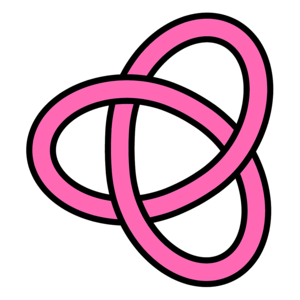
\includegraphics[width=\linewidth]{../data/knots/3_1.png}
        \subcaption{$3_{1}$}
    \end{minipage}
    \begin{minipage}[b]{.18\linewidth}
        \centering
        
\includegraphics[width=\linewidth]{../data/knots/4_1.png}
        \subcaption{$4_{1}$}
    \end{minipage}
    \begin{minipage}[b]{.18\linewidth}
        \centering
        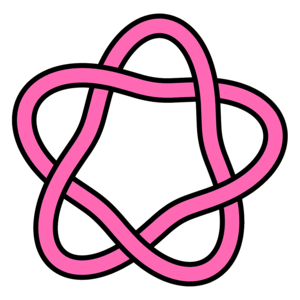
\includegraphics[width=\linewidth]{../data/knots/5_1.png}
        \subcaption{$5_{1}$}
    \end{minipage}
    \begin{minipage}[b]{.18\linewidth}
        \centering
        
\includegraphics[width=\linewidth]{../data/knots/5_2.png}
        \subcaption{$5_{2}$}
    \end{minipage}
    \begin{minipage}[b]{.18\linewidth}
        \centering
        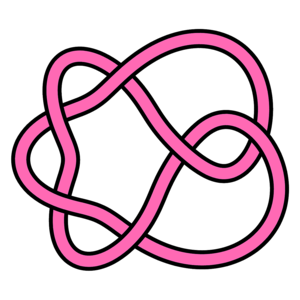
\includegraphics[width=\linewidth]{../data/knots/6_1.png}
        \subcaption{$6_{1}$}
    \end{minipage}
\end{figure}
\begin{figure}[H]
    \begin{minipage}[b]{.18\linewidth}
        \centering
        
\includegraphics[width=\linewidth]{../data/knots/6_2.png}
        \subcaption{$6_{2}$}
    \end{minipage}
    \begin{minipage}[b]{.18\linewidth}
        \centering
        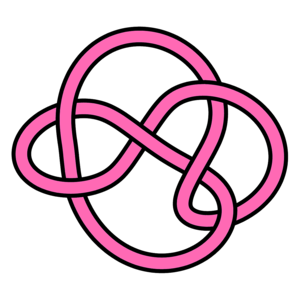
\includegraphics[width=\linewidth]{../data/knots/6_3.png}
        \subcaption{$6_{3}$}
    \end{minipage}
    \begin{minipage}[b]{.18\linewidth}
        \centering
        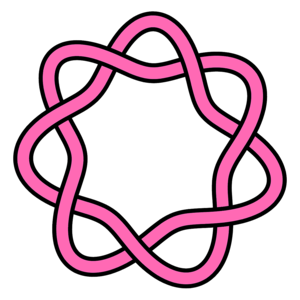
\includegraphics[width=\linewidth]{../data/knots/7_1.png}
        \subcaption{$7_{1}$}
    \end{minipage}
    \begin{minipage}[b]{.18\linewidth}
        \centering
        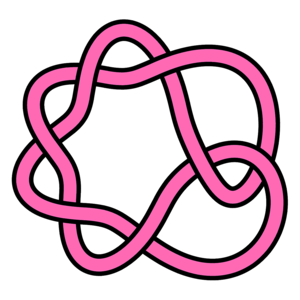
\includegraphics[width=\linewidth]{../data/knots/7_2.png}
        \subcaption{$7_{2}$}
    \end{minipage}
    \begin{minipage}[b]{.18\linewidth}
        \centering
        
\includegraphics[width=\linewidth]{../data/knots/7_3.png}
        \subcaption{$7_{3}$}
    \end{minipage}
\end{figure}
\begin{figure}[H]
    \begin{minipage}[b]{.18\linewidth}
        \centering
        
\includegraphics[width=\linewidth]{../data/knots/7_4.png}
        \subcaption{$7_{4}$}
    \end{minipage}
    \begin{minipage}[b]{.18\linewidth}
        \centering
        
\includegraphics[width=\linewidth]{../data/knots/7_5.png}
        \subcaption{$7_{5}$}
    \end{minipage}
    \begin{minipage}[b]{.18\linewidth}
        \centering
        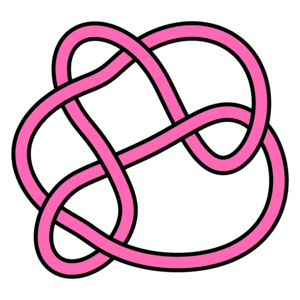
\includegraphics[width=\linewidth]{../data/knots/7_6.png}
        \subcaption{$7_{6}$}
    \end{minipage}
    \begin{minipage}[b]{.18\linewidth}
        \centering
        
\includegraphics[width=\linewidth]{../data/knots/7_7.png}
        \subcaption{$7_{7}$}
    \end{minipage}
    \begin{minipage}[b]{.18\linewidth}
        \centering
        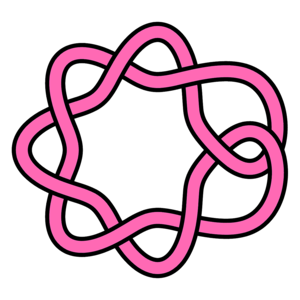
\includegraphics[width=\linewidth]{../data/knots/8_1.png}
        \subcaption{$8_{1}$}
    \end{minipage}
\end{figure}
\begin{figure}[H]
    \begin{minipage}[b]{.18\linewidth}
        \centering
        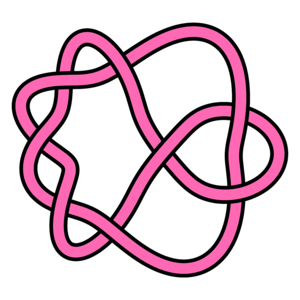
\includegraphics[width=\linewidth]{../data/knots/8_2.png}
        \subcaption{$8_{2}$}
    \end{minipage}
    \begin{minipage}[b]{.18\linewidth}
        \centering
        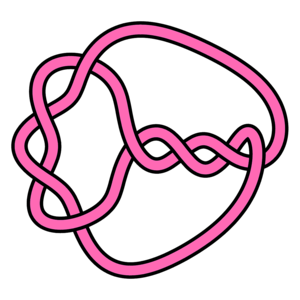
\includegraphics[width=\linewidth]{../data/knots/8_3.png}
        \subcaption{$8_{3}$}
    \end{minipage}
    \begin{minipage}[b]{.18\linewidth}
        \centering
        
\includegraphics[width=\linewidth]{../data/knots/8_4.png}
        \subcaption{$8_{4}$}
    \end{minipage}
    \begin{minipage}[b]{.18\linewidth}
        \centering
        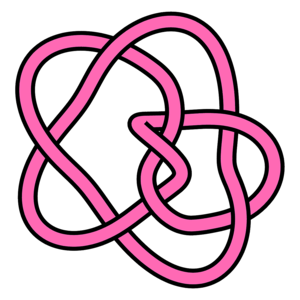
\includegraphics[width=\linewidth]{../data/knots/8_5.png}
        \subcaption{$8_{5}$}
    \end{minipage}
    \begin{minipage}[b]{.18\linewidth}
        \centering
        
\includegraphics[width=\linewidth]{../data/knots/8_6.png}
        \subcaption{$8_{6}$}
    \end{minipage}
\end{figure}
\begin{figure}[H]
    \begin{minipage}[b]{.18\linewidth}
        \centering
        
\includegraphics[width=\linewidth]{../data/knots/8_7.png}
        \subcaption{$8_{7}$}
    \end{minipage}
    \begin{minipage}[b]{.18\linewidth}
        \centering
        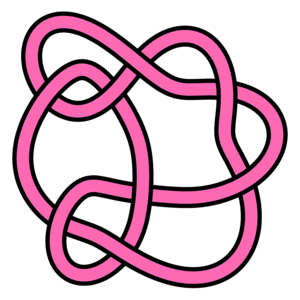
\includegraphics[width=\linewidth]{../data/knots/8_8.png}
        \subcaption{$8_{8}$}
    \end{minipage}
    \begin{minipage}[b]{.18\linewidth}
        \centering
        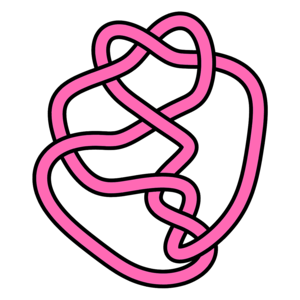
\includegraphics[width=\linewidth]{../data/knots/8_9.png}
        \subcaption{$8_{9}$}
    \end{minipage}
    \begin{minipage}[b]{.18\linewidth}
        \centering
        
\includegraphics[width=\linewidth]{../data/knots/8_10.png}
        \subcaption{$8_{10}$}
    \end{minipage}
    \begin{minipage}[b]{.18\linewidth}
        \centering
        
\includegraphics[width=\linewidth]{../data/knots/8_11.png}
        \subcaption{$8_{11}$}
    \end{minipage}
\end{figure}
\begin{figure}[H]
    \begin{minipage}[b]{.18\linewidth}
        \centering
        
\includegraphics[width=\linewidth]{../data/knots/8_12.png}
        \subcaption{$8_{12}$}
    \end{minipage}
    \begin{minipage}[b]{.18\linewidth}
        \centering
        
\includegraphics[width=\linewidth]{../data/knots/8_13.png}
        \subcaption{$8_{13}$}
    \end{minipage}
    \begin{minipage}[b]{.18\linewidth}
        \centering
        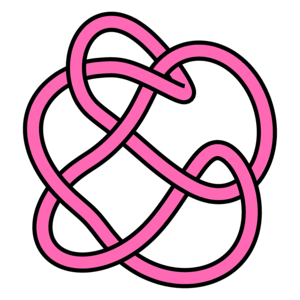
\includegraphics[width=\linewidth]{../data/knots/8_14.png}
        \subcaption{$8_{14}$}
    \end{minipage}
    \begin{minipage}[b]{.18\linewidth}
        \centering
        
\includegraphics[width=\linewidth]{../data/knots/8_15.png}
        \subcaption{$8_{15}$}
    \end{minipage}
    \begin{minipage}[b]{.18\linewidth}
        \centering
        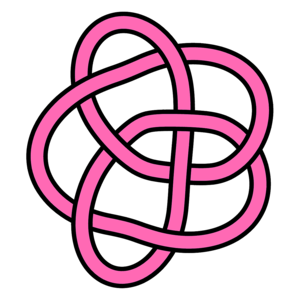
\includegraphics[width=\linewidth]{../data/knots/8_16.png}
        \subcaption{$8_{16}$}
    \end{minipage}
\end{figure}
\begin{figure}[H]
    \begin{minipage}[b]{.18\linewidth}
        \centering
        \includegraphics[width=\linewidth]{../data/knots/8_17.png}
        \subcaption{$8_{17}$}
    \end{minipage}
    \begin{minipage}[b]{.18\linewidth}
        \centering
        \includegraphics[width=\linewidth]{../data/knots/8_18.png}
        \subcaption{$8_{18}$}
    \end{minipage}
    \begin{minipage}[b]{.18\linewidth}
        \centering
        \includegraphics[width=\linewidth]{../data/knots/8_19.png}
        \subcaption{$8_{19}$}
    \end{minipage}
    \begin{minipage}[b]{.18\linewidth}
        \centering
        \includegraphics[width=\linewidth]{../data/knots/8_20.png}
        \subcaption{$8_{20}$}
    \end{minipage}
    \begin{minipage}[b]{.18\linewidth}
        \centering
        \includegraphics[width=\linewidth]{../data/knots/8_21.png}
        \subcaption{$8_{21}$}
    \end{minipage}
\end{figure}
\begin{figure}[H]
    \begin{minipage}[b]{.18\linewidth}
        \centering
        \includegraphics[width=\linewidth]{../data/knots/9_1.png}
        \subcaption{$9_{1}$}
    \end{minipage}
    \begin{minipage}[b]{.18\linewidth}
        \centering
        \includegraphics[width=\linewidth]{../data/knots/9_2.png}
        \subcaption{$9_{2}$}
    \end{minipage}
    \begin{minipage}[b]{.18\linewidth}
        \centering
        \includegraphics[width=\linewidth]{../data/knots/9_3.png}
        \subcaption{$9_{3}$}
    \end{minipage}
    \begin{minipage}[b]{.18\linewidth}
        \centering
        \includegraphics[width=\linewidth]{../data/knots/9_4.png}
        \subcaption{$9_{4}$}
    \end{minipage}
    \begin{minipage}[b]{.18\linewidth}
        \centering
        \includegraphics[width=\linewidth]{../data/knots/9_5.png}
        \subcaption{$9_{5}$}
    \end{minipage}
\end{figure}
\begin{figure}[H]
    \begin{minipage}[b]{.18\linewidth}
        \centering
        \includegraphics[width=\linewidth]{../data/knots/9_6.png}
        \subcaption{$9_{6}$}
    \end{minipage}
    \begin{minipage}[b]{.18\linewidth}
        \centering
        \includegraphics[width=\linewidth]{../data/knots/9_7.png}
        \subcaption{$9_{7}$}
    \end{minipage}
    \begin{minipage}[b]{.18\linewidth}
        \centering
        \includegraphics[width=\linewidth]{../data/knots/9_8.png}
        \subcaption{$9_{8}$}
    \end{minipage}
    \begin{minipage}[b]{.18\linewidth}
        \centering
        \includegraphics[width=\linewidth]{../data/knots/9_9.png}
        \subcaption{$9_{9}$}
    \end{minipage}
    \begin{minipage}[b]{.18\linewidth}
        \centering
        \includegraphics[width=\linewidth]{../data/knots/9_10.png}
        \subcaption{$9_{10}$}
    \end{minipage}
\end{figure}
\begin{figure}[H]
    \begin{minipage}[b]{.18\linewidth}
        \centering
        \includegraphics[width=\linewidth]{../data/knots/9_11.png}
        \subcaption{$9_{11}$}
    \end{minipage}
    \begin{minipage}[b]{.18\linewidth}
        \centering
        \includegraphics[width=\linewidth]{../data/knots/9_12.png}
        \subcaption{$9_{12}$}
    \end{minipage}
    \begin{minipage}[b]{.18\linewidth}
        \centering
        \includegraphics[width=\linewidth]{../data/knots/9_13.png}
        \subcaption{$9_{13}$}
    \end{minipage}
    \begin{minipage}[b]{.18\linewidth}
        \centering
        \includegraphics[width=\linewidth]{../data/knots/9_14.png}
        \subcaption{$9_{14}$}
    \end{minipage}
    \begin{minipage}[b]{.18\linewidth}
        \centering
        \includegraphics[width=\linewidth]{../data/knots/9_15.png}
        \subcaption{$9_{15}$}
    \end{minipage}
\end{figure}
\begin{figure}[H]
    \begin{minipage}[b]{.18\linewidth}
        \centering
        \includegraphics[width=\linewidth]{../data/knots/9_16.png}
        \subcaption{$9_{16}$}
    \end{minipage}
    \begin{minipage}[b]{.18\linewidth}
        \centering
        \includegraphics[width=\linewidth]{../data/knots/9_17.png}
        \subcaption{$9_{17}$}
    \end{minipage}
    \begin{minipage}[b]{.18\linewidth}
        \centering
        \includegraphics[width=\linewidth]{../data/knots/9_18.png}
        \subcaption{$9_{18}$}
    \end{minipage}
    \begin{minipage}[b]{.18\linewidth}
        \centering
        \includegraphics[width=\linewidth]{../data/knots/9_19.png}
        \subcaption{$9_{19}$}
    \end{minipage}
    \begin{minipage}[b]{.18\linewidth}
        \centering
        \includegraphics[width=\linewidth]{../data/knots/9_20.png}
        \subcaption{$9_{20}$}
    \end{minipage}
\end{figure}
\begin{figure}[H]
    \begin{minipage}[b]{.18\linewidth}
        \centering
        \includegraphics[width=\linewidth]{../data/knots/9_21.png}
        \subcaption{$9_{21}$}
    \end{minipage}
    \begin{minipage}[b]{.18\linewidth}
        \centering
        \includegraphics[width=\linewidth]{../data/knots/9_22.png}
        \subcaption{$9_{22}$}
    \end{minipage}
    \begin{minipage}[b]{.18\linewidth}
        \centering
        \includegraphics[width=\linewidth]{../data/knots/9_23.png}
        \subcaption{$9_{23}$}
    \end{minipage}
    \begin{minipage}[b]{.18\linewidth}
        \centering
        \includegraphics[width=\linewidth]{../data/knots/9_24.png}
        \subcaption{$9_{24}$}
    \end{minipage}
    \begin{minipage}[b]{.18\linewidth}
        \centering
        \includegraphics[width=\linewidth]{../data/knots/9_25.png}
        \subcaption{$9_{25}$}
    \end{minipage}
\end{figure}
\begin{figure}[H]
    \begin{minipage}[b]{.18\linewidth}
        \centering
        \includegraphics[width=\linewidth]{../data/knots/9_26.png}
        \subcaption{$9_{26}$}
    \end{minipage}
    \begin{minipage}[b]{.18\linewidth}
        \centering
        \includegraphics[width=\linewidth]{../data/knots/9_27.png}
        \subcaption{$9_{27}$}
    \end{minipage}
    \begin{minipage}[b]{.18\linewidth}
        \centering
        \includegraphics[width=\linewidth]{../data/knots/9_28.png}
        \subcaption{$9_{28}$}
    \end{minipage}
    \begin{minipage}[b]{.18\linewidth}
        \centering
        \includegraphics[width=\linewidth]{../data/knots/9_29.png}
        \subcaption{$9_{29}$}
    \end{minipage}
    \begin{minipage}[b]{.18\linewidth}
        \centering
        \includegraphics[width=\linewidth]{../data/knots/9_30.png}
        \subcaption{$9_{30}$}
    \end{minipage}
\end{figure}
\begin{figure}[H]
    \begin{minipage}[b]{.18\linewidth}
        \centering
        \includegraphics[width=\linewidth]{../data/knots/9_31.png}
        \subcaption{$9_{31}$}
    \end{minipage}
    \begin{minipage}[b]{.18\linewidth}
        \centering
        \includegraphics[width=\linewidth]{../data/knots/9_32.png}
        \subcaption{$9_{32}$}
    \end{minipage}
    \begin{minipage}[b]{.18\linewidth}
        \centering
        \includegraphics[width=\linewidth]{../data/knots/9_33.png}
        \subcaption{$9_{33}$}
    \end{minipage}
    \begin{minipage}[b]{.18\linewidth}
        \centering
        \includegraphics[width=\linewidth]{../data/knots/9_34.png}
        \subcaption{$9_{34}$}
    \end{minipage}
    \begin{minipage}[b]{.18\linewidth}
        \centering
        \includegraphics[width=\linewidth]{../data/knots/9_35.png}
        \subcaption{$9_{35}$}
    \end{minipage}
\end{figure}
\begin{figure}[H]
    \begin{minipage}[b]{.18\linewidth}
        \centering
        \includegraphics[width=\linewidth]{../data/knots/9_36.png}
        \subcaption{$9_{36}$}
    \end{minipage}
    \begin{minipage}[b]{.18\linewidth}
        \centering
        \includegraphics[width=\linewidth]{../data/knots/9_37.png}
        \subcaption{$9_{37}$}
    \end{minipage}
    \begin{minipage}[b]{.18\linewidth}
        \centering
        \includegraphics[width=\linewidth]{../data/knots/9_38.png}
        \subcaption{$9_{38}$}
    \end{minipage}
    \begin{minipage}[b]{.18\linewidth}
        \centering
        \includegraphics[width=\linewidth]{../data/knots/9_39.png}
        \subcaption{$9_{39}$}
    \end{minipage}
    \begin{minipage}[b]{.18\linewidth}
        \centering
        \includegraphics[width=\linewidth]{../data/knots/9_40.png}
        \subcaption{$9_{40}$}
    \end{minipage}
\end{figure}
\begin{figure}[H]
    \begin{minipage}[b]{.18\linewidth}
        \centering
        \includegraphics[width=\linewidth]{../data/knots/9_41.png}
        \subcaption{$9_{41}$}
    \end{minipage}
    \begin{minipage}[b]{.18\linewidth}
        \centering
        \includegraphics[width=\linewidth]{../data/knots/9_42.png}
        \subcaption{$9_{42}$}
    \end{minipage}
    \begin{minipage}[b]{.18\linewidth}
        \centering
        \includegraphics[width=\linewidth]{../data/knots/9_43.png}
        \subcaption{$9_{43}$}
    \end{minipage}
    \begin{minipage}[b]{.18\linewidth}
        \centering
        \includegraphics[width=\linewidth]{../data/knots/9_44.png}
        \subcaption{$9_{44}$}
    \end{minipage}
    \begin{minipage}[b]{.18\linewidth}
        \centering
        \includegraphics[width=\linewidth]{../data/knots/9_45.png}
        \subcaption{$9_{45}$}
    \end{minipage}
\end{figure}
\begin{figure}[H]
    \begin{minipage}[b]{.18\linewidth}
        \centering
        \includegraphics[width=\linewidth]{../data/knots/9_46.png}
        \subcaption{$9_{46}$}
    \end{minipage}
    \begin{minipage}[b]{.18\linewidth}
        \centering
        \includegraphics[width=\linewidth]{../data/knots/9_47.png}
        \subcaption{$9_{47}$}
    \end{minipage}
    \begin{minipage}[b]{.18\linewidth}
        \centering
        \includegraphics[width=\linewidth]{../data/knots/9_48.png}
        \subcaption{$9_{48}$}
    \end{minipage}
    \begin{minipage}[b]{.18\linewidth}
        \centering
        \includegraphics[width=\linewidth]{../data/knots/9_49.png}
        \subcaption{$9_{49}$}
    \end{minipage}
    \begin{minipage}[b]{.18\linewidth}
        \centering
        \includegraphics[width=\linewidth]{../data/knots/10_1.png}
        \subcaption{$10_{1}$}
    \end{minipage}
\end{figure}
\begin{figure}[H]
    \begin{minipage}[b]{.18\linewidth}
        \centering
        \includegraphics[width=\linewidth]{../data/knots/10_2.png}
        \subcaption{$10_{2}$}
    \end{minipage}
    \begin{minipage}[b]{.18\linewidth}
        \centering
        \includegraphics[width=\linewidth]{../data/knots/10_3.png}
        \subcaption{$10_{3}$}
    \end{minipage}
    \begin{minipage}[b]{.18\linewidth}
        \centering
        \includegraphics[width=\linewidth]{../data/knots/10_4.png}
        \subcaption{$10_{4}$}
    \end{minipage}
    \begin{minipage}[b]{.18\linewidth}
        \centering
        \includegraphics[width=\linewidth]{../data/knots/10_5.png}
        \subcaption{$10_{5}$}
    \end{minipage}
    \begin{minipage}[b]{.18\linewidth}
        \centering
        \includegraphics[width=\linewidth]{../data/knots/10_6.png}
        \subcaption{$10_{6}$}
    \end{minipage}
\end{figure}
\begin{figure}[H]
    \begin{minipage}[b]{.18\linewidth}
        \centering
        \includegraphics[width=\linewidth]{../data/knots/10_7.png}
        \subcaption{$10_{7}$}
    \end{minipage}
    \begin{minipage}[b]{.18\linewidth}
        \centering
        \includegraphics[width=\linewidth]{../data/knots/10_8.png}
        \subcaption{$10_{8}$}
    \end{minipage}
    \begin{minipage}[b]{.18\linewidth}
        \centering
        \includegraphics[width=\linewidth]{../data/knots/10_9.png}
        \subcaption{$10_{9}$}
    \end{minipage}
    \begin{minipage}[b]{.18\linewidth}
        \centering
        \includegraphics[width=\linewidth]{../data/knots/10_10.png}
        \subcaption{$10_{10}$}
    \end{minipage}
    \begin{minipage}[b]{.18\linewidth}
        \centering
        \includegraphics[width=\linewidth]{../data/knots/10_11.png}
        \subcaption{$10_{11}$}
    \end{minipage}
\end{figure}
\begin{figure}[H]
    \begin{minipage}[b]{.18\linewidth}
        \centering
        \includegraphics[width=\linewidth]{../data/knots/10_12.png}
        \subcaption{$10_{12}$}
    \end{minipage}
    \begin{minipage}[b]{.18\linewidth}
        \centering
        \includegraphics[width=\linewidth]{../data/knots/10_13.png}
        \subcaption{$10_{13}$}
    \end{minipage}
    \begin{minipage}[b]{.18\linewidth}
        \centering
        \includegraphics[width=\linewidth]{../data/knots/10_14.png}
        \subcaption{$10_{14}$}
    \end{minipage}
    \begin{minipage}[b]{.18\linewidth}
        \centering
        \includegraphics[width=\linewidth]{../data/knots/10_15.png}
        \subcaption{$10_{15}$}
    \end{minipage}
    \begin{minipage}[b]{.18\linewidth}
        \centering
        \includegraphics[width=\linewidth]{../data/knots/10_16.png}
        \subcaption{$10_{16}$}
    \end{minipage}
\end{figure}
\begin{figure}[H]
    \begin{minipage}[b]{.18\linewidth}
        \centering
        \includegraphics[width=\linewidth]{../data/knots/10_17.png}
        \subcaption{$10_{17}$}
    \end{minipage}
    \begin{minipage}[b]{.18\linewidth}
        \centering
        \includegraphics[width=\linewidth]{../data/knots/10_18.png}
        \subcaption{$10_{18}$}
    \end{minipage}
    \begin{minipage}[b]{.18\linewidth}
        \centering
        \includegraphics[width=\linewidth]{../data/knots/10_19.png}
        \subcaption{$10_{19}$}
    \end{minipage}
    \begin{minipage}[b]{.18\linewidth}
        \centering
        \includegraphics[width=\linewidth]{../data/knots/10_20.png}
        \subcaption{$10_{20}$}
    \end{minipage}
    \begin{minipage}[b]{.18\linewidth}
        \centering
        \includegraphics[width=\linewidth]{../data/knots/10_21.png}
        \subcaption{$10_{21}$}
    \end{minipage}
\end{figure}
\begin{figure}[H]
    \begin{minipage}[b]{.18\linewidth}
        \centering
        \includegraphics[width=\linewidth]{../data/knots/10_22.png}
        \subcaption{$10_{22}$}
    \end{minipage}
    \begin{minipage}[b]{.18\linewidth}
        \centering
        \includegraphics[width=\linewidth]{../data/knots/10_23.png}
        \subcaption{$10_{23}$}
    \end{minipage}
    \begin{minipage}[b]{.18\linewidth}
        \centering
        \includegraphics[width=\linewidth]{../data/knots/10_24.png}
        \subcaption{$10_{24}$}
    \end{minipage}
    \begin{minipage}[b]{.18\linewidth}
        \centering
        \includegraphics[width=\linewidth]{../data/knots/10_25.png}
        \subcaption{$10_{25}$}
    \end{minipage}
    \begin{minipage}[b]{.18\linewidth}
        \centering
        \includegraphics[width=\linewidth]{../data/knots/10_26.png}
        \subcaption{$10_{26}$}
    \end{minipage}
\end{figure}
\begin{figure}[H]
    \begin{minipage}[b]{.18\linewidth}
        \centering
        \includegraphics[width=\linewidth]{../data/knots/10_27.png}
        \subcaption{$10_{27}$}
    \end{minipage}
    \begin{minipage}[b]{.18\linewidth}
        \centering
        \includegraphics[width=\linewidth]{../data/knots/10_28.png}
        \subcaption{$10_{28}$}
    \end{minipage}
    \begin{minipage}[b]{.18\linewidth}
        \centering
        \includegraphics[width=\linewidth]{../data/knots/10_29.png}
        \subcaption{$10_{29}$}
    \end{minipage}
    \begin{minipage}[b]{.18\linewidth}
        \centering
        \includegraphics[width=\linewidth]{../data/knots/10_30.png}
        \subcaption{$10_{30}$}
    \end{minipage}
    \begin{minipage}[b]{.18\linewidth}
        \centering
        \includegraphics[width=\linewidth]{../data/knots/10_31.png}
        \subcaption{$10_{31}$}
    \end{minipage}
\end{figure}
\begin{figure}[H]
    \begin{minipage}[b]{.18\linewidth}
        \centering
        \includegraphics[width=\linewidth]{../data/knots/10_32.png}
        \subcaption{$10_{32}$}
    \end{minipage}
    \begin{minipage}[b]{.18\linewidth}
        \centering
        \includegraphics[width=\linewidth]{../data/knots/10_33.png}
        \subcaption{$10_{33}$}
    \end{minipage}
    \begin{minipage}[b]{.18\linewidth}
        \centering
        \includegraphics[width=\linewidth]{../data/knots/10_34.png}
        \subcaption{$10_{34}$}
    \end{minipage}
    \begin{minipage}[b]{.18\linewidth}
        \centering
        \includegraphics[width=\linewidth]{../data/knots/10_35.png}
        \subcaption{$10_{35}$}
    \end{minipage}
    \begin{minipage}[b]{.18\linewidth}
        \centering
        \includegraphics[width=\linewidth]{../data/knots/10_36.png}
        \subcaption{$10_{36}$}
    \end{minipage}
\end{figure}
\begin{figure}[H]
    \begin{minipage}[b]{.18\linewidth}
        \centering
        \includegraphics[width=\linewidth]{../data/knots/10_37.png}
        \subcaption{$10_{37}$}
    \end{minipage}
    \begin{minipage}[b]{.18\linewidth}
        \centering
        \includegraphics[width=\linewidth]{../data/knots/10_38.png}
        \subcaption{$10_{38}$}
    \end{minipage}
    \begin{minipage}[b]{.18\linewidth}
        \centering
        \includegraphics[width=\linewidth]{../data/knots/10_39.png}
        \subcaption{$10_{39}$}
    \end{minipage}
    \begin{minipage}[b]{.18\linewidth}
        \centering
        \includegraphics[width=\linewidth]{../data/knots/10_40.png}
        \subcaption{$10_{40}$}
    \end{minipage}
    \begin{minipage}[b]{.18\linewidth}
        \centering
        \includegraphics[width=\linewidth]{../data/knots/10_41.png}
        \subcaption{$10_{41}$}
    \end{minipage}
\end{figure}
\begin{figure}[H]
    \begin{minipage}[b]{.18\linewidth}
        \centering
        \includegraphics[width=\linewidth]{../data/knots/10_42.png}
        \subcaption{$10_{42}$}
    \end{minipage}
    \begin{minipage}[b]{.18\linewidth}
        \centering
        \includegraphics[width=\linewidth]{../data/knots/10_43.png}
        \subcaption{$10_{43}$}
    \end{minipage}
    \begin{minipage}[b]{.18\linewidth}
        \centering
        \includegraphics[width=\linewidth]{../data/knots/10_44.png}
        \subcaption{$10_{44}$}
    \end{minipage}
    \begin{minipage}[b]{.18\linewidth}
        \centering
        \includegraphics[width=\linewidth]{../data/knots/10_45.png}
        \subcaption{$10_{45}$}
    \end{minipage}
    \begin{minipage}[b]{.18\linewidth}
        \centering
        \includegraphics[width=\linewidth]{../data/knots/10_46.png}
        \subcaption{$10_{46}$}
    \end{minipage}
\end{figure}
\begin{figure}[H]
    \begin{minipage}[b]{.18\linewidth}
        \centering
        \includegraphics[width=\linewidth]{../data/knots/10_47.png}
        \subcaption{$10_{47}$}
    \end{minipage}
    \begin{minipage}[b]{.18\linewidth}
        \centering
        \includegraphics[width=\linewidth]{../data/knots/10_48.png}
        \subcaption{$10_{48}$}
    \end{minipage}
    \begin{minipage}[b]{.18\linewidth}
        \centering
        \includegraphics[width=\linewidth]{../data/knots/10_49.png}
        \subcaption{$10_{49}$}
    \end{minipage}
    \begin{minipage}[b]{.18\linewidth}
        \centering
        \includegraphics[width=\linewidth]{../data/knots/10_50.png}
        \subcaption{$10_{50}$}
    \end{minipage}
    \begin{minipage}[b]{.18\linewidth}
        \centering
        \includegraphics[width=\linewidth]{../data/knots/10_51.png}
        \subcaption{$10_{51}$}
    \end{minipage}
\end{figure}
\begin{figure}[H]
    \begin{minipage}[b]{.18\linewidth}
        \centering
        \includegraphics[width=\linewidth]{../data/knots/10_52.png}
        \subcaption{$10_{52}$}
    \end{minipage}
    \begin{minipage}[b]{.18\linewidth}
        \centering
        \includegraphics[width=\linewidth]{../data/knots/10_53.png}
        \subcaption{$10_{53}$}
    \end{minipage}
    \begin{minipage}[b]{.18\linewidth}
        \centering
        \includegraphics[width=\linewidth]{../data/knots/10_54.png}
        \subcaption{$10_{54}$}
    \end{minipage}
    \begin{minipage}[b]{.18\linewidth}
        \centering
        \includegraphics[width=\linewidth]{../data/knots/10_55.png}
        \subcaption{$10_{55}$}
    \end{minipage}
    \begin{minipage}[b]{.18\linewidth}
        \centering
        \includegraphics[width=\linewidth]{../data/knots/10_56.png}
        \subcaption{$10_{56}$}
    \end{minipage}
\end{figure}
\begin{figure}[H]
    \begin{minipage}[b]{.18\linewidth}
        \centering
        \includegraphics[width=\linewidth]{../data/knots/10_57.png}
        \subcaption{$10_{57}$}
    \end{minipage}
    \begin{minipage}[b]{.18\linewidth}
        \centering
        \includegraphics[width=\linewidth]{../data/knots/10_58.png}
        \subcaption{$10_{58}$}
    \end{minipage}
    \begin{minipage}[b]{.18\linewidth}
        \centering
        \includegraphics[width=\linewidth]{../data/knots/10_59.png}
        \subcaption{$10_{59}$}
    \end{minipage}
    \begin{minipage}[b]{.18\linewidth}
        \centering
        \includegraphics[width=\linewidth]{../data/knots/10_60.png}
        \subcaption{$10_{60}$}
    \end{minipage}
    \begin{minipage}[b]{.18\linewidth}
        \centering
        \includegraphics[width=\linewidth]{../data/knots/10_61.png}
        \subcaption{$10_{61}$}
    \end{minipage}
\end{figure}
\begin{figure}[H]
    \begin{minipage}[b]{.18\linewidth}
        \centering
        \includegraphics[width=\linewidth]{../data/knots/10_62.png}
        \subcaption{$10_{62}$}
    \end{minipage}
    \begin{minipage}[b]{.18\linewidth}
        \centering
        \includegraphics[width=\linewidth]{../data/knots/10_63.png}
        \subcaption{$10_{63}$}
    \end{minipage}
    \begin{minipage}[b]{.18\linewidth}
        \centering
        \includegraphics[width=\linewidth]{../data/knots/10_64.png}
        \subcaption{$10_{64}$}
    \end{minipage}
    \begin{minipage}[b]{.18\linewidth}
        \centering
        \includegraphics[width=\linewidth]{../data/knots/10_65.png}
        \subcaption{$10_{65}$}
    \end{minipage}
    \begin{minipage}[b]{.18\linewidth}
        \centering
        \includegraphics[width=\linewidth]{../data/knots/10_66.png}
        \subcaption{$10_{66}$}
    \end{minipage}
\end{figure}
\begin{figure}[H]
    \begin{minipage}[b]{.18\linewidth}
        \centering
        \includegraphics[width=\linewidth]{../data/knots/10_67.png}
        \subcaption{$10_{67}$}
    \end{minipage}
    \begin{minipage}[b]{.18\linewidth}
        \centering
        \includegraphics[width=\linewidth]{../data/knots/10_68.png}
        \subcaption{$10_{68}$}
    \end{minipage}
    \begin{minipage}[b]{.18\linewidth}
        \centering
        \includegraphics[width=\linewidth]{../data/knots/10_69.png}
        \subcaption{$10_{69}$}
    \end{minipage}
    \begin{minipage}[b]{.18\linewidth}
        \centering
        \includegraphics[width=\linewidth]{../data/knots/10_70.png}
        \subcaption{$10_{70}$}
    \end{minipage}
    \begin{minipage}[b]{.18\linewidth}
        \centering
        \includegraphics[width=\linewidth]{../data/knots/10_71.png}
        \subcaption{$10_{71}$}
    \end{minipage}
\end{figure}
\begin{figure}[H]
    \begin{minipage}[b]{.18\linewidth}
        \centering
        \includegraphics[width=\linewidth]{../data/knots/10_72.png}
        \subcaption{$10_{72}$}
    \end{minipage}
    \begin{minipage}[b]{.18\linewidth}
        \centering
        \includegraphics[width=\linewidth]{../data/knots/10_73.png}
        \subcaption{$10_{73}$}
    \end{minipage}
    \begin{minipage}[b]{.18\linewidth}
        \centering
        \includegraphics[width=\linewidth]{../data/knots/10_74.png}
        \subcaption{$10_{74}$}
    \end{minipage}
    \begin{minipage}[b]{.18\linewidth}
        \centering
        \includegraphics[width=\linewidth]{../data/knots/10_75.png}
        \subcaption{$10_{75}$}
    \end{minipage}
    \begin{minipage}[b]{.18\linewidth}
        \centering
        \includegraphics[width=\linewidth]{../data/knots/10_76.png}
        \subcaption{$10_{76}$}
    \end{minipage}
\end{figure}
\begin{figure}[H]
    \begin{minipage}[b]{.18\linewidth}
        \centering
        \includegraphics[width=\linewidth]{../data/knots/10_77.png}
        \subcaption{$10_{77}$}
    \end{minipage}
    \begin{minipage}[b]{.18\linewidth}
        \centering
        \includegraphics[width=\linewidth]{../data/knots/10_78.png}
        \subcaption{$10_{78}$}
    \end{minipage}
    \begin{minipage}[b]{.18\linewidth}
        \centering
        \includegraphics[width=\linewidth]{../data/knots/10_79.png}
        \subcaption{$10_{79}$}
    \end{minipage}
    \begin{minipage}[b]{.18\linewidth}
        \centering
        \includegraphics[width=\linewidth]{../data/knots/10_80.png}
        \subcaption{$10_{80}$}
    \end{minipage}
    \begin{minipage}[b]{.18\linewidth}
        \centering
        \includegraphics[width=\linewidth]{../data/knots/10_81.png}
        \subcaption{$10_{81}$}
    \end{minipage}
\end{figure}
\begin{figure}[H]
    \begin{minipage}[b]{.18\linewidth}
        \centering
        \includegraphics[width=\linewidth]{../data/knots/10_82.png}
        \subcaption{$10_{82}$}
    \end{minipage}
    \begin{minipage}[b]{.18\linewidth}
        \centering
        \includegraphics[width=\linewidth]{../data/knots/10_83.png}
        \subcaption{$10_{83}$}
    \end{minipage}
    \begin{minipage}[b]{.18\linewidth}
        \centering
        \includegraphics[width=\linewidth]{../data/knots/10_84.png}
        \subcaption{$10_{84}$}
    \end{minipage}
    \begin{minipage}[b]{.18\linewidth}
        \centering
        \includegraphics[width=\linewidth]{../data/knots/10_85.png}
        \subcaption{$10_{85}$}
    \end{minipage}
    \begin{minipage}[b]{.18\linewidth}
        \centering
        \includegraphics[width=\linewidth]{../data/knots/10_86.png}
        \subcaption{$10_{86}$}
    \end{minipage}
\end{figure}
\begin{figure}[H]
    \begin{minipage}[b]{.18\linewidth}
        \centering
        \includegraphics[width=\linewidth]{../data/knots/10_87.png}
        \subcaption{$10_{87}$}
    \end{minipage}
    \begin{minipage}[b]{.18\linewidth}
        \centering
        \includegraphics[width=\linewidth]{../data/knots/10_88.png}
        \subcaption{$10_{88}$}
    \end{minipage}
    \begin{minipage}[b]{.18\linewidth}
        \centering
        \includegraphics[width=\linewidth]{../data/knots/10_89.png}
        \subcaption{$10_{89}$}
    \end{minipage}
    \begin{minipage}[b]{.18\linewidth}
        \centering
        \includegraphics[width=\linewidth]{../data/knots/10_90.png}
        \subcaption{$10_{90}$}
    \end{minipage}
    \begin{minipage}[b]{.18\linewidth}
        \centering
        \includegraphics[width=\linewidth]{../data/knots/10_91.png}
        \subcaption{$10_{91}$}
    \end{minipage}
\end{figure}
\begin{figure}[H]
    \begin{minipage}[b]{.18\linewidth}
        \centering
        \includegraphics[width=\linewidth]{../data/knots/10_92.png}
        \subcaption{$10_{92}$}
    \end{minipage}
    \begin{minipage}[b]{.18\linewidth}
        \centering
        \includegraphics[width=\linewidth]{../data/knots/10_93.png}
        \subcaption{$10_{93}$}
    \end{minipage}
    \begin{minipage}[b]{.18\linewidth}
        \centering
        \includegraphics[width=\linewidth]{../data/knots/10_94.png}
        \subcaption{$10_{94}$}
    \end{minipage}
    \begin{minipage}[b]{.18\linewidth}
        \centering
        \includegraphics[width=\linewidth]{../data/knots/10_95.png}
        \subcaption{$10_{95}$}
    \end{minipage}
    \begin{minipage}[b]{.18\linewidth}
        \centering
        \includegraphics[width=\linewidth]{../data/knots/10_96.png}
        \subcaption{$10_{96}$}
    \end{minipage}
\end{figure}
\begin{figure}[H]
    \begin{minipage}[b]{.18\linewidth}
        \centering
        \includegraphics[width=\linewidth]{../data/knots/10_97.png}
        \subcaption{$10_{97}$}
    \end{minipage}
    \begin{minipage}[b]{.18\linewidth}
        \centering
        \includegraphics[width=\linewidth]{../data/knots/10_98.png}
        \subcaption{$10_{98}$}
    \end{minipage}
    \begin{minipage}[b]{.18\linewidth}
        \centering
        \includegraphics[width=\linewidth]{../data/knots/10_99.png}
        \subcaption{$10_{99}$}
    \end{minipage}
    \begin{minipage}[b]{.18\linewidth}
        \centering
        \includegraphics[width=\linewidth]{../data/knots/10_100.png}
        \subcaption{$10_{100}$}
    \end{minipage}
    \begin{minipage}[b]{.18\linewidth}
        \centering
        \includegraphics[width=\linewidth]{../data/knots/10_101.png}
        \subcaption{$10_{101}$}
    \end{minipage}
\end{figure}
\begin{figure}[H]
    \begin{minipage}[b]{.18\linewidth}
        \centering
        \includegraphics[width=\linewidth]{../data/knots/10_102.png}
        \subcaption{$10_{102}$}
    \end{minipage}
    \begin{minipage}[b]{.18\linewidth}
        \centering
        \includegraphics[width=\linewidth]{../data/knots/10_103.png}
        \subcaption{$10_{103}$}
    \end{minipage}
    \begin{minipage}[b]{.18\linewidth}
        \centering
        \includegraphics[width=\linewidth]{../data/knots/10_104.png}
        \subcaption{$10_{104}$}
    \end{minipage}
    \begin{minipage}[b]{.18\linewidth}
        \centering
        \includegraphics[width=\linewidth]{../data/knots/10_105.png}
        \subcaption{$10_{105}$}
    \end{minipage}
    \begin{minipage}[b]{.18\linewidth}
        \centering
        \includegraphics[width=\linewidth]{../data/knots/10_106.png}
        \subcaption{$10_{106}$}
    \end{minipage}
\end{figure}
\begin{figure}[H]
    \begin{minipage}[b]{.18\linewidth}
        \centering
        \includegraphics[width=\linewidth]{../data/knots/10_107.png}
        \subcaption{$10_{107}$}
    \end{minipage}
    \begin{minipage}[b]{.18\linewidth}
        \centering
        \includegraphics[width=\linewidth]{../data/knots/10_108.png}
        \subcaption{$10_{108}$}
    \end{minipage}
    \begin{minipage}[b]{.18\linewidth}
        \centering
        \includegraphics[width=\linewidth]{../data/knots/10_109.png}
        \subcaption{$10_{109}$}
    \end{minipage}
    \begin{minipage}[b]{.18\linewidth}
        \centering
        \includegraphics[width=\linewidth]{../data/knots/10_110.png}
        \subcaption{$10_{110}$}
    \end{minipage}
    \begin{minipage}[b]{.18\linewidth}
        \centering
        \includegraphics[width=\linewidth]{../data/knots/10_111.png}
        \subcaption{$10_{111}$}
    \end{minipage}
\end{figure}
\begin{figure}[H]
    \begin{minipage}[b]{.18\linewidth}
        \centering
        \includegraphics[width=\linewidth]{../data/knots/10_112.png}
        \subcaption{$10_{112}$}
    \end{minipage}
    \begin{minipage}[b]{.18\linewidth}
        \centering
        \includegraphics[width=\linewidth]{../data/knots/10_113.png}
        \subcaption{$10_{113}$}
    \end{minipage}
    \begin{minipage}[b]{.18\linewidth}
        \centering
        \includegraphics[width=\linewidth]{../data/knots/10_114.png}
        \subcaption{$10_{114}$}
    \end{minipage}
    \begin{minipage}[b]{.18\linewidth}
        \centering
        \includegraphics[width=\linewidth]{../data/knots/10_115.png}
        \subcaption{$10_{115}$}
    \end{minipage}
    \begin{minipage}[b]{.18\linewidth}
        \centering
        \includegraphics[width=\linewidth]{../data/knots/10_116.png}
        \subcaption{$10_{116}$}
    \end{minipage}
\end{figure}
\begin{figure}[H]
    \begin{minipage}[b]{.18\linewidth}
        \centering
        \includegraphics[width=\linewidth]{../data/knots/10_117.png}
        \subcaption{$10_{117}$}
    \end{minipage}
    \begin{minipage}[b]{.18\linewidth}
        \centering
        \includegraphics[width=\linewidth]{../data/knots/10_118.png}
        \subcaption{$10_{118}$}
    \end{minipage}
    \begin{minipage}[b]{.18\linewidth}
        \centering
        \includegraphics[width=\linewidth]{../data/knots/10_119.png}
        \subcaption{$10_{119}$}
    \end{minipage}
    \begin{minipage}[b]{.18\linewidth}
        \centering
        \includegraphics[width=\linewidth]{../data/knots/10_120.png}
        \subcaption{$10_{120}$}
    \end{minipage}
    \begin{minipage}[b]{.18\linewidth}
        \centering
        \includegraphics[width=\linewidth]{../data/knots/10_121.png}
        \subcaption{$10_{121}$}
    \end{minipage}
\end{figure}
\begin{figure}[H]
    \begin{minipage}[b]{.18\linewidth}
        \centering
        \includegraphics[width=\linewidth]{../data/knots/10_122.png}
        \subcaption{$10_{122}$}
    \end{minipage}
    \begin{minipage}[b]{.18\linewidth}
        \centering
        \includegraphics[width=\linewidth]{../data/knots/10_123.png}
        \subcaption{$10_{123}$}
    \end{minipage}
    \begin{minipage}[b]{.18\linewidth}
        \centering
        \includegraphics[width=\linewidth]{../data/knots/10_124.png}
        \subcaption{$10_{124}$}
    \end{minipage}
    \begin{minipage}[b]{.18\linewidth}
        \centering
        \includegraphics[width=\linewidth]{../data/knots/10_125.png}
        \subcaption{$10_{125}$}
    \end{minipage}
    \begin{minipage}[b]{.18\linewidth}
        \centering
        \includegraphics[width=\linewidth]{../data/knots/10_126.png}
        \subcaption{$10_{126}$}
    \end{minipage}
\end{figure}
\begin{figure}[H]
    \begin{minipage}[b]{.18\linewidth}
        \centering
        \includegraphics[width=\linewidth]{../data/knots/10_127.png}
        \subcaption{$10_{127}$}
    \end{minipage}
    \begin{minipage}[b]{.18\linewidth}
        \centering
        \includegraphics[width=\linewidth]{../data/knots/10_128.png}
        \subcaption{$10_{128}$}
    \end{minipage}
    \begin{minipage}[b]{.18\linewidth}
        \centering
        \includegraphics[width=\linewidth]{../data/knots/10_129.png}
        \subcaption{$10_{129}$}
    \end{minipage}
    \begin{minipage}[b]{.18\linewidth}
        \centering
        \includegraphics[width=\linewidth]{../data/knots/10_130.png}
        \subcaption{$10_{130}$}
    \end{minipage}
    \begin{minipage}[b]{.18\linewidth}
        \centering
        \includegraphics[width=\linewidth]{../data/knots/10_131.png}
        \subcaption{$10_{131}$}
    \end{minipage}
\end{figure}
\begin{figure}[H]
    \begin{minipage}[b]{.18\linewidth}
        \centering
        \includegraphics[width=\linewidth]{../data/knots/10_132.png}
        \subcaption{$10_{132}$}
    \end{minipage}
    \begin{minipage}[b]{.18\linewidth}
        \centering
        \includegraphics[width=\linewidth]{../data/knots/10_133.png}
        \subcaption{$10_{133}$}
    \end{minipage}
    \begin{minipage}[b]{.18\linewidth}
        \centering
        \includegraphics[width=\linewidth]{../data/knots/10_134.png}
        \subcaption{$10_{134}$}
    \end{minipage}
    \begin{minipage}[b]{.18\linewidth}
        \centering
        \includegraphics[width=\linewidth]{../data/knots/10_135.png}
        \subcaption{$10_{135}$}
    \end{minipage}
    \begin{minipage}[b]{.18\linewidth}
        \centering
        \includegraphics[width=\linewidth]{../data/knots/10_136.png}
        \subcaption{$10_{136}$}
    \end{minipage}
\end{figure}
\begin{figure}[H]
    \begin{minipage}[b]{.18\linewidth}
        \centering
        \includegraphics[width=\linewidth]{../data/knots/10_137.png}
        \subcaption{$10_{137}$}
    \end{minipage}
    \begin{minipage}[b]{.18\linewidth}
        \centering
        \includegraphics[width=\linewidth]{../data/knots/10_138.png}
        \subcaption{$10_{138}$}
    \end{minipage}
    \begin{minipage}[b]{.18\linewidth}
        \centering
        \includegraphics[width=\linewidth]{../data/knots/10_139.png}
        \subcaption{$10_{139}$}
    \end{minipage}
    \begin{minipage}[b]{.18\linewidth}
        \centering
        \includegraphics[width=\linewidth]{../data/knots/10_140.png}
        \subcaption{$10_{140}$}
    \end{minipage}
    \begin{minipage}[b]{.18\linewidth}
        \centering
        \includegraphics[width=\linewidth]{../data/knots/10_141.png}
        \subcaption{$10_{141}$}
    \end{minipage}
\end{figure}
\begin{figure}[H]
    \begin{minipage}[b]{.18\linewidth}
        \centering
        \includegraphics[width=\linewidth]{../data/knots/10_142.png}
        \subcaption{$10_{142}$}
    \end{minipage}
    \begin{minipage}[b]{.18\linewidth}
        \centering
        \includegraphics[width=\linewidth]{../data/knots/10_143.png}
        \subcaption{$10_{143}$}
    \end{minipage}
    \begin{minipage}[b]{.18\linewidth}
        \centering
        \includegraphics[width=\linewidth]{../data/knots/10_144.png}
        \subcaption{$10_{144}$}
    \end{minipage}
    \begin{minipage}[b]{.18\linewidth}
        \centering
        \includegraphics[width=\linewidth]{../data/knots/10_145.png}
        \subcaption{$10_{145}$}
    \end{minipage}
    \begin{minipage}[b]{.18\linewidth}
        \centering
        \includegraphics[width=\linewidth]{../data/knots/10_146.png}
        \subcaption{$10_{146}$}
    \end{minipage}
\end{figure}
\begin{figure}[H]
    \begin{minipage}[b]{.18\linewidth}
        \centering
        \includegraphics[width=\linewidth]{../data/knots/10_147.png}
        \subcaption{$10_{147}$}
    \end{minipage}
    \begin{minipage}[b]{.18\linewidth}
        \centering
        \includegraphics[width=\linewidth]{../data/knots/10_148.png}
        \subcaption{$10_{148}$}
    \end{minipage}
    \begin{minipage}[b]{.18\linewidth}
        \centering
        \includegraphics[width=\linewidth]{../data/knots/10_149.png}
        \subcaption{$10_{149}$}
    \end{minipage}
    \begin{minipage}[b]{.18\linewidth}
        \centering
        \includegraphics[width=\linewidth]{../data/knots/10_150.png}
        \subcaption{$10_{150}$}
    \end{minipage}
    \begin{minipage}[b]{.18\linewidth}
        \centering
        \includegraphics[width=\linewidth]{../data/knots/10_151.png}
        \subcaption{$10_{151}$}
    \end{minipage}
\end{figure}
\begin{figure}[H]
    \begin{minipage}[b]{.18\linewidth}
        \centering
        \includegraphics[width=\linewidth]{../data/knots/10_152.png}
        \subcaption{$10_{152}$}
    \end{minipage}
    \begin{minipage}[b]{.18\linewidth}
        \centering
        \includegraphics[width=\linewidth]{../data/knots/10_153.png}
        \subcaption{$10_{153}$}
    \end{minipage}
    \begin{minipage}[b]{.18\linewidth}
        \centering
        \includegraphics[width=\linewidth]{../data/knots/10_154.png}
        \subcaption{$10_{154}$}
    \end{minipage}
    \begin{minipage}[b]{.18\linewidth}
        \centering
        \includegraphics[width=\linewidth]{../data/knots/10_155.png}
        \subcaption{$10_{155}$}
    \end{minipage}
    \begin{minipage}[b]{.18\linewidth}
        \centering
        \includegraphics[width=\linewidth]{../data/knots/10_156.png}
        \subcaption{$10_{156}$}
    \end{minipage}
\end{figure}
\begin{figure}[H]
    \begin{minipage}[b]{.18\linewidth}
        \centering
        \includegraphics[width=\linewidth]{../data/knots/10_157.png}
        \subcaption{$10_{157}$}
    \end{minipage}
    \begin{minipage}[b]{.18\linewidth}
        \centering
        \includegraphics[width=\linewidth]{../data/knots/10_158.png}
        \subcaption{$10_{158}$}
    \end{minipage}
    \begin{minipage}[b]{.18\linewidth}
        \centering
        \includegraphics[width=\linewidth]{../data/knots/10_159.png}
        \subcaption{$10_{159}$}
    \end{minipage}
    \begin{minipage}[b]{.18\linewidth}
        \centering
        \includegraphics[width=\linewidth]{../data/knots/10_160.png}
        \subcaption{$10_{160}$}
    \end{minipage}
    \begin{minipage}[b]{.18\linewidth}
        \centering
        \includegraphics[width=\linewidth]{../data/knots/10_161.png}
        \subcaption{$10_{161}$}
    \end{minipage}
\end{figure}
\begin{figure}[H]
    \begin{minipage}[b]{.18\linewidth}
        \centering
        \includegraphics[width=\linewidth]{../data/knots/10_162.png}
        \subcaption{$10_{162}$}
    \end{minipage}
    \begin{minipage}[b]{.18\linewidth}
        \centering
        \includegraphics[width=\linewidth]{../data/knots/10_163.png}
        \subcaption{$10_{163}$}
    \end{minipage}
    \begin{minipage}[b]{.18\linewidth}
        \centering
        \includegraphics[width=\linewidth]{../data/knots/10_164.png}
        \subcaption{$10_{164}$}
    \end{minipage}
    \begin{minipage}[b]{.18\linewidth}
        \centering
        \includegraphics[width=\linewidth]{../data/knots/10_165.png}
        \subcaption{$10_{165}$}
    \end{minipage}
\end{figure}
\end{comment}



\raggedright
\bibliographystyle{plain}
%\bibliographystyle{plunsrt}
\bibliography{knot_theory}

\newpage
\listoftodos[Lista rzeczy do poprawienia]
\end{document}